% exemplo genérico de uso da classe iiufrgs.cls
% $Id: iiufrgs.tex,v 1.1.1.1 2005/01/18 23:54:42 avila Exp $
%
% This is an example file and is hereby explicitly put in the
% public domain.
%
%\documentclass[pgmicro,mestrado,english]{iiufrgs}

\documentclass[pgmicro,diss,english]{iiufrgs}
\usepackage[alf,abnt-emphasize=bf]{abntex2cite}
% um tipo específico de monografia pode ser informado como parâmetro opcional:
%\documentclass[tese]{iiufrgs}
% monografias em inglês devem receber o parâmetro `english':
%\documentclass[diss,english]{iiufrgs}0
% a opção `openright' pode ser usada para forçar inícios de capítulos
% em páginas ímpares
% \documentclass[openright]{iiufrgs}
% para gerar uma versão somente-frente, basta utilizar a opção `oneside':
% \documentclass[oneside]{iiufrgs}
\usepackage[T1]{fontenc}        % pacote para conj. de caracteres correto
\usepackage[utf8]{inputenc}   % pacote para acentuação
\usepackage{graphicx}           % pacote para importar figuras
\usepackage{times}              % pacote para usar fonte Adobe Times
\usepackage{textcomp}
\usepackage{mathptmx}          % p/ usar fonte Adobe Times nas fórmulas
\usepackage{caption}
\usepackage{subcaption}
\usepackage{multirow}
\usepackage[normalem]{ulem}
\usepackage{pdfpages}
\usepackage{listings}
\usepackage{amsmath}
\usepackage{array}
\usepackage{bibentry}
%\usepackage{natbib}

%\nobibliography*

\newenvironment{conditions}
	{\par\vspace{\abovedisplayskip}\noindent\begin{tabular}{>{$}l<{$} @{${}={}$} l}}
	{\end{tabular}\par\vspace{\belowdisplayskip}}
%\usepackage{biblatex}
%\usepackage{filecontents}
%\usepackage{natbib}
%\usepackage{bibentry}
%
% Informações gerais
%
%\addbibresource{biblio.bib}
\title{Schmitt Trigger Dimensioning Under Variability and Voltage Scaling for Minimum Energy Operation}

\author{de Moraes}{Leonardo Barlette}
% alguns documentos podem ter varios autores:
%\author{Flaumann}{Frida Gutenberg}
%\author{Flaumann}{Klaus Gutenberg}

% orientador e co-orientador são opcionais (não diga isso pra eles :))
\advisor[Prof.~Dr.]{Reis}{Ricardo}
\coadvisor[Profa.~Dra.]{Meinhardt}{Cristina}

% a data deve ser a da defesa; se nao especificada, são gerados
% mes e ano correntes
%\date{maio}{2001}

% o nome do curso pode ser redefinido (ex. para TCs)
%\course{Curso de Especialização em Cachaça}

% o local de realização do trabalho pode ser especificado (ex. para TCs)
% com o comando \location:
%\location{Itaquaquecetuba}{SP}

% itens individuais da nominata podem ser redefinidos com os comandos
% abaixo:
% \renewcommand{\nominataReit}{Prof\textsuperscript{a}.~Wrana Maria Panizzi}
% \renewcommand{\nominataReitname}{Reitora}
% \renewcommand{\nominataPRE}{Prof.~Jos{\'e} Carlos Ferraz Hennemann}
% \renewcommand{\nominataPREname}{Pr{\'o}-Reitor de Ensino}
% \renewcommand{\nominataPRAPG}{Prof\textsuperscript{a}.~Joc{\'e}lia Grazia}
% \renewcommand{\nominataPRAPGname}{Pr{\'o}-Reitora Adjunta de P{\'o}s-Gradua{\c{c}}{\~a}o}
% \renewcommand{\nominataDir}{Prof.~Philippe Olivier Alexandre Navaux}
% \renewcommand{\nominataDirname}{Diretor do Instituto de Inform{\'a}tica}
% \renewcommand{\nominataCoord}{Prof.~Carlos Alberto Heuser}
% \renewcommand{\nominataCoordname}{Coordenador do PPGC}
% \renewcommand{\nominataBibchefe}{Beatriz Regina Bastos Haro}
% \renewcommand{\nominataBibchefename}{Bibliotec{\'a}ria-chefe do Instituto de Inform{\'a}tica}
% \renewcommand{\nominataChefeINA}{Prof.~Jos{\'e} Valdeni de Lima}
% \renewcommand{\nominataChefeINAname}{Chefe do \deptINA}
% \renewcommand{\nominataChefeINT}{Prof.~Leila Ribeiro}
% \renewcommand{\nominataChefeINTname}{Chefe do \deptINT}

% A seguir são apresentados comandos específicos para alguns
% tipos de documentos.

% Relatório de Pesquisa [rp]:
% \rp{123}             % numero do rp
% \financ{CNPq, CAPES} % orgaos financiadores

% Trabalho Individual [ti]:
% \ti{1}     % numero do TI
% \ti[II]{456} % no caso de ser o segundo TI

% Trabalho de Conclusão [tc]:
% além de definir explicitamente o nome do curso (\course) e o local
% de realização (\location), é necessário redefinir a nominata,
% pois as informações necessárias dependem do curso. Ex.:
\renewcommand{\nominata}{
        UNIVERSIDADE FEDERAL DO RIO GRANDE DO SUL\\
        Reitor: Prof.~Rui Vicente Oppermann\\
        Vice-Reitora: Prof.\textsuperscript{a}~Jane Fraga Tutikian\\
	Pró-Reitor de Pós-Graduação: Prof.~Celso Giannetti Loureiro Chaves\\
        Diretora do Instituto de Informática: Prof.\textsuperscript{a}~Carla Maria Dal Sasso Freitas\\
        Coordenador do PGMICRO: Prof.~Tiago Roberto Balen\\
        Bibliotecária-chefe do Instituto de Informática: Beatriz Regina Bastos Haro
}

% Monografias de Especialização [espec]:
% \espec{Redes e Sistemas Distribuídos}      % nome do curso
% \coord[Profa.~Dra.]{Weber}{Taisy da Silva} % coordenador do curso
% \dept{INA}                                 % departamento relacionado

%
% palavras-chave
% iniciar todas com letras minúsculas, exceto no caso de abreviaturas
%
\keyword{Process Variability}
\keyword{FinFET}
\keyword{Energy}
\keyword{Schmitt Trigger}
\keyword{Full Adder}
\keyword{Microelectronics}
%\addbibresource{biblio.bib}

%
% inicio do documento
%
\begin{document}

% folha de rosto
% às vezes é necessário redefinir algum comando logo antes de produzir
% a folha de rosto:
% \renewcommand{\coordname}{Coordenadora do Curso}
\maketitle

% dedicatoria
% \clearpage
% \begin{flushright}
% \mbox{}\vfill
% {\sffamily\itshape
% ``If I have seen farther than others,\\
% it is because I stood on the shoulders of giants.''\\}
% --- \textsc{Sir~Isaac Newton}
% \end{flushright}

% agradecimentos
% \chapter*{Agradecimentos}
% Agradeço ao \LaTeX\ por não ter vírus de macro\ldots

\newpage
% sumario


% lista de abreviaturas e siglas
% o parametro deve ser a abreviatura mais longa
\begin{listofabbrv}{SPMD}
        \item[IoT] Internet of Things
        \item[CMOS] Complementary Metal Oxide Semiconductor
        \item[ULP] Ultra Low Power
        \item[FinFET] Fin Field Effect Transistor
        \item[SCE] Short Channel Effect
        \item[RDF] Random Dopant Fluctuation
        \item[ST] Schmitt Trigger
        \item[FA] Full Adder
        \item[$V_T$] Threshold Voltage
        \item[NBTI] Negative Bias Temperature Instability
        \item[HCI] Hot Carrier Injection
        \item[CMP] Chemical-Mechanical Polishing
        \item[LER] Line-Edge Roughness
        \item[WF] Work Function
        \item[FET] Field Effect Transistor
        \item[MOSFET] Metal Oxide Semiconductor Field Effect Transistor
        \item[PVT] Process Voltage and Temperature
        \item[WID] Within-Die
        \item[SIMD] Single Instruction Multiple Data
        \item[PDP] Power Delay Product
        \item[TGA] Transmission Gate Adder
        \item[TFA] Transmission Function Adder
        \item[CPL] Complementary Pass Transistor Logic
        \item[CNFET] Carbon Nanotube Field Effect Transistor
        \item[FDSOI] Fully Depleted Silicon On Insulator
        \item[OTS] Optimal Transistor Sizing
        \item[$L$] Gate Length
        \item[$W_{FIN}$] Fin Width
        \item[$H_{FIN}$] Fin Height
        \item[$T_{OX}$] Oxide Thickness
        \item[SOI] Silicon On Insulator
        \item[WFF] Work Function Fluctuation
        \item[SRAM] Static Random Access Memory
        \item[GOBD] Gate Oxide Break Down
        \item[ECC] Error Correcting Code
        \item[SNM] Static Noise Margin
        \item[UDSM] Ultra-Deep Sub-Micron
        \item[VTC] Voltage Transfer Curve
        \item[DRC] Design Rule Checking
        \item[LVS] Layout Versus Schematic
        \item[EDA] Electronic Design Automation
        \item[PDK] Process Design Kit
        \item[ASAP] Arizona State Predictive PDK
        \item[FEOL] Front End Of Line
        \item[MOL] Middle End Of Line
        \item[BEOL] Back End Of Line
        \item[SDT] Source-Drain Trench
        \item[LIG] Local-Interconnect Gate
        \item[LISD] Local-Interconnect Source-Drain
        \item[V0] Via 0
        \item[M1] Metal 1
        \item[M2] Metal 2
        \item[MC] Monte Carlo
        \item[EDP] Energy Deviation Product
        \item[TIST] Triple-Inverter ST
        \item[SIG] Stacked-Inverter Gate
\end{listofabbrv}

% idem para a lista de símbolos
%\begin{listofsymbols}{$\alpha\beta\pi\omega$}
%       \item[$\sum{\frac{a}{b}}$] Somatório do produtório
%       \item[$\alpha\beta\pi\omega$] Fator de inconstância do resultado
%\end{listofsymbols}

% lista de figuras
\listoffigures

% lista de tabelas
%\listoftables

% resumo na língua do documento
\begin{abstract}
{Technology scaling alongside the increasing process variability impact in modern technology nodes are the main reasons to control deviations over metrics in IC nanometer designs. Also, given the increasing set of devices working in battery-oriented environments, energy consumption should be minimal and the operation regime reliable. Schmitt Triggers are traditionally used for noise immunity enhancement, and have been recently applied to mitigate radiation effects and process variability impact. However, Schmitt Trigger operation at the nominal voltage introduces higher power consumption, in comparison to an inverter, making the application of Schmitt Trigger in ultra low power applications difficult. Thus, this work main contribution is to trace the relationship between transistor sizing, supply voltage, and process variability to get a low energy consumption circuit while still keeping low levels of deviations due to the impact of process-induced variability. The results are extracted from three different designs of inverters. All simulations are performed upon the extracted layouts design at 7-nm with the FinFET technology. Each layout presents a different number of fins, where each simulation presents a different level of variability and supply voltage. Amongst the several metrics considered - propagation times, energy, hysteresis interval, current ratios, voltage gains, and slopes - the energy is the prioritized metrics with an analysis considering different kinds of applications - low energy, low sensibility, and cost-benefit - being performed. Given so, it is shown that a cost-benefit analysis can highlight sets of sizing and supply voltage where it can provide a 37.51\% decrease on energy consumption while only increasing its sensibility by 7.42\%. Furthermore, it is presented that the dependence of supply voltage and sensibility to process variability is not directly related, with slight decreases in the supply voltages bringing better results. Considering the average measures, the inverter is still the fastest and most energy-efficient circuit, presenting the highest performance, lowest energy consumption, and smallest area. Although, when comparing noise immunity characteristics, the 6-Transistor Schmitt Trigger presents the highest noise margins and slopes, with higher current ratios, and gains. The TIST designs present the highest current ratios, gains, and hysteresis ratios. The improvements, although, do not come without respective increases in propagations times, energy consumption, and area.}
\end{abstract}

% ^ qual circuito tem melhores vantagens e em quais métricas?

% resumo na outra língua
% como parametros devem ser passados o titulo e as palavras-chave
% na outra língua, separadas por vírgulas
\begin{englishabstract}
{
Dimensionamento de inversores sob influência de variabilidade de processo e diminuição da  tensão de alimentação para operação com consumo mínimo.
}{Variabilidade de Processo, FinFET, Energia, \textit{Schmitt Trigger}, Somadores Completos, Microeletrônica}
{

A miniaturização da tecnologia de trasistores, juntamente com o crescente impacto da variabilidade de processo nos nodos tecnológicos modernos são a principal razão para o esforço da indústria em investir nos métodos para controle dos efeitos de variabilidade nas métricas dos circuitos integrados. Além disso, dado o crescimento exponencial do número de aplicações dependendes de bateria, o consumo de energia deve-se manter mínimo e o regime de operação estável. Circuitos \textit{Schmitt Trigger} são tradicionalmente aplicados para melhora da resistência de circuitos integrados ao ruído e foram recentemente aplicados para mitigar os efeitos da radiação e do impacto da variabilidade. Contudo, a operação de \textit{Schmitt Triggers} em tensão nominal introduz alto consumo de potência, tornando a adoção de \textit{Schmitt Triggers} em cenários de ultra baixa potência, díficil. Assim, a principal contribuição deste trabalho é traçar a relação entre dimensionamento dos transistores, tensão de alimentação e variabilidade de processo, para alcançar o menor possível consumo de energia, mas mantendo a robustez aos efeitos de variabilidade em níveis aceitáveis. Os resultados são extraídos de três tipos de inversores, entre eles \textit{Schmitt Triggers}. Todas as simulações são realizadas considerando os leiautes extraídos projetados em 7nm com a tecnologia de transistores FinFET. Cada leiaute apresenta um numero diferente de \textit{fins}, onde cada simulação apresenta um nível diferente de variabilidade de processo e tensão de alimentação. Entre diversas métricas consideradas - tempos de propagação, energia, intervalo de histerese, razões entre as correntes dinâmica e estática, ganhos de tensão e inclinação dos sinais - as medidas de energia são priorizadas, com uma análise considerando diferentes tipos de aplicações - baixa energia, máxima robustez e custo-benefício. A partir dos resultados, é demonstrado que uma análise de custo-benefício pode destacar conjuntos de dimensionamentos e tensões de alimentação que podem prover uma redução de até 37.51\% no consumo de energia com um aumento de somente 7.42\% na sensibilidade aos efeitos de variabilidade. Além disso, é demonstrado que a dependência da tensão de alimentação e a robustez aos efeitos da variabilidade de processo não é direta, com pequenas diminuições na tensão de alimentação resultando em ganhos na robustez. Nas medidas médias das métricas, o inversor tradicional ainda é o circuito mais rápido e mais energéticamente eficiente, apresentando o melhor desempenho,  menor consumo de energia e menor área. Porém, quando comparando características que provêem imuidade ao ruído, o \textit{Schmitt Trigger} de seis transistores apresentou as maiores margens de ruído, com maiores razões das correntes e ganhos. Já o circuito TIST apresentou as maiores razões entre correntes, ganhos e intervalos de histerese. Entretanto, estas melhorias não vem sem as respectivas penalidades nos tempos de propagação, consumo de energia e area.

}
\end{englishabstract}

\tableofcontents

\chapter{Introduction}
%\section{Internet of Things / Ultra Low Power Applications}
	Technology scaling, as stated by Moore where the number of transistors in a chip should double at about every two years, is a major factor in the ascendance of Integrated Circuits (ICs), providing higher transistor densities and voltage scaling due to the miniaturization of gate dimensions, internal capacitances and resistances. Such improvements provided the IC designers with plenty processing power per area unit of a chip and energy efficiency, making it the perfect combination for the usage of ICs in mobile applications \cite{islam:10}.

	As devices shrank, several transistor characteristic became severe problems for the modern semiconductor industry, alongside some new challenges. As transistors got smaller, the supply voltage decreased as well, to accomodate appropriate currents to an evermore smaller channel. Although, as the supply voltage decreases the noise margins got narrower, with the smaller currents, and capacitances curbing the circuit ability to mask the transients caused by external noise and radiation \cite{abbas:15}.

	Furthermore, variations into the device's geometrical and electrical parameters were always a reality, introducing minor, if not negligible, variations into the circuits behavior. Even though, those geometrical variations did not scale down at the same rate as the devices. It has gotten increasingly difficult to produce further smaller light waves to correctly print such small patterns. Additionally, modern devices are so close to the atomic limit, that even variations in the scale of few units to few hundreds of atoms can exert influence into the device behavior, decreasing yield \cite{abbas:15}.

    One of the many categories of systems which emerged from the techonology scaling is The Internet of Things (IoT) which turned out to be one of the major mainstream trends, shaping technology development and the industry. The IoT concept englobes the shift from an internet which is used to interconnect end-user devices to, nowadays, interconnect physical objects that communicate with each other and/or with humans \cite{miorandi2012internet}. The IoT rise, alongside battery technology improvements, has provided us with portable, powerful and useful equipment for our daily routine, with wireless communication making information available anytime and anywhere \cite{manoli2010energy}.

    IoT devices have been applied in many different scenarios, from improving building maintenance, to sensoring remote areas for environmental observation and even in cars, for better safety and comfort. However, while many devices have to be connected to the power grid, sensor nodes are expected to be self-sufficient. Additionally, batteries, the traditional means of powering self-sufficient systems, need to be replaced and/or charged, which means maintenance must be frequently performed \cite{bleitner2018comparison}. Given that, energy harvesting in combination with rechargeable batteries has become a viable way to alleviate the power source and consumption dilemma \cite{manoli2010energy}.

    Energy harvesting makes use of readily available power sources in the vicinity as for example motion or vibration induced kinetic energy, solar and electromagnetic or temperature gradients. A number of viable solutions are already present on the market, like self powered wireless light switches and electro-magnetic generators, which converts vibrations available in industrial plants for powering wireless monitoring sensors \cite{manoli2010energy} \cite{bleitner2018comparison}. Although, regardless of the sensors power supply, it will be always restricted by its power budget, with devices which are able to perform their functionality under heavy power constraints being essential for IoT. In traditional Complementary Metal Oxide Semiconductor (CMOS) circuit design aimed at Ultra Low Power (ULP) applications, the ideal circuit is the one that performs a given task or functionality while consuming the least amount of energy. Such circuits are achieved under transistor sizing and supply voltage tuning, and are technology and application-dependent.

    Nevertheless, the performance of a system operating in its minimum energy per operation point may exceed the power budget of a given application. For example, with an application such as presented in \cite{fojtik2013millimeter}, where the device is only active once per hour, about 80\% of its power consumption is due to standby power. In such a case, the minimization of energy-per-operation seems to be suboptimal in comparison to an idle power minimization kind-of solution. The minimization of supply voltage brings advantage for certain energy harvesting approaches such as thermo-electric. Such harvesting technique can result in DC voltage levels from tens to even hundreds of milivolts \cite{khan2014flexible}.

    One of the industry responses to the challenges related to the improvements in the semiconductor industry is the Fin Field Effect Transistor (FinFET) Technology. FinFET devices present superior channel control due to the reduced Short Channel Effects (SCE) and low (if none) Random Dopant Fluctuation (RDF) effect due to the fully depleted channel \cite{farkhani2014comparative}. Although, at deep technology nodes, variability is, still, one of the most challenging factors, including on FinFET devices. Variability introduces geometrical inconsistencies which changes the circuits behavior in comparison to the final manufactured product. Such changes influence the circuits metrics, hastening its degradation and deviating from its correct operation regime \cite{abbas:15} \cite{nassif:08}.

    Due to the energy constraints of low power applications and the variability impact on recent nodes, the Schmitt Trigger (ST) circuit has been pointed as an alternative. The classical ST has been employed as a key element for several ULP circuits \cite{kulkarni2007160, hays201262, melek:17, lotze2017ultra}. For variability mitigation, mainly attenuating the deviation on the power consumption, and replacing internal inverters on more complex circuits \cite{dokania2015circuit} where spreads in major metrics were successfully limited. Also, the same experiment was executed at electrical and layout levels considering FinFET technology, and showed a considerable decrease in overall variability impact on metrics \cite{toledo2018pros,moraes2018evaluation}. However, with a considerable increase in delay and power consumption.
% In addition to previous work, this work will present further analysis related to this ST technique.

%Furthermore, a considerable part of this work consists of evaluations about the behavior of the classical ST, the Stacked Inverter Gate (SIG) \cite{bose2018stacked} and Triple Inverter Schmitt Trigger (TI-ST) \cite{luo2017sub} over several scenarios of sizing, supply voltage, and process variability level, in order to identify the most apropriate set of characteristics for each design.

	Given all the laid concepts, this work has two main objectives:

	1) to identify an appropriate layout, considering transistor sizing, and supply voltage to achieve the most apropriate design for a set of applications. The considered circuits will be the traditional 6T ST, Stacked Inverter Gate (SIG), Triple Inverter Schmitt Trigger (TIST) and, for the sake of comparison, a traditional inverter. Multiple levels of process variability will be considered. Therefore, depending on manufacturability quality, different recommended layouts and supply voltages can arise.

	2) to apply the ST technique into circuits. In this work, the Full Adder circuit is adopted as a case-study. The technique consists of the replacement of the FAs internal inverters with the respective STs. The considered FAs will be: the Mirror FA, the Transmission Function Adder (TFA), the Transmission Gate Adder (TGA) and Hybrid FA. The two applied STs are the traditional 6T ST and a low-power back-gating-based ST (LPST). The LPST was chosen for demonstrating good results at \cite{dokania2015circuit}. Due to technology restrictions, the LPST design had to be modified, given so, the 6T ST was chosen, in order to provide a reference for comparison and showing desirable results in sub-threshold applications \cite{lotze2017ultra}. All layouts will be designs with a fixed number of transistors and two levels of supply voltages. All simulations will be performed at the same level of process variability.

For both analysis it will be considered the means, standard deviations and normalized standard deviations for the energy and propagation time measures. Specifically for the first analysis, the means, standard deviations and normalized standard deviations will be calculated for further metrics: on and off currents, current ratios and hysteresis interval (when applicable). The output curve slopes and voltage gain will be presented, as well.

    This work is divided into five further sections: Variability Effects on FinFET Technology, where a theoretical foundation about variability is laid with several related works about mitigating its impact in the characteristics of FinFET devices and how process variability presents itself in the device. A section about the considered circuits will explain their functionality and applications. The Methodology Section will explain the experimental setup which will be employed to generate the results. A Results Section is present, showing the extracted measures and related analysis. Lastly, there are a Conclusions and Future Work sections.

\chapter{Process Variability Effects on FinFET Technology}

According to the ITRS Roadmap \cite{blish2003critical}, reliability will become one of the major challenges for the semiconductor industry. The device scaling combined with the adoption of new materials are the source of the increasing yield loss and reliability problems \cite{gielen2008emerging}.

As process technology scaling advanced, decreasing the transistor dimensions, the ratio between device size and atom-size have been decreasing as well. Multiple techniques have been developed to reduce the loss of precision due to the manufacturing process at different end-of-lines. However, as the quantum-mechanical limit approaches, manufacturing-induced imprecision impact rises \cite{asenov1999random} \cite{neuberger2014protecting}.

Variability consists of characteristic deviations, internal or external to the circuit, which can determine its operational features and can be divided in two types concerning its effects, local and global, and three subtypes of variability causes (Environmental, Manufacturing, and Reliability). The general classification can be divided as:

\begin{itemize}

\item Global (Inter-die):

	Global variations are related to the difference in parameter value across identical dies (whether those dies are in the same wafer, on different wafer, in different lots, or even in different fabrication plants).

\item Local (Intra-die):

	Occurs spatially within one chip. It can have a variety of sources, depending on physics of the manufacturing process.

\end{itemize}

	These two types of effects are submitted to 3 subtypes of variability causes:

\begin{itemize}

\item Environmental:

		Mostly external to the circuit, englobes variations in the power supply voltage and temperature. Voltage drops mainly occur due to abrupt changes in the switching activity, inducing large current transients in the system both locally or globally across the die. Local temperature within the die can cause variations in the device mobility and threshold voltages ($V_T$), and wire resistance. It is highly design dependent with timing constants similar to clock frequency \cite{nassif:08} \cite{bernstein2006high}. The intra-die factors include local effects caused by the chip operation such as device voltage variations due to IR drops and ground bounce, delay and slew variations due to crosstalk, input pin capacitance deviations due to slew and state dependency, and differences in temperature inside the chip.

\item Reliability:

	Related to the aging process of the circuit, occurring during its day-to-day operation. Two of the main phenomena are electromigration, due to high enough current densities causing the gradual movement of metal ions due to the electron-ion momentum transfer \cite{young1994failure} \cite{posser2016electromigration} and Hot Carrier Injection (HCI) trapping electrons on oxide which degrades n-MOSFET on-current \cite{takeda1983empirical} \cite{nassif:08} \cite{bernstein2006high}. The intra-die phenomena is mainly represented by the effects of the phenomenon like Negative Bias Temperature Instability (NBTI) which mines the performance of p-channel due to the weakening of Si-H bonds in the oxide generating of interface states and trapping positive charges while the device is operating \cite{wang2008statistical}.

\item Manufacturing:

Defined by device and interconnect geometry variations due to design dependency as well as random material variations. Interconnect width and spacing variations occur mainly due to photolithographic and etch dependencies. Those deviations will impact the interconnect parasitics, resulting in performance and signal degradation. An example is the Chemical-Mechanical Polishing (CMP) relationship between the thickness of the metal and the layout feature density \cite{stine1997analysis}.  Random material variations consist of atomic-level deviations between devices (even when they are identical in layout and geometry) inside the chip. Overall, devices and interconnects will have fully correlated random components, which mean each random component will influence devices and interconnections equally \cite{dietrich2011process}.

Fig. \ref{fig:transAbs}, depicts the transistor intrinsic variability and different levels of abstraction, where from left to right it is shown a typical ideal transistor, a more realistic transitor with variations in its geometrical and electrical parameter, and the atomic-level limit at which we find the transistors in the most modern technologies, where a single atom can make a difference, respectively. These deviations appear in dopant profiles, thickness variations, and Line-Edge Roughness (LER). Dopant fluctuations are the main cause to $V_T$ variations \cite{asenov2003simulation}, with the removal of doping from the channel contributing for the $V_T$ variation reduction, introducing the necessity to set the $V_T$ by gate-metal Work Function (WF) or by biased back gate \cite{frank2001device,wong1999nanoscale}.

Fluctuations in doping levels and device features cause variations in the source/drain regions, which affects the overlap capacitance and the source resistance \cite{frank2000simulation}. LER arises from variations in the total number of incident photons during lithography. Such roughness introduction into the polygons geometry may determine the effective gate width as one moves along the x axis of a Field Effect Transistor (FET) \cite{brunner2003optical}. Another source of random device variability rises from the atomic-scale oxide thickness variation. It can introduce variations in the $V_T$ \cite{asenov2003simulation}, in the oxide tunneling current, and may cause mobility degradation due to the potential variation across the Metal Oxide Semiconductor FET (MOSFET) channel \cite{bernstein2006high}.
The manufacturing factor influencing at intra-die level comprises of geometric and parameter variations in the device and the interconnect derived from the manufacturing process. \textit{Film Thickness} and \textit{Channel Length} variations can result in systematic (not random) differences in $V_T$ and leakage currents between chips in the same wafer. Additionally, deviations in the width in the lower layers of metal due to the congestion and proximity between layers and defects of lithographic nature can impact line resistance as well coupling capacitance. This type of variation is caused by the manufacturing steps: rapid thermal annealing (the wafer is rapidly heated up and cooled down to trigger additional chemical reactions within the photoresist) - with an uneven temperature accross the wafer and by-reticle variability can contribute due to changes in the focus as the mask is stepped across the wafer in the photolithography process - the focus can suffer deviations due to exposure tool lens astigmatisms or by wafer nonplanarity \cite{bernstein2006high, qian2015variability}.

\end{itemize}


    \begin{figure} []
        \centering
        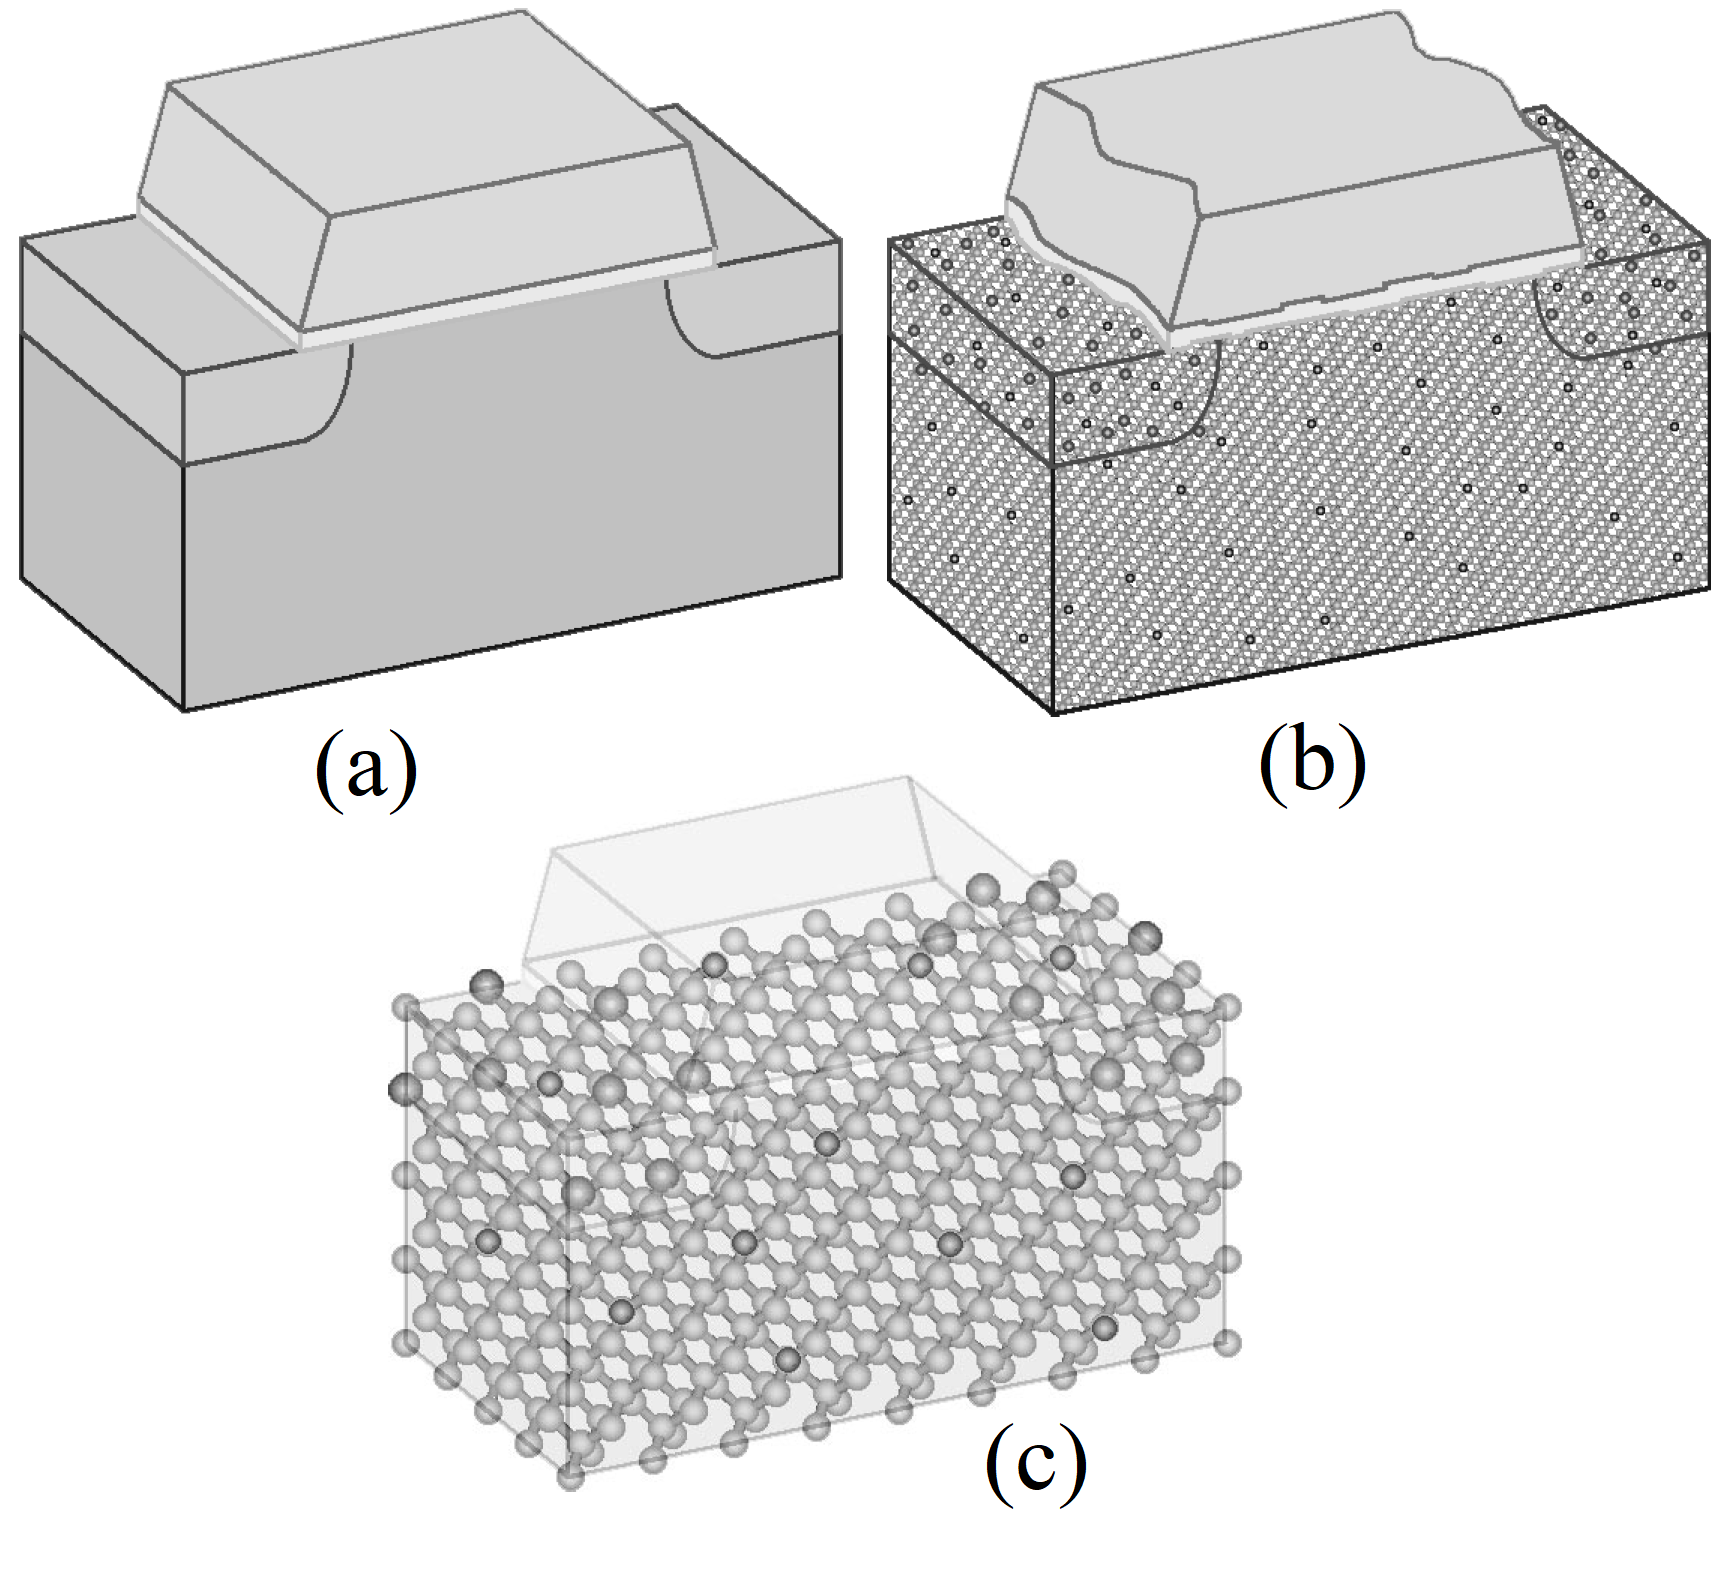
\includegraphics[width=0.8\textwidth, trim={0 0 0 0},clip]{transistorVariability.png}
        \caption{Levels of abstraction from a ideal transistor concept towards a realistic and "atomistic" device concept. (a) Depicts a the current approach of semiconductor device simulation, with continuous dopant charge and smooth boundaries. (b) Depicts a 20-nm MOSFET, with less than 50 Si atoms along the channel. RDF, interface roughness and LER introduce considerable intrinsic parameter fluctuation. (c) Depicts a 4-nm MOSFET, with less than 10 Si atoms along the channel. }
        \label{fig:transAbs}
        \legend{Source: \citet{asenov2003simulation}}
    \end{figure}

% Please add the following required packages to your document preamble:
% \usepackage{graphicx}
\begin{table}[]
\centering
\caption{Impact of variability on performance and power.}
\label{tab:abbastech1}
\resizebox{\textwidth}{!}{%
\begin{tabular}{lcccc}
\hline
\textbf{Property} & \textbf{Ease of measuring} & \textbf{Variability} & \textbf{Effects of variability} & \textbf{Effect of missing specification} \\ \hline
\textbf{Performance} & Medium & Medium: up to 60\% & L, W, R, C, $V_T$, \(\mu\) & Slower product, yield, timing error \\ \hline
\textbf{Leakage Power} & Easy & Large: up to 148\% & L,  $V_T$, \(\mu\), $t_{ox}$ & Shorter battery life, yield, heat \\ \hline
\textbf{Dynamic Power} & Difficult & Workload dependent & C, \(\alpha\) & Shorter battery life, heat \\ \hline
\end{tabular}%
}
\legend{Source: \citet{rahimi2016variability}}
\end{table}

Table \ref{tab:abbastech1} presents the effects of variability and the impact on design, where L and W are the channel length and  width, R and C are the parasitic resistances and capacitances, $V_{T}$ is the threshold voltage, $\mu$ is the semiconductor electron mobility, $t_{ox}$ corresponds to the oxide thickness, and $\alpha$, the ratio between the transistor collector and emitter currents. The impact on power is particularly challenging, since its variability is either large, though easy to measure, or difficult to measure, being dependent on workload. And both types of power variability (related to dynamic or leakage, power) have as a consequence shorter battery life and heat, apart from yield.

As a way to handle timing errors due to variations in the path delay, circuit designers commonly add safety timing margins to the voltage and/or the clock frequency (guardband). Such practice leads to overly conservative designs due to the guardband overlapping and accumulation in the ever increasing multi-corner analysis \cite{austin2005opportunities}.

In \cite{jeong2009impact} the impact of each individual variability source: Process, Voltage and Temperature (PVT) is quantified concerning a standard inverter cell through electrical simulations. A 1.8x delay variations was observed, with 1.46x, 1.25x and 0.97x coming from the process, voltage and temperature variations, respectively. Under the same operation conditions and smaller supply voltages for a 80-core Intel processor, it was observed a normalized deviation of 5.93\%, 6.37\% and 8.64\% for 1.2V (nominal), 0.9V, and 0.8V, respectively. The lowering from 1.2V to 0.8V increases the critical path variability up to 45\% \cite{dighe2011within}.

Near-threshold operation has become a popular technique to achieve energy-efficient digital circuits. Although, operating at low voltages exacerbates the effects of delay variations \cite{jeon2012design, dreslinski2010near, rithe2011effect, kakoee2012variation, pawlowski2012530mv}.
The measurement of Within-Die (WID) delay was performed for a 45nm Single Instruction Multiple Data (SIMD) processor, showing that reducing $V_{DD}$ from 1.0V to 0.53V increases delay variation by 6x \cite{pawlowski2012530mv}.

Given the increase in performance variation, there is the need for mitigation methods to make the design resilient to timing errors, especially for circuits at low voltage operation regimes. There are several approaches to how and when errors should be manipulated as well as their abstraction levels. Among the steps there are: Predicting and Preventing, Detecting and Correcting, and Accepting. And among the abstraction levels there are Application Algorithm, Software, Architecture and Circuit. Since this work aims to investigate variability impact at layout level, some circuit-level techniques will explained next with higher level techniques being thoroughly explained at \cite{rahimi2016variability}.

Tuning CMOS knobs consists of several approaches to tune electrical characteristics (e.g., power and delay) of circuit by interfering with the body bias supply voltage and clock frequency, for example. Forward body biasing reduces the $V_T$ (improving performance and increasing leakage power) while reverse body bias increases the $V_T$ (reducing performance and leakage power). Given so, a slow circuit block can have its performance improved upon forward body biasing while a leaky circuit can be reverse body biased. Additionally, voltage and/or the circuit's frequency can be tuned to compensate variations \cite{dighe2011within, tschanz2002adaptive, borkar2004design}.

There are topology changes employed during design time, using CAD optimizations to enhance the circuit resiliency against timing errors. Due to the general presence of clusters of critical paths in circuits,  some approaches focus on uncertainty-aware circuit optimizations \cite{bai2002uncertainty}. Optimization such as upsizing and downsizing of gates, use of multiple $V_T$ cells, and restructuration of the path delay distribution \cite{kahng2010slack}.

Lastly, asynchronous circuits have been proposed since there is no need for a clock signal to determine a starting time for computation. In \cite{chang2013synchronous} both versions (synchronous and  asynchronous) of 8051 microcontroller are designed. When PVT and workload variations are introduced, the synchronous version required ~4x, ~1.5x, and ~2x delay margins while the asynchronous version operated at nominal performance.

In order to mitigate variability impact, many works try to indicate the most robust design for a given type of circuit. For example, in \cite{dokania2013investigation} twelve different FA topologies are analyzed considering delay, power and Power-Delay-Product (PDP) variability. It is used a 16nm bulk CMOS technology node in SPICE simulations with PVT variability being considered and Monte Carlo simulations performed. The authors concluded that Cell A, CLRCL and Cell B FAs presented the best results for all three metrics (Delay, Power and PDP).

In \cite{ames2016investigating} the effects of PVT variability in different FA designs are investigated. The simulations of the circuits are performed using SPICE and a bulk CMOS 32nm node technology. This work presented the TGA and TFA acceptable behavior under PVT variability with the lowest power consumption sensibility amongst the tested FAs.

In \cite{islam2011design} various popular 1-bit digital summing circuits functionality and robustness are analyzed in light of PVT variations with the best FA being simulated in Carbon Nanotube Field Effect Transistor (CNFET) technology for comparison with the bulk CMOS version. The simulations are carried at the 22nm bulk CMOS and CNFET technology node at electrical level. Its results show that the TGA has the strongest PVT variability robustness and its CNFET version provides over 3x, 1.14x and 1.1x less propagation delay, power dissipation and energy delay product (EDP) variations, respectively. This work does not consider the total power consumption of each FA separately.

Some articles analyze the adoption of new technologies: \cite{guduri2015design} proposes a hybrid of bulk CMOS and CNFET FA at 16nm in deep subthreshold operation region for ULP applications simulated in SPICE which showed some improvement over its bulk CMOS FA counterpart achieving 5\% and 1\% improvement in power, power-delay and energy-delay products and their variability, respectively. In \cite{islam2011variability} a new subthreshold-FinFET FA is proposed and compared over multiple FAs showing huge metric improvements provided by the FinFET technology up to 2.22x improvement in power variability. It was simulated in 32nm predictive technology model on SPICE.

It is notable that none of these works consider the layout in its simulations and do not address any novel general technique which can be applied to a range of different types of circuits. Although, some works introduce novel designs.

\cite{federspiel201228nm} presents reliability comparison between 28nm bulk CMOS and Fully Depleted Silicon On Insulator (FDSOI) technologies at layout level, with FDSOI showing 32\% improved performance, 40\% reduced power consumption and improved matching, with its intrinsic reliability behavior similar to 28nm bulk at the device level. \cite{alioto2007delay} presents a study about the delay variability caused by supply variations in the TGA. The experiments were performed at 90nm and 180nm bulk CMOS Technology in Spectre at layout level. It showed that lower supply voltages bring more delay variability to the circuit with the TGA presenting worse results 15\% (25\%) for the 90 nm (180 nm) in comparison to static logic.


Some works focus on evaluating techniques: In \cite{zimpeck2016finfet} three transistor sizing techniques are applied on a set of cells and their impact on variability robustness is analyzed. The simulations were performed considering a 14nm FinFET technology using a SPICE tool. The authors concluded that the Optimized Transistor Sizing (OTS) technique has the best ratio between nominal PDP and PDP under process variability. \cite{ahmadi2017hybrid} introduces a new technique to improve the performance of digital circuits in the presence of variations. It consists of a hybrid of two former methods to prevent errors due to delay variations. The simulations were performed with a 45nm predictive technology and applied on ITC’99 and ISCAS’89 benchmarks circuits. The results show that the hybrid technique can tolerate process variations up to 27.3\% better than previous state-of-the-art techniques.

\section{FinFET Technology}

The Fin Field Effect Transistor (FinFET), and new commercial transistor technologies, have been developed for the mitigaiton of Short-Channel Effects and remains as one promising new technology for variability mitigation. The FinFET main geometric parameters are the gate length ($L$ or $L_G$), fin width ($W_{FIN}$, $T_{FIN}$ or $T_{SI}$), fin height ($H_{FIN}$) and Oxide Thickness ($T_{OX}$). FinFET transistors can be built on a traditional bulk or on a Silicon on Insulator (SOI) substrate with a conducting channel that rises above the level of the insulator, creating a thin silicon structure, the gate, as shown in Figures \ref{finfet}. FinFET devices can be shorted-gate (3 gate nodes) or independent-gate (4 gate nodes). The shorted gate model is similar to the traditional MOSFET given that the front-gate and back-gate are connected and controlled by the gate signal. The independent gate has 4 nodes, making possible to connect the front and back gate to different voltage values.

    \begin{figure} [t]
        \centering
	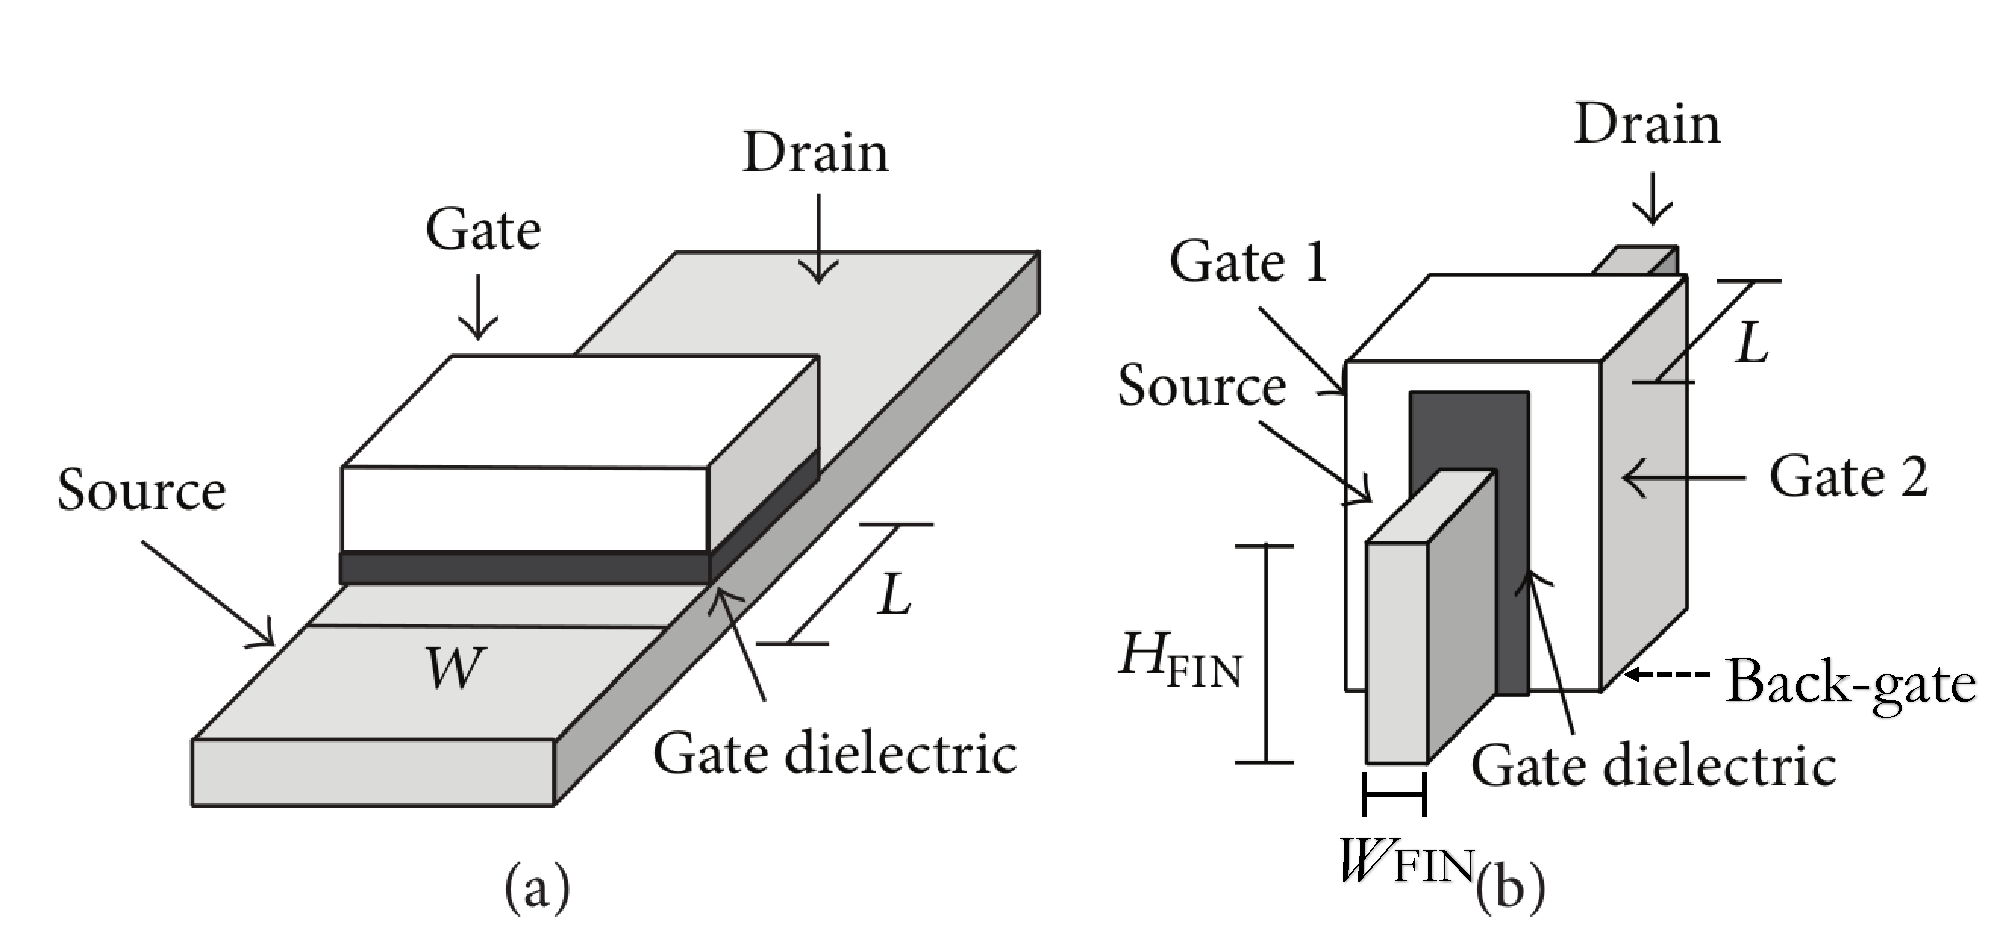
\includegraphics[width=0.8\textwidth, trim={0 0 0 0},clip]{finfet.pdf}
        \caption{Above, structural comparison between (a) planar MOSFET and (b) FinFET transistors. \\
		Below, structural comparison between (a) bulk and (b) SOI FinFETs.}
        %\label{mosfetvsfinfet}
        %\legend{Source: \citet{bhattacharya2014finfets}}
    %\end{figure}

    %\begin{figure} []
        \centering
        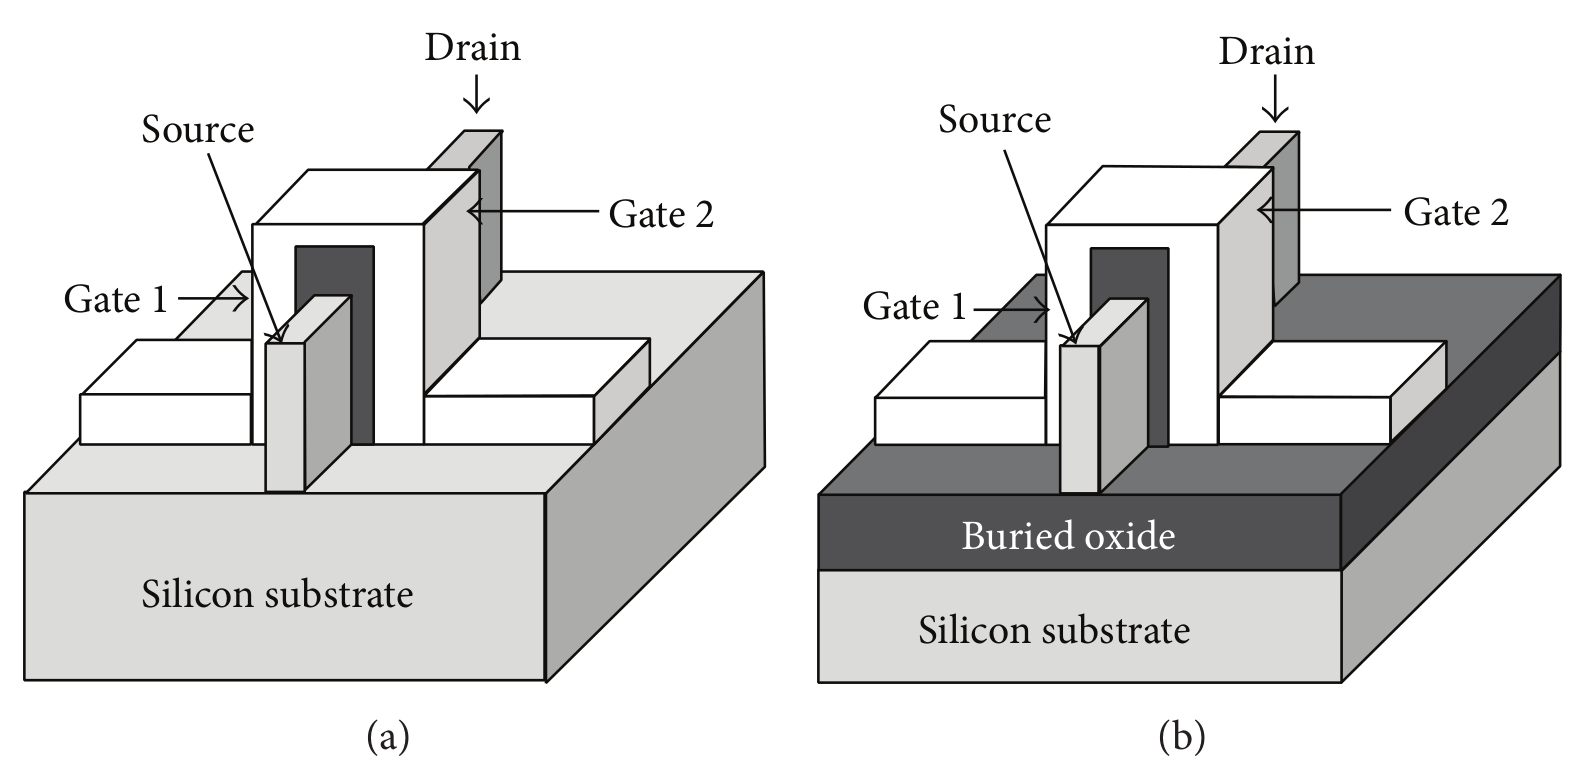
\includegraphics[width=0.8\textwidth, trim={0 0 0 0},clip]{finfet2.png}
        %\caption{Structural comparison between (a) bulk and (b) SOI FinFETs.}
        \label{finfet}
        \legend{Source: \citet{bhattacharya2014finfets}}
    \end{figure}

The channel being surrounded from three dimensions by the gate results in a superior control, reduced SCE and RDF effect due to the fully depleted channel that causes less sensitivity to process variations \cite{taur2013fundamentals}. FinFETs also present relative immunity to gate LER, a major source of variability in planar nanoscale FETs \cite{finfetchar1}. The disadvantage over bulk MOSFETs is the harder manufacturing process due to difficulty in the lithography steps as it is increasingly difficult to print small patterns, the increased variability impact due to the further miniaturization of dimensions, in comparison to bulk MOSFET and a more costly manufacturing process due to the need of techniques to address the manufacturing imprecision and, in the case of SOI FinFET, to change the CMOS substrate process to support a SOI substrate manufacturing process \cite{finfetchar1} \cite{finfetdis}.

Given the elevated levels of gate leakage due to the scaling down of the gate oxide, insulating materials with higher dielectric constant (high-k) have been introduced. Although, with the high-k dielectric adoption, challenges such as Fermi level pinning \cite{hobbs2004fermi} and phonon scattering \cite{gusev2006advanced} rised, being necessary the replacement of the traditional polysilicon gate electrode by a metal gate electrode \cite{gusev2001ultrathin, datta2003high}.

In the bulk FET devices in nanotechnologies, the variations in the gate length was the dominant parameter related to I\textsubscript{ON} deviations due to the RDF effects. Although, as a results of the shapes of the fin-like structures in FinFET, the channel is prefered to be low-doped in order to minimize threshold voltage variations. Given so, threshold voltage is mainly set by the workfunction.

Metals exist \textit{in natura} in the form of crystals where each atom has several bonds with adjacent atoms. Although, due to defects and disorientations, several crystals are formed, with "grain boundaries" between regions of regularity (crystal grains) in the metal \cite{dadgour2008statistical}, as shown in Fig. \ref{fig:meinMetalFab}. The electrostatic potential (e.g. $V_T$) varies depending on each grain boundary, as shown in Fig. \ref{WFFelectros}. At Table \ref{tab:WFForient} a example of possible orientation, probability and WF is given. Between several technology nodes - FD-SOI, Bulk and FinFET - the latter showed the lowest $V_T$ variation due to the much larger gate area \cite{dadgour2008statistical}.

\begin{figure} []
        \centering
	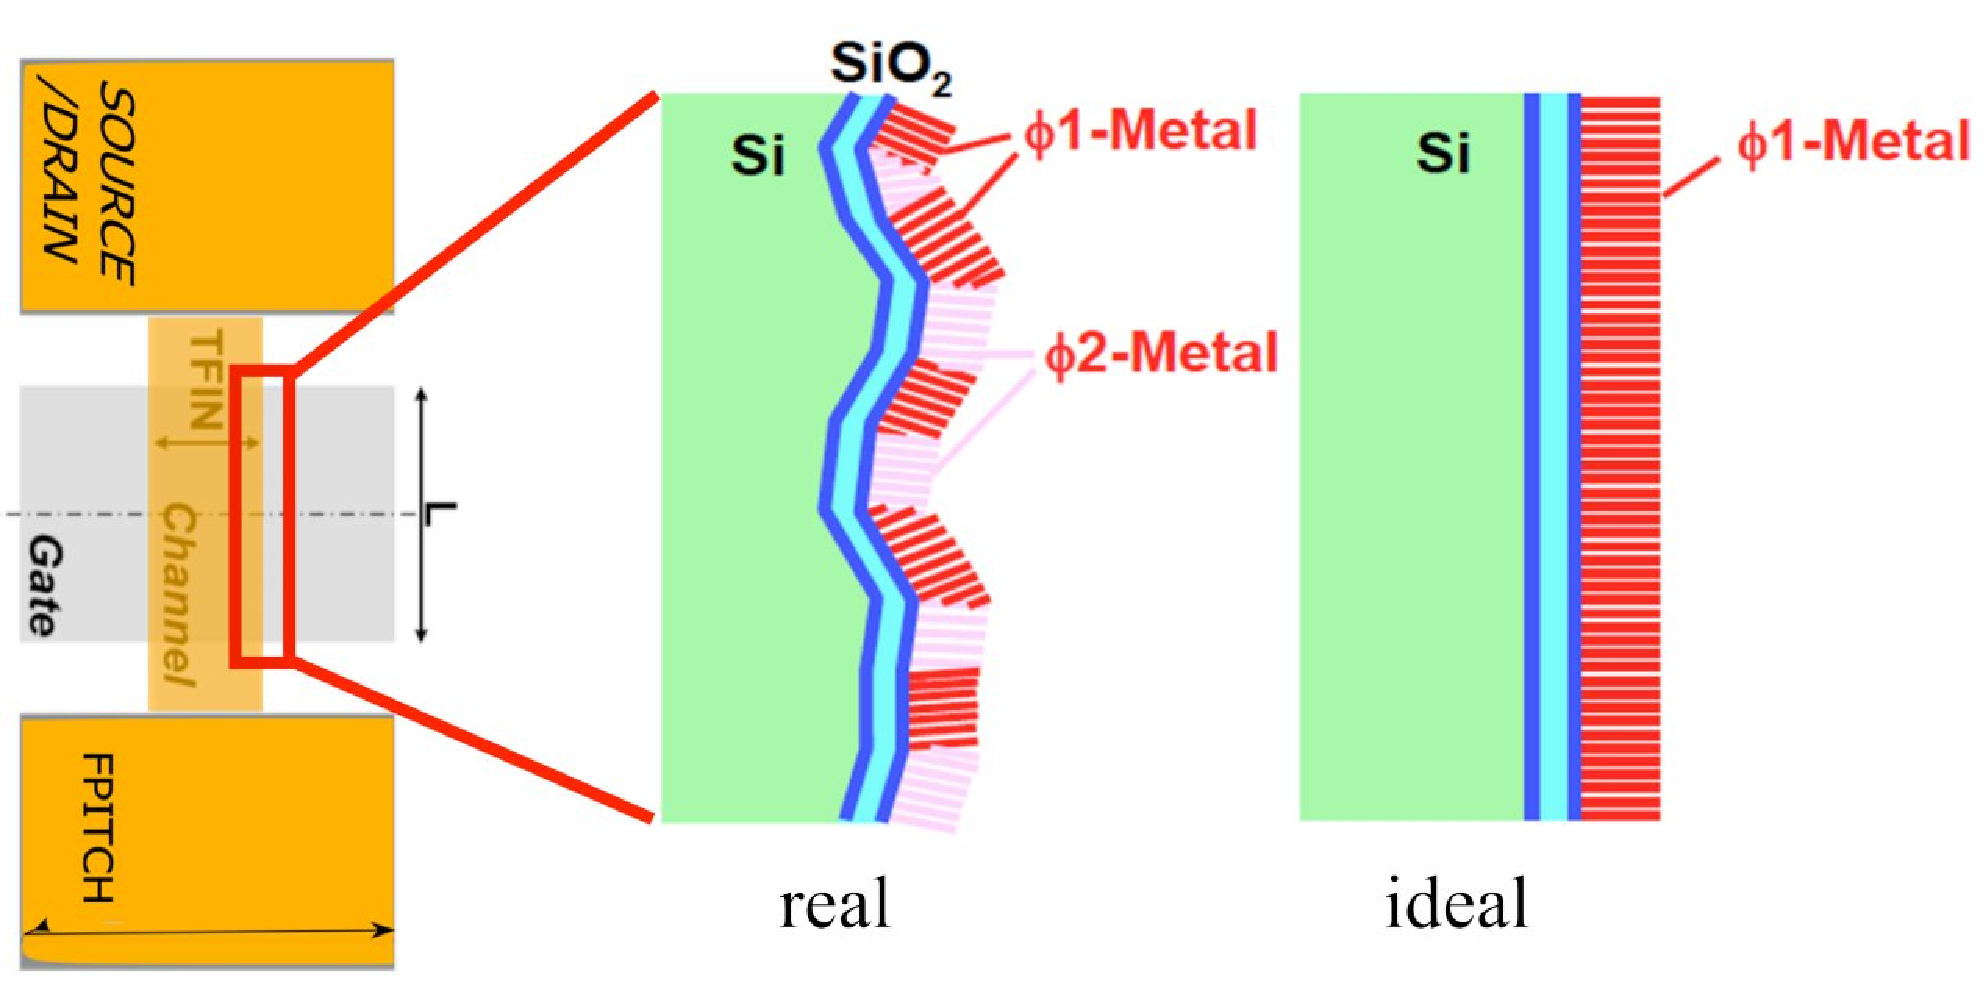
\includegraphics[width=0.75\textwidth, trim={0 0 0 0},clip]{chrome_2019-05-15_16-55-31.pdf}
        \caption{Metal fabrication ideal and real aspects.}
        \label{fig:meinMetalFab}
        \legend{Source: \citet{meinhardt2014impact}}
\end{figure}

\begin{figure} []
        \centering
        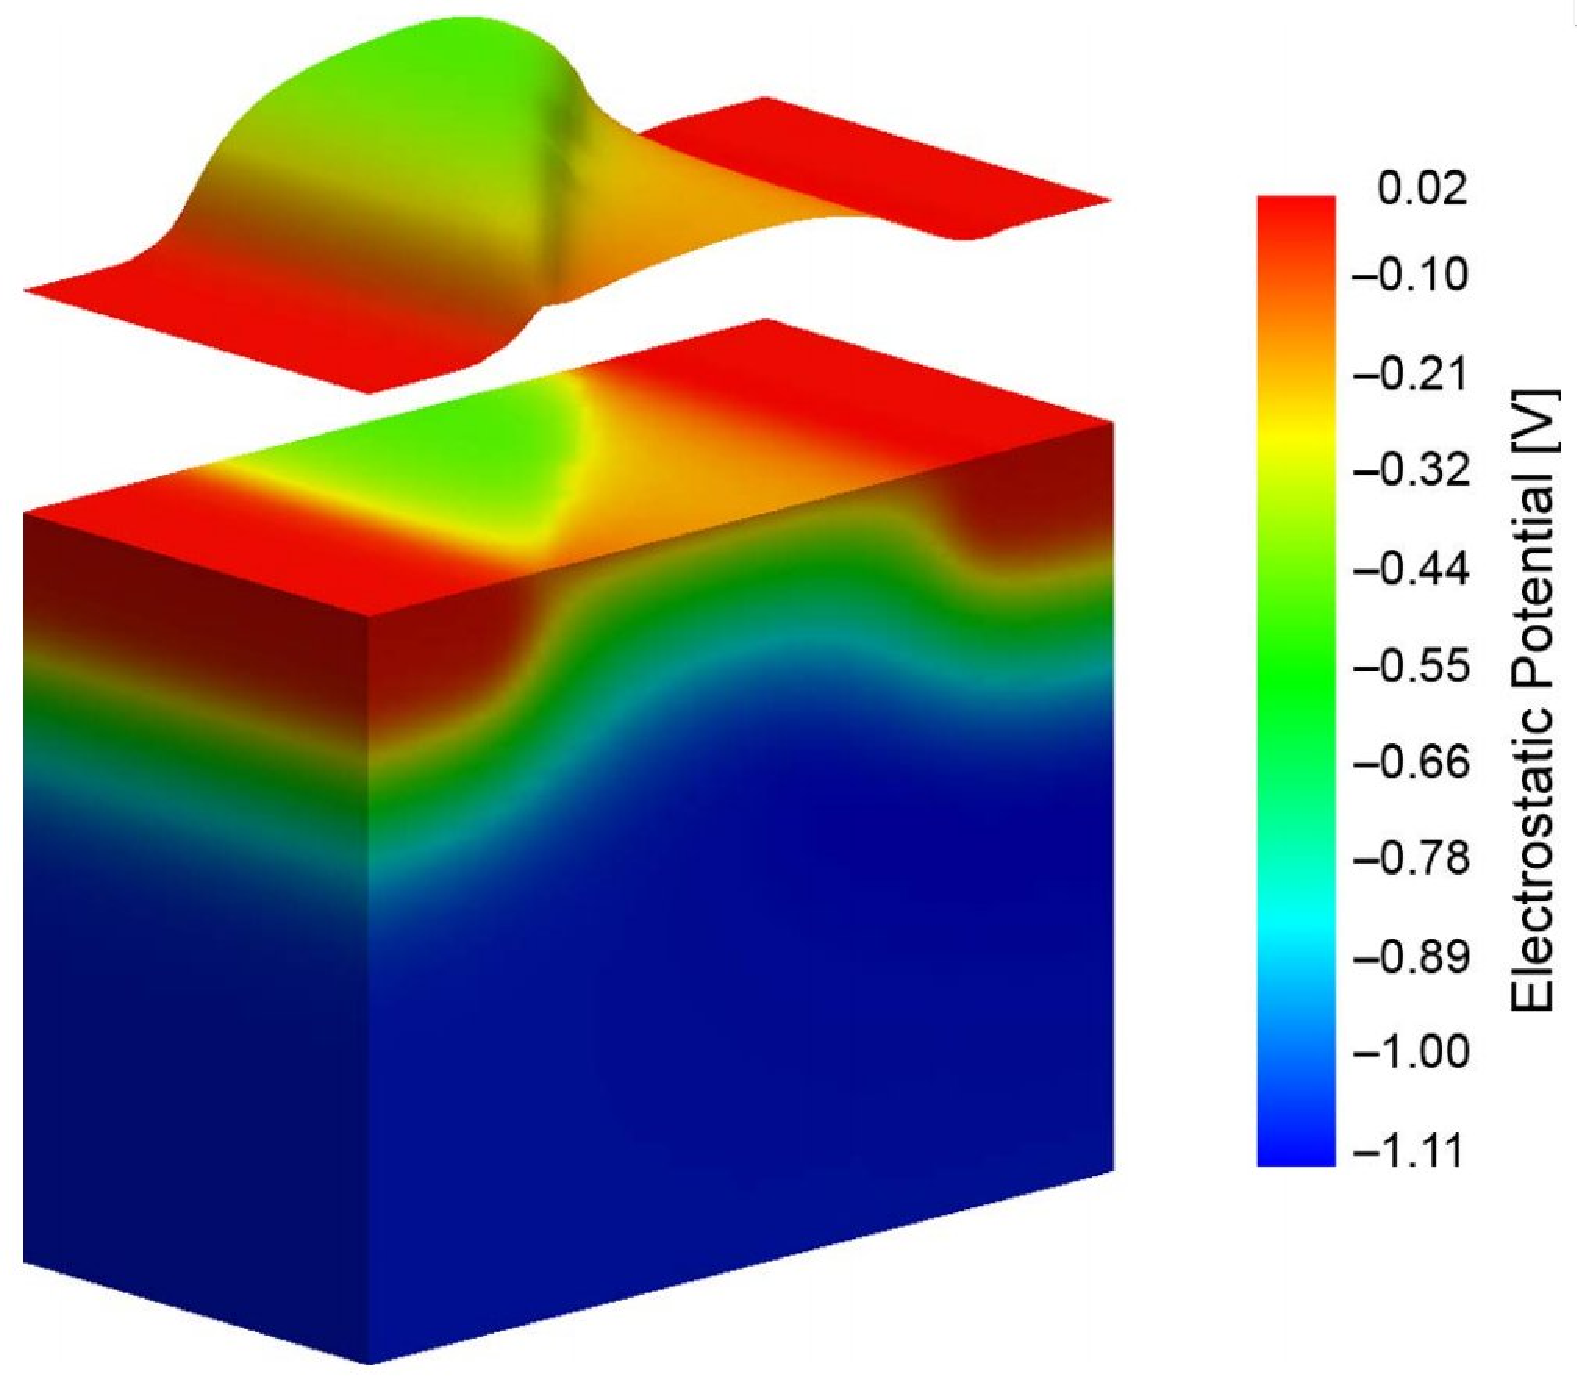
\includegraphics[width=0.5\textwidth, trim={0 0 0 0},clip]{pic-selected-190513-1743-08.pdf}
        \caption{Electrostatic potential in a generic 30-nm MOSFET with the surface potential shown below. The metal gate has two grains with the grain boundary diagonally across the channel.}
        \label{WFFelectros}
        \legend{Source: \citet{brown2010impact}}
\end{figure}

\begin{table}[]
\centering
\caption{}
\label{tab:WFForient}
\begin{tabular}{ccc}
\hline
\textbf{Orientation}                  & \textbf{Probability} & \textbf{Work Function} \\ \hline
\textbf{\textless{}200\textgreater{}} & 60\%                 & 4.6 eV                 \\ \hline
\textbf{\textless{}111\textgreater{}} & 40\%                 & 4.4 eV                 \\ \hline
\end{tabular}
\legend{Source: \citet{brown2010impact}}
\end{table}

The WFF impact can be better understood when considering the equation \ref{eqn:wffvt}, where the threshold voltage for multigate devices is expressed. Additionally, the fermi potential for the P-type silicon is given by equation \ref{eqn:ff} \cite{colinge2008finfets}.

The effects of $Q_D$ and $Q_{SS}$ onto the threshold voltage ($V_{th}$) are almost negligible compared to $f_f$, in ultrathin body and lighly doped devices, like the FinFET. Additionally, $V_{in}$ is the additional surface potential to $2f_f$, of ultrathin body devices, that is needed to accumulate enough inversion charges into the channel region of the transistor to reach the threshold point \cite{mustafa2013threshold}.

    \begin{equation}
        \centering
        \label{eqn:wffvt}
        V_{th} = f_{ms} + 2f_{f} + \frac{Q_D}{C_{ox}} - \frac{Q_{SS}}{C_{ox}} + V_{in}
    \end{equation}
where:
\begin{conditions}
Q_{SS} & charge in the gate dielectric \\
C_{ox} & gate capacitance \\
Q_{D} & depletion charge in the channel \\
f_{ms} & work-function difference between the gate electrode and the semiconductor \\
f_{f} & fermi-potential
\end{conditions}
    \begin{equation}
        \centering
        \label{eqn:ff}
        f_{f} = \frac{kT}{q} ln\frac{N_A}{n_i}
    \end{equation}
where:
\begin{conditions}
N_{A} & acceptor concentration \\
n_{i} & intrinsic carrier concentration \\
\end{conditions}
Several works analyze the FinFET reliability. It is shown in \cite{meinhardt2014impact} the major influence that WF Fluctuations (WFF) exercise over $V_{T}$ variations of several standard cells. In addition, in \cite{wang2011statistical} it was shown the high correlation between the $I_{ON}$ and $I_{OFF}$ currents and $V_T$ fluctuations due to the granularity of the metal gate.

In \cite{FinFET04} the modeling of the reliability degradation of a FinFET-based Static Random Access Memory (SRAM) is shown. It is concluded that the probability of failure due to NBTI and Gate Oxide Break Down (GOBD) is relatively lower in comparison to HCI-induced failures. They also shown the improvement of lifetime due to Error-Correcting Code (ECC) memory.

In \cite{FinFET01} it is shown, at 14/16nm fabricated bulk FinFET technology, that for high energy charged particles, the drive current is the dominant factor to the transient fault pulse width and cross-section. And low energy particles have a grater dependence on secondary transistor and circuit design factors (number of fins, transistor arrangement, etc).

In \cite{FinFET02} the HCI effect is analyzed in pass-gate FinFET transistors. The tests were executed using a commercial FinFET technology showing a 50\% chance of errors due to HCI in pass-gate transistors. In \cite{FinFET03} a analysis of the sensitivity of double-gate and FinFET devices to process variations is shown. It is concluded that for 20nm FinFET devices large channel doping concentration is necessary to obtain suitable values of $V_T$ if heavily doped polysilicon gates are used. Due to the small volume of the channel doping will bring unacceptable $V_T$ fluctuations. Given that, heavily doped polysilicon may not be a viable choice with the work function adjustment being a better approach.

 In \cite{FINFET05} an investigation on reliability characteristics of NMOS and PMOS FinFETs is conducted. Based on fabricated FinFETs transistor with 17-27 nm width, it was shown that the life-time of FinFET is very dependable of its dimensions. The predicted lifetime for a 50nm gate length NMOS FinFET was 133 years, for the first HCI event. While a 27nm fin-width PMOS FinFET showed 26.84 years of lifetime wich is reduced to 2.76 years when reducing its fin-width from 27 to 17 nm for a NBTI event, showing the huge reliability challenge introduced by technology scaling.

Given all the works trying to characterize the impact of variability in FinFET devices, and developing methods to tackle this problem, at several levels of abstraction, the FinFET variability challenge is kept as an open problem. This work aims to assess whether there are inverter circuits applicable for replacing the traditional inverter, presenting better results in relation to the impact of process variability, while maintaining low energy consumption.


\chapter{Considered Designs To Cope With Variability}

This work selected 4 inverter alternative circuits based in recent literature, in order to evaluate their effectiveness in diminishing the impact of variability into metrics.

Schmitt Triggers are commonly used as internal circuits on systems to provide enhanced noise tolerance and robustness against random variations in the input waveforms. On a typical input (non-ST), its binary value will switch at the same point on the rising and falling edges. With a slow rising edge, the input will change near the threshold point. When the switching occurs, it will require current from the supply source. With current being pushed from the supply, it can cause a voltage drop across the circuit causing a shift in the threshold voltage.

If the threshold shifts, it will cross the input causing it to switch again. It can go indefinitely causing oscillation. The same thing can happen if there is noise on the input. STs are applied in these cases to filter noise introducing superior and inferior threshold voltages. STs circuits present a hysteresis characteristic. This hysteresis exists in the presence of two switching $V_T$. If the input level is within the hysteresis region, the ST shall not switch. Such characteristic gives a higher static noise margin (SNM) in comparison to traditional inverters, ensuring a high noise immunity.

 Variations in physical parameters became alarming at ultra-deep sub-micron (UDSM) nodes because the node scaling was accompanied by a supply voltage scaling, making the circuits more susceptible to noise and electromagnetic interference due to the deterioration in SNM \cite{pal2018circuit}. Given that, this work explores four types of inverters, where three of them are considered STs given their hysteresis characteristic.

 \section{ST Topologies and alternatives}

A variety of CMOS STs have been proposed and implemented over the years based on different requirements. A higher performance ST is proposed in \cite{steyaert1986novel} where, by a different design, a smaller load capacitor value is achieved, decreasing the slew rate of the ST internal node. In \cite{pfister1992novel} a ST with a programmable hysteresis is proposed. The programmable hysteresis is achieved by adding a P and N transistors in series with the 6T ST $P_F$ and $N_F$ transistors, respectively, both receiving the same gate signal. \cite{kim1993new} proposes a 10T ST which its hysteresis interval does not depend on transistors width/length ratios being, consequently, more robust to process variations.

 A low-power ST is proposed at \cite{al2002low} with low short circuit current achieved by the presence of only one path to each power rail, being recommended for low power, and very low frequency applications. In \cite{pedroni2005low} proposes a low-power ST by having only one transistor transmitting (at stable output values), considerably reducing power consumption. STs can be optimised by adequate dimensioning as well as stated in \cite{tache2018reliability} where the OTS technique presented the best metrics for low power applications, in accordance to \cite{zimpeck2016finfet}.

In \cite{shah2020soft} a voltage-booster is applied in the traditional 6T ST in order to replace its pull up network and reduce the number of PMOS transistor to only one. This replacement makes it less vulnerable to the effects of NBTI, which severely affects PMOS devices. It was simulated on 32 nm bulk CMOS technology and was revealed to present an almost negligible delay shift of 0.47\%, with the traditional 6T ST and CMOS inverter presenting 7.2\% and 5.32\% shifts, after three years of simulated NBTI stress, respectively. Furthermore, it presented an improved sensitivity against charged particles of 62.48\% and 55.10\% against the CMOS inverter and 6T ST, respectively. And finally, it presented 168.68\% less deviations in comparison to the CMOS inverter considering process variability. It is important, though, to highlight its 4.315x higher leakage power and potential higher area, given finfet technology restrictions considering the higher number of NMOS transistors (5) in comparison to the traditional 6T ST (3).

In \cite{dokania2015circuit} a novel technique based on the replacement of FA’s internal inverters with low voltage STs for PVT variability robustness improvement is originally introduced and applied on seven different FA designs. The simulations were performed using the 16nm bulk CMOS predictive technology model in SPICE. It presented significant variability improvement up to 4.8x in PDP. Although, the improvements occur at the cost of an increase in the area and power dissipation of each design. This technique is tested in several works: in \cite{samuel2016} the ST technique is applied on four FAs. It presented promising results regarding the power deviation due to the process variability with a decrease up to 79\% with a drawback of a significant increase in average energy consumption. The simulations were performed with the 16nm technology predictive technology model in SPICE.

 In \cite{ahmad2016single} it is presented a novel Schmitt-trigger-based single-ended 11 Transistor SRAM cell. It analyses its performance against seven different SRAM topologies. The novel cell showed the least energy consumption per operation with the smallest leakage power and a 6.9x higher $I_{ON}$/$I_{OFF}$ ratio. Further PVT variability simulations confirmed the robustness of the design regarding read and write operation. The simulations were carried in 22nm predictive technology using SPICE. \cite{moghaddam2017design} presents a ST buffer using CNFET. It was evaluated against other two buffers and showed, on average, 68\% higher critical charge and 53\% lower energy consumption and a huge gain considering PVT variability robustness. The simulations were carried in 16nm Stanford CNFET model using SPICE. Lastly, in our previous work \cite{moraes2018evaluation}, the ST technique is evaluated considering 4 different FAs layouts at 7nm FinFET. 64.74\% and 66.6\% reduction in delay and power deviation was achieved.

\section{Evaluated Circuits}

Several circuits were chosen to be analyzed as alternatives to mitigate the effects of process variability. Simulations considering several supply voltage levels, transistor sizing, and level of process variability will be carried out upon the considered designs, and their results are compared, in order to indicate the most appropriate design for each type of application and priority. The following circuits are considered:


\subsection{Traditional 6T ST}
The 6T traditional ST main feature is the presence of ${P_F}$ and ${N_F}$ devices as shown in Fig. \ref{fig:ST} \cite{doki1984cmos}. These transistors are responsible for a feedback system. For example, if the output is in a high level, the ${N_F}$ is on, pulling the node ${X}$ to a high potential, and forcing the drain-source voltage of transistor ${N_I}$ almost zero and its gate-source voltage into the negative region. This kind of arrangement reduces the leakage current ${N_I}$ exponentially, increasing the on-to-off current ratio, and minimizing the output degradation \cite{lotze2017ultra}.

The main effect of process variability is a shift on the voltage transfer curve (VTC) due to the threshold voltage variation. Usually, the input voltage, where a device starts delivering current, is directly dependent on the $V_T$. Thus, the variability impact on VTC is reduced in the ST as a result of the high influence of the gate-source voltage of the inner transistor ($N_I$ and $P_I$) over its switching point \cite{lotze2017ultra}.

\begin{figure}[]
  \centering
    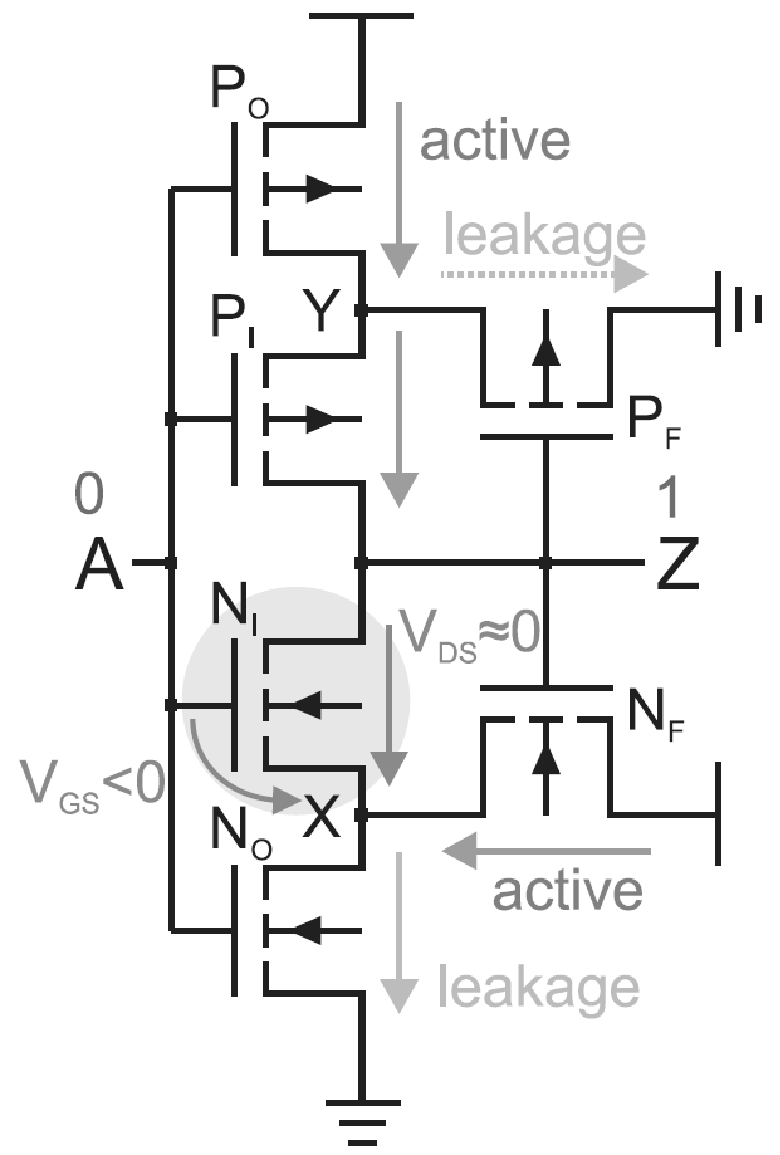
\includegraphics[width=0.3\textwidth]{ST.pdf}
     \caption{ST inverter leakage suppression \cite{lotze2017ultra}.}
  \label{fig:ST}
\end{figure}

The 6T ST was chosen due to promising results at \cite{lotze2017ultra}, where a ST-based 8x8 multiplier was presented, with the ST greatly improving the on-to-off current ratio. In \cite{kulkarni2007160} a SRAM based on 6T ST is proposed working at 160mV and showing improvements of both robustness and static noise margins in comparison to a traditional inverter-based solution.

\subsection{Three Inverter Schmitt Trigger (TIST)}

The TIST, shown in Fig. \ref{fig:TIST} is a ST implementation, most common in textbooks. It has been mostly unexplored for low power applications. It consists of a CMOS inverter followed by a latch. The idea behind this circuit is related to the switching threshold of a CMOS inverter being determined by the ratio between NMOS and PMOS transistors ($k_n$/$k_p$). Increasing the ratio results in a reduction of the threshold and vice-versa. Adapting the ratio depending upon the direction of the transition results in a shift in the switching threshold, characterizing a hysteresis effect. This effect is achieved with a feed-back mechanism, as the previous design. For example, when the input signal is low (zero) the $P2$ and $P0$ are conducting, while the $N2$ and $N0$ are off.

As the input goes high (one) with $P1$ shutting down and $N1$ start conducting. As the input to the latch start discharging $P2$ and $P0$ will start conducting at the same time, changing the ratio between the number of parallel PMOS/NMOS transistor conducting and effectively changing the ratio. The same dynamic occurs when changing the input from a high value to a low value, just inverting the transistors from PMOS to NMOS and vice-versa. The brief ratio change is enough for decreasing the switching threshold for the appearance of hysteresis. The TIST in this work has been modified in order to turn it into an inverter. The original TIST is shown in \cite{rabaey2002digital}.

\begin{figure}[t]
  \centering
    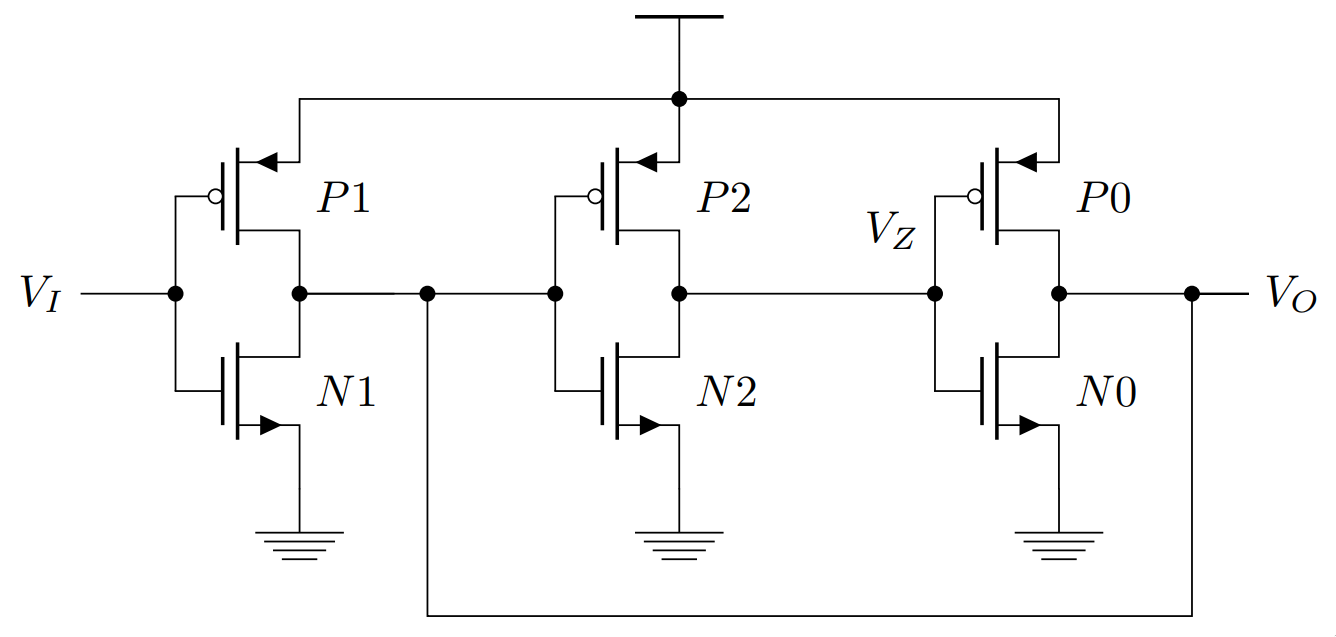
\includegraphics[width=0.8\textwidth, trim={0cm 0cm 0cm 0cm}, clip]{TIST.png}
     \caption{Modified TIST schematic \cite{rabaey2002digital}}
  \label{fig:TIST}
\end{figure}

According to \cite{thiagoTIST}, the TIST is able to provide hysteresis from a supply voltage as low as the classical inverter unity gain. However, for higher supply voltages, the hysteresis interval will grow excessively to a point where the cell locks itself in a random state (low or high), which cannot be changed. Futhermore, it was shown that the hysteresis interval and the minimum supply voltage for it to appear greatly benefit from increasing the ratio between the latch and inverter transistors. Given so, in order to tackle some of that problem, the inverter transistors were sized with a higher number of fins in comparison to the latch. Still, it shows the TIST viability to work at sub 100mV supply voltages, which will be explored in future works.

\subsection{Stacked Inverter Gate (SIG)}

SIG, shown in Fig. \ref{fig:SIG}, is a circuit composed of unbalanced inverters without positive feedback, referred to as stacked, or redundant, inverters. It presented improvements over the CMOS inverter regarding voltage gains \cite{bose2018stacked, luo2017sub}. Originally, it was applied on replacing the inverter of a ring-oscillator working at a sub-50mV supply voltage, presenting 30\% higher gains, claiming that energy harvesting techniques based on the body-to-ambient temperature gradient can leverage such oscillator to achieve self-startup.

\begin{figure}[]
  \centering
    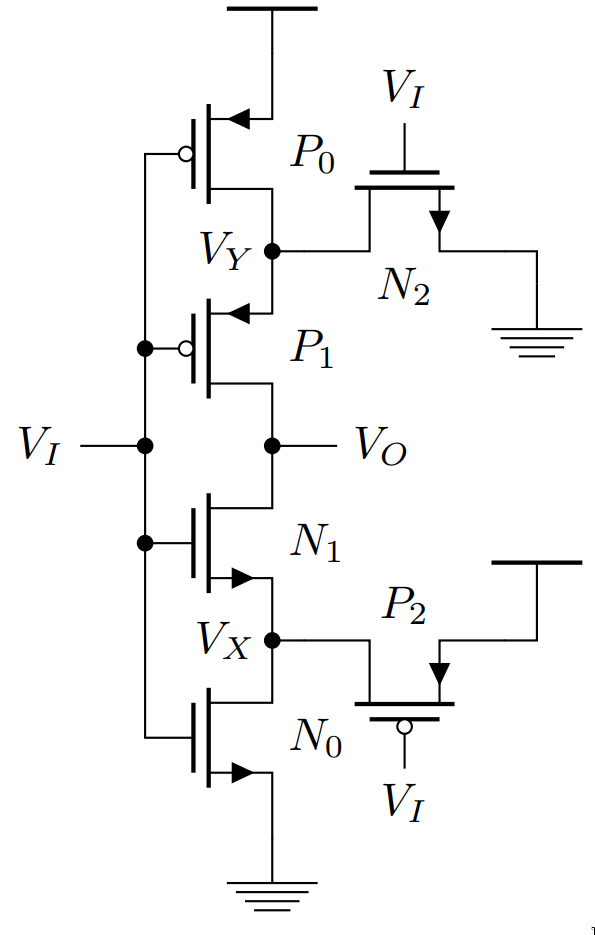
\includegraphics[width=0.3\textwidth]{SIG.png}
     \caption{SIG schematic \cite{bose2018stacked}}
  \label{fig:SIG}
\end{figure}


\subsection{Low Power Schmitt Trigger (LPST)}

The following circuit is not compared to the previous ones, although being applied on the following analysis considering the replacement of FAs internal inverters. It was not applied in the comparison between inverter circuits due to technology restrictions, which did not permit to connect the NMOS devices back-gates to specific nodes. The LPST inverter circuit used in this work was inspired by \cite{zhang2003low} and modified in \cite{dokania2015circuit} to achieve the desired inverting characteristic, as shown in Figure \ref{fig:LPST}.

\begin{figure}[h]
  \centering
  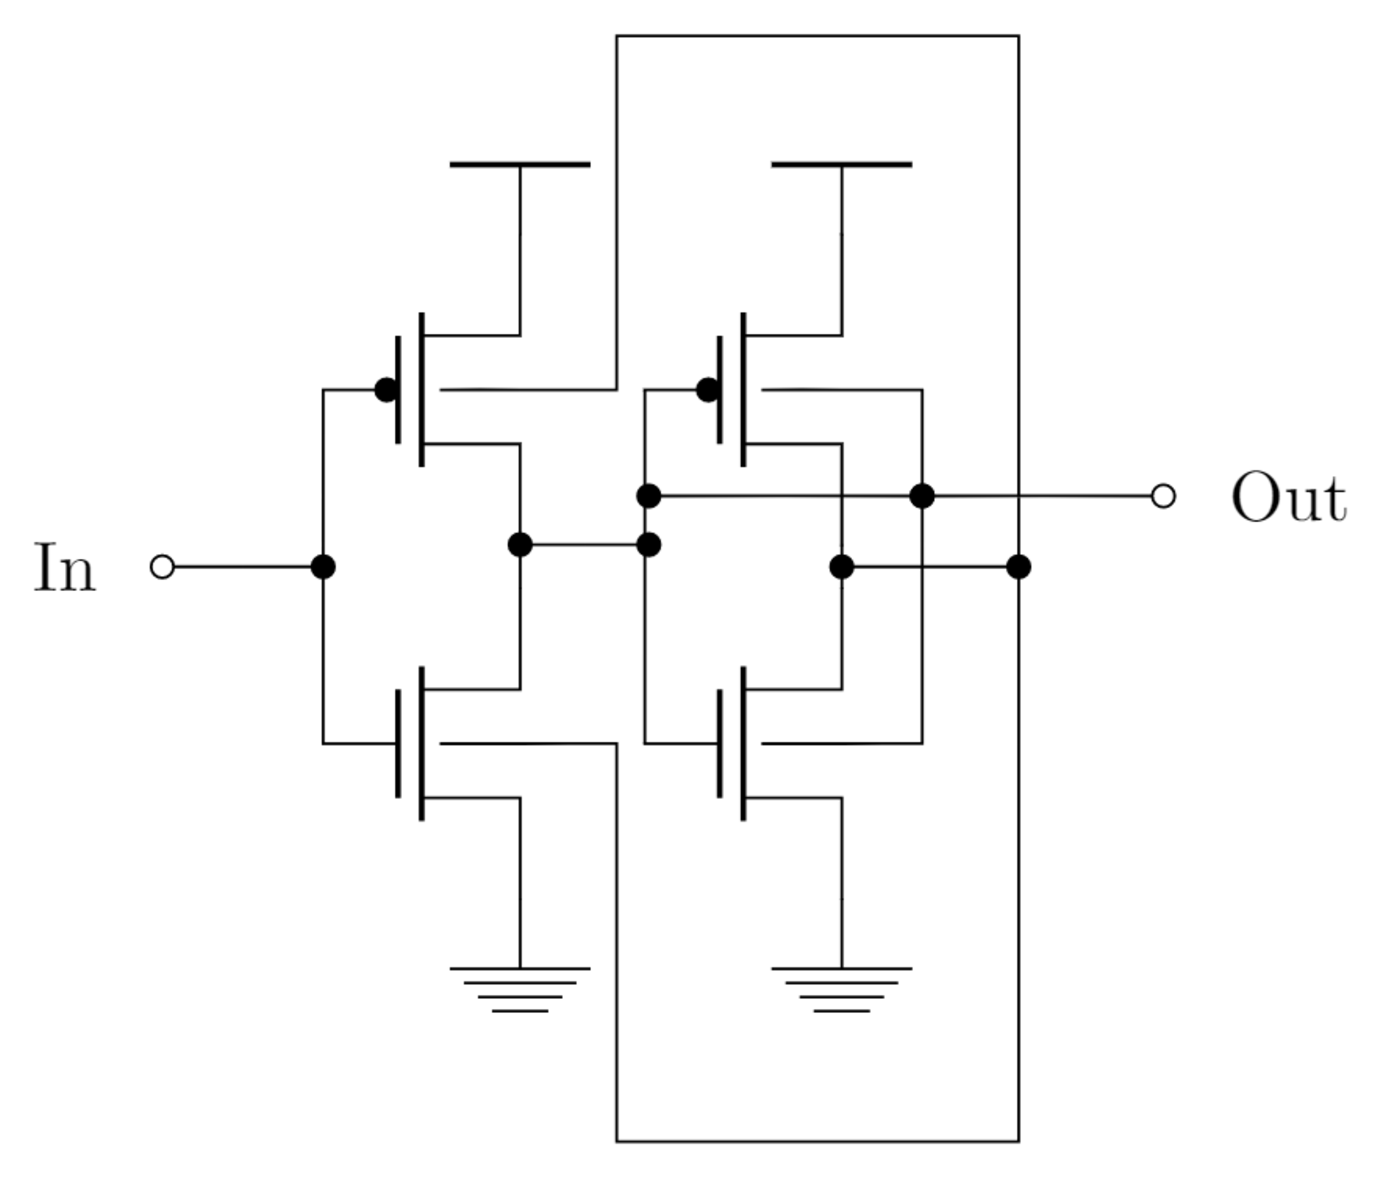
\includegraphics[width=.5\linewidth]{STOriginal.eps}
  \caption{LPST Inverter from \citet{dokania2015circuit}}
  \label{fig:LPST}
\end{figure}

It is designed for operation at a supply voltage of 0.4V in order to achieve low power consumption, and consists of the junction of two inverters where the output from the second one will be the bulk for the first one. On previous work \cite{moraes2018evaluation}, the LPST was applied on Full Adders, presenting up to 37.38\% decrease on energy deviations at nominal level supply voltage and 66.59\% for near-threshold operation (0.4V). In this design a dynamic body-bias technique is applied through a feedback mechanism to a standard CMOS inverter circuit, thus allowing a change in the threshold voltages of two MOSFETs, implying a change in the switching voltage. In order to provide an overview, the number of transistor and main characteristic for each design are highlighted at Table \ref{tab:designHighlight}.

\begin{table}[]
\centering
\caption{Each design number of transistors and main charactereristic, advertised by respective works.}
\label{tab:designHighlight}
%\resizebox{\textwidth}{!}
\end{table}

%\begin{figure}[]
%\centering
%\begin{subfigure}{.5\textwidth}
%  \centering
%  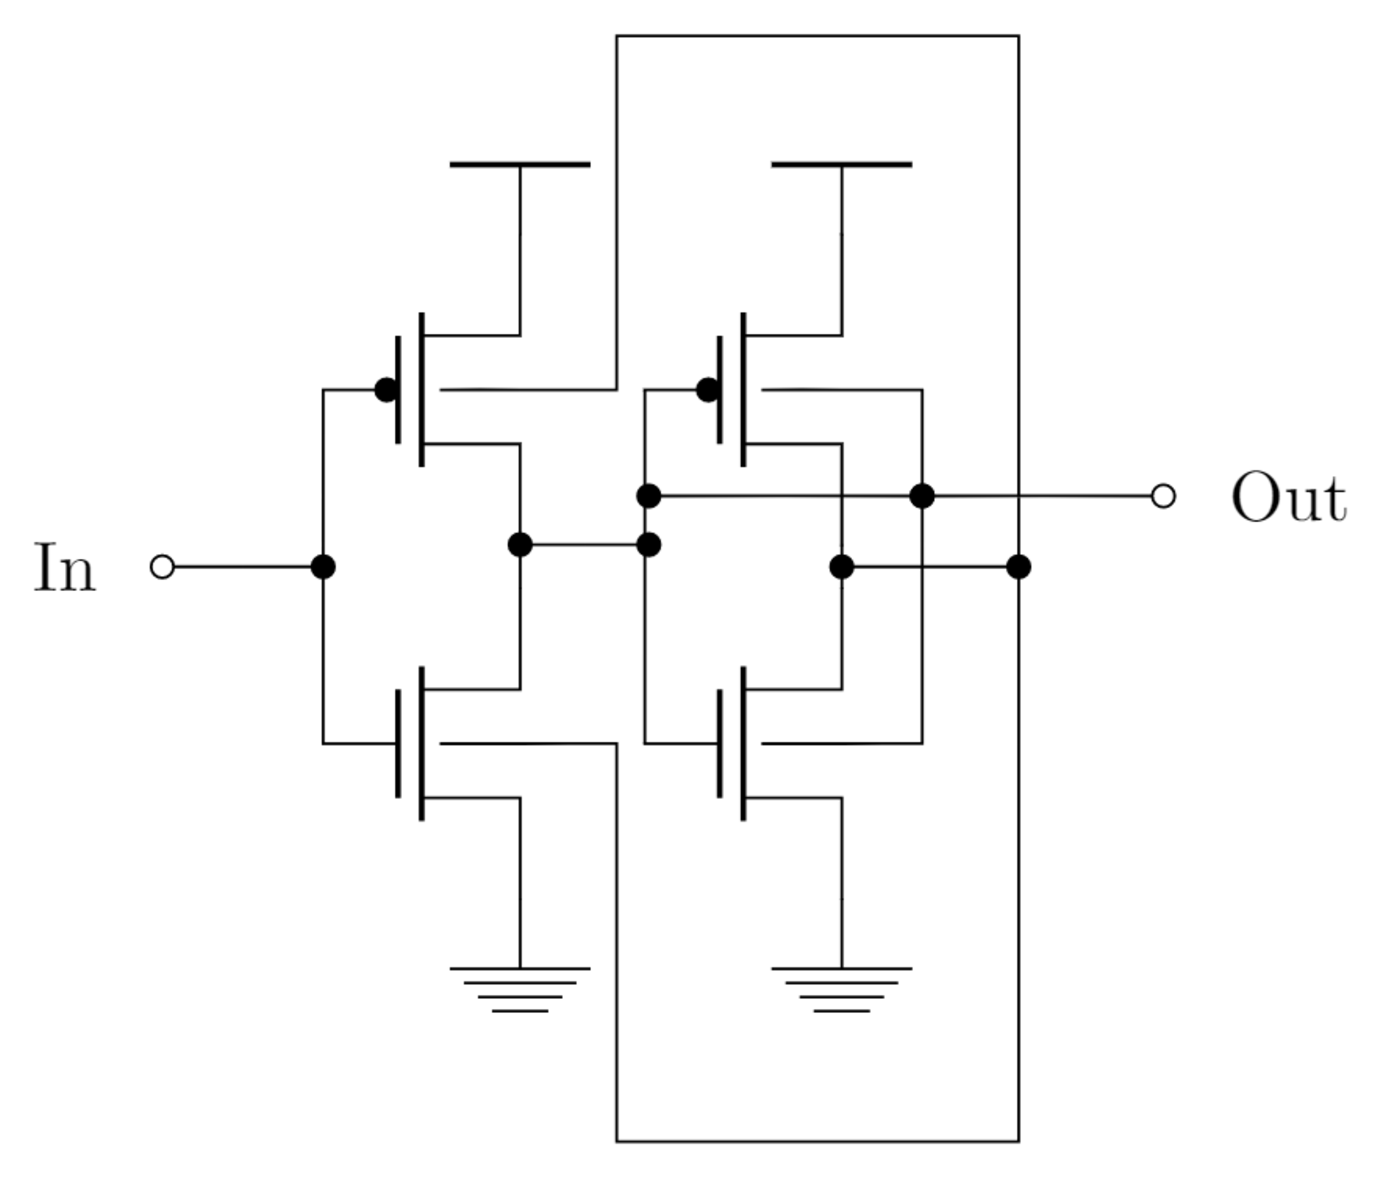
\includegraphics[width=.8\linewidth]{STOriginal.eps}
%  \caption{LPST Inverter from \citet{dokania2015circuit}}
%  \label{fig:sub1}
%\end{subfigure}%
%\begin{subfigure}{.5\textwidth}
%  \centering
%  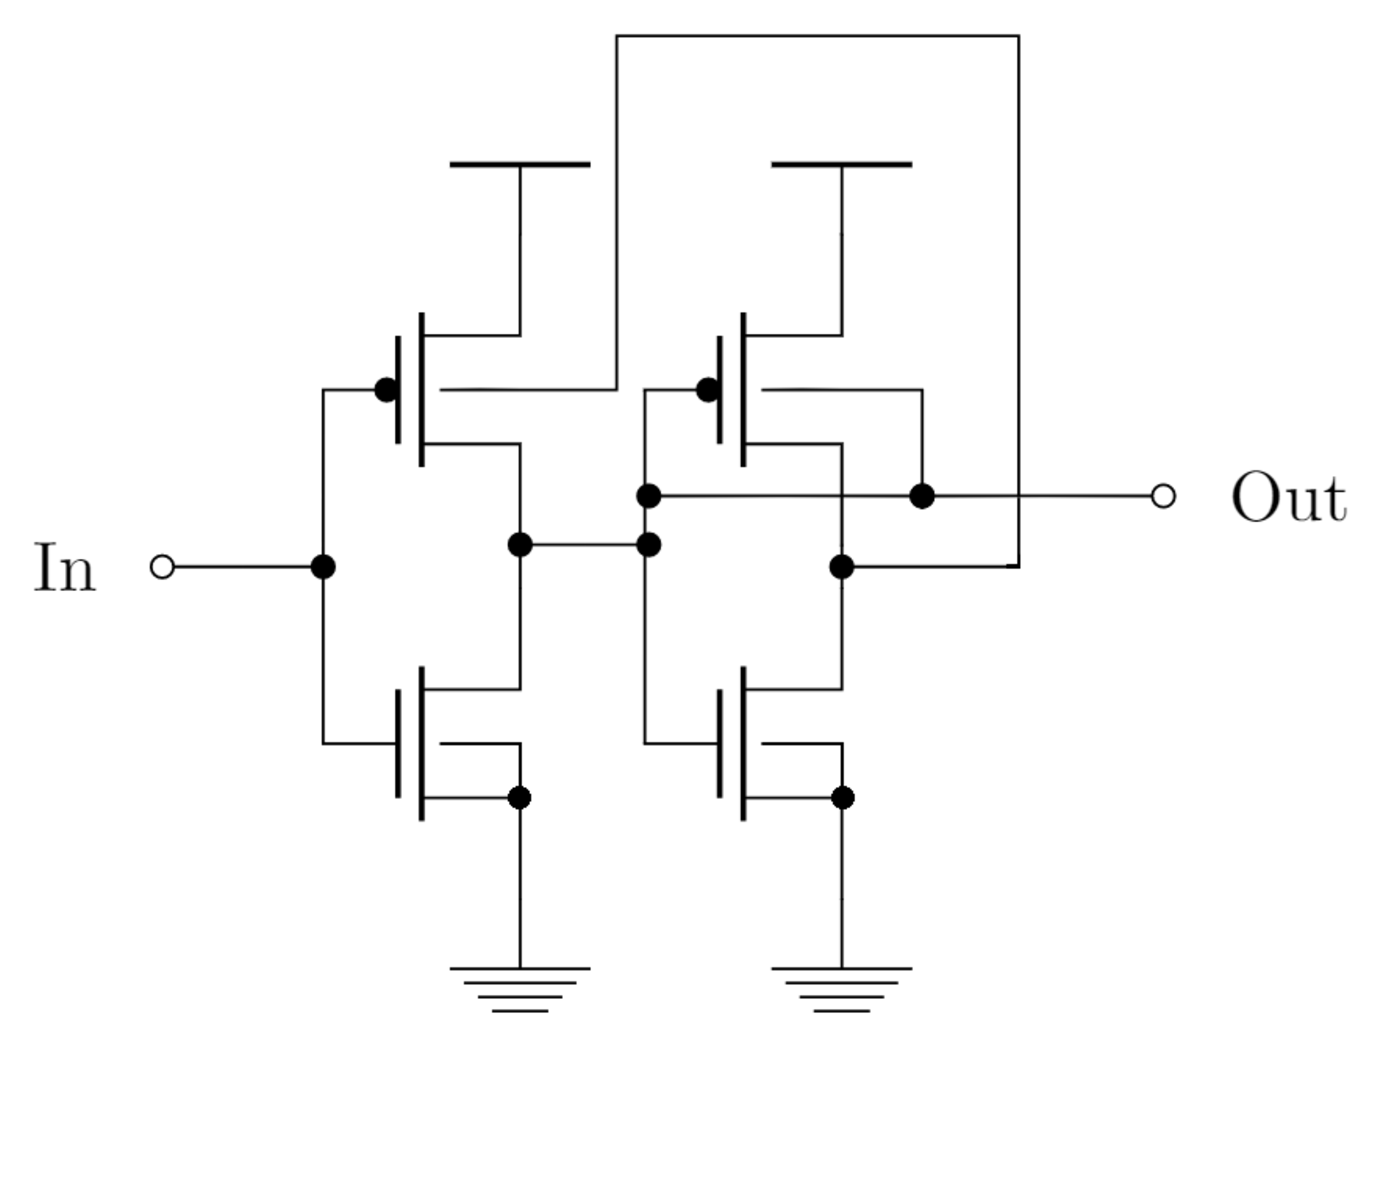
\includegraphics[width=.8\linewidth]{STcorrigido.eps}
%  \caption{Modified LPST Inverter applied in this work. Source: From the author.}
%  \label{fig:sub2}
%\end{subfigure}
%\caption{Original and modified Low Power STs (LPST) side-by-side}
%\label{fig:test}
%\end{figure}

%\chapter{Objectives}

%Given the laid concepts, this work has two objectives. The first is to identify an appropriate layout, considering the number of fins, and supply voltage in order to achieve a minimum energy device. The considered circuits will be the traditional 6T ST, SIG, TIST and, for the sake of comparison, a traditional inverter. Multiple levels of process variability will be considered. Therefore, depending on manufacturability quality, different recommended layouts and supply voltages can arise. There will be considered the means, standard deviations and normalized standard deviations for each metric, energy, delays on and off currents, current ratios and hysteresis interval (when applicable), respectively.

%While, the second objective is to apply the ST technique into FAs, in the case, the CMOS, TFA, TGA and Hybrid FAs. The two ST applied are the traditional 6T ST and the low-power back-gating-based ST from \cite{zhang2003low}. The technique consists of the replacement of the FAs internal inverters with the respective STs. All layouts will be designs with a fixed number of transistors and two levels of supply voltages. All simulations will be performed at the same level of process variability. There will be considered the means, standard deviations and normalized standard deviations for each metric, energy and delays, respectively.

\chapter{Methodology}

To provide an extensive exploration of the process variability effects on the circuits characteristics, this work evaluates:

1) 4 inverter circuits. The traditional CMOS inverter, the 6T ST, the SIG, and TIST, operating at multiple combinations of supply voltages. The supply voltage range will start from 0.1V to 0.7V (nominal) in 100mV steps;

2) the influence of the transistor sizing where all transistors have the same number of fins (except for the TIST), ranging from 1 fin to 5 fins, increasing the number of fins one-by-one;

3) the impact of these parameters on the maximum achievable frequency within a failure threshold of 10\% of the 2000 Monte Carlo simulations;

4) the impact of different levels of process variability (WFF) from 1\% to 5\% in steps of 1\%. This variations is inserted into the simulations following gaussian distribution;

5) as a case-study to show the potential of these circuits as a technique to mitigate process variability effects.

The design flow is shown at Figure \ref{DesignFlow}. The design was divided into two main steps: the layout design and electrical simulations. After finishing the layout design process, each layout passed through validation which consisted of a Design Rule Checking (DRC) to detect if the layout obeys the technology geometry restrictions and layer rules, Layout Versus Schematic (LVS) where the schematic and the layout extracted netlists are compared to detect their equivalence (same nodes and nets) and a Behavioral test, to observe if the circuit works as expected.

\begin{figure}[]
\centering
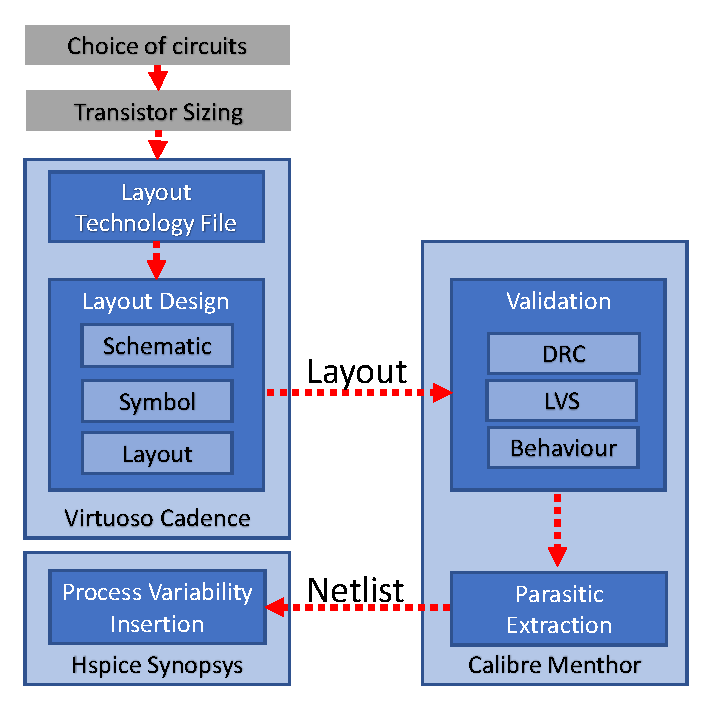
\includegraphics[width=0.6\textwidth, trim={0.25cm 16cm 3cm 0.5cm},clip]{designFlow.pdf}
\caption{Design flow of the experiments.}
\label{DesignFlow}
\legend{Source: From the author.}
\end{figure}

The transistor sizing exploration evaluate layouts from 1 to 5 fins through 1-fin steps for the CMOS inverter, the traditional ST and the SIG. The TIST did not present an adequate behaviour with its P and N devices presenting the same number of fins, with its output value getting stuck. Thus, for the TIST, a different approach was adopted. The TIST consists of a traditional inverter (transistors $P_1$ and $N_1$) followed by a latch (transistors $P_0$, $P_2$, $N_0$ and $N_2$), given so, the inverter transistors were resized following a proportion between their size and the size of the latch transistors. It was adopted two proportions: 2:1 and 3:1, resulting in five different layouts. Three layouts follow a 2:1 proportion with the inverter transistors containing 2, 4, and 6 fins and the latch transistors containing 1, 2, and 3 fins, respectively. Two layouts follow a 3:1 proportion with the ST transistors containing 3 and 6 fins, and the latch transistors containing 1 and 2 fins, respectively. For the sake of simplicity TIST layouts will be refered to as TIST2F1F, TIST4F2F, TIST6F3F, TIST3F1F and TIST6F2F. With such sizing, the TIST worked properly in a higher number of cases, with near-threshold voltage operations presenting the highest number of failures.


\section{Layout Design}

All circuits were designed using the Virtuoso Electronic Design Automation (EDA) tool from Cadence\textregistered with the process design kit (PDK) of 7-nm FinFET of Arizona State Predictive PDK (ASAP7) from the Arizona State University in partnership with ARM \cite{clark2016asap7}. It is the only open-source and free 7-nm PDK available for academic use. This PDK was chosen due to realistic design conjecture regarding the current design competencies. FinFET technologies present the width quantization aspect \cite{2000Simulations}. With a 27nm fin pitch, high-density layout is achieved with 3-fins transistors. Otherwise, for a higher fin count, there is a lower density and routing complexity \cite{chava2015standard}. The main PDK rules and lithography assumptions considered in this work are shown in Table I. To exemplify the PDK layers, the 3-fins transistors ST is shown in Fig. \ref{fig:layers}. The dimensions and areas related to each layout is shown at Table \ref{tab:areas}. Figs. \ref{fig:invComp}, \ref{fig:stComp}, \ref{fig:sigComp} and \ref{fig:tistComp} show comparisons between each circuit layouts. In appendix A all layouts can be seen individually. %The ST height with 3, 4 and 5 fins are set to 7.5, 9 and 10.5 tracks of Metal 2 (M2). The total area is 131220nm², 157464nm² and 183708nm² for a design with 3, 4 and 5 fins, respectively. The layout of the ST with 3, 4 and 5 fins are shown in Figs. X, Y and Z, respectively.


\begin{figure}[]
\centering
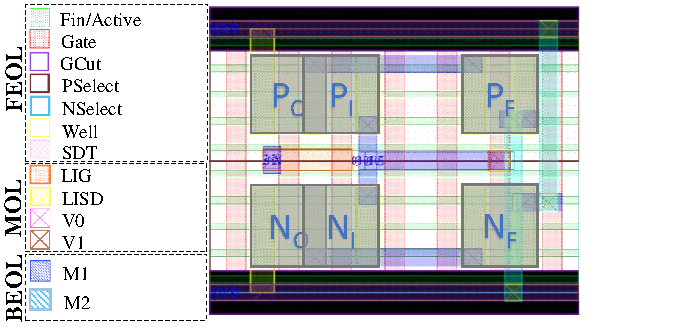
\includegraphics[width=0.85\textwidth, trim={0 0 1.5cm 0},clip]{camadasSTv2.pdf}
\caption{Technology layers and 3-fins transistors 6T ST layout}
\label{fig:layers}
\legend{Source: From the author.}
\end{figure}

\begin{table}[]
\centering
\caption{Each layout proportion/maximum number of fins, dimension and area (the TAP-Cell area is not taken into account).}
\label{tab:areas}
\resizebox{0.7\textwidth}{!}{%
\begin{tabular}{|c|c|c|c|c|}
\hline
                      & Layout & Height (nm) & Width (nm) & Area (nm²) \\ \hline
\multirow{5}{*}{INV}  & 1 Fin             & 270         & 162        & 43,740  \\ \cline{2-5}
                      & 2 Fins             & 270         & 162        & 43,740  \\ \cline{2-5}
                      & 3 Fins             & 270         & 162        & 43,740  \\ \cline{2-5}
                      & 4 Fins             & 324         & 162        & 52,488 \\ \cline{2-5}
                      & 5 Fins             & 378         & 162        & 61,236 \\ \hline
\multirow{5}{*}{ST}   & 1 Fin             & 270         & 378        & 102,060 \\ \cline{2-5}
                      & 2 Fins             & 270         & 378        & 102,060 \\ \cline{2-5}
                      & 3 Fins             & 270         & 378        & 102,060 \\ \cline{2-5}
                      & 4 Fins             & 324         & 378        & 122,472 \\ \cline{2-5}
                      & 5 Fins             & 378         & 378        & 142,884 \\ \hline
\multirow{5}{*}{SIG}  & 1 Fin             & 270         & 378        & 102,060 \\ \cline{2-5}
                      & 2 Fins             & 270         & 378        & 102,060 \\ \cline{2-5}
                      & 3 Fins             & 270         & 378        & 102,060 \\ \cline{2-5}
                      & 4 Fins             & 324         & 378        & 122,472 \\ \cline{2-5}
                      & 5 Fins             & 378         & 378        & 142,884 \\ \hline
\multirow{5}{*}{TIST} & 2 Fins : 1 Fin             & 270         & 270        & 72,900 \\ \cline{2-5}
                      & 4 Fins : 2 Fins             & 324         & 270        & 87,480  \\ \cline{2-5}
                      & 6 Fins : 3 Fins             & 432         & 270        & 116,640  \\ \cline{2-5}
                      & 3 Fins : 1 Fin             & 270         & 270        & 72,900 \\ \cline{2-5}
                      & 6 Fins : 2 Fins             & 432         & 270        & 116,640  \\ \hline
\end{tabular}%
}
\legend{Source: from the author.}
\end{table}

\begin{figure}[]
\centering
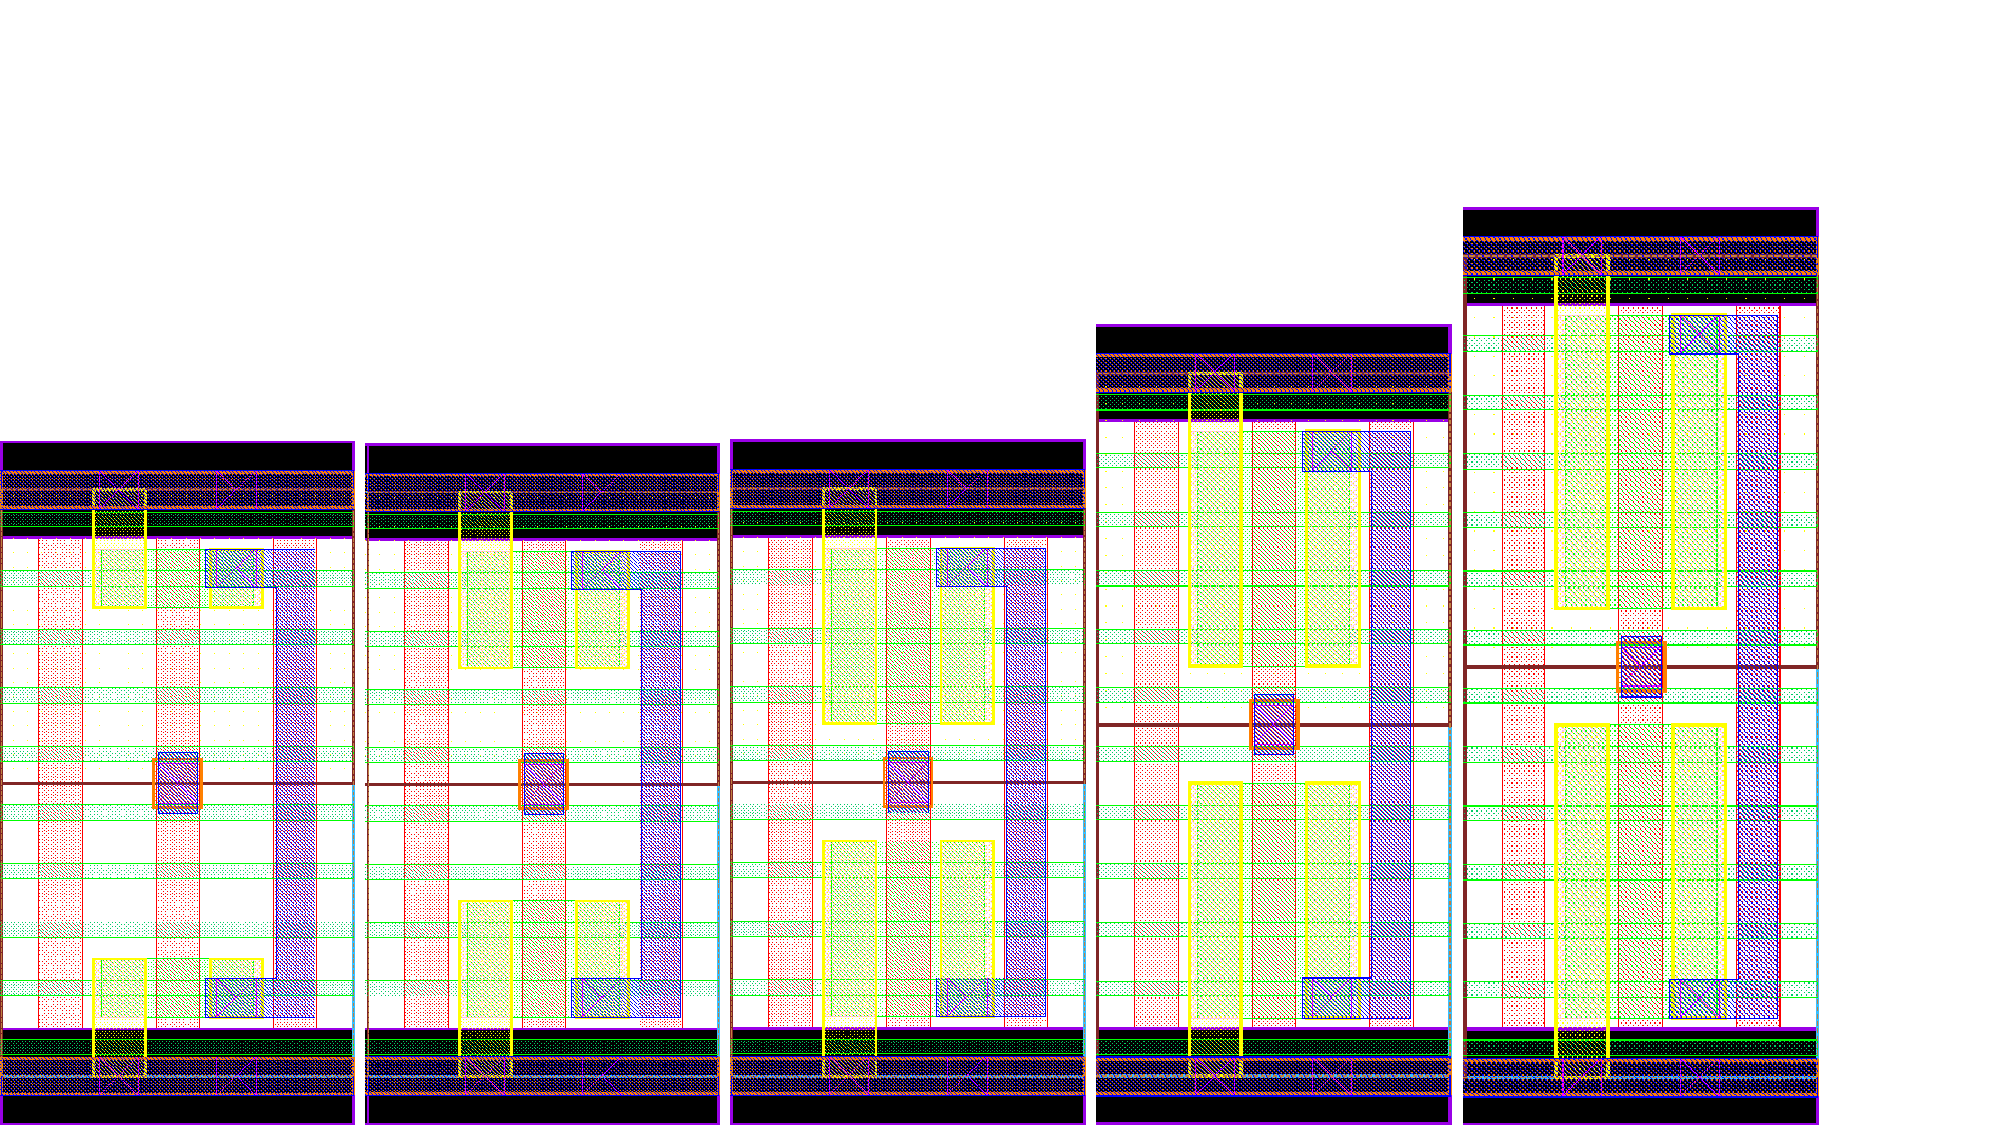
\includegraphics[width=0.425\textwidth, trim={0cm 0cm 4cm 3cm},clip]{INVComp.pdf}
\caption{1 to 5 fins (left to the right) traditional CMOS inverter layout comparison.}
\label{fig:invComp}
\legend{Source: From the author.}
\end{figure}

\begin{figure}[]
\centering
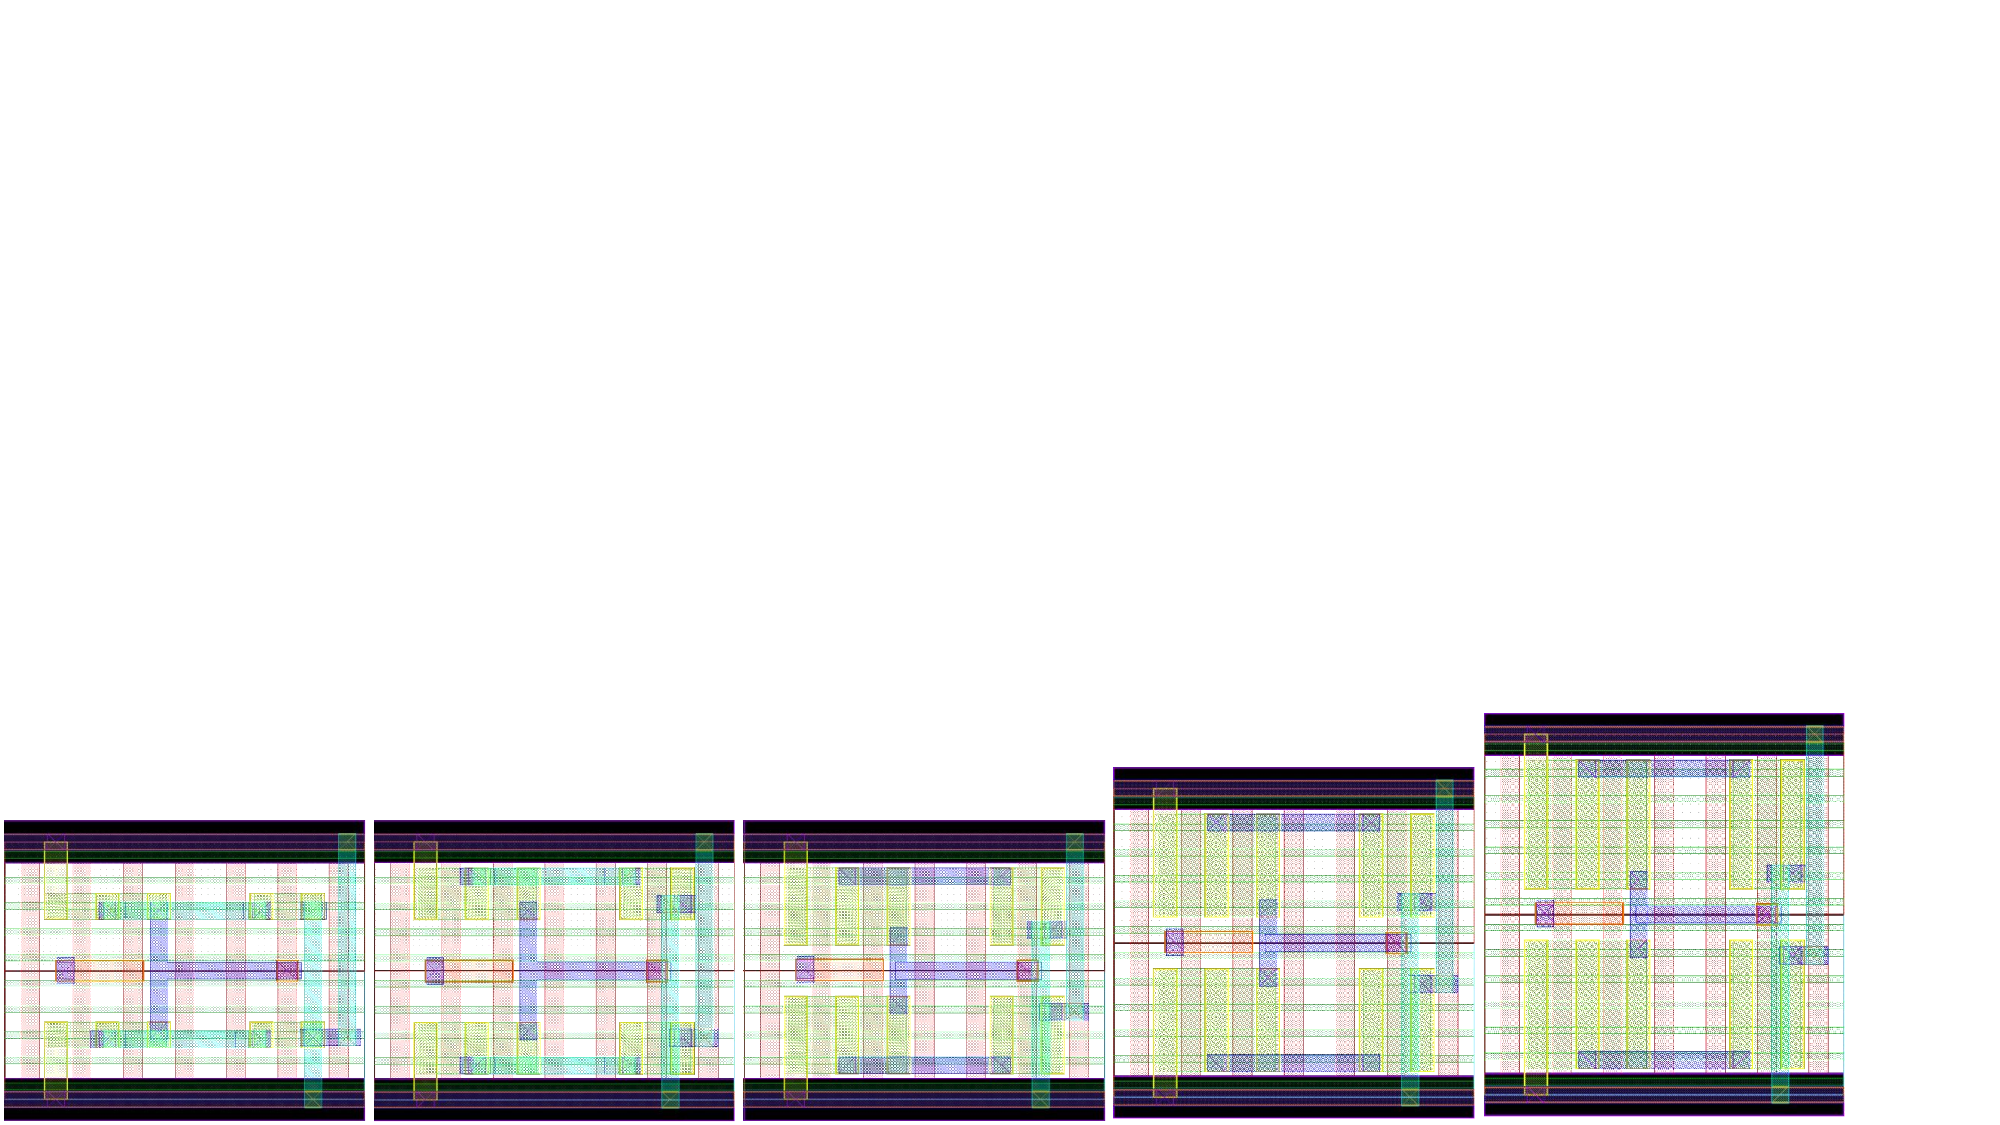
\includegraphics[width=\textwidth, trim={0cm 0cm 3cm 12cm},clip]{STComp.pdf}
\caption{1 to 5 fins (left to the right) ST layout comparison.}
\label{fig:stComp}
\legend{Source: From the author.}
\end{figure}

\begin{figure}[t]
\centering
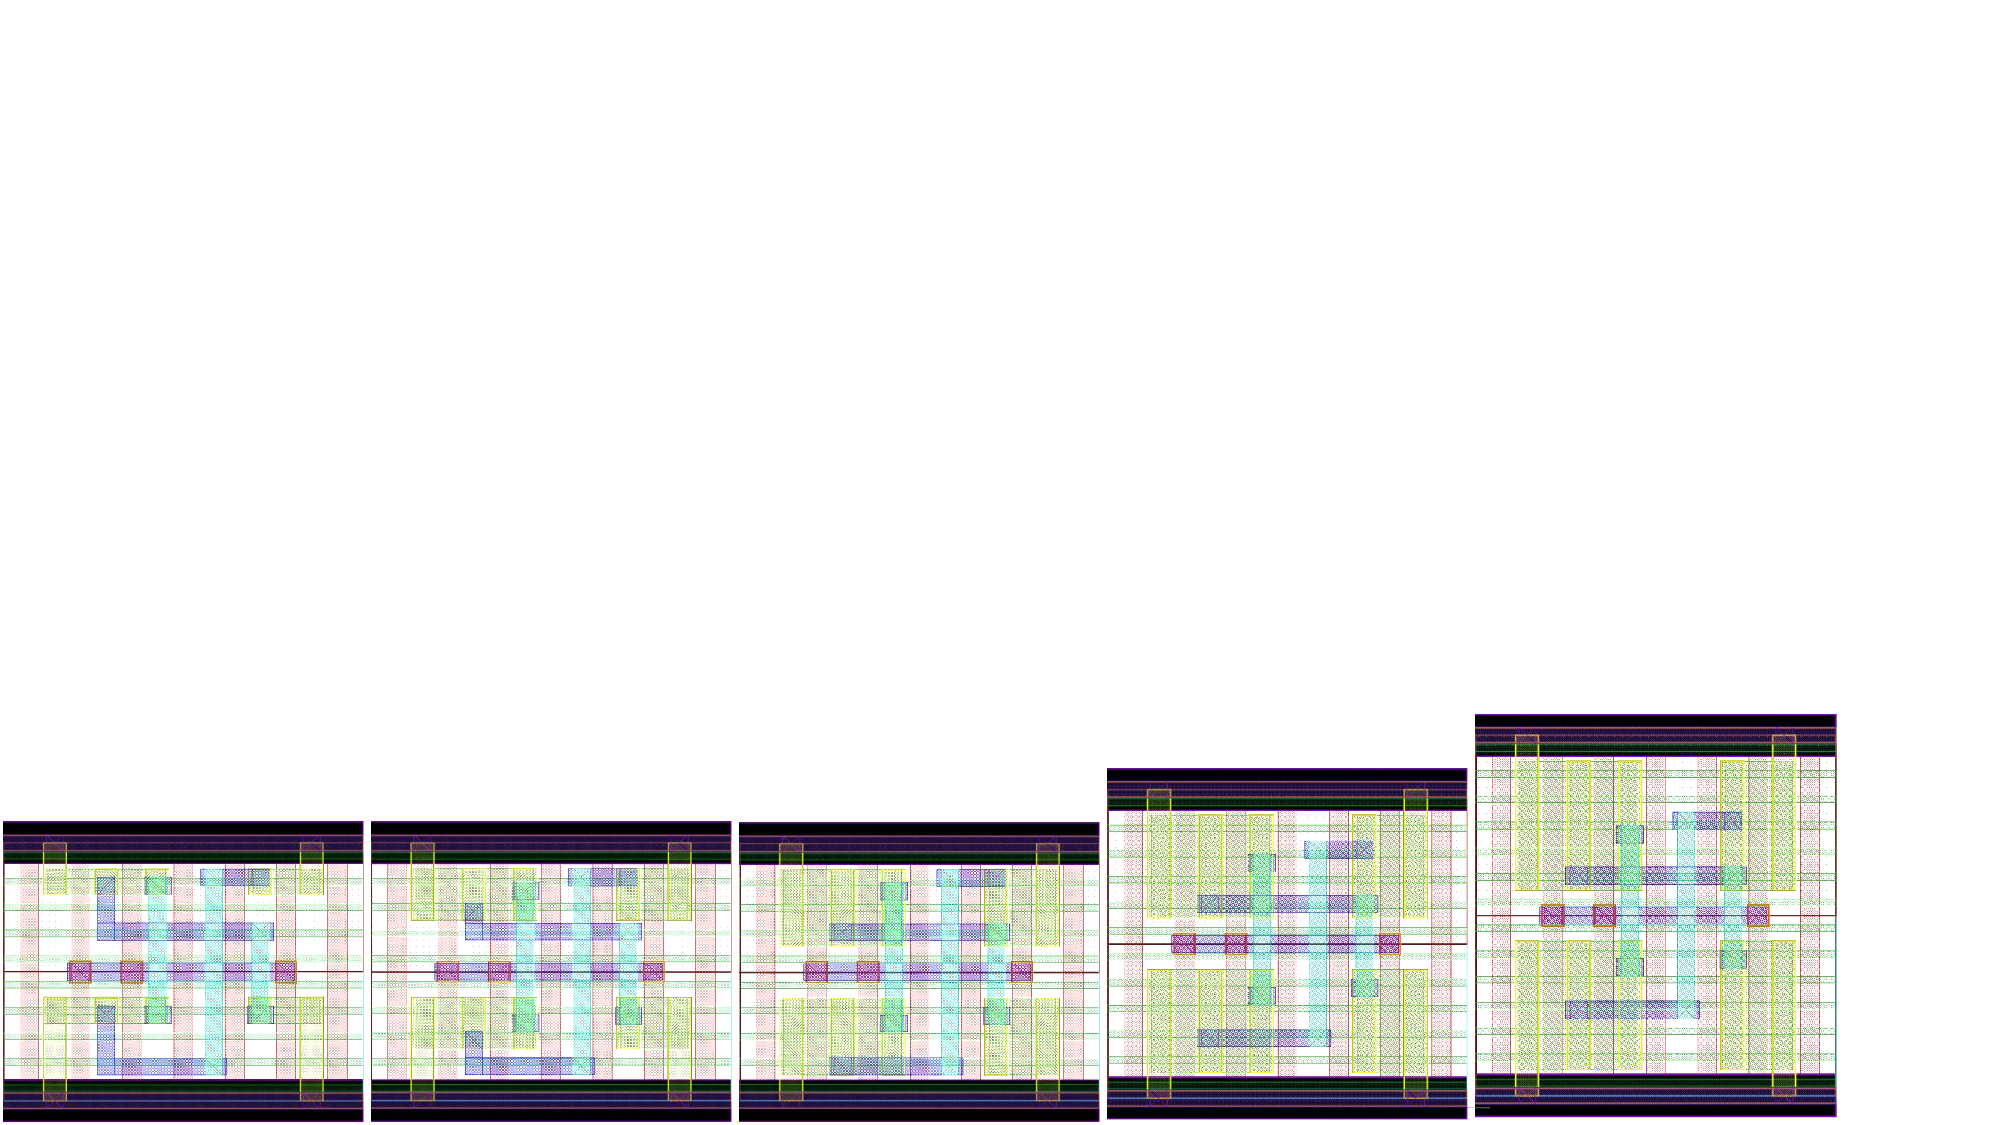
\includegraphics[width=\textwidth, trim={0cm 0cm 3cm 12cm},clip]{SIGComp.pdf}
\caption{1 to 5 fins (left to the right) SIG layout comparison.}
\label{fig:sigComp}
\legend{Source: From the author.}
\end{figure}

\begin{figure}[t]
\centering
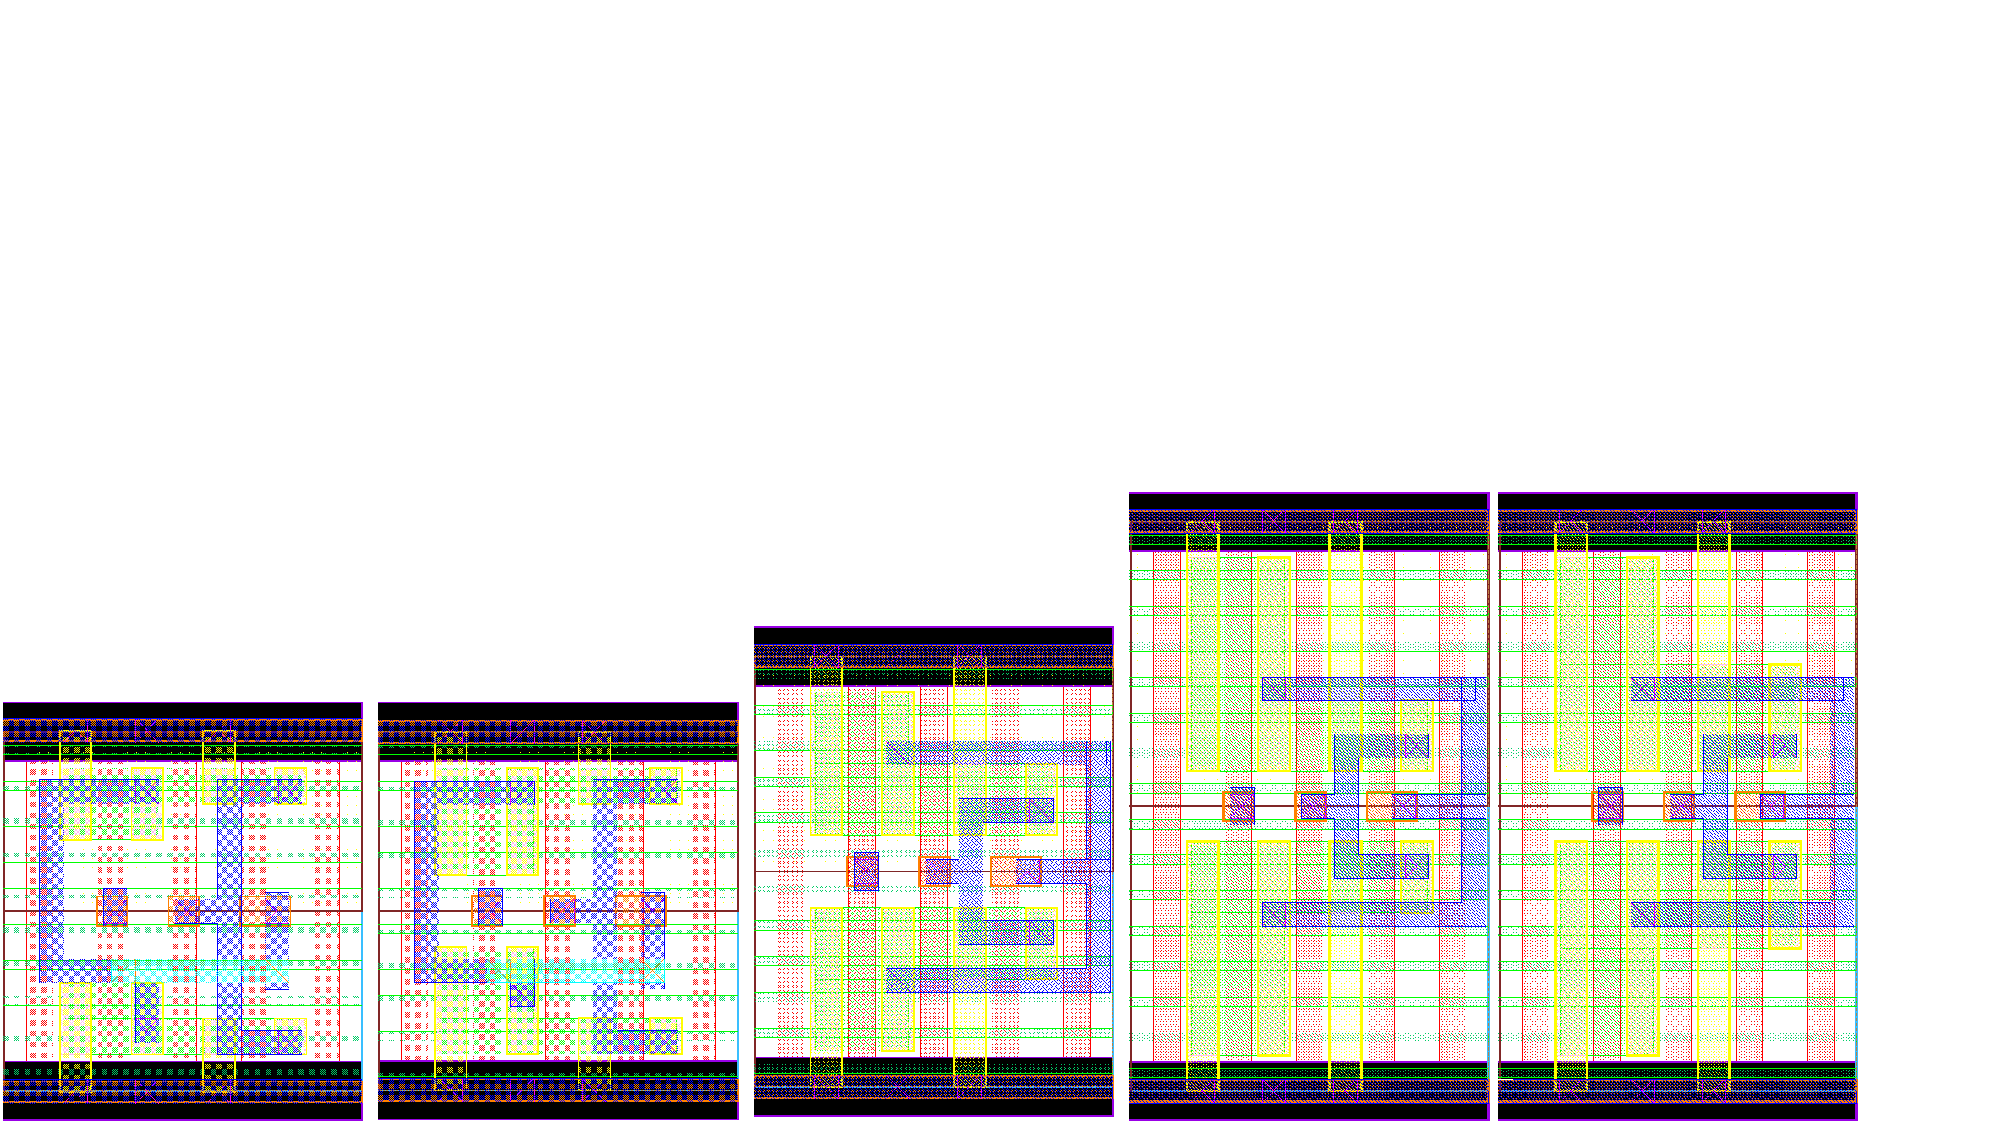
\includegraphics[width=0.65\textwidth, trim={0cm 0cm 3cm 8cm},clip]{TISTComp.pdf}
\caption{From the left to the right, 2, 4 and 6 maximum fins TIST layout comparison.}
\label{fig:tistComp}
\legend{Source: From the author.}
\end{figure}

\begin{table}[]
\centering
\caption{Key layer lithography assumptions, widths and pitches}
\label{layers}
\begin{tabular}{lccc}
\hline
\multicolumn{1}{c}{\textbf{Layer}} & \textbf{Lithography} & \textbf{Width/drawn (nm)} & \textbf{Pitch (nm)} \\ \hline
\textbf{Fin}                         & SAQP                 & 6.5/7                     & 27                  \\ \hline
\textbf{Active (horizontal)}         & EUV                  & 54/16                     & 108                 \\ \hline
\textbf{Gate}                        & SADP                 & 21/20                     & 54                  \\ \hline
\textbf{SDT/LISD}                    & EUV                  & 25/24                     & 54                  \\ \hline
\textbf{LIG}                         & EUV                  & 16/16                     & 54                  \\ \hline
\textbf{VIA0-VIA3}                   & EUV                  & 18/18                     & 25                  \\ \hline
\textbf{M1-M3}                       & EUV                  & 18/18                     & 36                  \\ \hline
\end{tabular}
\legend{Source: \citet{clark2016asap7}}
\end{table}

%\begin{figure}[]
%\centering
%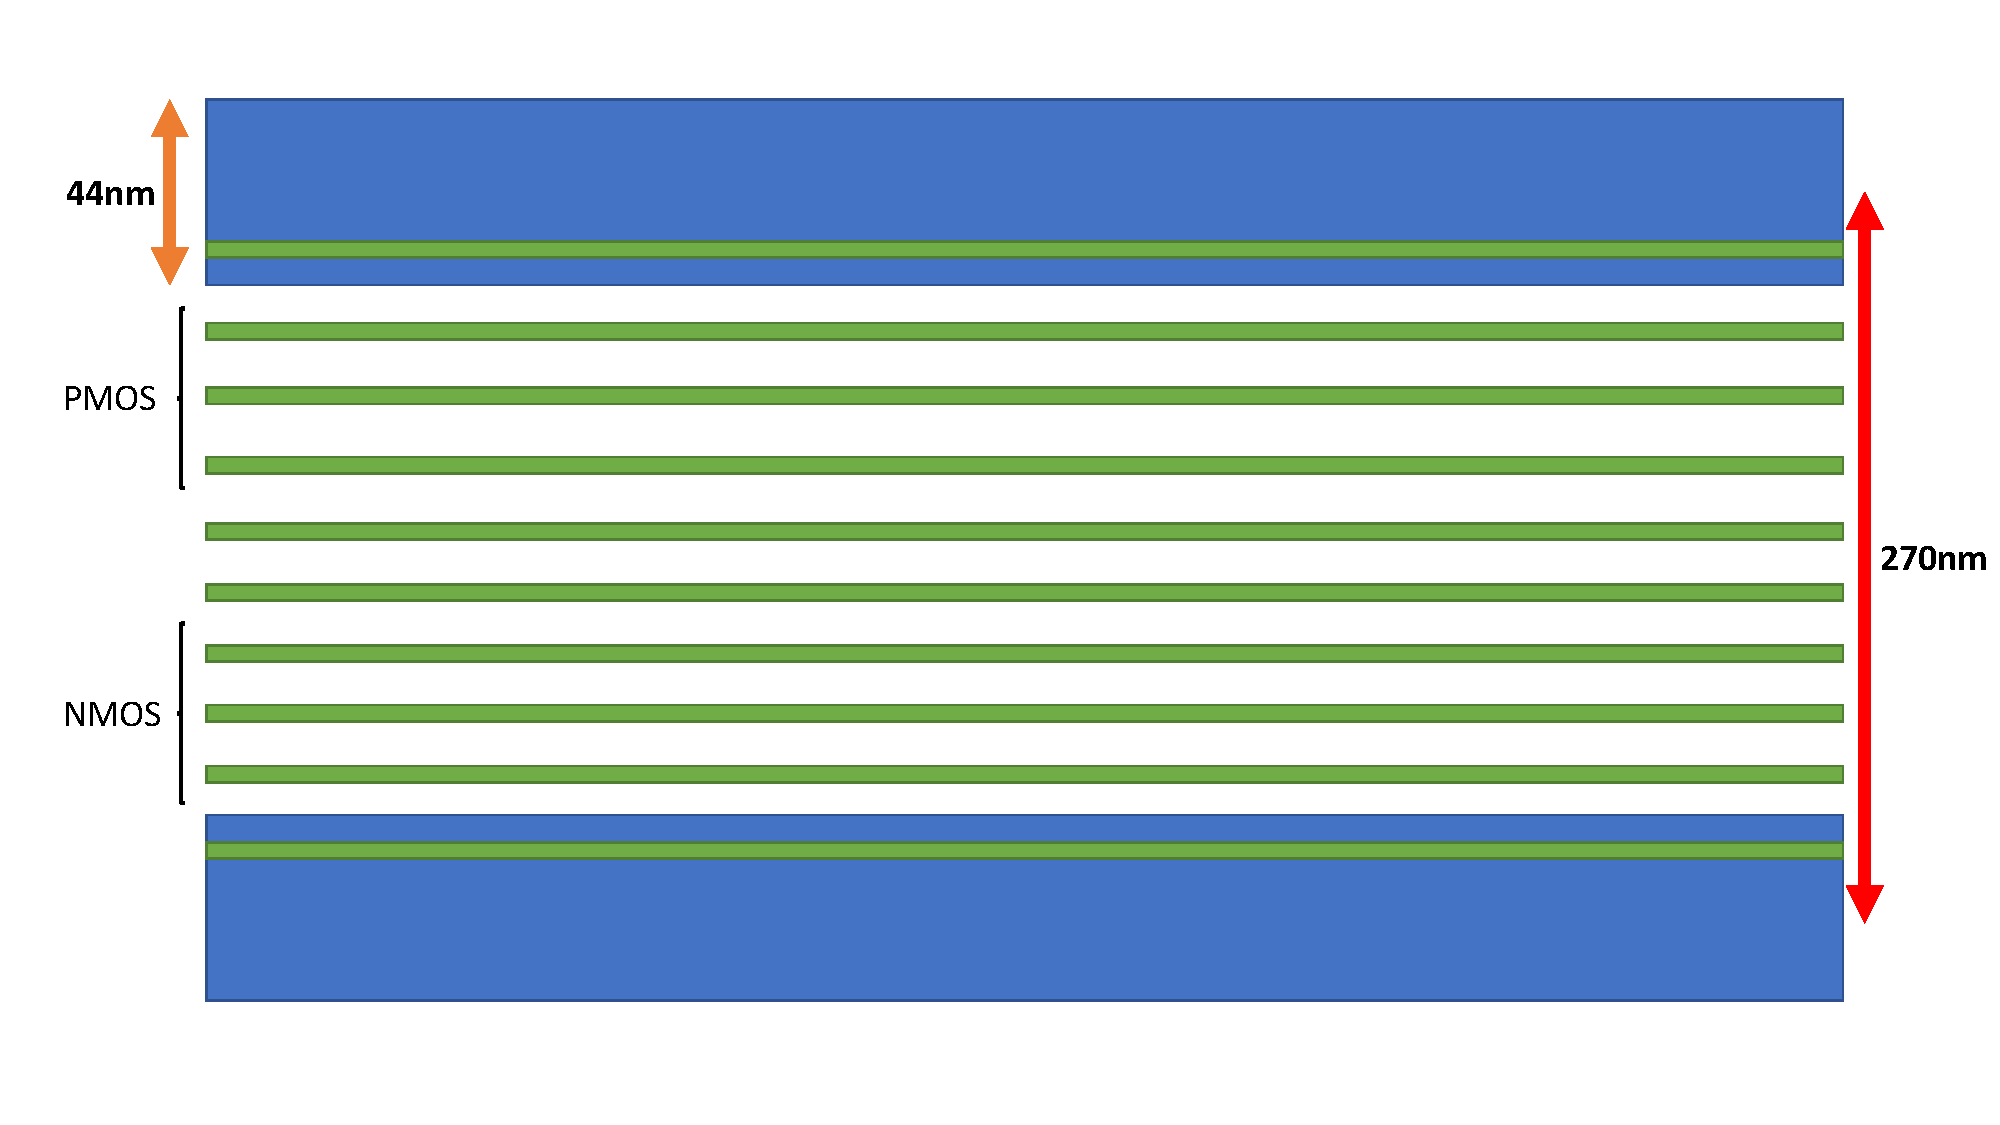
\includegraphics[width=0.8\textwidth]{transistorHeight.pdf}
%\caption{Transistor height and number of fins.}
%\label{th}
%\legend{Source: From the author.}
%\end{figure}


Due to technology restriction it is not possible to decrease the cell height when considering layout with a fin count below 3. In the case of the ST, for the layouts with a fin count below 3, M2 was applied to connect the source/drain of the ${P_F}$ and ${N_F}$ transistors to the X and Y layout nodes. For the TIST, for the layouts with less than 3 fins, M2 was necessary to connect the output signal to the $P_2$ and $N_2$ transistors gate. Given the smaller area to work with, it was necessary to apply M2 in order to respect the M1 spacing rules, bringing to light one of the challenges related to a smaller layout. The M2 usage in those cases will increase the design parasitics from the necessary extra vias connecting M1 and M2.


The ASAP7 PDK contains the manufacturing process composed by front end of line (FEOL), middle of line (MOL) and back end of line (BEOL). The layouts were developed in a continuous diffusion layer with every gate surrounding another gate in the horizontal axis. The Source-Drain Trench (SDT) connects the active area to the LISD layer. The Local-Interconnect Gate (LIG) is applied to connect the gate terminal, and Local-Interconnect Source-Drain (LISD) is used to connect the source and drain of the transistors. The function of Via 0 (V0) is to join the LIG and LISD to the BEOL layers. The Metal 1 (M1) is used for intra-cell routing and short connections. The Metal 2 (M2) was applied to connect the PF and NF drains to ground and source, respectively. To make the back-gate connections it is necessary a TAP-Cell. It is responsible to connect the NMOS and PMOS back-gates to supply/ground, respectively, being possible to connect the PMOS back-gates to another node. It is a PDK restriction needed for the proper function of the circuit. Its layout has a length of 108nm resulting in an area of 0.02916${\mu}m^{2}$ the 3-fins variant is shown in Figure \ref{tap}. In order to build the back-gate connections present in the LPST, it was necessary the insertion of TAP-Cells, greatly increasing the layouts size.

Furthermore, given the shared well of the NMOS devices, it was not possible to connect each NMOS back-gate to a specific node. Given so, the LPST NMOS transistors back-gates were connected to the ground, as shown in Fig \ref{fig:test}.

\section{Electrical Simulation}

The simulations will be carried out in HSPICE \footnote{https://www.synopsys.com/} using the netlist obtained after the physical verification flow and the parasitic capacitances extraction. The deviation on the device geometry impacts the electrical parameter WF causing high fluctuations \cite{zimpeck2016finfet}. It happens due to the orientation of metal grains randomly aligned in FinFET manufacturing process. In this way, WFF represents the most significant variation beyond the other parameters \cite{meinhardt2014impact}. The process variability evaluation will be taken through 2000 Monte Carlo (MC) simulations \cite{alioto2015variations} varying the WF of devices according to a Gaussian distribution considering a 3\(\sigma\) deviation. The reference values from ASAP7 technology for electrical simulations are shown in Table \ref{electPar}.

\begin{table}[]
\centering
\caption{Parameters applied in the electrical simulations}
\label{electPar}
\resizebox{0.5\textwidth}{!}{%
\begin{tabular}{lcc}
\hline
\textbf{Parameter}                                            & \multicolumn{2}{c}{\textbf{7nm}}                                  \\ \hline
\textbf{Nominal Supply Voltage}                               & \multicolumn{2}{c}{0.7 V}                                         \\ \hline
\textbf{Gate Length (L\textsc{g})}           & \multicolumn{2}{c}{21nm}                                          \\ \hline
\textbf{Fin Width (W\textsc{fin})}              & \multicolumn{2}{c}{6.5nm}                                         \\ \hline
\textbf{Fin Height (H\textsc{fin})}          & \multicolumn{2}{c}{32nm}                                          \\ \hline
\textbf{Oxide Thickness (T\textsc{ox})}      & \multicolumn{2}{c}{2.1nm}                                         \\ \hline
\textbf{Channel Doping}                                       & \multicolumn{2}{c}{$1x10^{22}m^{-3}$}                                     \\ \hline
\textbf{Source/Drain Doping}                                  & \multicolumn{2}{c}{$2x10^{22}m^{-3}$} \\ \hline
\multicolumn{1}{c}{\multirow{2}{*}{\textbf{Work Function (eV)}}} & NFET                            & 4.372                            \\ \cline{2-3}
\multicolumn{1}{c}{}                                        & PFET                            & 4.8108                           \\ \hline
\end{tabular}%
}
\legend{Source: \citet{clark2016asap7}}
\end{table}

\subsection{Inverters evaluation}
The WFF level for all simulations will range from 1\% to 5\% in 1\% steps on nominal values \cite{nawaz2014comparison}. For each step on WF variation, all simulations will be carried from 0.1V to 0.7V supply voltage, with 0.1V steps. For all experiments, it will be observed mean (\(\mu\)), standard deviation (\(\sigma\)) and normalized standard deviation (\(\sigma\)/\(\mu\)) for each metric: hysteresis interval, propagation times, energy, and on and off currents. The \(\sigma\)/\(\mu\) represents the sensibility of the cell to process variability, where the lower it is, highest is the robustness of the circuit to the impact of process variability.

The energy was calculated by integrating the current through time and multiplying by the supply voltage, and the propagation times where calculated by the timing difference between input and output signals to reach 50\% of its value ($V_{DD}/2$). Additionally, noise margins, gains and VTC curve slopes will be presented. The noise margins were calculated as shown in Fig. \ref{fig:SNM} where the margin values are extracted from the VTC curve points where the derivative/slope is -1. The slopes were calculated following the equation \ref{eqn:slope}, based on Fig. \ref{fig:SNM}.

For the maximum frequencies, each time there was 10\% or more of failed simulations, from the 2000 MC, the frequency was decreased. On the contrary, if there was less than 10\% of failures, the frequency was increased. At each increase/decrease the simulations were performed again. The minimum frequency considered for the circuit to be considered functional at determined sizing, supply voltage, and level of variability is 50KHz. This frequency was chosen in order to save resources and bring a wide frequency range.


\begin{figure}[]
\centering
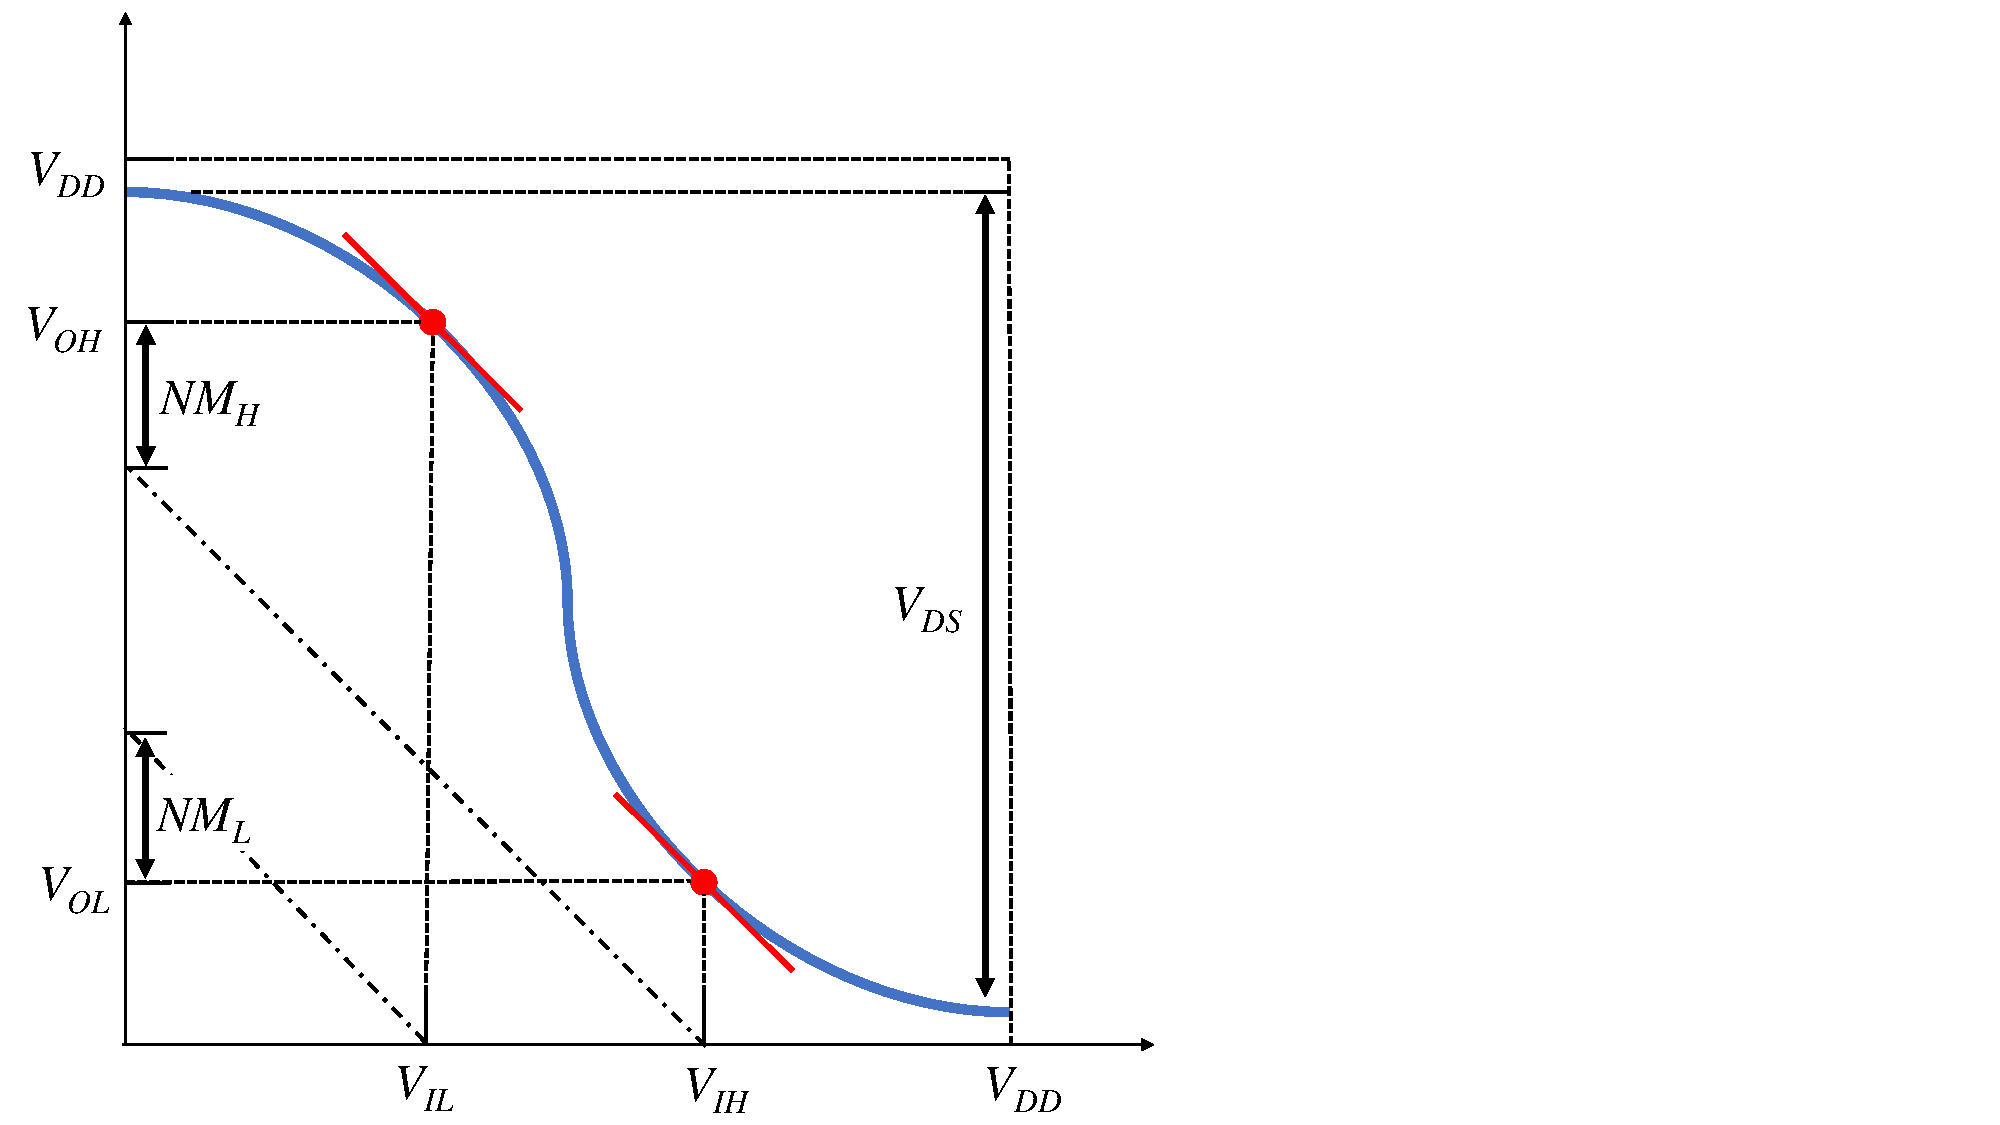
\includegraphics[width=0.6\textwidth, trim={0cm 0cm 14cm 0cm},clip]{SNM.pdf}
\caption{Noise margins measurements.}
\label{fig:SNM}
\legend{Source: \citet{schrom1997vlsi}.}
\end{figure}

\begin{equation}
    \centering
    \label{eqn:slope}
    Slope = \frac{V_{OH} - V_{OL}}{V_{IH} - V_{IL}}
\end{equation}

 For a more realistic test-bench, it will be considered a scenario where the Device Under Test (DUT) receives the signal passing through two inverters in series and having a 1fF output capacitance, as shown in Fig. \ref{fig:tbST}. It is essential to consider some details such as: the same supply voltage is applied in the entire testbench, only the DUT suffers from variability, the inverters are the same (3-fins transistors) for all experiments, and they are, like the DUT, simulated from the extracted layout.

\begin{figure}[]
\centering
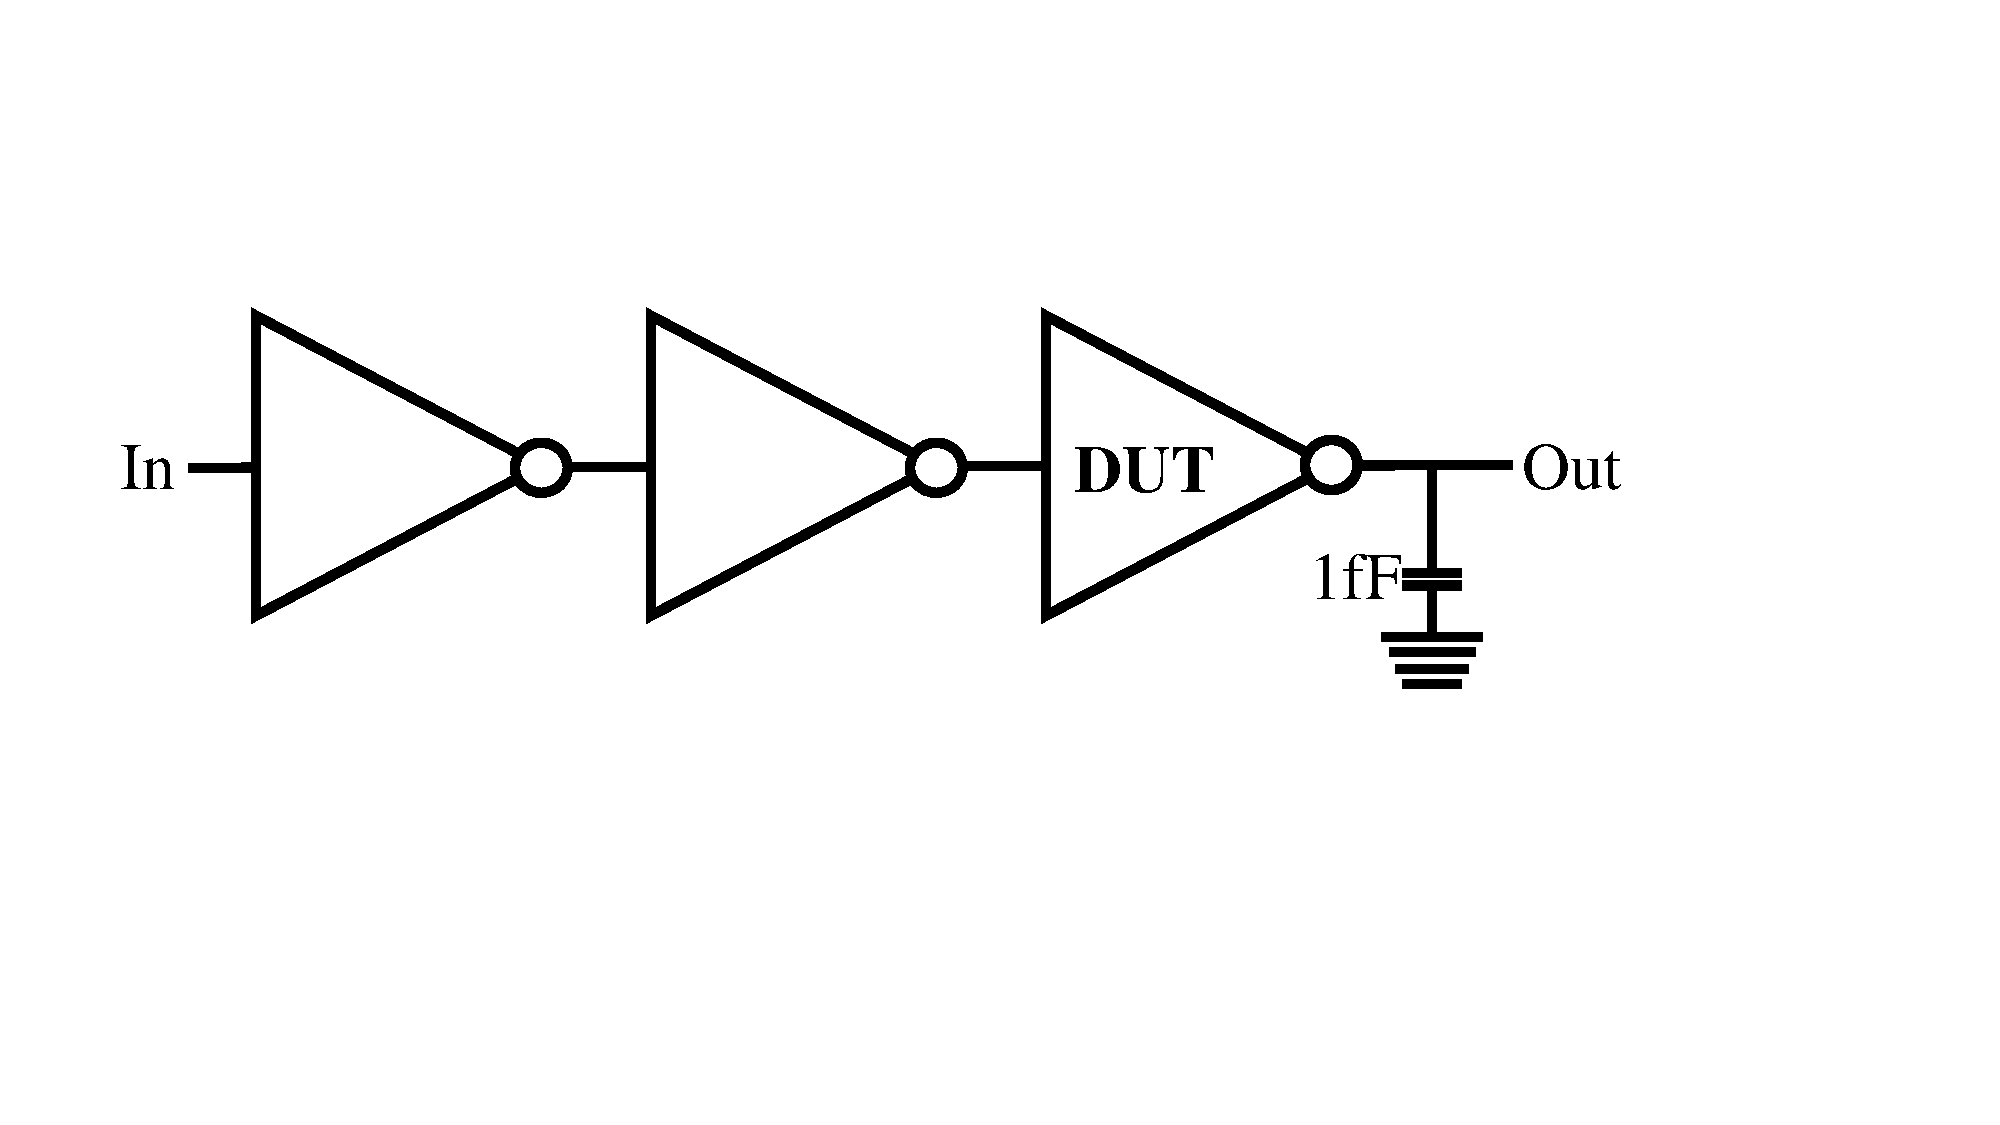
\includegraphics[width=0.6\textwidth, trim={2cm 7cm 6cm 5cm},clip]{testbench.pdf}
\caption{Test-bench.}
\label{fig:tbST}
\legend{Source: From the author.}
\end{figure}

\subsection{ST technique on Full Adders}

To provide an analysis of the impact of the replacement of FAs internal inverters with STs, it was considered four different types of Full Adders topologies to evaluate their robustness to process variability. In order to analyze such impact:

1) All FAs will be analyzed with the same sizing of 3 fins;

2) Each FA will have 3 versions: the traditional (internal inverters not replaced), the FA with its internal inverters replaced by LPST, and the FA with its internal inverters replaced by the 6TST.

3) It will be considered only one level of variability of 5\% WFF, following a Gaussian distribution.

4) There will be considered two level of supply voltage: nominal (0.7V) and near-threshold (0.4V).

The Full Adders listed below have been chosen due to their promising results in related and previous works \cite{ames2016investigating,dokania2015circuit,dokania2013investigation,moraes2018evaluation}:

\begin{enumerate}
    \item Complementary MOSFET Mirror  Adder (Mirror)
    \item Transmission Gate Adder (TGA)
    \item Transmission Function Adder (TFA)
    \item Hybrid Full Adder
\end{enumerate}

The Mirror Full Adder is considered the most traditional Full Adder topology containing 28 Transistors arranged in a pull-up and pull-down networks, which are logically complementary. It has a full voltage swing and buffered Sum and Cout signal and the advantages of good conductibility and robustness when working with novel technologies and low voltages. However, it has high capacitance because each input is connected to the gate of at least a p-channel metal-oxide-semiconductor (PMOS) and n-channel metal-oxide-semiconductor (NMOS) device additionally, it shows the impact of the pull-up network that makes the circuit slower due to the low mobility of its holes \cite{beckett2002fine} \cite{devadas2017design} \cite{islam2011design}.

Transmission Gate Full Adder \cite{weste1985principles} contains 16 transistors, and is a high speed and low power design. However, shows low driving capability which may be unacceptable in some cases where there is a long chain of full adders due to the increase in delay \cite{islam2011design}. The Transmission Function Adder is based on transmission gates as well, containing 20 transistors, working satisfactorily with low voltages but losing performance when cascaded due to the lack of supply/ground contacts and, consequently, driving capability \cite{navi2009novel}. Both TFA and TGA generate the XOR function (H = A XOR B) followed by an inverter which produces the XNOR function (H’). H and H’ are used to control the transmission gates generating the Sum and Cout outputs. The inverter generates delay between H and H’, which will cause the transmission gates to behave as pass transistors, that may introduce glitches and consequently, increase the power consumption of these cells. Additionally, TGA contains three inverters, one more than TFA. The inverters switching introduce more short-circuit power \cite{shams2000novel}.

Inspired by CMOS and CPL Full Adders architectures, the Hybrid Full Adder \cite{navi2009novel} contains 26 transistors, with the main advantage of a high output signal and low power properties. Although, the design shows high input capacitance for specific input vectors. The Full Adder designs are shown in Figure \ref{fig:FAs}.

\begin{figure}[]
\centering
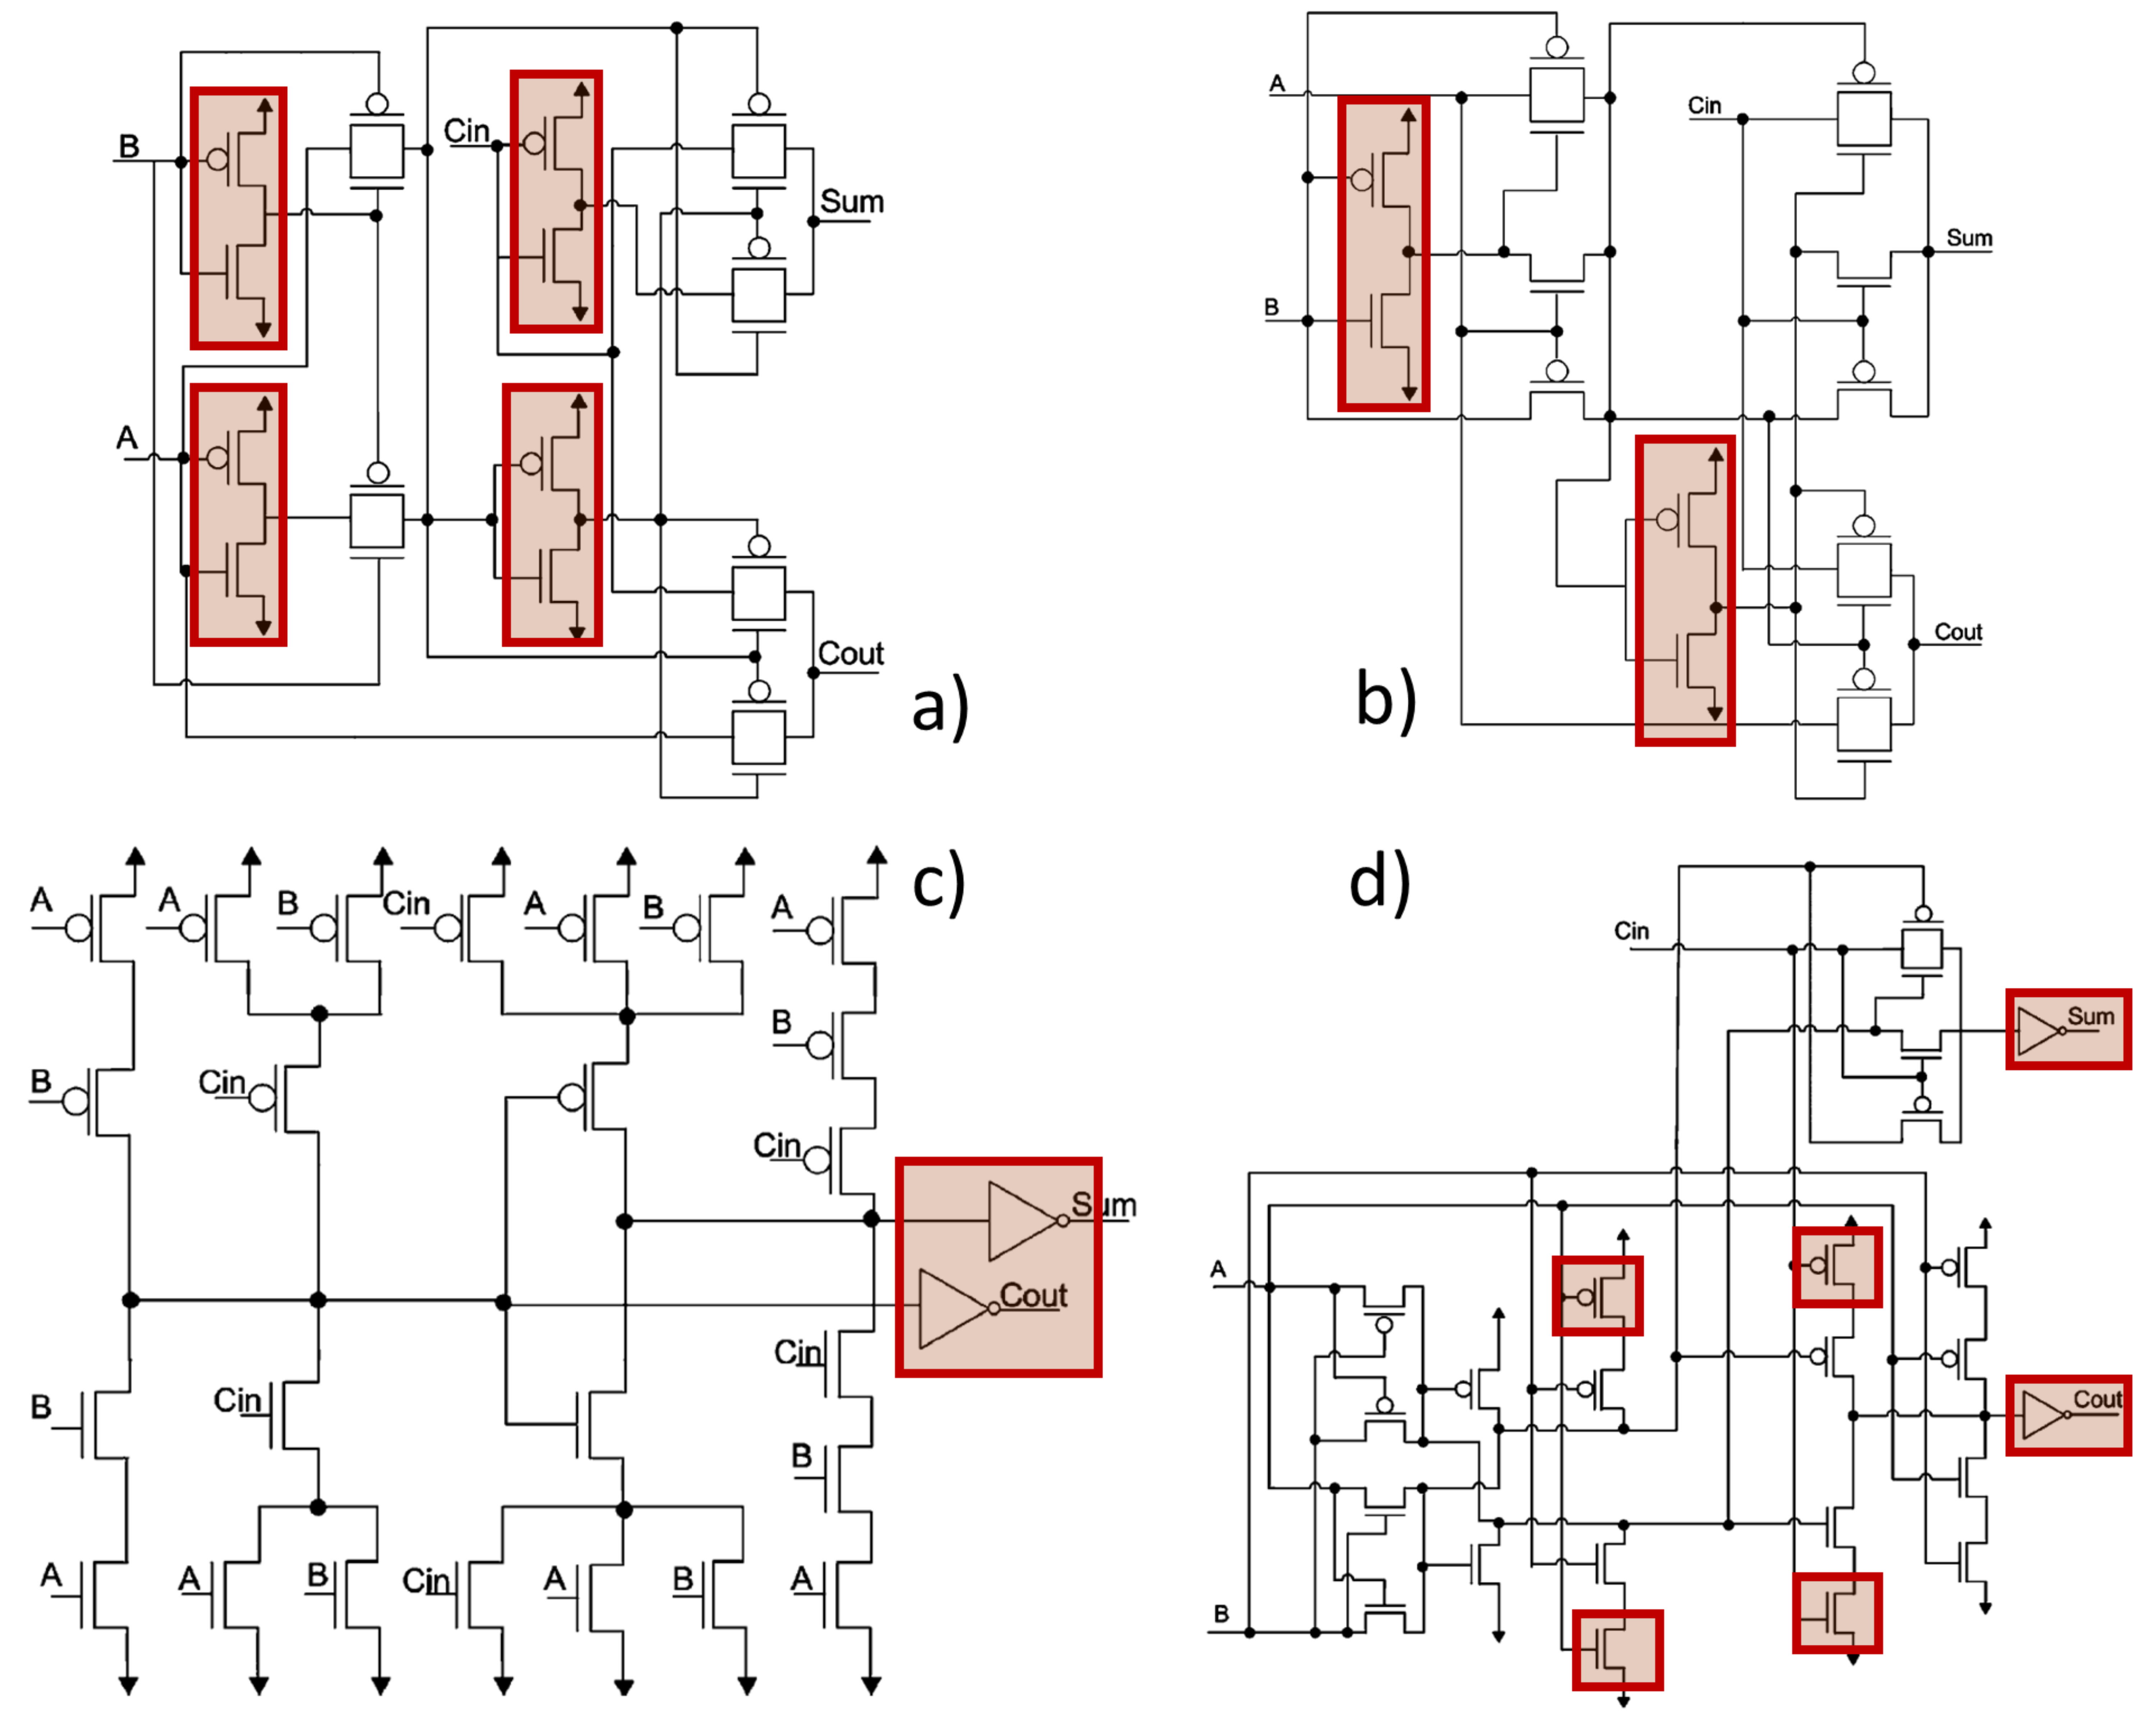
\includegraphics[width=1\textwidth]{FAs.png}
\caption{Full Adders with internal inverters to be replaced highlighted.}
\label{fig:FAs}
\legend{Transmission Gate Adder (a), Transmission Function Adder (b), Mirror CMOS Adder (c) and Hybrid Full Adder (d).
Source: \citet{samuel2016}}
\end{figure}


For the simulations concerning the Full Adders, it was considered two levels of supply voltage, near-threshold (0.4V) and nominal (0.7V) and single level of WFF level of 5\%. For the metrics, it was considered the mean, standard deviations, and normalized standard deviations for the energy and delay measures. The test-bench applied consists of a 5-bit Ripple Carrier Adder with with each output (Sum outputs for each FA and last Carry Out) connected to a fan-out of 4 inverters, as shown in Fig \ref{fig:tbFA}. In order to extract the delay and energy measures, an input vector was applied to trigger a pair of transitions (high-to-low and low-to-high) for each output (Sum and Carry Out) in relation to each input (A, B and C).

\begin{figure}[]
\centering
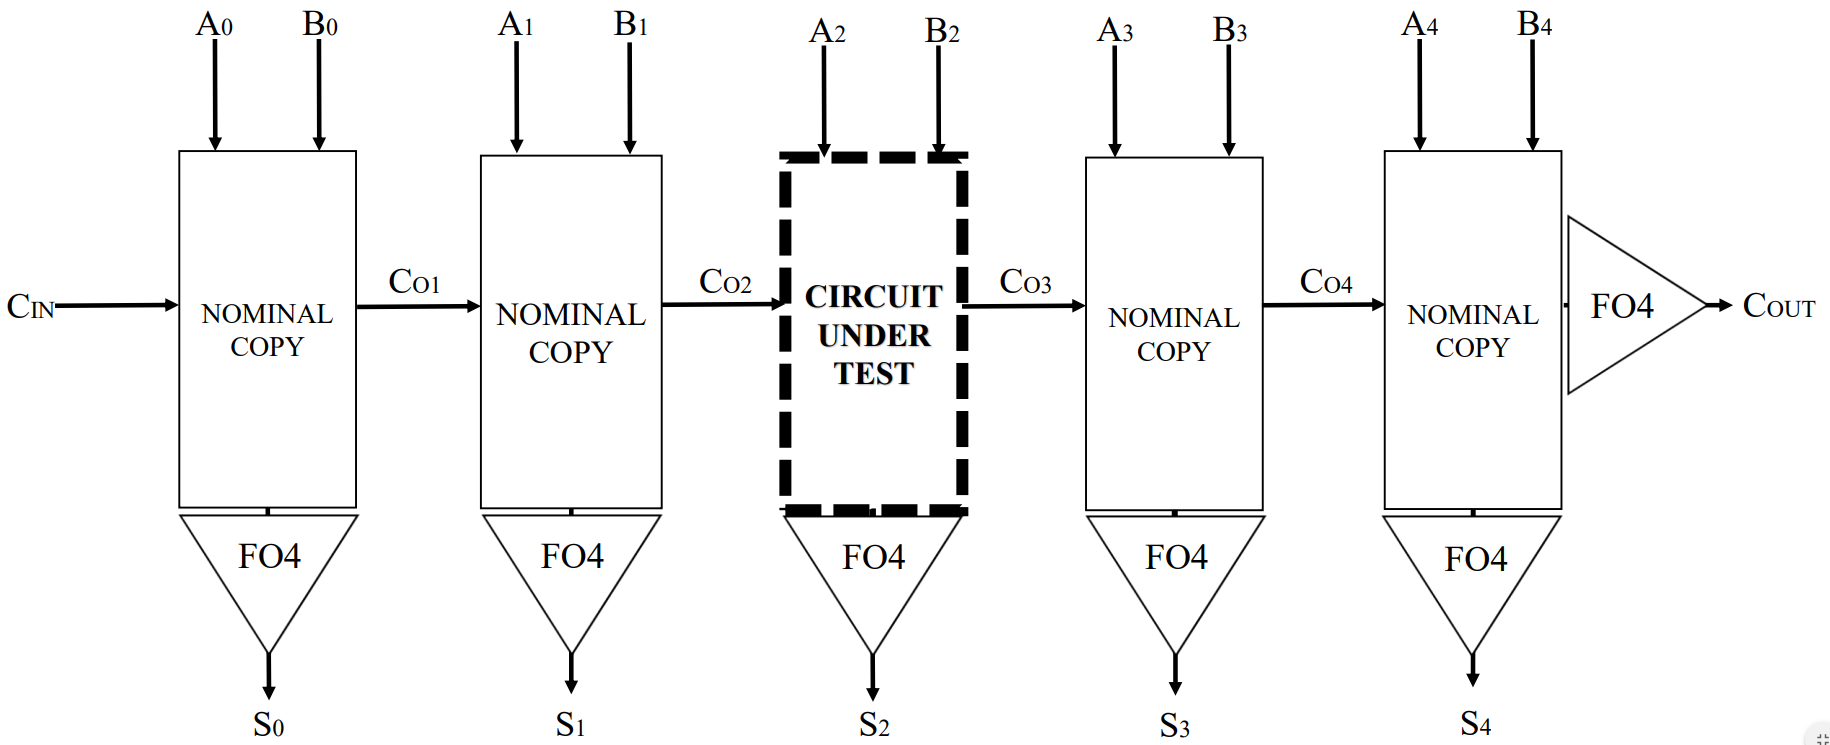
\includegraphics[width=\textwidth, trim={0cm 0cm 0cm 0cm},clip]{testbenchFA.png}
\caption{Test-bench for the Full Adders simulation.}
\label{fig:tbFA}
\legend{Source: From the author.}
\end{figure}

Each FA area is shown in Table \ref{tab:FAareas} where the LPST and traditional 6T ST are renamed as ST1 and ST2, respectively. All FAs layouts were designed with a dense 7.5 M2 (Metal 2) track cell, baseline resulting in a 270nm cell height. This corresponds to three fins for each transistor. All FA layouts are shown in Appendix B.

\begin{table}[]
\centering
\caption{Each Full Adder area with the ST technique applied where ST1 and ST2 corresponds to the LPST and 6T ST, respectively.}
\label{tab:FAareas}
\resizebox{0.7\textwidth}{!}{%
\begin{tabular}{|c|c|c|c|c|}
\hline
Full Adder & \# Transistors & Width (nm)  & Area (nm²) & Ratio \\ \hline
Mirror     & 28		   & 1,188       & 320,760    & -     \\ \hline
Mirror ST1 & 32            & 2,808       & 758,160    & 2.36  \\ \hline
Mirror ST2 & 36            & 1,836       & 495,720    & 1.55  \\ \hline
TGA        & 20            & 1,836       & 495,720    & -     \\ \hline
TGA ST1    & 28            & 5,292       & 1,428,840  & 2.88  \\ \hline
TGA ST2    & 36            & 2,916       & 787,320    & 1.59  \\ \hline
TFA        & 16            & 1,620       & 437,400     & -    \\ \hline
TFA ST1    & 20            & 3,240       & 874,800     & 2.00 \\ \hline
TFA ST2    & 24            & 2,052       & 554,040     & 1.27 \\ \hline
HYBRID     & 26            & 1,728       & 466,560     & -    \\ \hline
HYBRID ST1 & 34            & 5,292       & 1,428,840   & 3.06 \\ \hline
HYBRID ST2 & 42            & 2,916       & 787,320     & 1.69 \\ \hline
\end{tabular}%
}
\legend{Source: from the author.}
\end{table}

\begin{figure}[t]
\centering
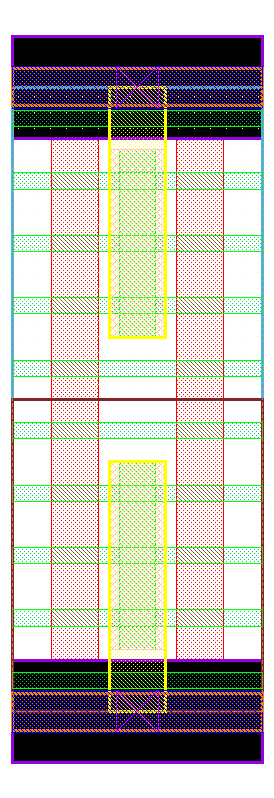
\includegraphics[width=0.2\textwidth]{TAP.png}
\caption{TAP-Cell Layout.}
\label{tap}
\legend{Source: From the author.}
\end{figure}

\begin{figure}[]
\centering
\begin{subfigure}{.5\textwidth}
  \centering
  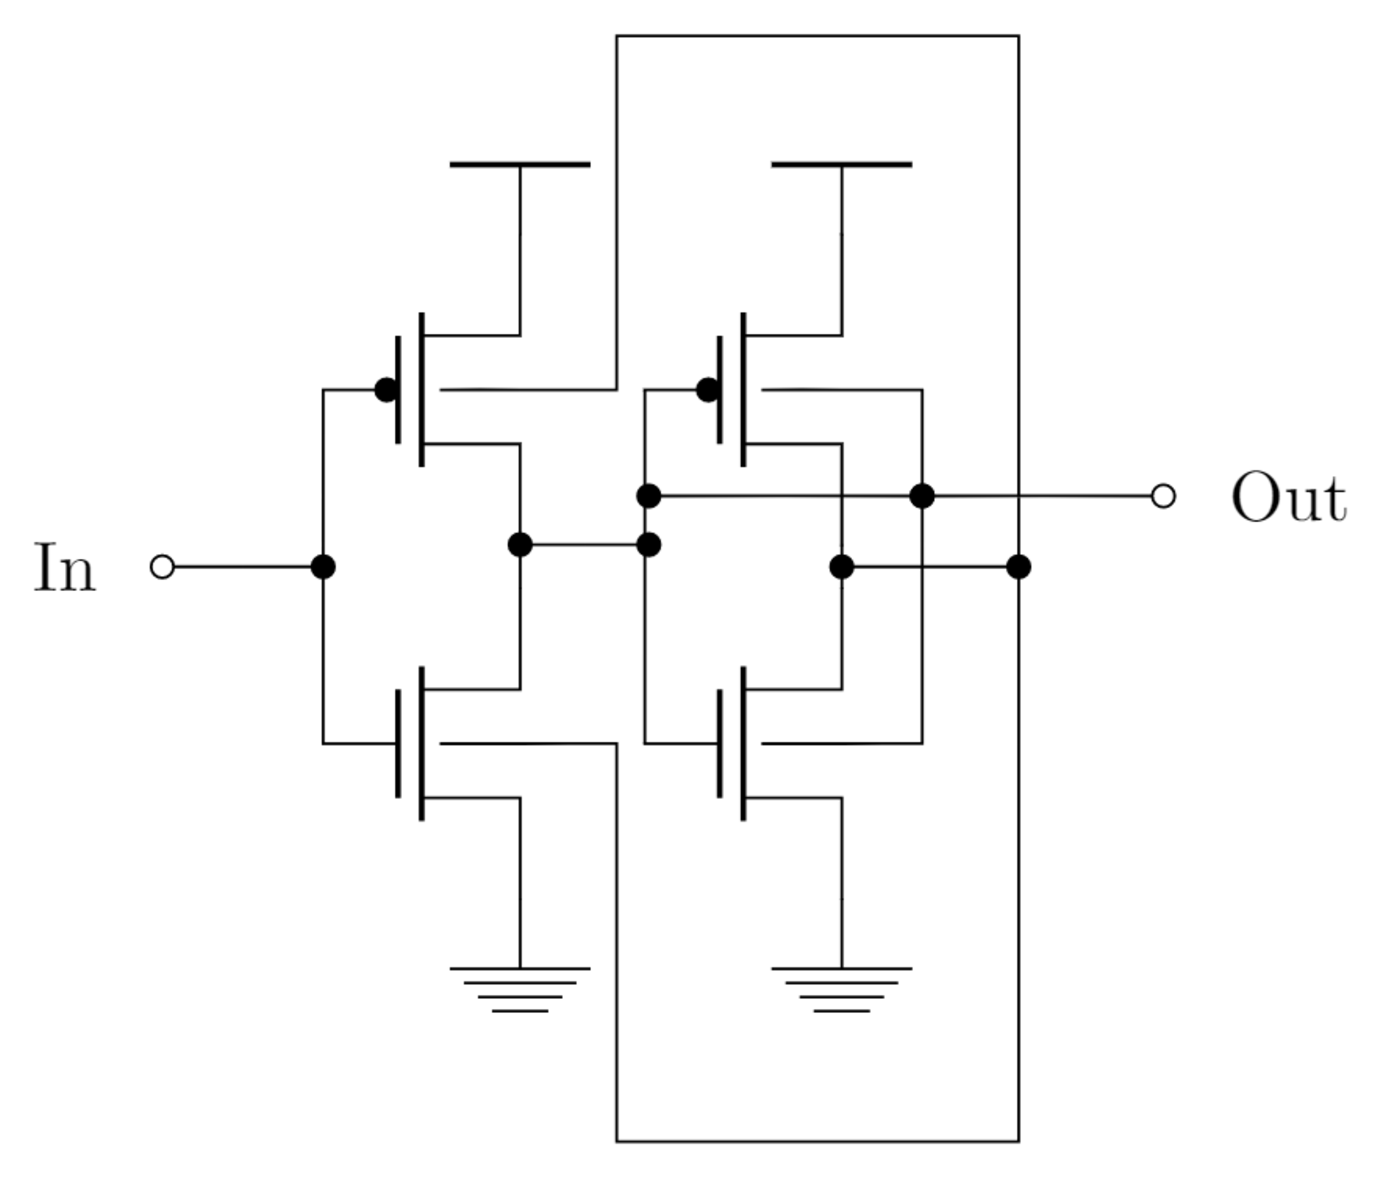
\includegraphics[width=.8\linewidth]{STOriginal.eps}
  \caption{LPST Inverter from \citet{dokania2015circuit}}
  \label{fig:sub1}
\end{subfigure}%
\begin{subfigure}{.5\textwidth}
  \centering
  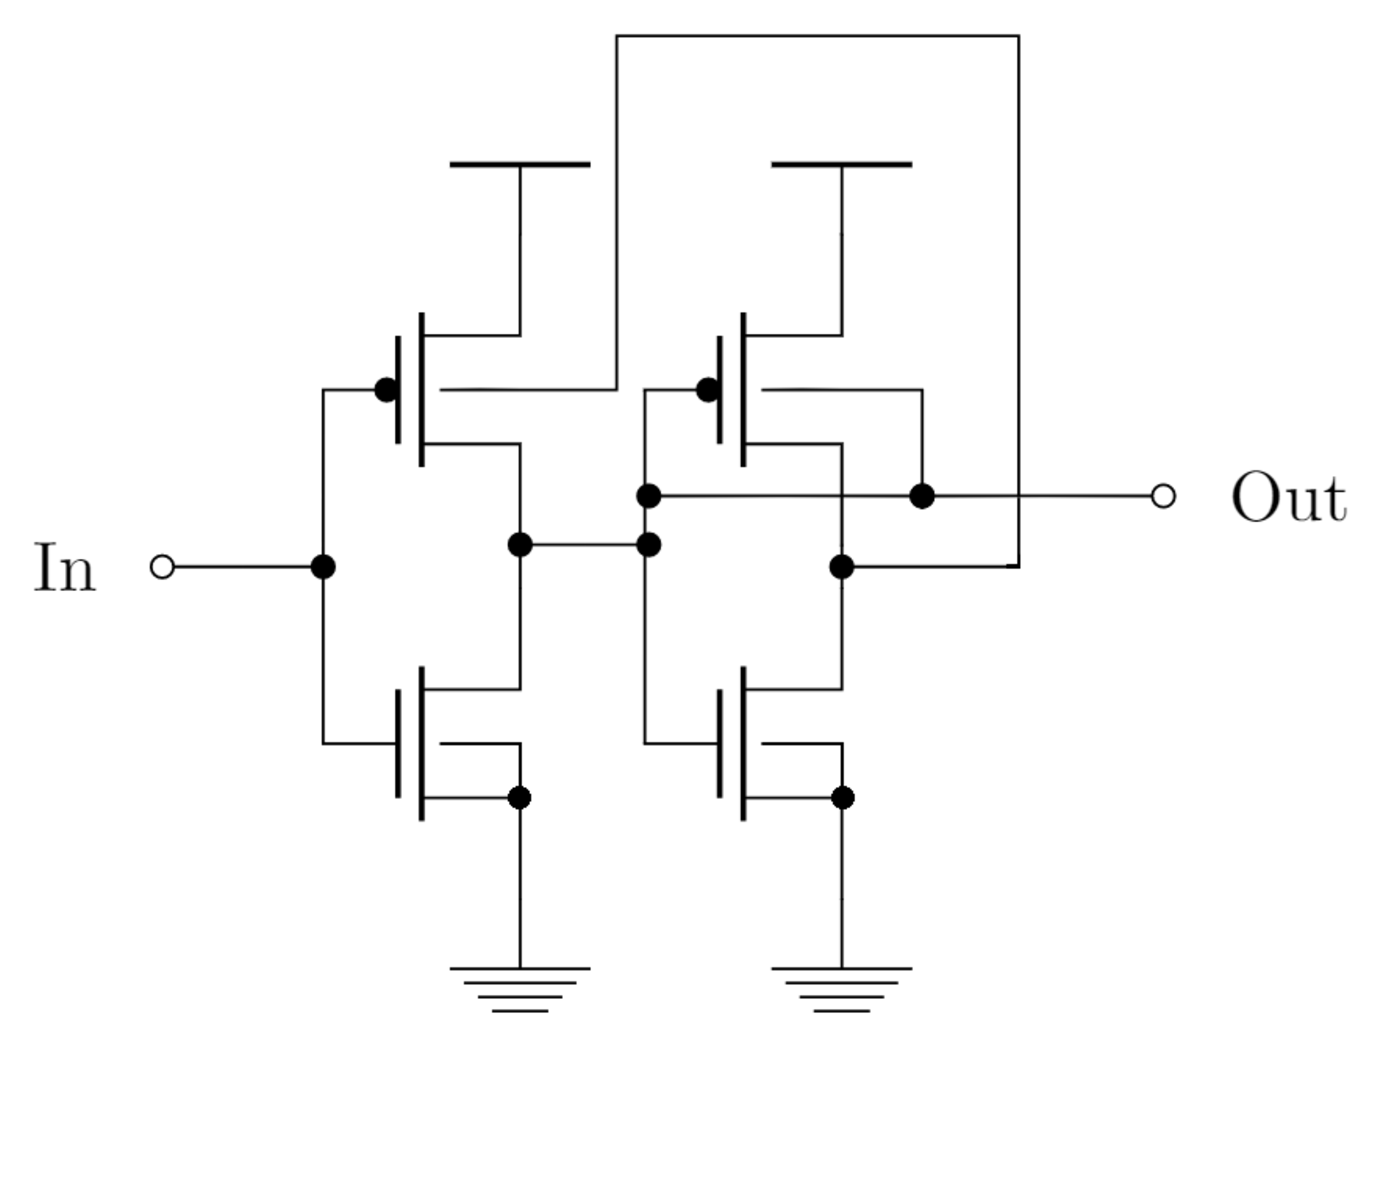
\includegraphics[width=.8\linewidth]{STcorrigido.eps}
  \caption{Modified LPST Inverter applied in this work. Source: From the author.}
  \label{fig:sub2}
\end{subfigure}
\caption{Original and modified Low Power STs (LPST) side-by-side}
\label{fig:test}
\end{figure}

% Please add the following required packages to your document preamble:
% \usepackage{multirow}

\chapter{Evaluation of ST Circuits and Alternatives}

The analysis of the behaviour of several inverter under the effects of process variability will be divided in sections concerning the metrics. The first section will be about the maximum frequency reached by each design depending on the supply voltage and the level of process variability and the scenarios, sets of supply voltage and level of variability, at which the frequency did not remain above 50KHz. The second section will lay out the propagation times, since the frequency already gives a good notion about the circuits performance, this section will show the propagation times deviations, presenting each design behavior.

The third section will lay the results concerning the energy consumption and deviation. The designs will be compared to one another and the impact between each supply voltage and number of fins will be considered. Additionally, considering different types of applications - minimum energy, highest robustness, and cost-benefit - different sets of supply voltages and transistor sizing will be recommended for each level of variability, where patterns are identified. The currents and current ratios will be discussed in the forth section, where measures and deviations will be shown, as well the increase scaling through the variability levels. Further on, SNM measures, output gains and slopes, hysteresis, and measures histograms will be discussed at the fifth, sixth, seventh, and eighth, respectively.

\section{Non-viable scenarios and Frequencies}

Across the simulations, as the variability level scaled and supply voltage decreased, in order to maintain the percentage of failures below 10\%, the circuits frequency had to be reducted. For the traditional inverter, ST, and SIG, the considered \textit{non-viable} scenarios (when the viable frequency of operation is below or at 50KHz) started to appear at 200mV, for any scenario above 4\% WFF, and 100mV for any scenario above 5\% WFF.

The TIST presented a particular behavior, with its hysteresis interval growing too large as supply voltages got higher. The TIST got the same subset of \textit{non-viable} scenarios of the previous designs, although due to its hysteresis, sub- to near-threshold supply voltages did not work apropriately.

The TIST 2:1 designs did not present any viable scenarios at 200mV and 300mV, with only low-variability scenarios (1\% and 2\% WFF) working at 0.4V and 0.5V. The TIST 3:1 designs presented a slight improvement with viable scenarios at 200mV and 300mV at 1\% WFF. For 0.4V and 0.5V the TIST 3:1 presented to be more viable, although not working at high to medium level of variability (3\%~5\% WFF). The frequencies for each scenarios are shown at Table \ref{tab:freqs}.

\begin{table}[t]
\centering
\caption{All scenarios frequencies.}
\label{tab:freqs}
\resizebox{\textwidth}{!}{
\begin{tabular}{|c|c|c|c|c|c|c|c|c|}
\hline
\multirow{2}{*}{Design} & \multirow{2}{*}{WFF} & \multicolumn{7}{c|}{Supply Voltage (V)}                             \\ \cline{3-9}
                        &                      & 0.1     & 0.2     & 0.3     & 0.4     & 0.5     & 0.6     & 0.7     \\ \hline
\multirow{6}{*}{INV}    & Nom. 		       & 6MHz    & 160.7MHz & 2.1GHz & 9.42GHz & 15.2GHz & 20.5GHz & 24.5GHz \\ \cline{2-9}
			& 1\%                  & 2.18MHz & 49.4MHz & 1.12GHz & 6.5GHz  & 13.6GHz & 19.1GHz & 23.4GHz \\ \cline{2-9}
                        & 2\%                  & 510KHz  & 15.4MHz & 504MHz  & 4.95GHz & 12GHz   & 17.9GHz & 22.3GHz \\ \cline{2-9}
                        & 3\%                  & -       & 4.79MHz & 149MHz  & 4.86GHz & 10.3GHz & 16.6GHz & 21.3GHz \\ \cline{2-9}
                        & 4\%                  & -       & -       & 47.2MHz & 1.77GHz & 8GHz    & 15.1GHz & 20.3GHz \\ \cline{2-9}
                        & 5\%                  & -       & -       & 17.8MHz & 360MHz  & 5.2GHz  & 13.5GHz & 19.2GHz \\ \hline
\multirow{6}{*}{ST}     & Nom. 		       & 2.35MHz & 59.7MHz & 1.29GHz & 6.84GHz & 14.6GHz & 21.2GHz & 16.7GHz \\ \cline{2-9}
			& 1\%                  & 930KHz  & 22MHz   & 510MHz  & 3.2GHz  & 7.8GHz  & 12GHz   & 15.1GHz \\ \cline{2-9}
                        & 2\%                  & 192KHz  & 7.2MHz  & 210MHz  & 2.3GHz  & 6.3GHz  & 10.7GHz & 14.1GHz \\ \cline{2-9}
                        & 3\%                  & -       & 2.39MHz & 74.2MHz & 1.3GHz  & 5GHz    & 9GHz    & 13.1GHz \\ \cline{2-9}
                        & 4\%                  & -       & -       & 28.4MHz & 550MHz  & 3.7GHz  & 7.9GHz  & 1.11GHz \\ \cline{2-9}
                        & 5\%                  & -       & -       & 4.6MHz  & 170MHz  & 2.2GHz  & 6.7GHz  & 10.7GHz \\ \hline
\multirow{6}{*}{SIG}    & Nom. 		       & 2.65MHz & 60.8MHz & 1.21GHz & 6.4GHz  & 9.84GHz & 13.8GHz & 17GHz \\ \cline{2-9}
			& 1\%                  & 1.02MHz & 23.8MHz & 540MHz  & 3.5GHz  & 8.2GHz  & 12.6GHz & 15.9GHz \\ \cline{2-9}
                        & 2\%                  & 268KHz  & 7.4MHz  & 216MHz  & 2.45GHz & 6.6GHz  & 10.7GHz & 14.8GHz \\ \cline{2-9}
                        & 3\%                  & -       & 2.34MHz & 71.4MHz & 1.25GHz & 5.5GHz  & 9.7GHz  & 13.2GHz \\ \cline{2-9}
                        & 4\%                  & -       & -       & 20.8MHz & 540MHz  & 4GHz    & 8.5GHz  & 12.4GHz \\ \cline{2-9}
                        & 5\%                  & -       & -       & 5MHz    & 150MHz  & 2.2GHz  & 7.3GHz  & 11.5GHz \\ \hline
\multirow{6}{*}{\begin{tabular}[c]{@{}c@{}}TIST\\ 2:1\end{tabular}}
			& Nom. 		       & 4.23MHz & 90MHz   & 2.33GHz & 3.48GHz & 9.65GHz & 15.3GHz & 19.4GHz \\ \cline{2-9}
			& 1\% 		       & 833KHz  & -       & -       & 783MHz  & 6.37GHz & 13.3GHz & 17.8GHz \\ \cline{2-9}
                        & 2\%                  & 142KHz  & -       & -       & -       & 2.86GHz & 10.9GHz & 16.5GHz \\ \cline{2-9}
                        & 3\%                  & -       & -       & -       & -       & -       & 8.17GHz & 14.8GHz \\ \cline{2-9}
                        & 4\%                  & -       & -       & -       & -       & -       & 4.93GHz & 13.2GHz \\ \cline{2-9}
                        & 5\%                  & -       & -       & -       & -       & -       & 4.33GHz & 11.2GHz \\ \hline
\multirow{5}{*}{\begin{tabular}[c]{@{}c@{}}TIST\\ 3:1\end{tabular}}
			& Nom. 		       & 5.18MHz & 118MHz  & 2.8GHz  & 10.5GHz & 13.3GHz & 18.7GHz & 22.6GHz \\ \cline{2-9}
			& 1\% 		       & 1.3MHz  & 5.5MHz  & 175MHz  & 3.3GHz  & 11.2GHz & 17.3GHz & 21.3GHz \\ \cline{2-9}
                        & 2\%                  & 275KHz  & -       & -       & 600MHz  & 8.51GHz & 15.7GHz & 20.3GHz \\ \cline{2-9}
                        & 3\%                  & -       & -       & -       & -       & 5GHz    & 13.9GHz & 19GHz   \\ \cline{2-9}
                        & 4\%                  & -       & -       & -       & -       & 1.1GHz  & 11.8GHz & 17.8GHz \\ \cline{2-9}
                        & 5\%                  & -       & -       & -       & -       & -       & 8.65GHz & 16.3GHz \\ \hline
\end{tabular}
}
\end{table}

Comparing each circuit frequencies to the inverter, it can be noted the fairly lower frequencies of the ST, SIG, TIST 2:1 designs. On average, those designs maximum frequencies stayed at about half the inverter frequency (47.61\%, 50.5\%, and 49.71\%, respectively). The TIST 3:1, due to its wider transistors, capable of higher currents,  less resistance, and lower hysteresis (as will be shown further on) presented on average 65.72\% of the inverter frequencies. The difference between the other designs and the traditional inverter is higher at near and sub-threshold supply voltages.

The decrease in the frequencies in comparison to the inverter is mainly due to the hysteresis effects of the ST and TIST designs and the higher parasitics present in designs with a higher number of transistors, vias, and wire length.

Furthermore, the frequencies decrease over variability level scaling is due to the effects of threshold voltage variations into the circuits behavior. There are scenarios where, due to variability, the threshold voltage will increase, making the transistor slower. Given so, the frequency at which the circuit is working must englobe the worst-case scenario at which the circuit is at its slowest.

A robust design must maintain its frequency level as high as possible even as variability arises. For this reason, considering the impact of variability on the frequency retention, the inverter, ST, SIG, TIST 2:1, and TIST 3:1 presented 40.03\%, 48.81\%, 48.2\%, 59.4\%, and 53.17\% average frequency decrease. The decrease is calculated comparing a best-case scenario (1\% WFF) with a worst case scenario (5\% WFF) circuit frequency at the same supply voltage. The frequency decrease over the variability levels is shown at Fig. \ref{fig:freqRetWFF}.
%It is important to highlight that given the many scenarios in which the TIST did not work, and to not deflate the frequency loss over variability, those the averages will be calculated with those scenarios frequencies at 0Hz.

\begin{figure}[]
\centering
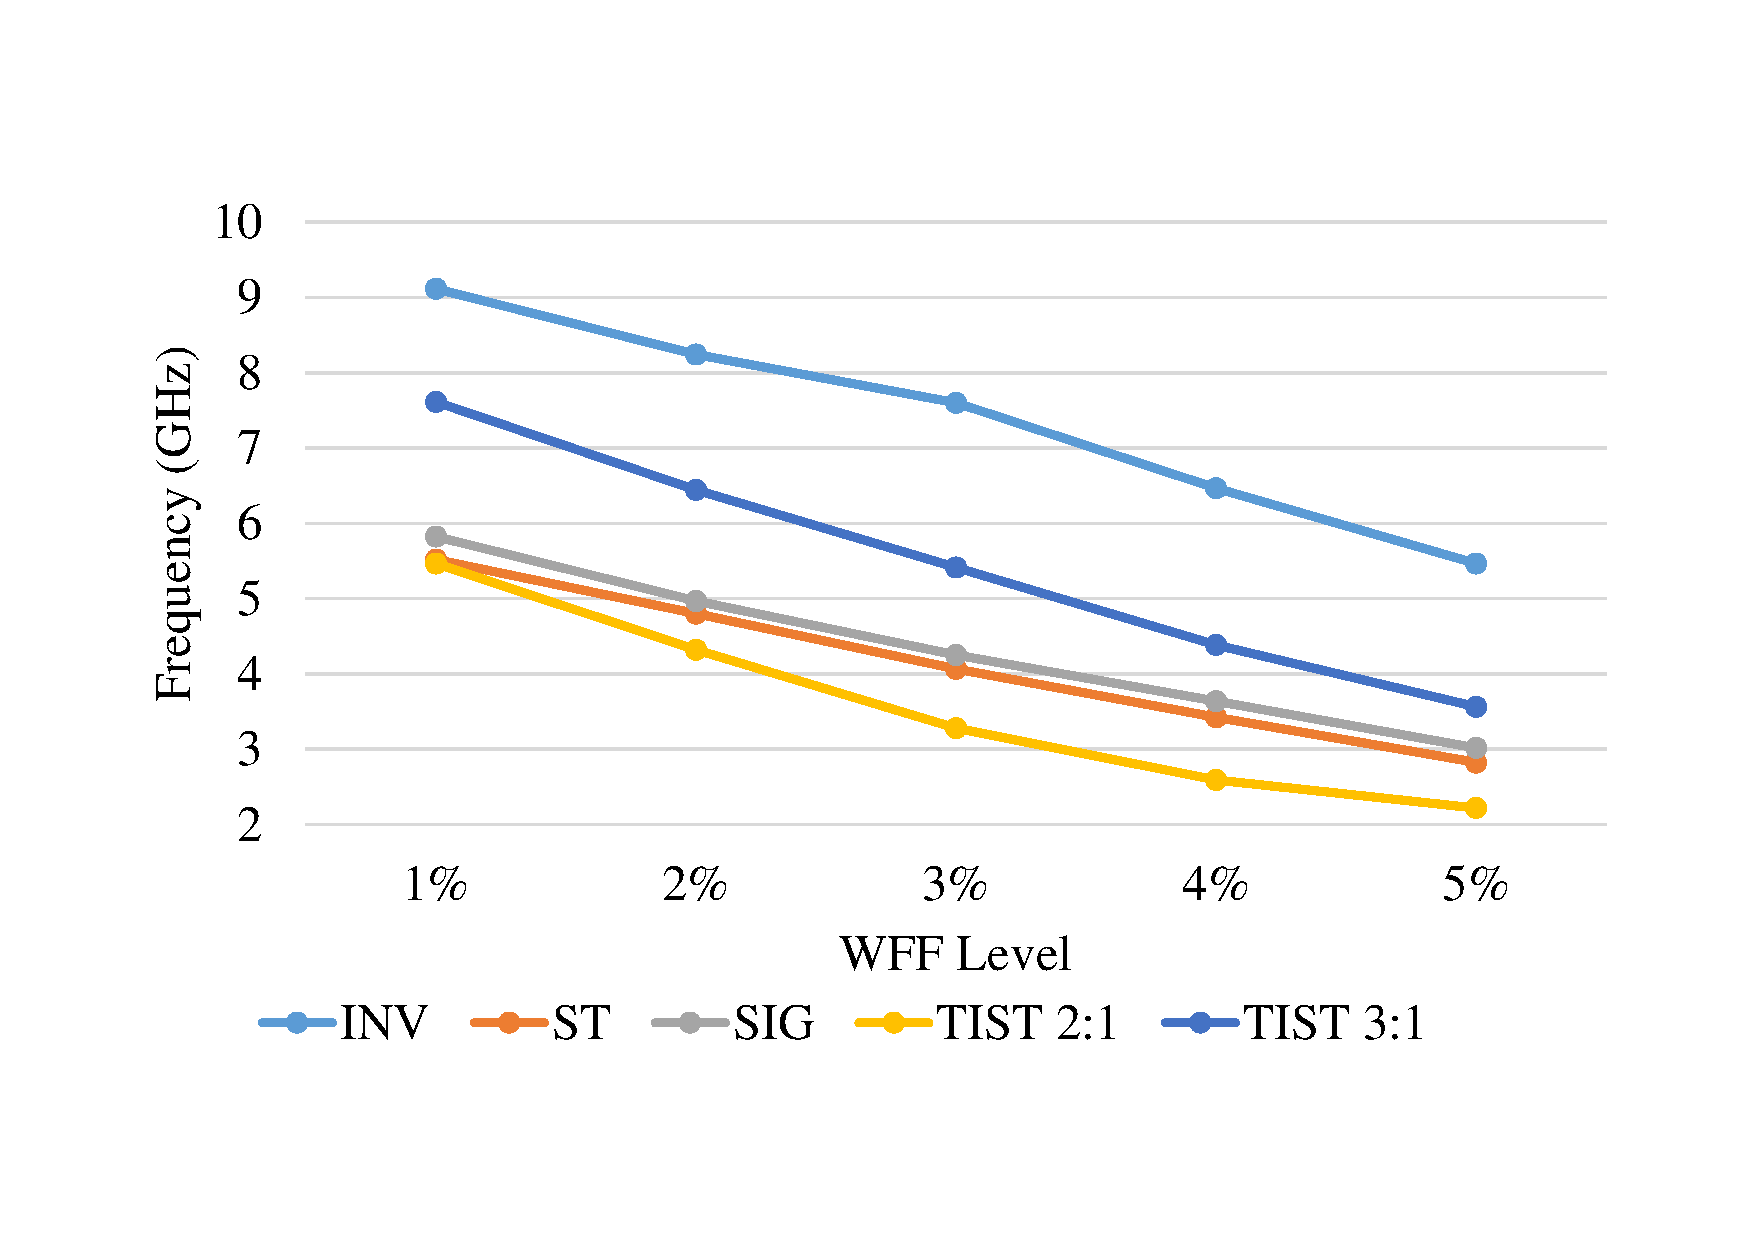
\includegraphics[width=0.8\textwidth, trim={2cm 3cm 2cm 3cm},clip]{freqRetWFF.pdf}
\caption{Frequency decrease over variability scaling for each design.}
\label{fig:freqRetWFF}
\legend{Source: From the author.}
\end{figure}

When isolating the influence of the number of fins and supply voltage over the frequency behavior over variability, it can be observed clear advantages for sizings above 1 fin and supply voltages above 300mV. From 1 fin to 2 fins it was observed an increase of 10.62\% over frequency retention, although above 2 fins, the increase on retention for each extra fin kept steady at 0.77\%. For the supply voltage, each 100mV increase from 0.1V to 0.3V increased the frequency retention by 3.66\%, while each 100mV increase from 0.3V to 0.7V improved the frequency retention by 13.79\%, on average. Given so, if performance is a priority, the number of fins should be kept above 2, and if trying to improve robustnes, the increase of supply voltage from 100mV to 300mV will not provide considerable gains.

%\vspace{-1cm}

\section{Propagation Times}

\vspace{-0.5cm}

Related to the frequencies, the propagation times will deviate according to the threshold voltages variations and its effects into the currents. Propagation times deviations will directly influence the circuit frequency, increasing the time guardband necessary in order to include the worst cases at the circuit frequency.

Given so, propagation times deviations for each design, in comparison to the inverter was 36.36\% and 43.21\% lower, for the ST and SIG, while the TIST 2:1 and 3:1 designs presented 72.89\% and 103.26\% higher deviations, as shown in Fig. \ref{fig:delaysDev}. This results is calculated considering the normalized deviation for all scenarios, even the ones where the design did not work properly, in order to not deflate the results for the TIST designs.

Calculating the average normalized devations only considering the cases where each design worked properly puts the inverter at the lowest normalized deviation while the ST, SIG, TIST 2:1, and TIST 3:1 presented 8.54\%, 7.04\%, 146.15\%, and 36.28\% higher sensibilities. By calculating the average normalized deviation this way, a fair comparison ban be made between the designs, given that onlythe subset of scenarios where all designs worked is considered.

\begin{figure}[h]
	\centering
		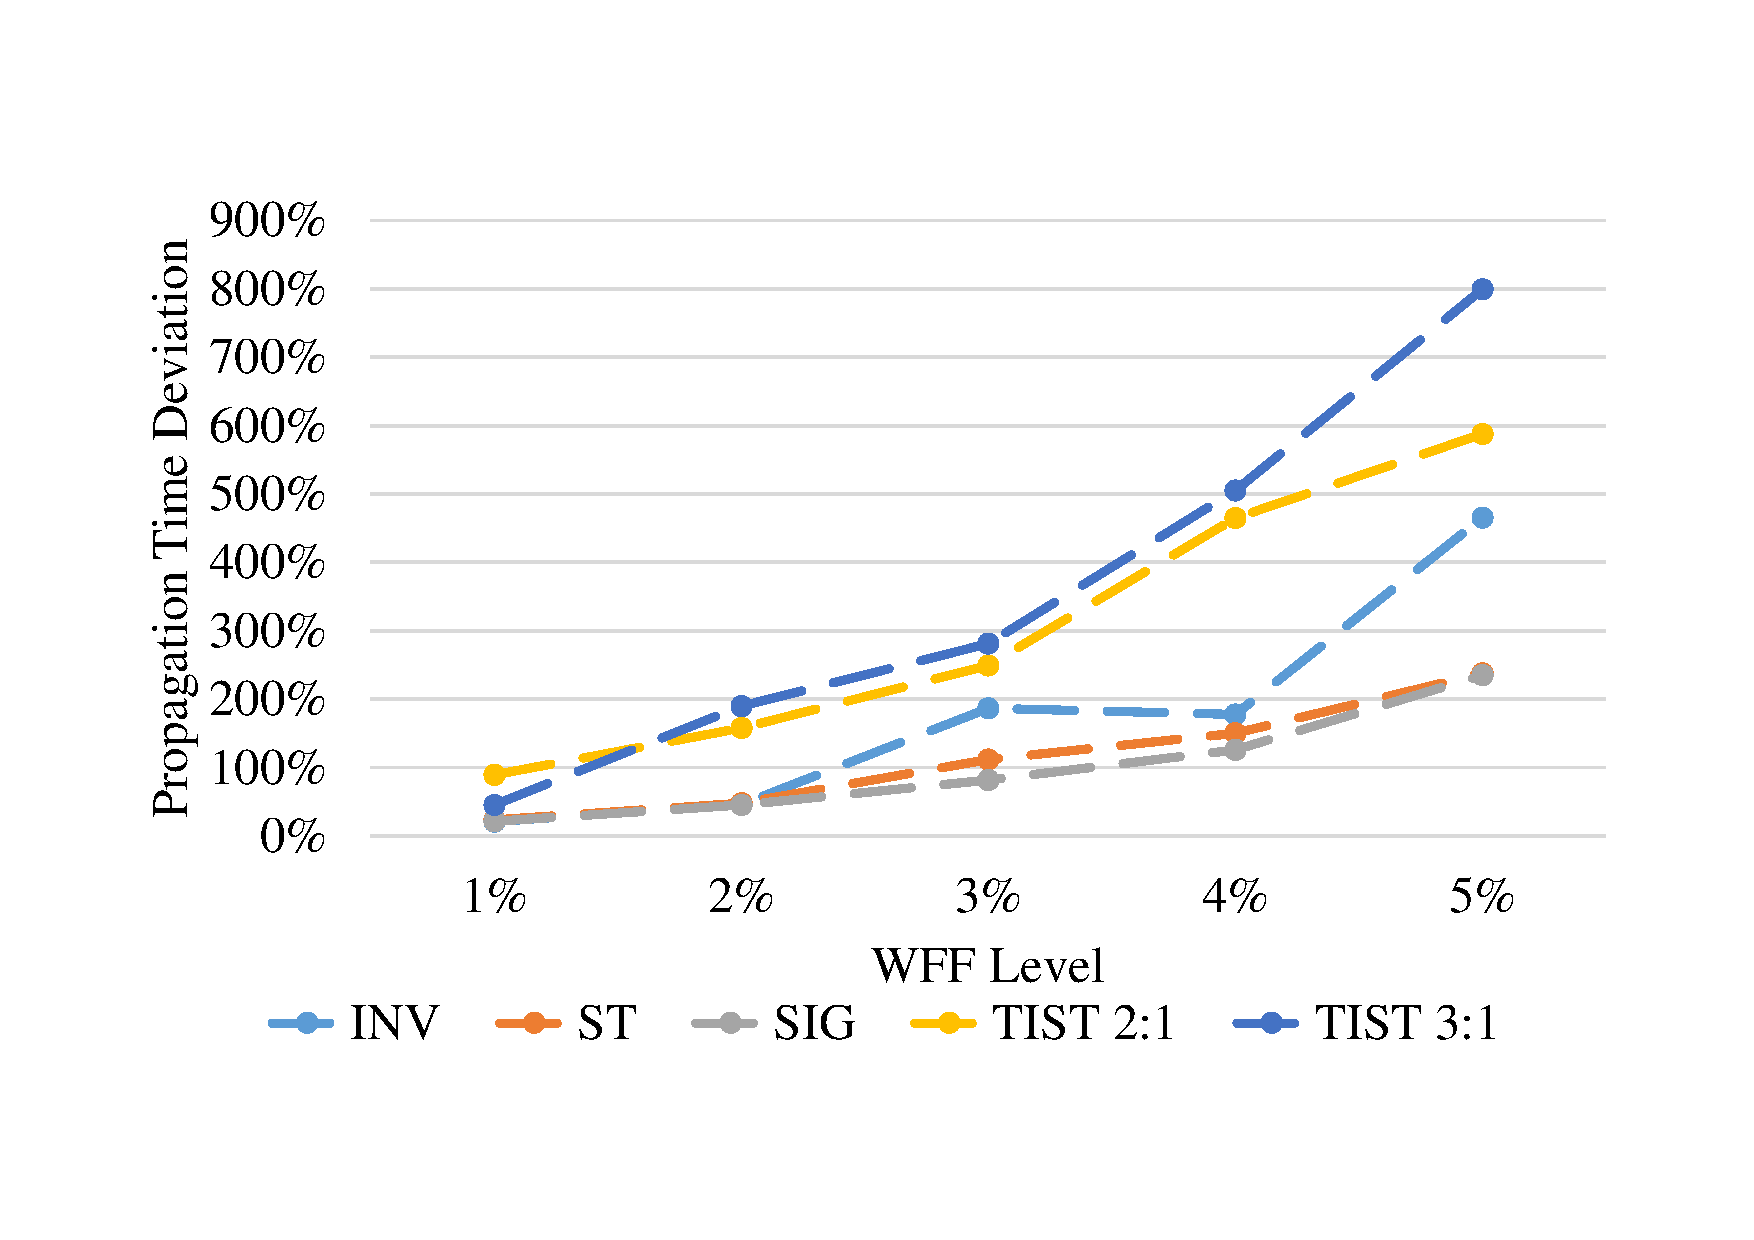
\includegraphics[width=0.8\textwidth, trim={2cm 3cm 2cm 3cm}, clip]{delayDevWFF.pdf}
		\caption{Propagation times deviation for each design in relation to the WFF level considering all scenarios.}
	\label{fig:delaysDev}
       	\legend{Source: From the author.}
\end{figure}

\section{Energy Consumption and Deviation}

For a circuit operating on a battery-oriented application or even, making use of energy harvesting methods to power itself up, the energy consumption should be stable. Deviation into energy consumption will influence the device battery-life and even leave energy-harvesting circuits non-operational. In addition, the energy consumption absolute value should be as minimal as possible, in order to preserve battery lifetime and make energy-harvesting methods feasible.

Among the considered inverter designs, when comparing average energy consumption measures for the scenarios where each design worked properly, the ST and SIG presented 173.07\% and 50.74\% higher energy consumptions than the inverter, while the TIST 2:1 and 3:1 designs presented 480.68\% and 310.83\% increases. With energy being a factor of propagation times (and consequently the frequency) and power drawn from the supply rails, there are factors which will specifically influence the circuit propagation times or the power consumption. Influencing the propagation times, there is the transistor count, increasing the circuits parasitics which increases its time to properly charge/discharge its signal and, for the circuits that present it, the hysteresis effects will make the circuit take longer to chage its output value, decreasing its frequency. And influencing the power consumption, a by-product of how much current is being drawn from the supply rail, there are how much fins the transistors have and how much paths from source to ground there are.

When comparing the average energy consumption measures for all scenarios, in comparison to the inverter, the ST and SIG presented 174.21\% and 95.84\% higher energy consumption, while the TIST 2:1 and 3:1 designs presented 1303.38\% and 993.77\% increases. This result shows the much higher impact of variability in the cases where the circuits could not work at the minimum frequency, for the SIG and TISTs designs. Given the larger transistor count, the hysteresis effect, and the number of paths from source to ground, it is expected an ascending increase from the inverter, SIG, ST and TIST designs energy consumption.

Isolating each variable, the impact of each extra fin start from a maximum of 145.75\% increase from 1 to 2 fins to 18.7\% from 4 to 5 fins, with diminishing energy increases alongside the number of fins. The higher increase at a lower number of fins is due to the higher relative increase in transistor area, given that from 1 to 2 fins the area is doubled, while from 4 to 5 fins the area increases by 25\%, with the SIG presenting the lowest increase overall.

Considering each level of variability, in average, there was a maximum energy increase of 652.86\%. Although, this result is inflated due to two peaks in energy increase at 3\% and 5\% WFF level as shown in Fig. \ref{fig:energyWFFstep}. Those peaks are due to the increase in non-viable scenarios at each of the peaks WFF level. When considering only the viable scenarios, the energy increase for each WFF step is 15.16\%, 35.61\%, 20.94\%, 9.04\%, and 7.18\% for the inverter, ST, SIG, TIST 2:1 and 3:1, respectively.

\begin{figure}[h]
	\centering
		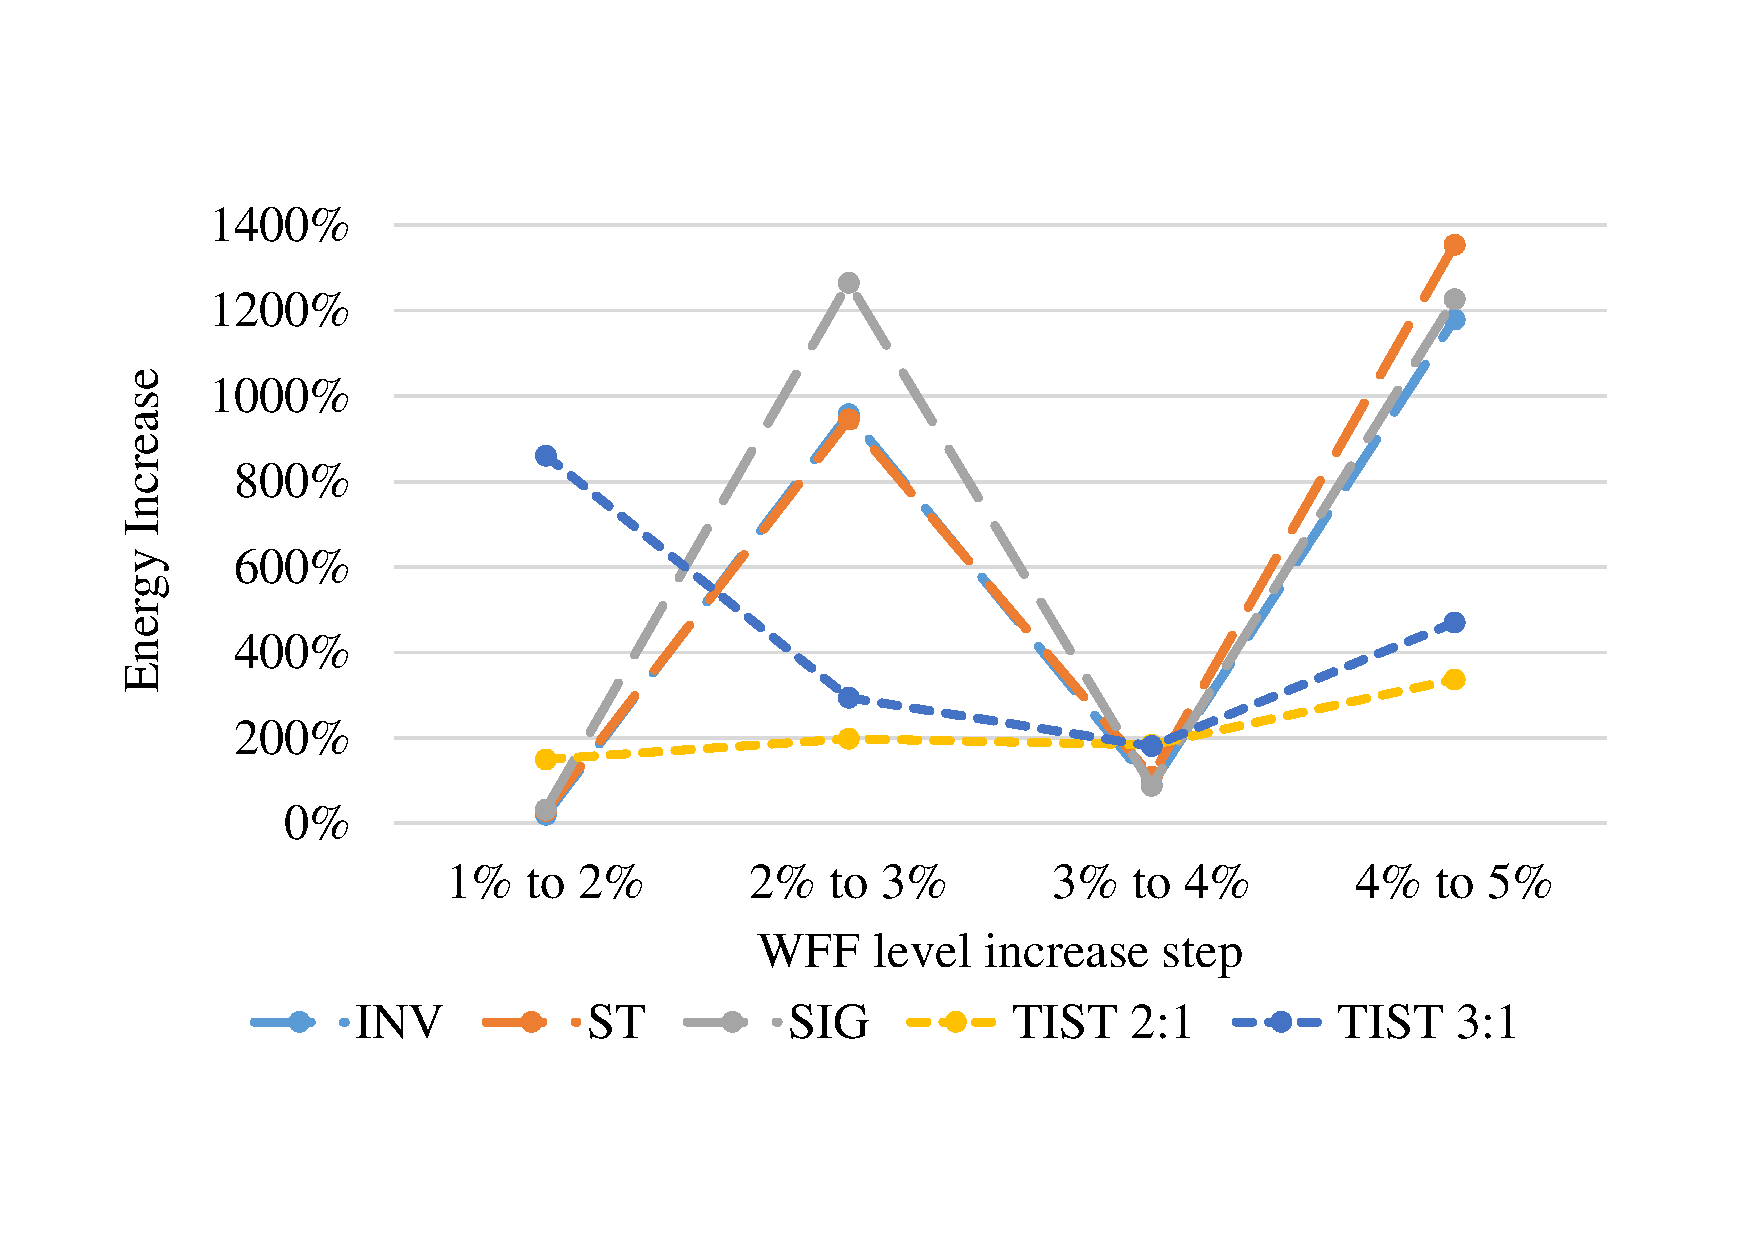
\includegraphics[width=0.8\textwidth, trim={2cm 3cm 2cm 3cm}, clip]{energyIncreaseWFFstep.pdf}
		\caption{Energy increase for each WFF level step.}
	\label{fig:energyWFFstep}
       	\legend{Source: From the author.}
\end{figure}

The impact of supply voltage on the energy consumption is shown at \ref{fig:energySupplyStep}. Highlighted in blue, for the inverter, ST, and SIG, and in red, for the TIST 2:! and 3:1, respectively, are the clusters of scenarios operating at the minimum frequency of 50KHz due to the variability impact. As shown, there are up to 2-order magnitude increases due to the decrease of supply voltage, revealing sub-300mV supply voltage operations to be highly susceptible to the variability effects.

%As a comparison, energy measures from simulations without inserted variability are shown at \ref{}.

\begin{figure}[h]
	\centering
		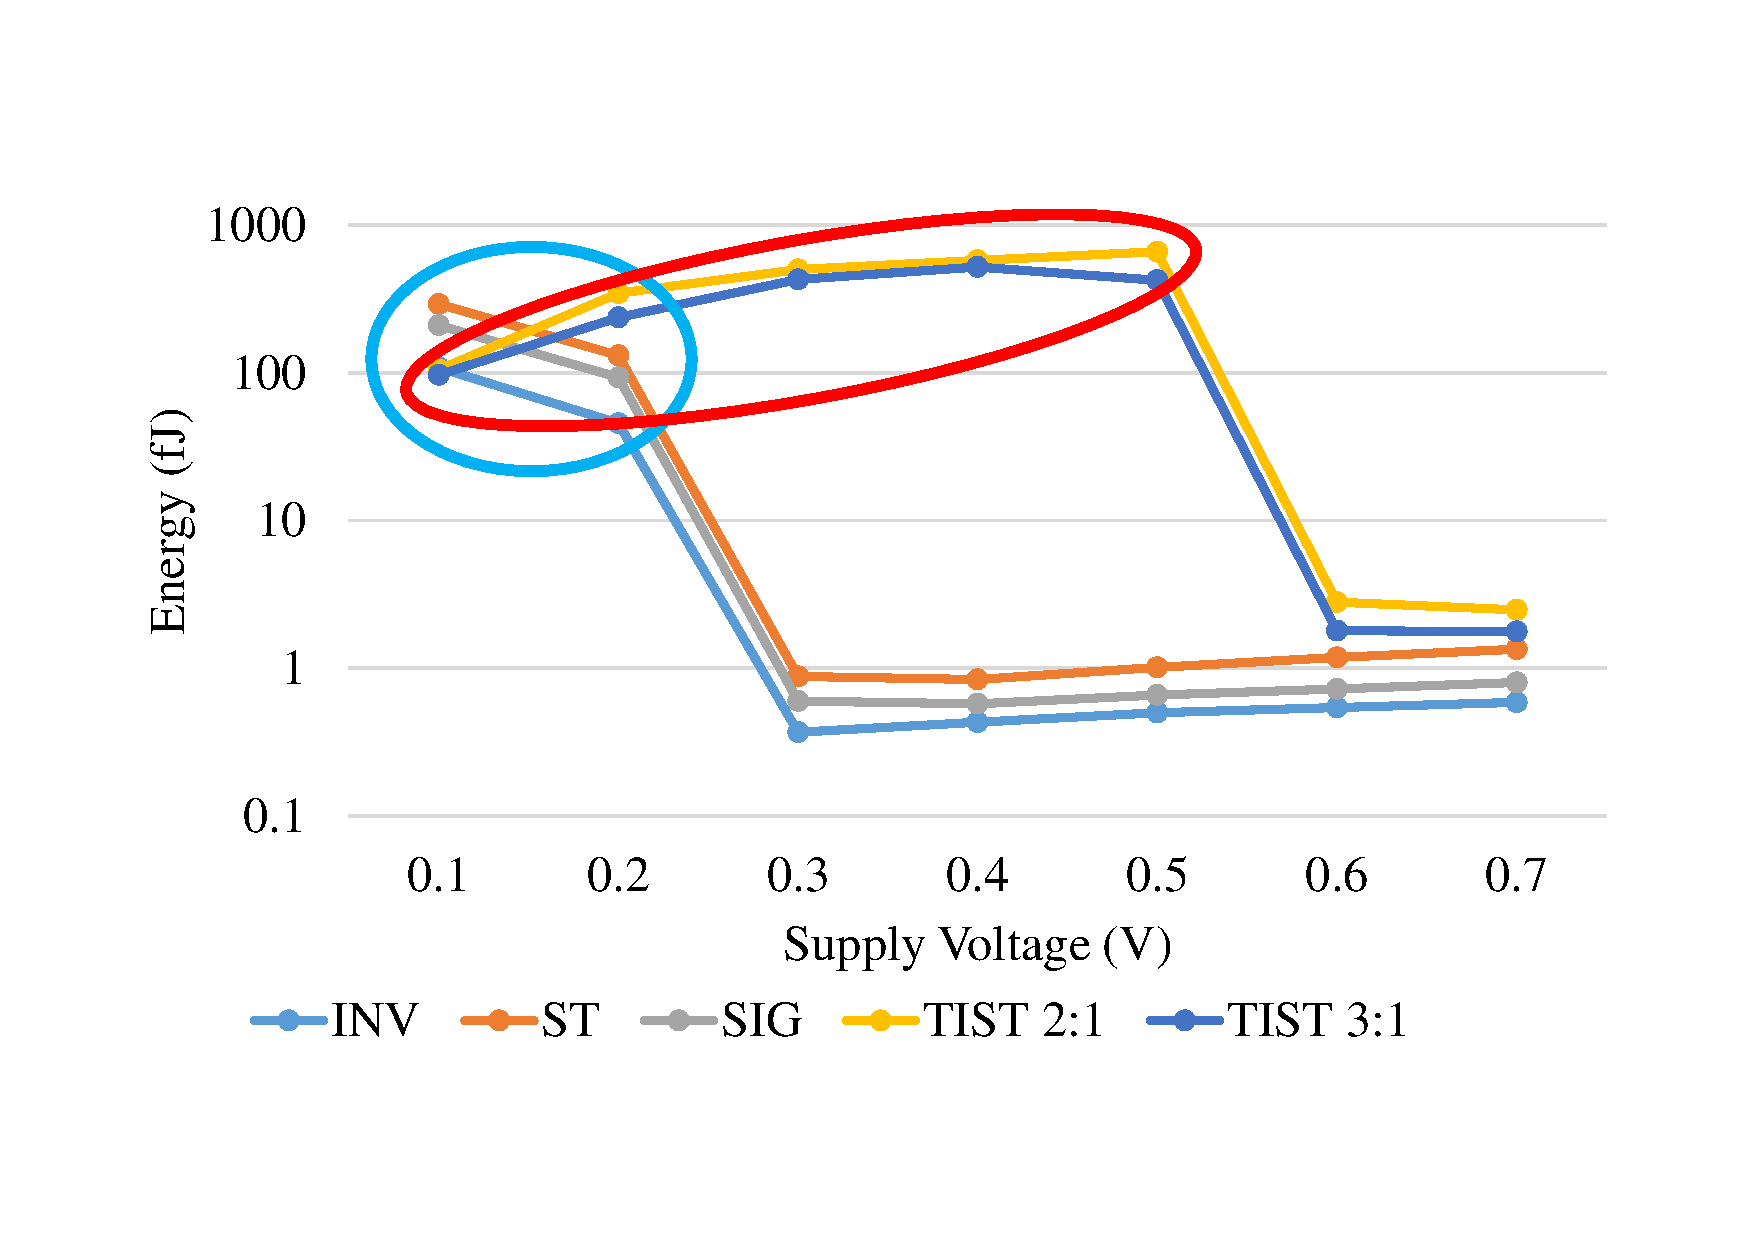
\includegraphics[width=0.8\textwidth, trim={2cm 3cm 2cm 3cm}, clip]{energyIncreaseSupply.pdf}
		\caption{Energy measures in function of the supply voltage for each design.}
	\label{fig:energySupplyStep}
       	\legend{Source: From the author.}
\end{figure}

%Concerning robustness, the ST and SIG presented a 55.83\%, 47.15\% higher sensibility while the TIST 2:1 and 3:1 presented a 42.39\% and 52.03\% lower sensibility to the process variability impact in comparison to the traditional inverter considering the scenarios where each design presented acceptable behavior. In order to make a fair comparison, considering only the subset of scenarios where all designs worked properly, the ST and TIST 3:1 presented 1.13\% and 33.36\% lower sensibilities while the SIG and TIST 2:1 presented 5.5\% and 7.99\% higher variability sensibility. Additionally, considering all cases, even when the circuit did not work properly, the ST, SIG, TIST 2:1, and TIST 3:1 presented 19.85\%, 12.09\%, 145.96\%, and 118.24\% higher sensibilities in comparison to the traditional inverter.

%The energy consumption increase over each variability scenario kept stable over 15.16\%, 35.6\%, 20.94\%, 9.04\% and, 7.18\% for the inverter, ST, SIG, TIST 2:1 and, TIST 3:1, respectively. Such increase is related to the frequency decrease over variability scaling. The low increase related to the TIST designs is due to many of the low supply voltage scenarios not being taken into account, in comparison to the other designs, since it did not work properly. A more fair analysis would consider only the subset of cases where all designs worked properly. Given such subset, the energy increase over each variability scenario would be 17.59\%, 18.16\%, 18.62\%, 9.04\% and 11.59\% for the inverter, ST, SIG, TIST 2:1 and, TIST 3:1, respectively.
    %Energy consumption measures over variability scenarios for each design is shown at Figure \ref{figEnergiaAbs}.


    %Which, as stated before, is expected.

    %\begin{figure}[b]
    %    \centering
    %        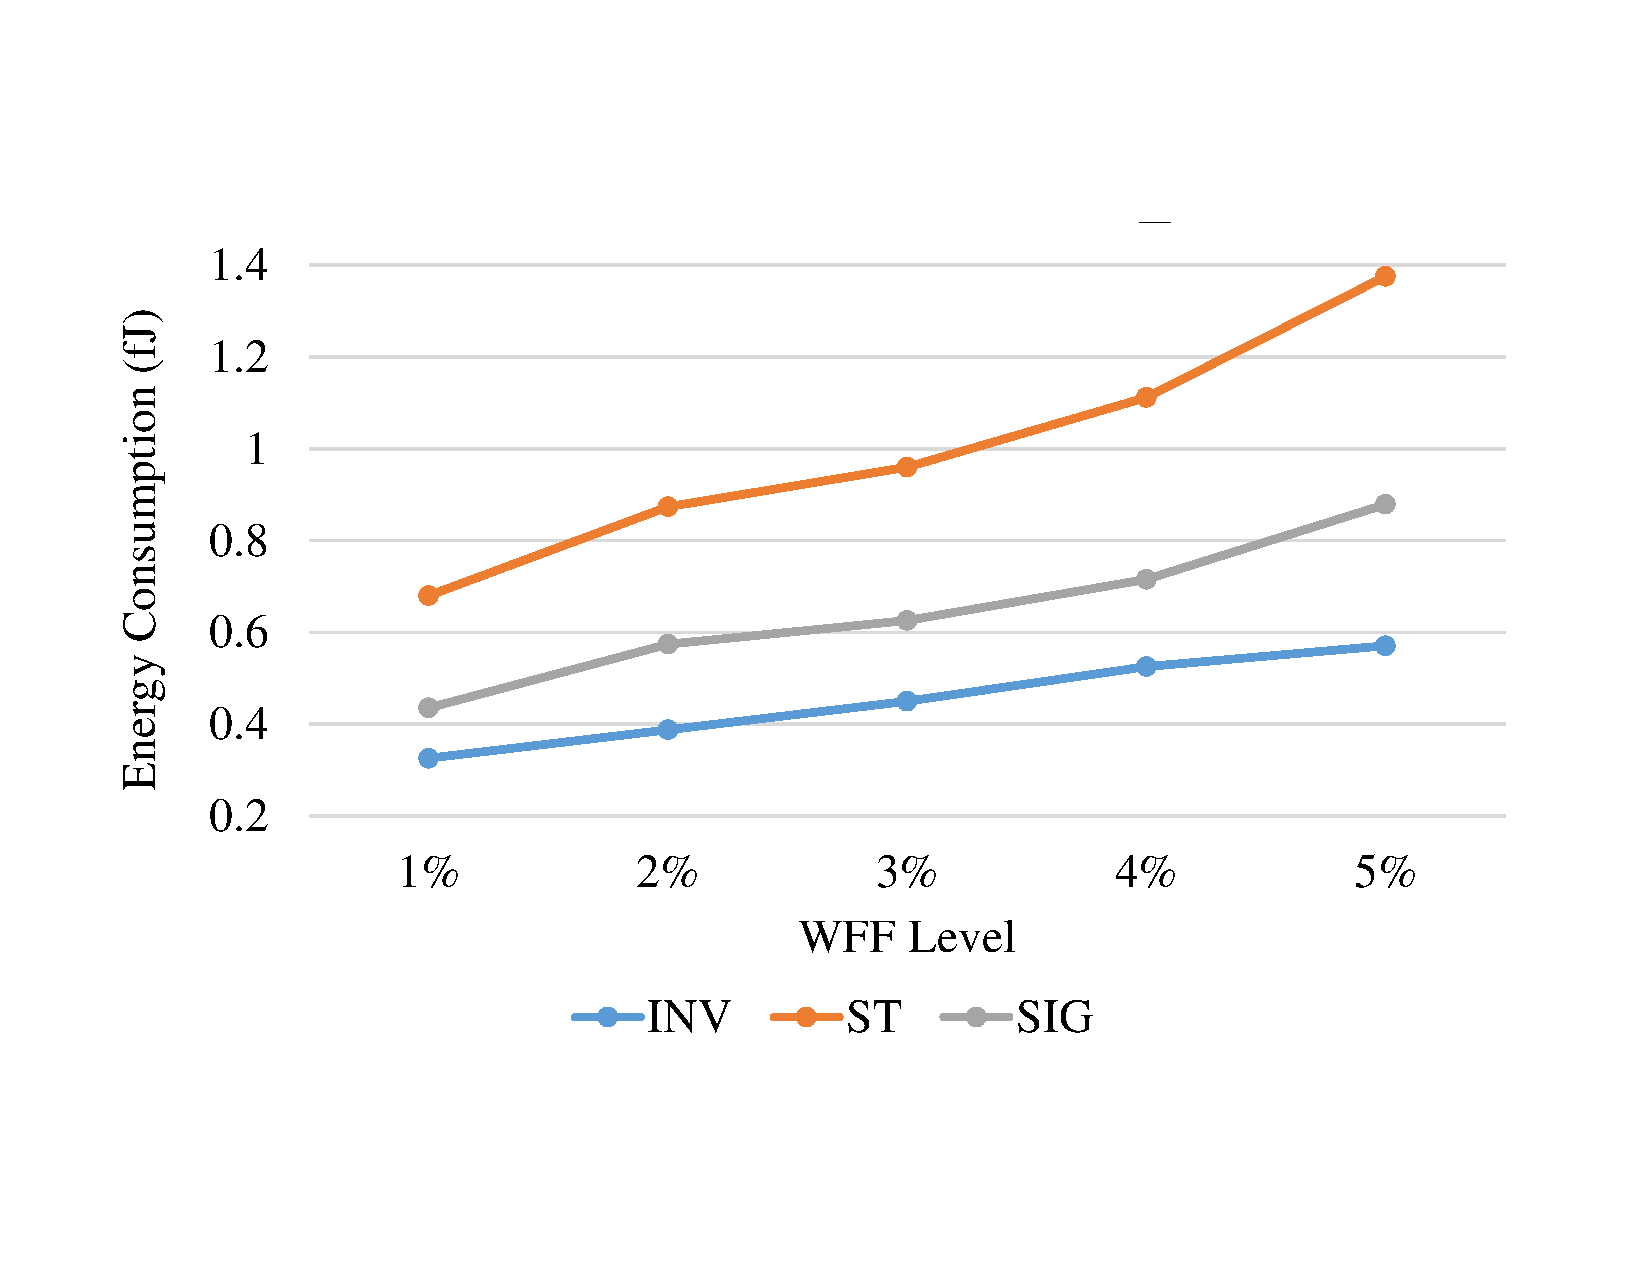
\includegraphics[width=0.45\textwidth, trim={2cm 4cm 2cm 4cm}, clip]{compEnergiaAbs.pdf}
            %\caption{Energy consumption increase over variability scaling.}
   %     \label{figEnergiaAbs}
  %  \end{figure}


	Depending on the focus of the application, there could be several kinds of objectives. Overall, for low power applications, the focus should be on circuit designs directives to achieve circuits with the minimum energy consumption possible. Much of these directives aims for the decrease of currents, like the increase of the transistors channel length and the decrease of supply voltages. Although, such techniques will further decrease the circuits robustness to the effects of variability and radiation.

Given so, trying to achieve a balance between given applications three types of analysis were performed, where the most apropriate subset of characteristics involving transistor sizing and supply voltage for each level of process variability is identified for the 1) lowest energy consumption, 2) highest robustness to the effects of process variability and 3) the most Cost-Benefit (CB). The lowest energy layout is identified through the energy measures. The higher robustness layout is identified by the lowest normalized standard deviation concerning energy consumption, and the CB layout is identified by the lowest value considering the product between the energy consumption and normalized standard deviation (EDP - Energy Deviation Product). The results are shown at Table \ref{tab:3types}. Some results will show more than one appropriate layout/supply voltage in order to provide flexibility, considering values up to 5\% higher than the minimum considered value.

\begin{table}[]
\centering
\caption{Recommended layout and supply voltage for each design and variability level.}
\label{tab:3types}
\resizebox{\textwidth}{!}{
\begin{tabular}{|c|c|c|c|c|c|c|c|}
\hline
\multirow{2}{*}{Design} & \multirow{2}{*}{WFF} & \multicolumn{2}{c|}{Minimum Energy} & \multicolumn{2}{c|}{Highest Robustness} & \multicolumn{2}{c|}{CB} \\ \cline{3-8}
                          &     & Supply (V) & \#Fins & Supply (V) & \#Fins       & Supply (V) & \#Fins \\ \hline
\multirow{5}{*}{INV}      & 1\% & 0.1        & 1 or 2 & 0.7        & 1            & 0.7        & 1      \\ \cline{2-8}
                          & 2\% & 0.1        & 1      & 0.3        & 4 or 5       & 0.2        & 2 to 4 \\ \cline{2-8}
                          & 3\% & 0.2        & 1      & 0.3        & 5            & 0.3        & 3 to 5 \\ \cline{2-8}
                          & 4\% & 0.3        & 1 or 2 & 0.4        & 5            & 0.4        & 5      \\ \cline{2-8}
                          & 5\% & 0.3        & 1      & 0.4        & 1       	  & 0.4        & 1      \\ \hline
\multirow{5}{*}{ST}       & 1\% & 0.1        & 1      & 0.7        & 5            & 0.7        & 1      \\ \cline{2-8}
                          & 2\% & 0.2        & 1      & 0.7        & 5            & 0.7        & 1      \\ \cline{2-8}
                          & 3\% & 0.2        & 1      & 0.7        & 4 or 5       & 0.3        & 1      \\ \cline{2-8}
                          & 4\% & 0.3        & 1      & 0.4        & 2            & 0.4        & 1 or 2 \\ \cline{2-8}
                          & 5\% & 0.4        & 1      & 0.5        & 2 to 5       & 0.5        & 1 or 2 \\ \hline
\multirow{5}{*}{SIG}      & 1\% & 0.1        & 1      & 0.7        & 2            & 0.7        & 1      \\ \cline{2-8}
                          & 2\% & 0.2        & 1      & 0.3        & 3 or 4       & 0.7        & 1      \\ \cline{2-8}
                          & 3\% & 0.2        & 1      & 0.3        & 3            & 0.3        & 1      \\ \cline{2-8}
                          & 4\% & 0.3        & 1      & 0.4        & 3            & 0.4        & 2 or 3 \\ \cline{2-8}
                          & 5\% & 0.4        & 1      & 0.5        & 2 or 3       & 0.5        & 2      \\ \hline
\multirow{5}{*}{TIST 2:1} & 1\% & 0.1        & 2F1F   & 0.7        & 4F2F         & 0.7        & 2F1F   \\ \cline{2-8}
                          & 2\% & 0.1        & 2F1F   & 0.6        & 4F2F         & 0.6        & 2F1F   \\ \cline{2-8}
                          & 3\% & 0.7        & 2F1F   & 0.6        & 2F1F         & 0.6        & 2F1F   \\ \cline{2-8}
                          & 4\% & 0.7        & 2F1F   & 0.7        & 4F2F         & 0.7        & 2F1F   \\ \cline{2-8}
                          & 5\% & 0.7        & 2F1F   & 0.7        & 6F3F         & 0.7        & 2F1F   \\ \hline
\multirow{5}{*}{TIST 3:1} & 1\% & 0.1        & 3F1F   & 0.7        & 6F2F         & 0.7        & 3F1F   \\ \cline{2-8}
                          & 2\% & 0.1        & 3F1F   & 0.7        & 6F2F or 3F1F & 0.7        & 3F1F   \\ \cline{2-8}
                          & 3\% & 0.7 or 0.6 & 3F1F   & 0.6 or 0.7 & 6F2F or 3F1F & 0.7        & 3F1F   \\ \cline{2-8}
                          & 4\% & 0.7 or 0.6 & 3F1F   & 0.6        & 6F2F         & 0.6        & 3F1F   \\ \cline{2-8}
                          & 5\% & 0.7 or 0.6 & 3F1F   & 0.6        & 3F1F         & 0.6        & 3F1F   \\ \hline
\end{tabular}
}
\end{table}

	It is possible to identify patterns concerning the minimum energy and highest robustness layouts. The minimum energy layouts, as a general rule, will contain only few fins, if not only one, and lower supply voltages. Both low values aim to lower currents and increase resistance, therefore decreasing energy consumption. As variability rises, the supply voltage rises as well. That is due to the lower frequencies applied in those scenarios and the consequent increase on propagation times, given that energy is the by-product of power and time. A higher supply voltage will decrease propagation times followed by a decrease on energy consumption. The TIST designs present a steep increase on supply voltage, from 0.1V to 0.6V/0.7V due to the lack of possible mid-term (0.2V to 0.5V) viable scenarios.

    The robust layouts present a shift on supply voltage. At low variability scenarios (1\% to 3\%) the nominal supply voltage will persist at nominal value (0.7V). As the variability level rises, the supply voltage will abruptly fall into near-threshold region (300mV to 400mV) and increase as the variability level increases as well.

	The sudden fall into a near-threshold region can be explained in terms of the transistors current. When the on-current is at the saturation region, it presents an quadratic dependency over the $V_{T}$, as shown in equation \ref{eqn:sat}, while at the linear region, the on-current presents a linear dependency over the $V_{T}$, as shown in equation \ref{eqn:lin} \cite{van2004principles}. Given so, as the level of variability rises, the transistor will have to fall into linear region operation in order to decrease the current deviations due to increasingly $V_{T}$ variability.

    \begin{equation}
        \centering
        \label{eqn:sat}
        I_{D,sat} = \frac{\mu_p \cdot C_{ox}}{2} \cdot \frac{W}{L} \cdot (V_{GS} - V_T)^2
        \begin{cases}
        V_{GS} \leq V_T\\
        V_{DS} \leq V_{GS} - V_T
        \end{cases}
    \end{equation}
    \begin{equation}
        \centering
        \label{eqn:lin}
        I_{D,lin} = \frac{\mu_p \cdot C_{ox}}{2} \cdot \frac{W}{L} \cdot [2 \cdot (V_{GS} - V_T)V_{DS} - V_{DS}^2]
        \begin{cases}
        V_{GS} \leq V_T\\
        V_{DS} > V_{GS} - V_T
        \end{cases}
    \end{equation}
where:
\begin{conditions}
I_{D,sat} & saturation current \\
I_{D,lin} & linear current \\
\mu_p & p-material electron mobility \\
C_{ox} & specific capacitance of the gate \\
W & transistor width \\
L & transistor length \\
V_{GS} & gate-source voltage \\
V_{DS} & drain-source voltage \\
V_T & threshold voltage \\
\end{conditions}

For the CB layouts, what can be observed is an adoption of supply voltages similar to the high robustness layouts, with an earlier adoption of near-threshold supply voltages, as variability rises, and the adoption of a fin count similar to the low energy layouts, although slightly higher. Energy consumption and deviation comparisons between each recommended layout are shown in Fig. \ref{figscCompINV}, Fig. \ref{figscCompST}, Fig. \ref{figscCompSIG}, Fig. \ref{figscCompTIST21}, and Fig.\ref{figscCompTIST31}. The lines correspond to the energy consumption axis (left), while the bars correspond to the energy deviation axis (right).

    \begin{figure}[]
        \centering
        	\caption{Layout comparison for each scenario considering the energy metrics for the inverter.\label{figscCompINV}}
        	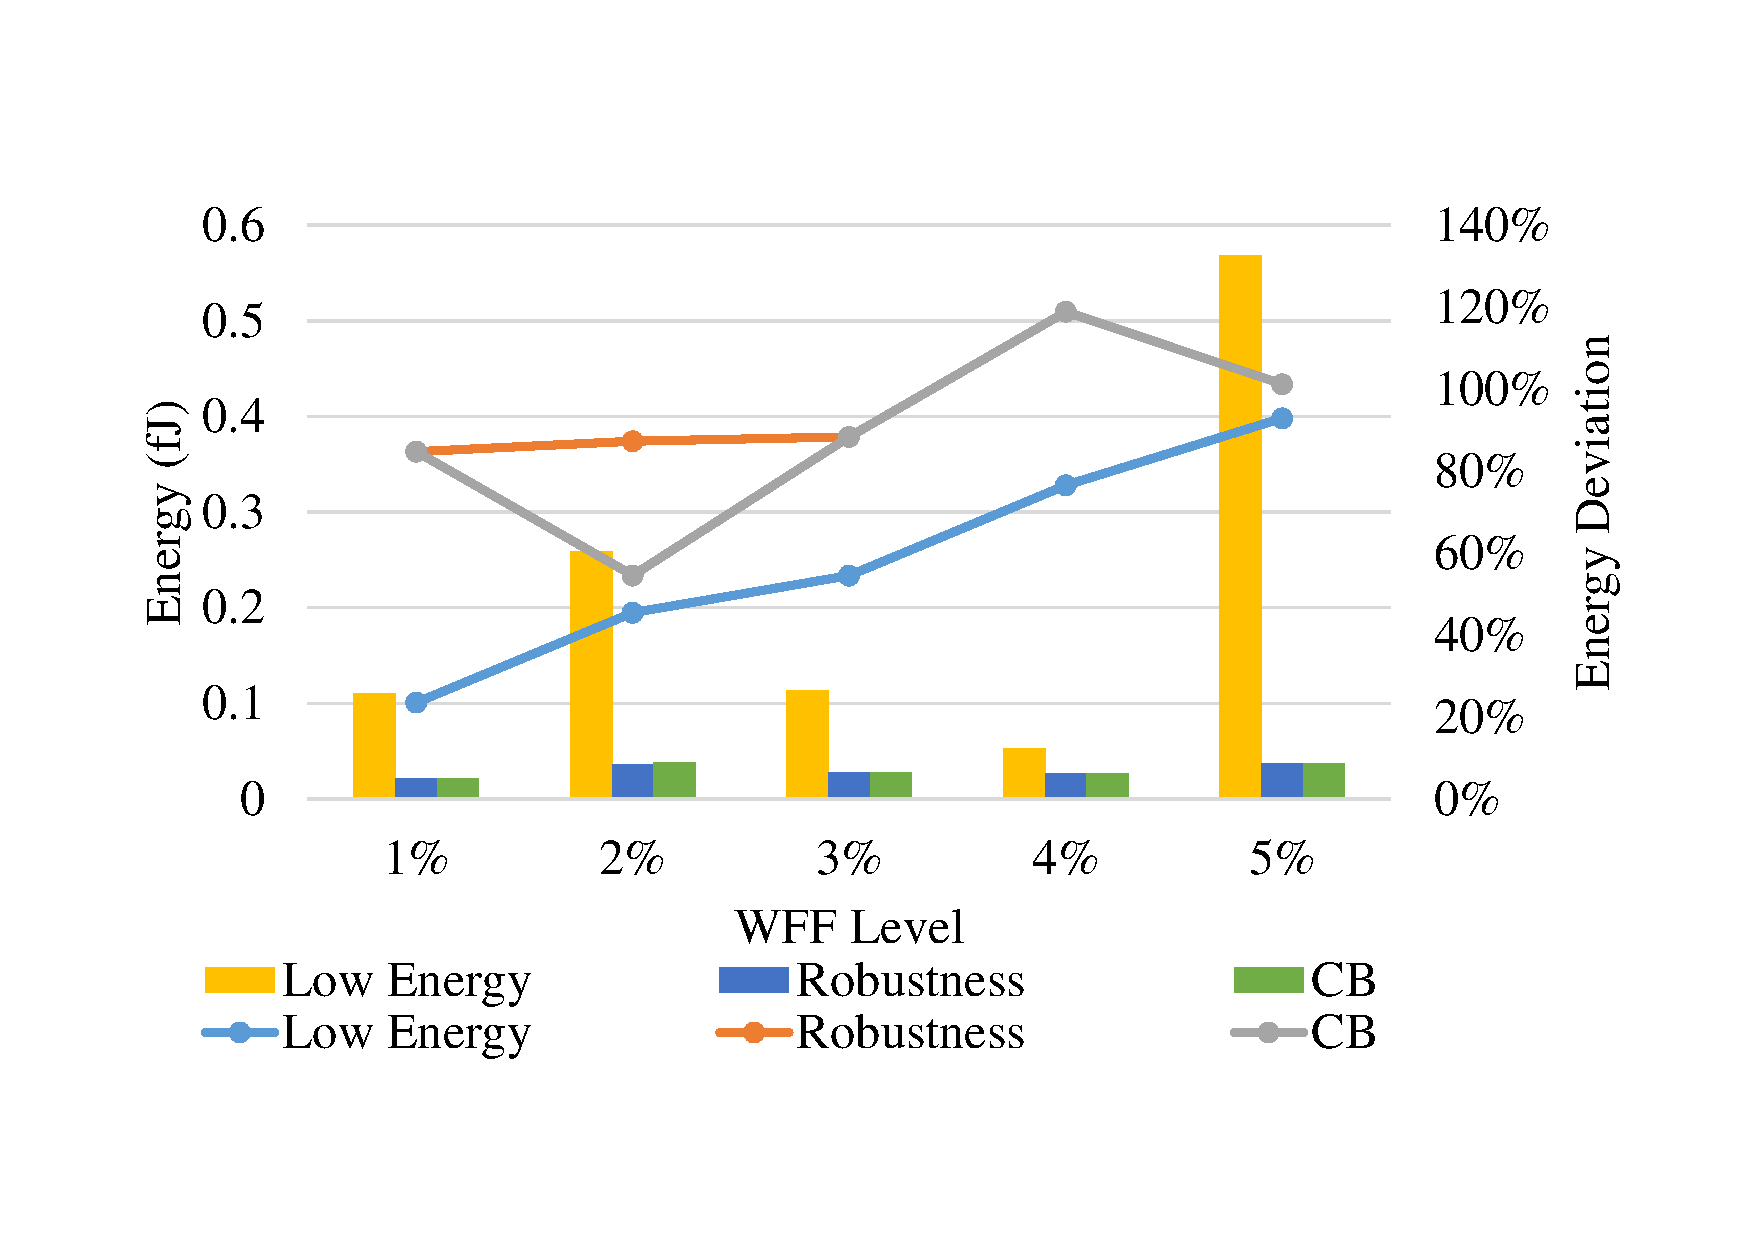
\includegraphics[width=0.9\textwidth, trim={1.25cm 2cm 2cm 3cm}, clip]{comp3Linv2Energy.pdf}
   \end{figure}

\begin{figure}[]
     \centering
            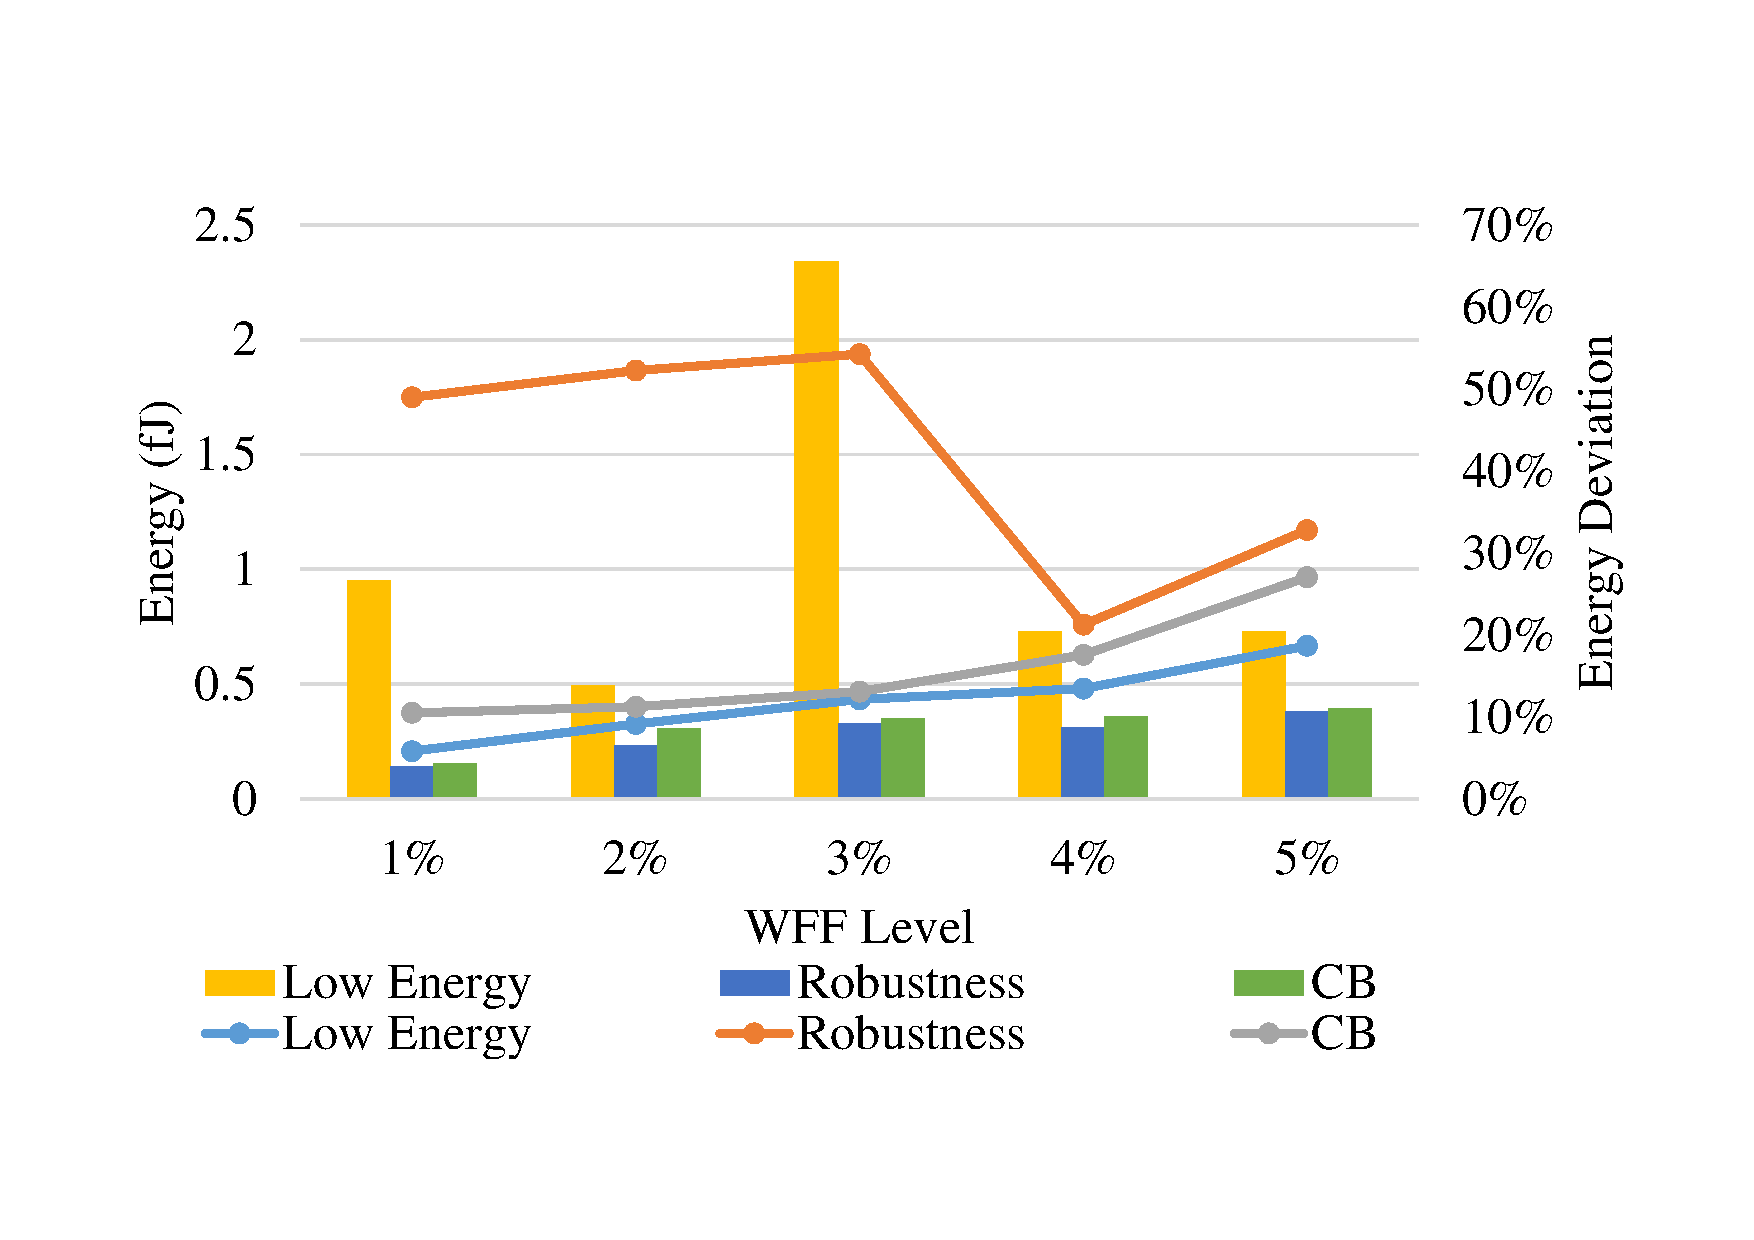
\includegraphics[width=0.9\textwidth, trim={1.25cm 3cm 2cm 3cm}, clip]{comp3Lst2Energy.pdf}
            \caption{Layout comparison for each scenario considering the energy metrics for the ST.\label{figscCompST}}
    \end{figure}

    \begin{figure}[]
        \centering
            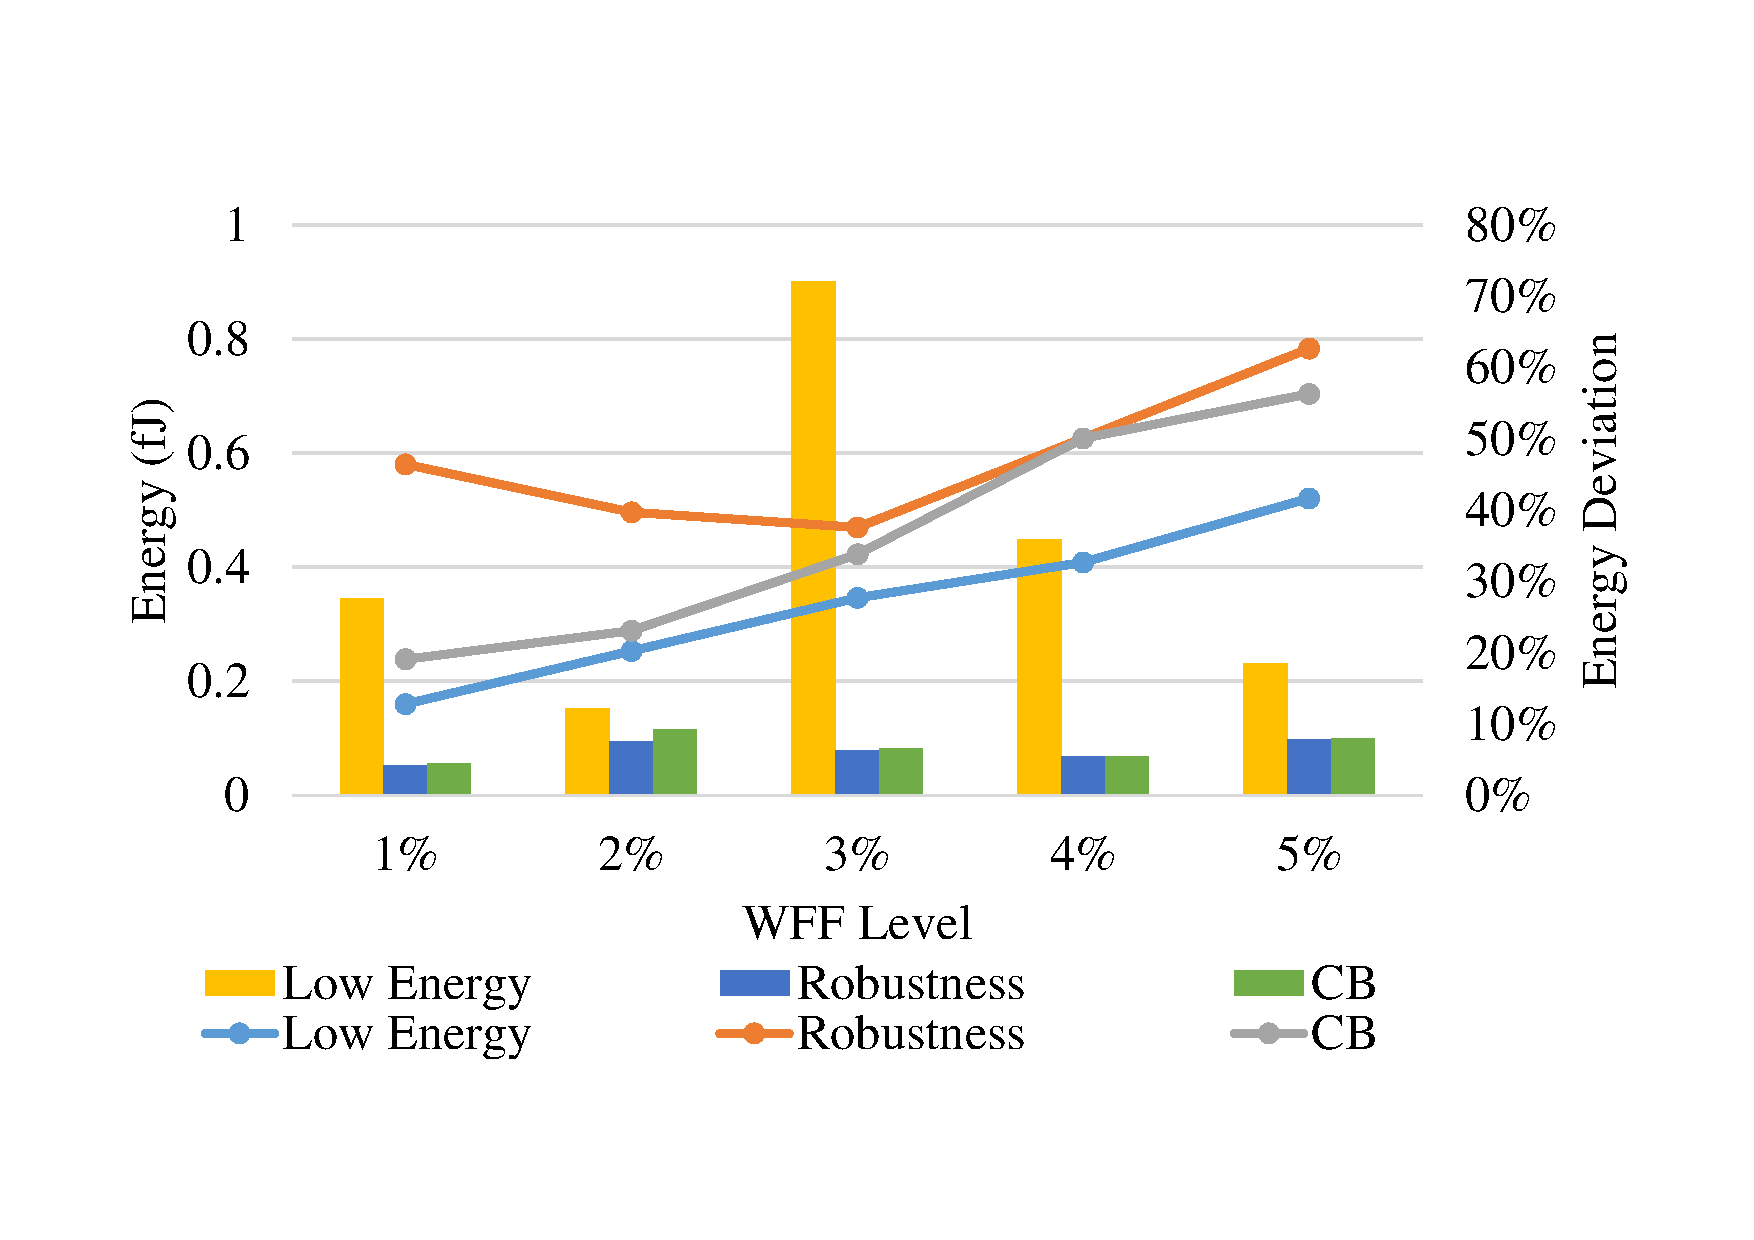
\includegraphics[width=0.9\textwidth, trim={1.25cm 3cm 2cm 3cm}, clip]{comp3Lsig2Energy.pdf}
            \caption{Layout comparison for each scenario considering the energy metrics for the SIG.}
        \label{figscCompSIG}
    \end{figure}

    \begin{figure}[]
        \centering
            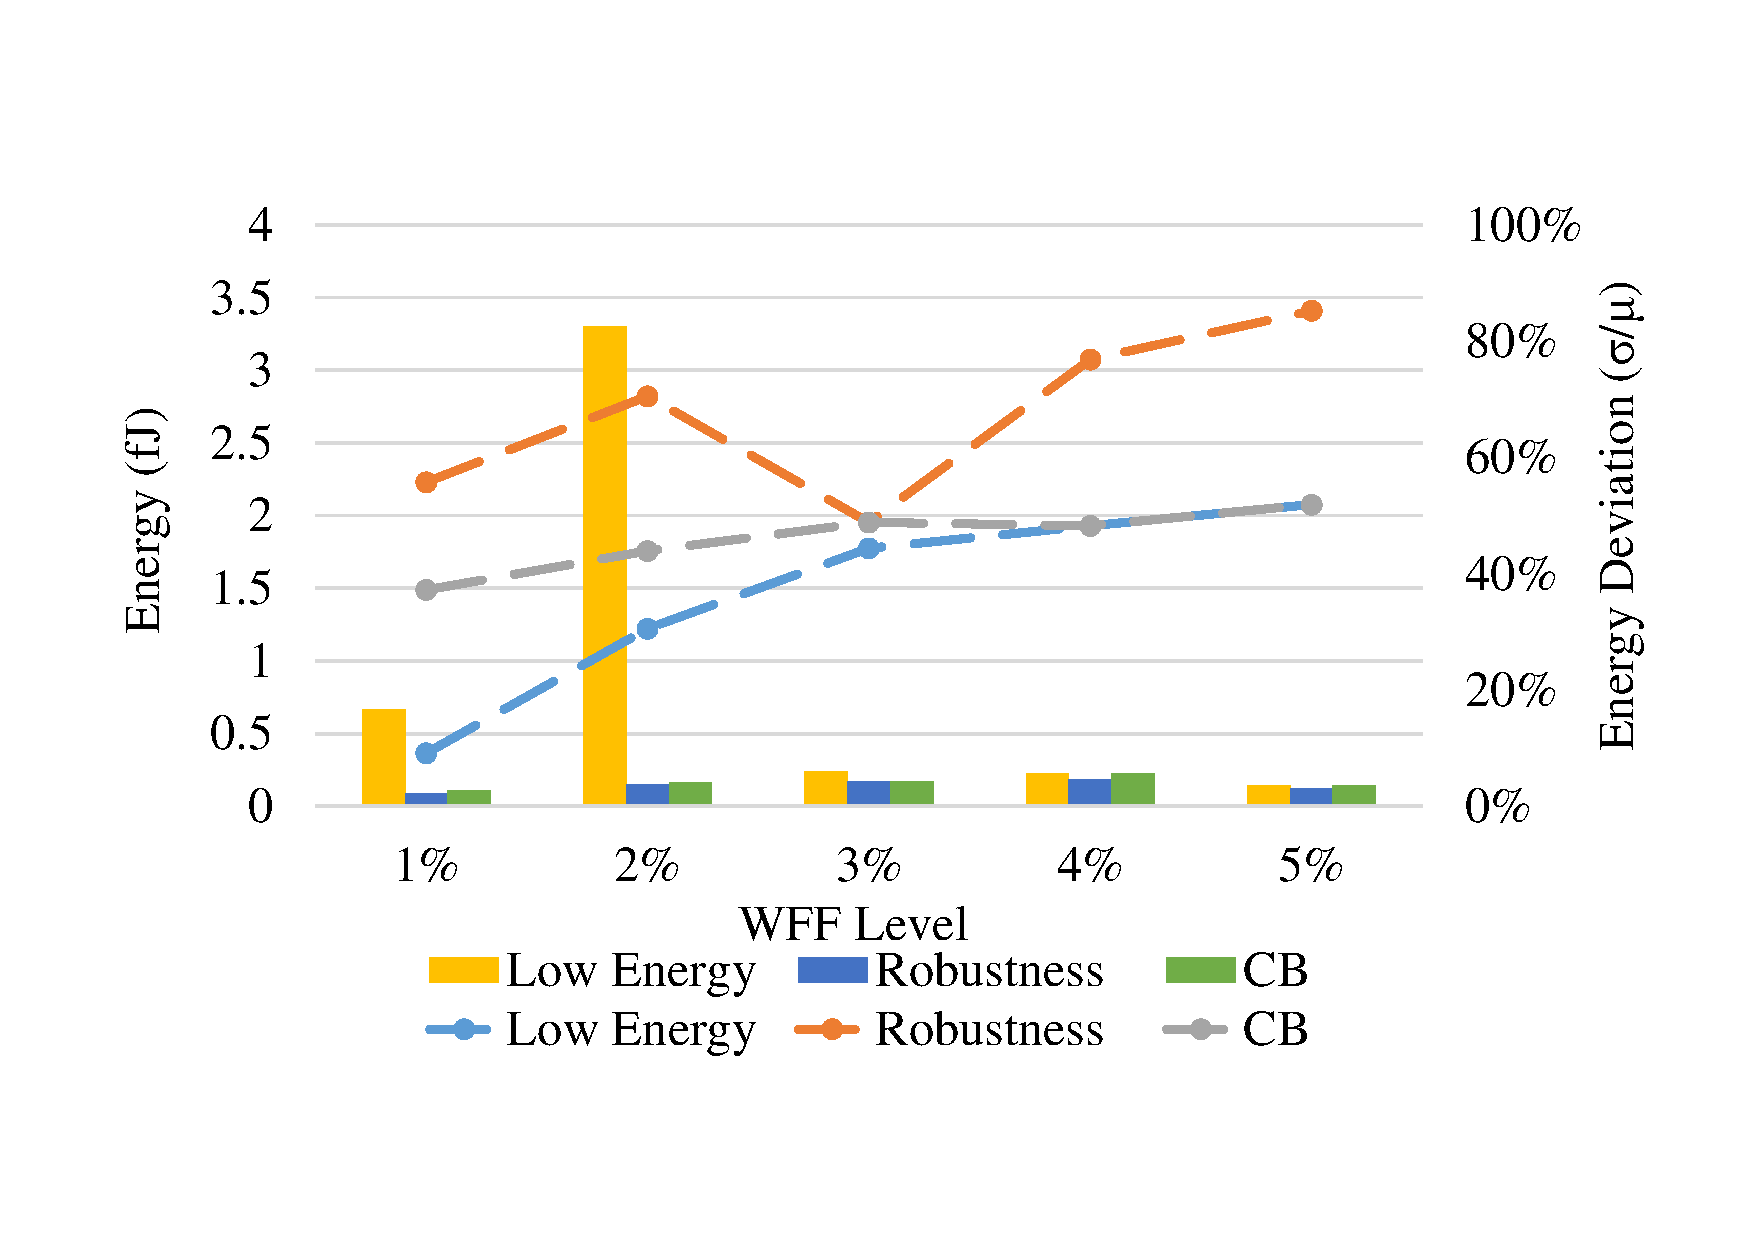
\includegraphics[width=0.9\textwidth, trim={1.25cm 3cm 2cm 3cm}, clip]{comp3Ltist212Energy.pdf}
            \caption{Layout comparison for each scenario considering the energy metrics for the TIST at 2:1 proportion.}
        \label{figscCompTIST21}
    \end{figure}

    \begin{figure}[]
        \centering
            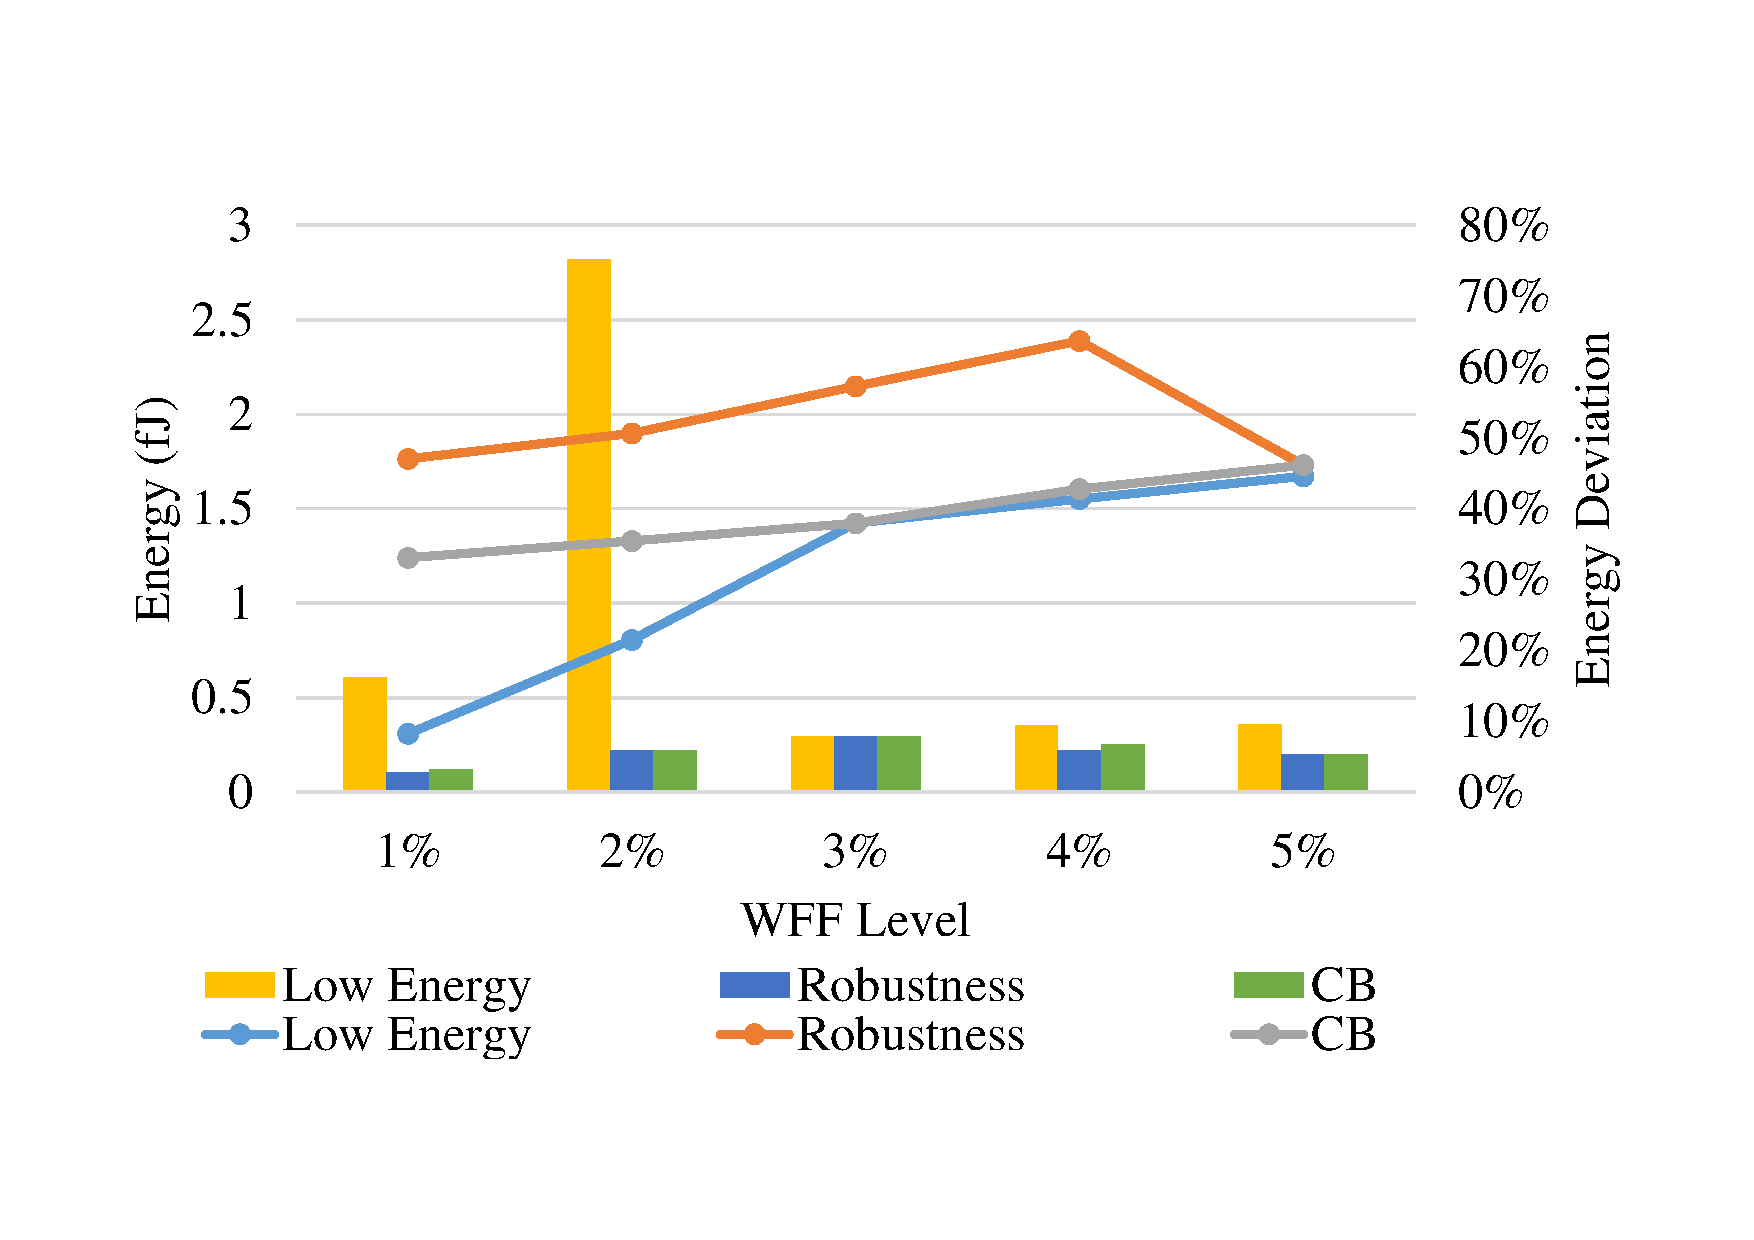
\includegraphics[width=0.9\textwidth, trim={1.25cm 3cm 2cm 3cm}, clip]{comp3Ltist312Energy.pdf}
            \caption{Layout comparison for each scenario considering the energy metrics for the TIST at 3:1 proportion.}
        \label{figscCompTIST31}
    \end{figure}

A further comparison between each design layout is presented in Fig. \ref{figCompLowEnergy}, Fig. \ref{figCompHighRobustness}, and Fig. \ref{figCompCB}. The lines correspond to the energy consumption axis (left), while the bars correspond to the energy deviation axis (right). Considering the averages, for the low energy layouts, the inverter presented the lowest energy consumption, followed by the SIG (34.61\% higher), ST (68.32\% higher), TIST 3:1 (358.84\% higher) and TIST 2:1 (487\% higher), respectively. The TIST layouts, showed the highest robustness, with the 2:1 variants presenting a 22.93\% average energy deviation and the 3:1 variants showing a minor increase with its 23.62\% average energy deviation. Following the TIST layouts, the ST, SIG and inverter present a 29.34\%, 33.25\%, and 51.55\% energy deviation, respectively. It can be noted that, while the inverter presents the lowest energy consumption it presents the highest energy deviation as well. It is mainly due to its spike on deviation at 5\% WFF but even disconsidering this spike, the inverter would show an average deviation of 31.25\%, which is still higher than most of the designs.

    \begin{figure}[]
        \centering
            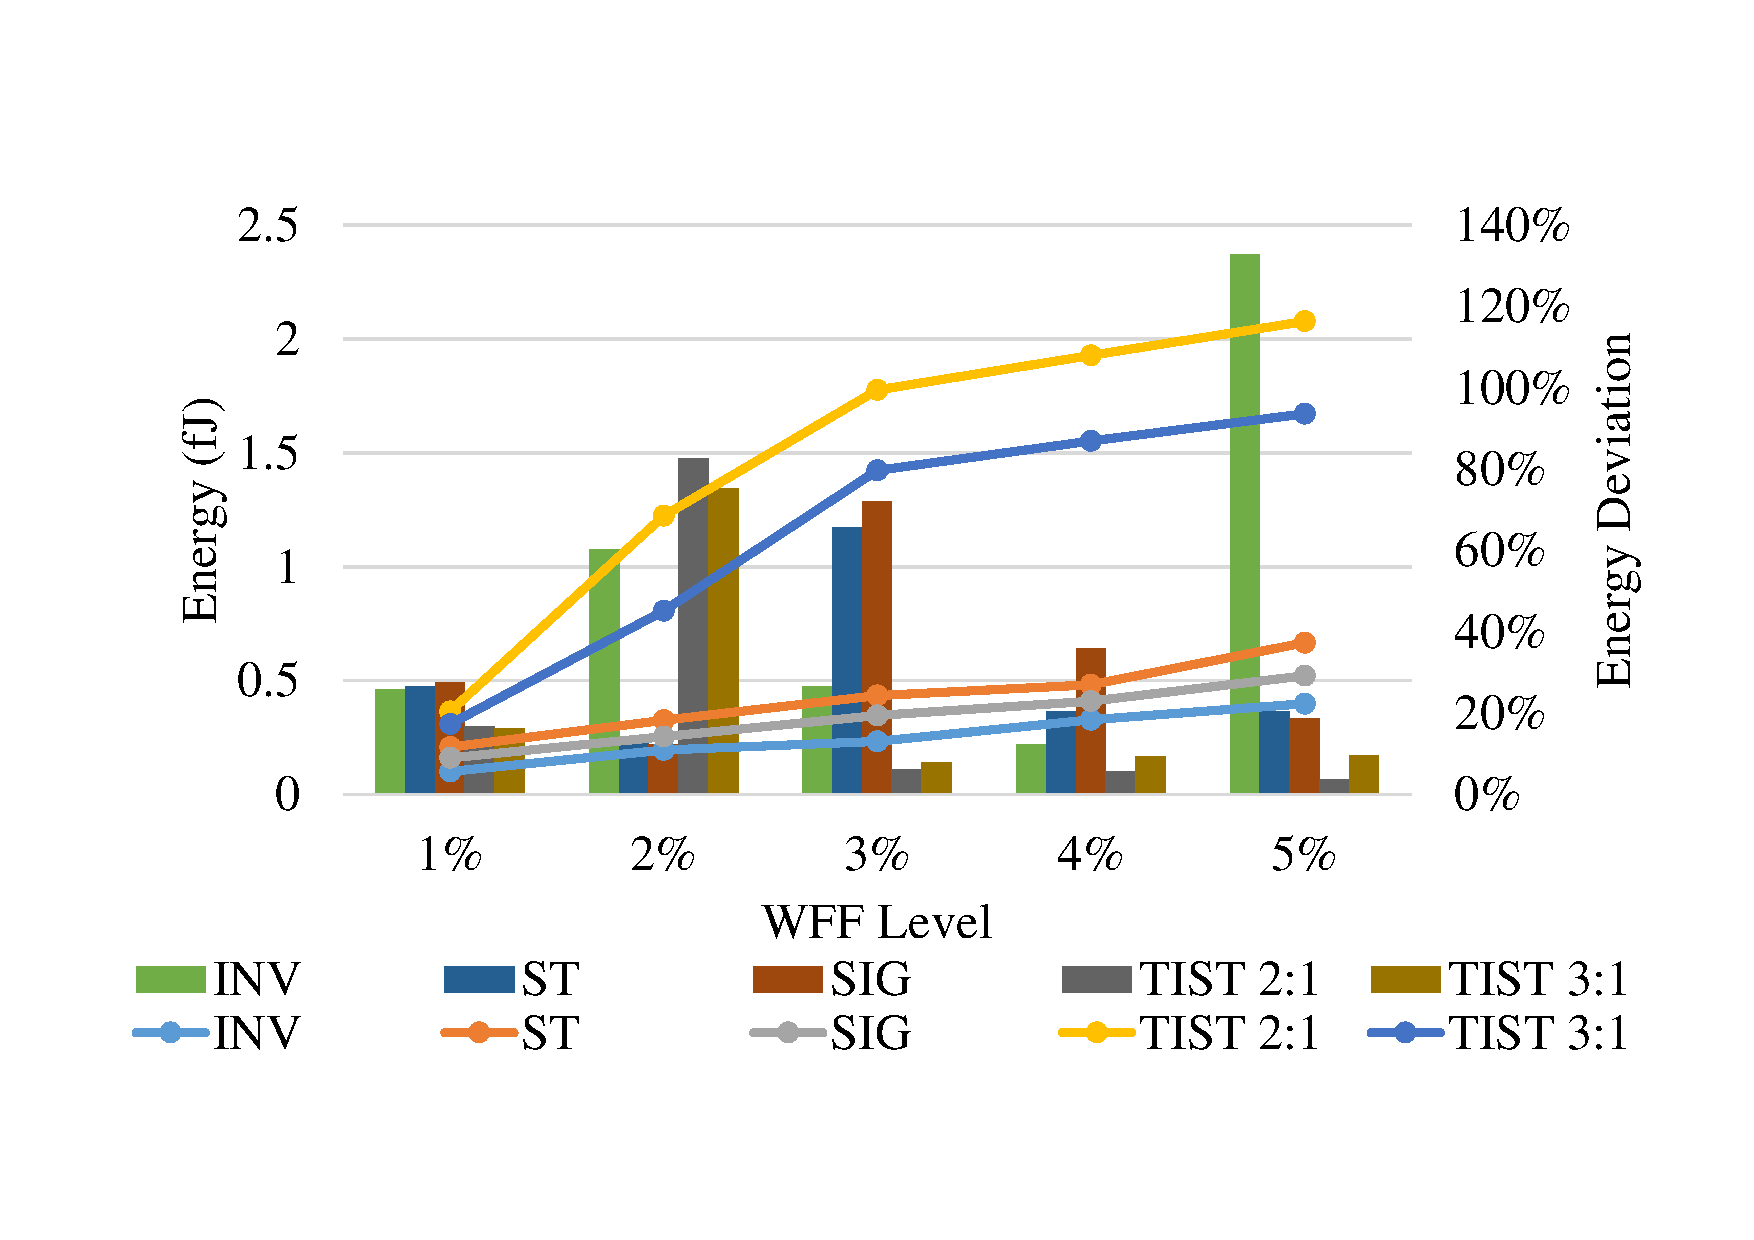
\includegraphics[width=0.9\textwidth, trim={1.25cm 3cm 2cm 3cm}, clip]{compLowEnergy.pdf}
            \caption{Low energy layouts energy metrics comparison for each design.}
        \label{figCompLowEnergy}
    \end{figure}

    For the high robustness spectrum, the energy consumption difference between designs follows the same behaviour, although with much broader differences. In comparison to the inverter energy consumption each design presented an average increase of 43.52\%, 263.24\%, 382.12\%, and 555.21\%, for the SIG, ST, TIST 3:1, and TIST 2:1, respectively. The deviation metrics presented a similar behaviour as well, although the ST presented the highest deviations. The TIST designs presented the lowest deviations with 3.56\%, and 5.55\% for the TIST 2:1, and 3:1, respectively. Following, the SIG, inverter, and ST, presented 6.23\%, 6.93\%, and 7.81\% deviations. In this case, the inverter is a strong candidate, with the lowest energy consumption, and acceptable robustness.

    \begin{figure}[]
        \centering
            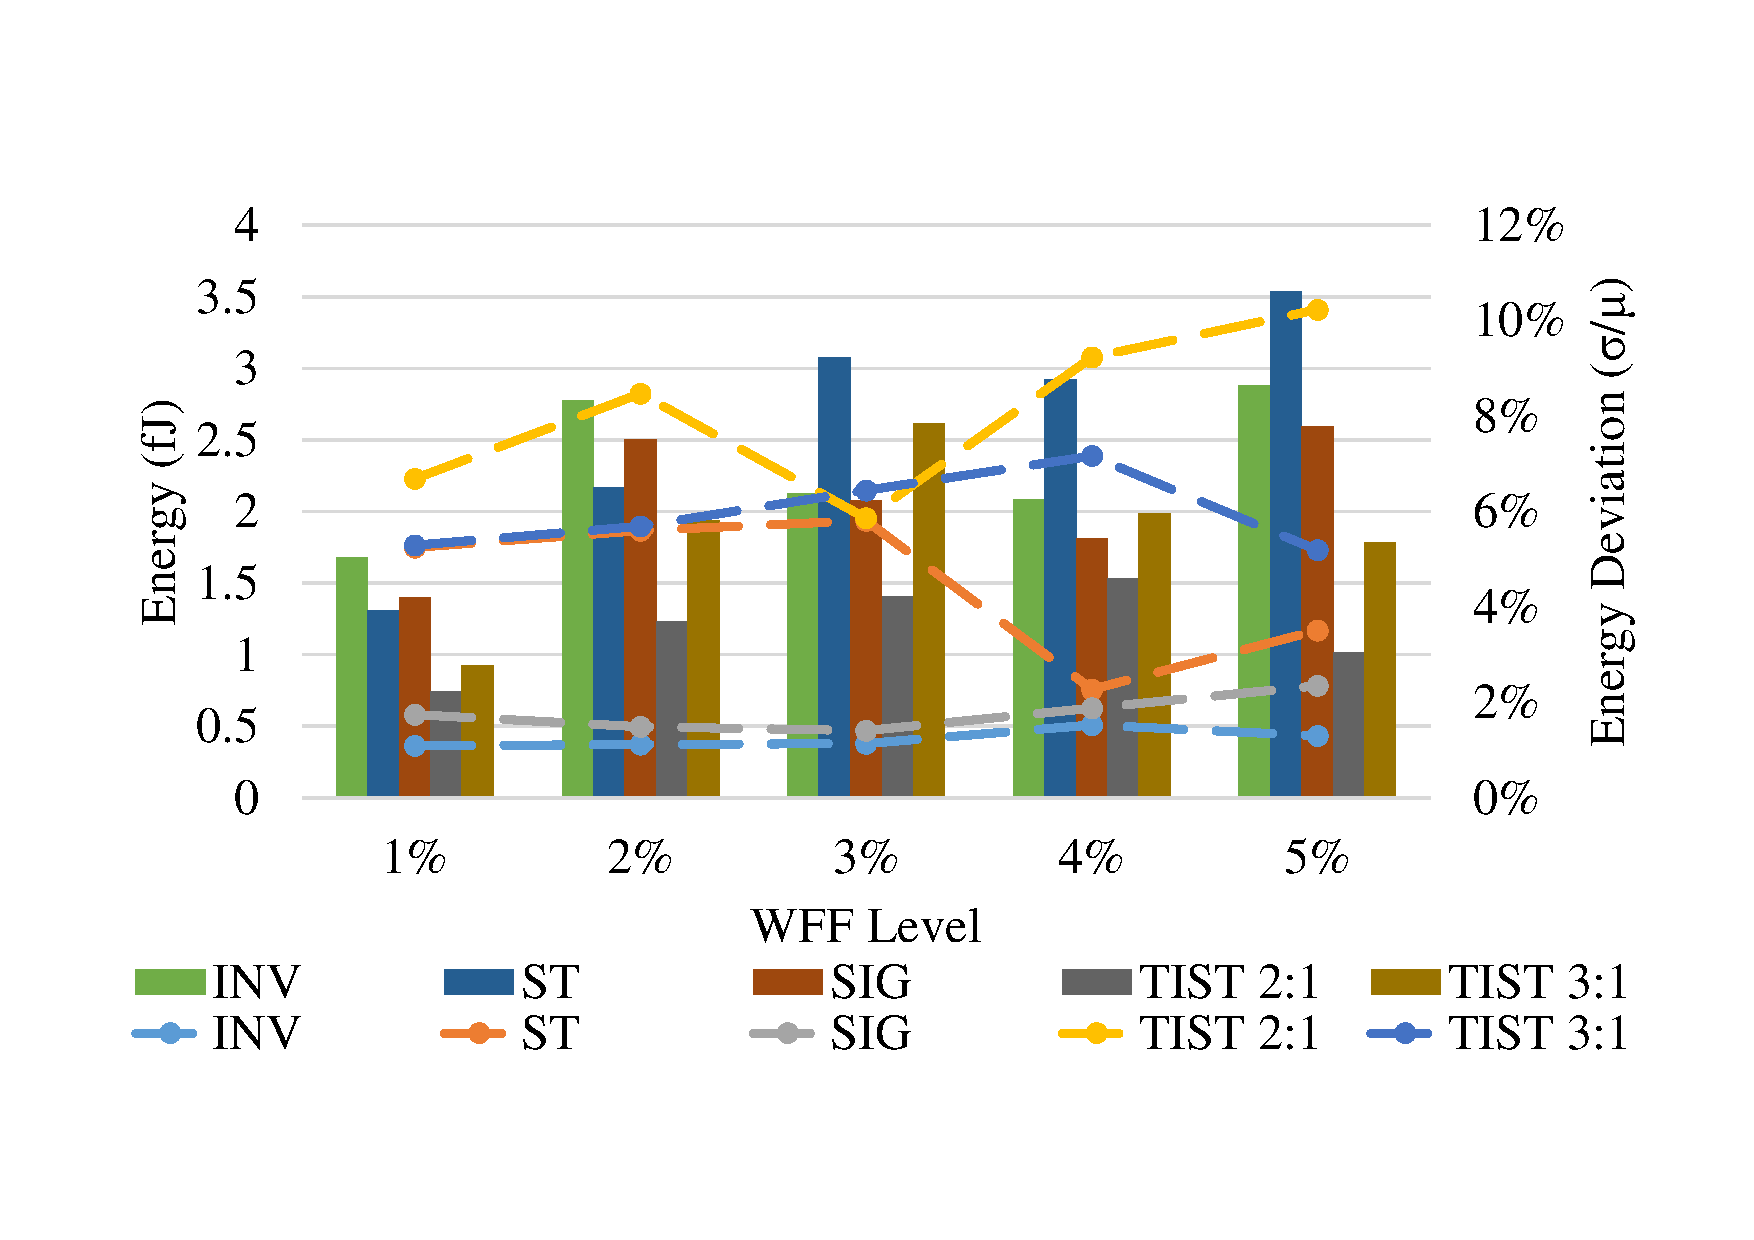
\includegraphics[width=0.9\textwidth, trim={1.25cm 3cm 2cm 3cm}, clip]{compHighRobustness.pdf}
            \caption{High robustness layouts energy metrics comparison for each design.}
        \label{figCompHighRobustness}
    \end{figure}

    Lastly, for the CB layouts, the energy consumption scaling through the designs is the same, although with smaller differences, even in comparison to the low energy layouts. In comparison to the inverter, the SIG, ST, TIST 3:1, and TIST 2:1 presented average increases of 18.84\%, 47.74\%, 281.85\%, and 379.6\%. The designs kept the same behaviour as their high robustness variants. The TIST designs presented the lowest deviations with 4.07\% and 5.8\% for the 2:1 and 3:1 proportions, respectively. The SIG, inverter and ST, presented respectively, 6.72\%, 7.05\%, and 8.74\% deviations on energy. In this case, the SIG, presents a higher energy consumption and much bigger layout, it only provides a minor improvement over deviations (4.91\%, relative to the inverter). The ST presented higher energy and bigger area as well, with a increase on deviations (1.69\%, absolute and 23.97\% relative increases, in comparison to the inverter), although it still presents hysteresis. The TIST designs, consume considerably more energy, with less deviation (although, as stated before, those numbers are deflated), bigger layout area, and less viable scenarios to work with.

    \begin{figure}[]
        \centering
            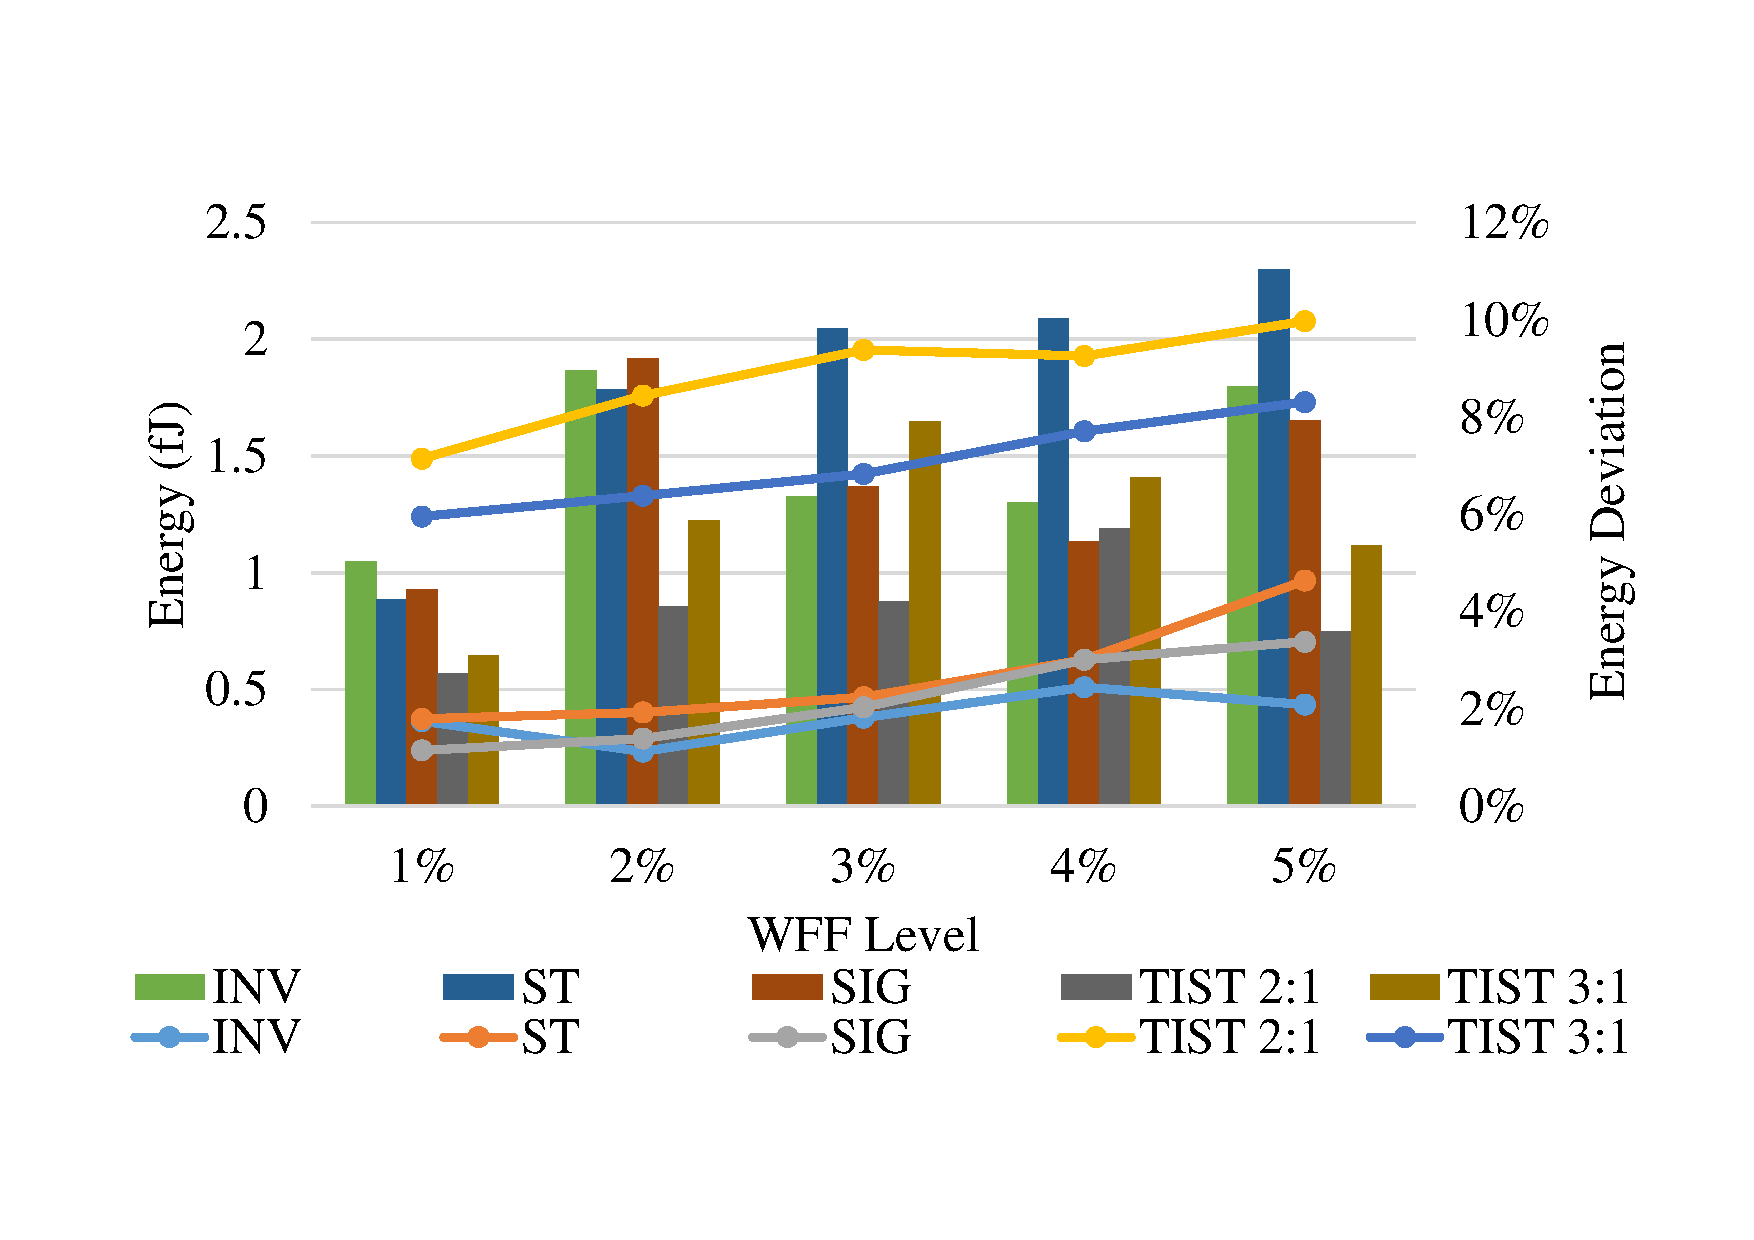
\includegraphics[width=0.9\textwidth, trim={1.25cm 3cm 2cm 3cm}, clip]{compCB.pdf}
            \caption{CB layouts energy metrics comparison for each design.}
        \label{figCompCB}
    \end{figure}

It is shown that the CB layouts presents similar energy deviations in comparison to the high robustness layouts while maintaining a lower energy consumption, for the ST and SIG, with the exception of the inverter. The inverter presents a high deviation for its minimum energy layout at 5\% WFF (1 fin layout with a supply voltage of 0.3V). Although, with a little increase on supply voltage, from 300mV to 400mV, matching the CB layout, the inverter presents a 8.95\% increase on energy consumption while decreasing its energy deviation by 93.49\%. The ST presented a similar results at 3\% WFF where a 100mV increase, from 200mV to 300mV of supply voltage, provided a reduction of 85.01\% in energy deviations while increasing the energy consumption by 7.86\%. For the SIG, at 3\% WFF as well, is was possible to decrease the deviation by 90.88\% while increasing the energy consumption by 22.09\%m, with the same supply voltage increase performed for the ST. Average and maximums differences in energy consumption and deviations between CB, low energy, and high robustness layouts are shown in Fig. \ref{CBCompLE} and Fig. \ref{CBCompHR}, respectively.

\begin{figure}[]
	\centering
       	\caption{Energy consumption and energy consumption deviations difference between the cost-benefit and low energy layouts. \label{CBCompLE}}        	  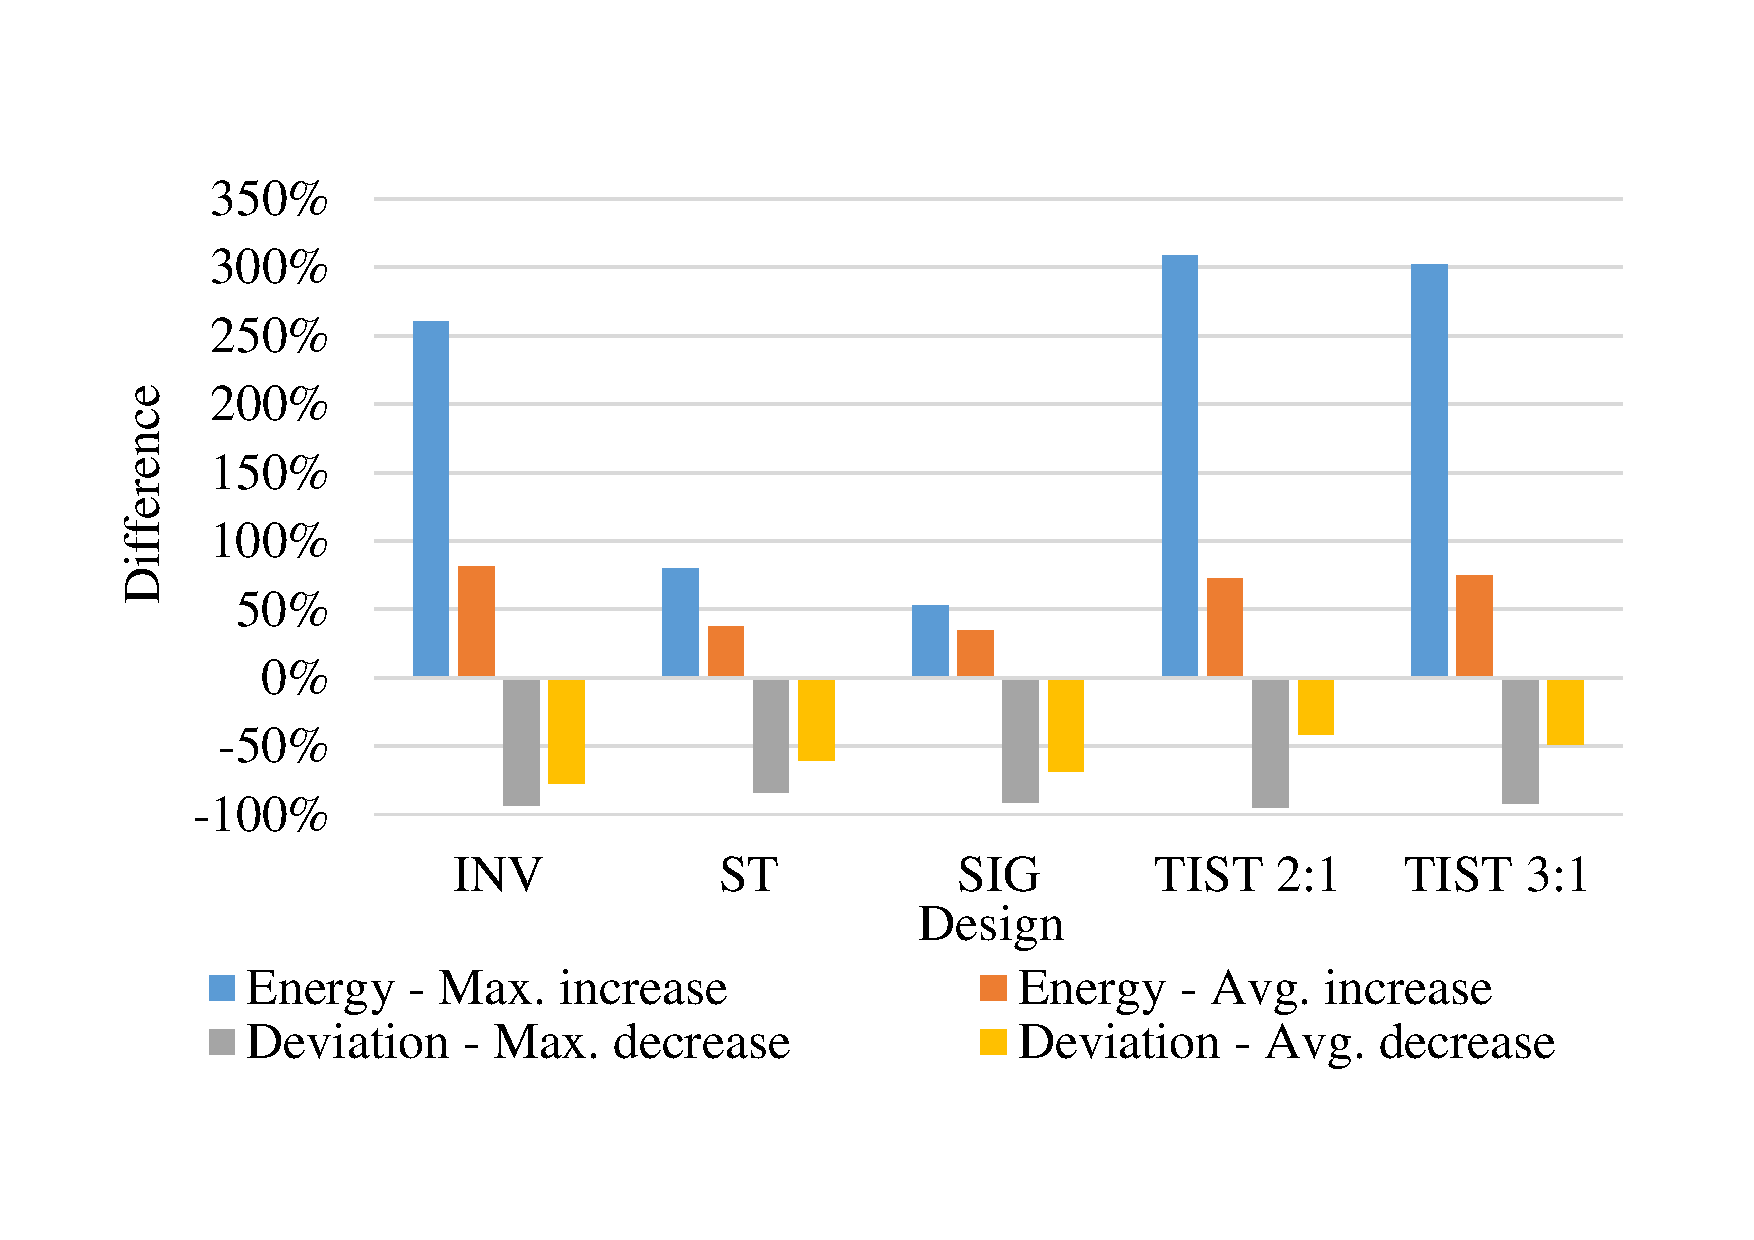
\includegraphics[width=0.9\textwidth, trim={1.25cm 2cm 2cm 3cm}, clip]{compCB-LE.pdf}
\end{figure}

\begin{figure}[]
	\centering
        \caption{Energy consumption and energy consumption deviations difference between the cost-benefit and high robustness layouts. \label{CBCompHR}}
      	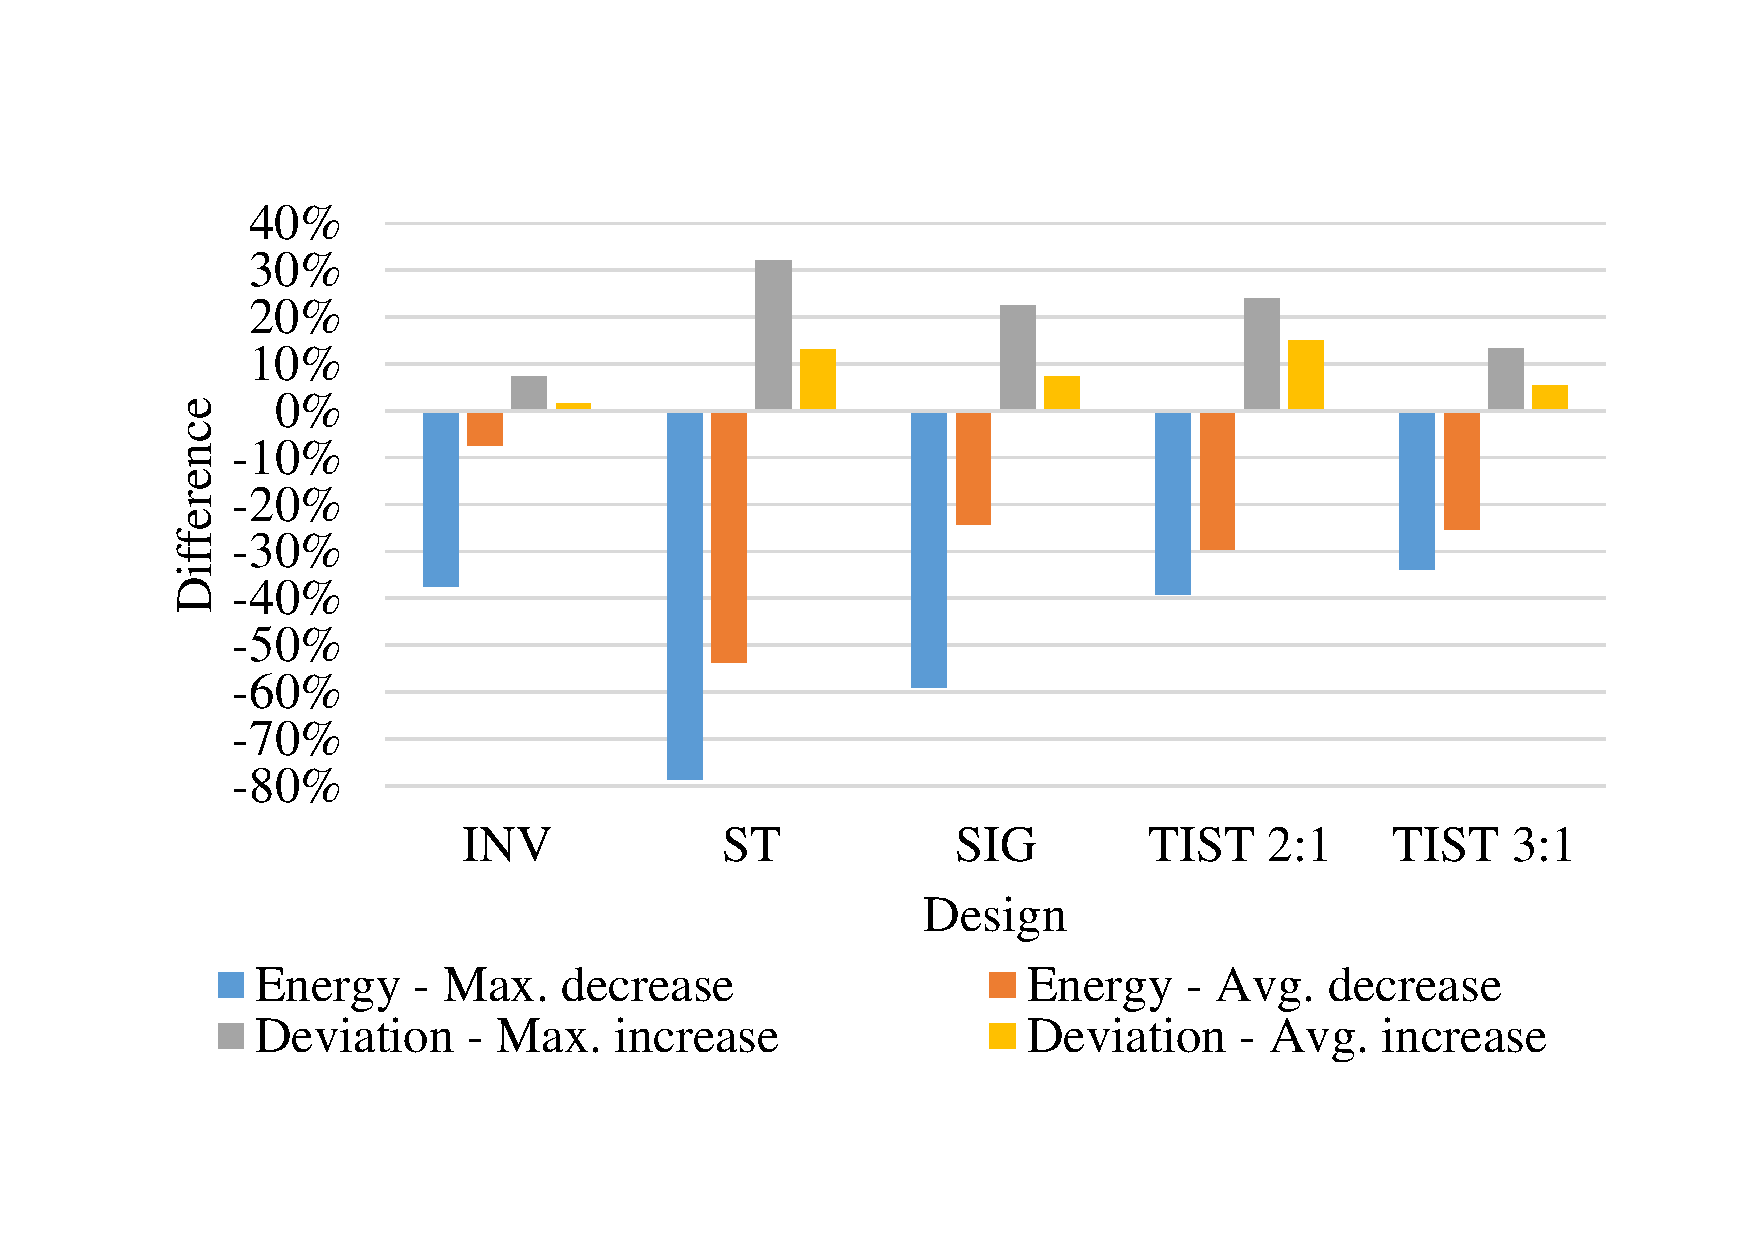
\includegraphics[width=0.9\textwidth, trim={1.25cm 2cm 2cm 3cm}, clip]{compCB-HR.pdf}
\end{figure}

    At the same time, it is important to analyze the drawbacks of a CB approach. The CB layouts for inverter and TIST layouts presented higher increases on energy consumption, in comparison to the ST and SIG designs. Higher average increase is directly related to the shift of a supply voltage from 100mV to 0.7V, at 1\% WFF. The supply voltage switch on the inverter is due to the considerable decrease in energy deviation (from 25.83\% to 5.04\%) of 5.125x, while the energy consumption increased 3.6x. For the TIST the higher energy increases are related to the lack of working scenarios at near-threshold, and the sudden increase in supply voltage, similar to the inverter. When observing the increases in energy deviations comparing the CB and high robustness layouts, the CB layouts can bring up to 32\% increase in energy deviations, although, causing an 79\% decrease in energy consumption, highlighting the differences between applications.

\section{Current Ratios}

%correntes
%	dinamica
%        	valores absolutos
%            		tensão de alimentação
%                		exponencial (maior a tensão, maior a corrente)
%            		nível de variabilidade
%				linear, praticamente nenhuma mudança
%		desvios
%			tensão de alimentação
%				exponencial decrescente (maior a tensão, menor o desvio)
%			nível de variabilidade
%				linear (maior a variabilidade, maior o desvio)
%    	estática
%		valores absolutos
%        		tensão de alimentação
%				linear (maior a tensão, maior a corrente)
%			nível de variabilidade
%				exponencial (maior a variabilidade, maior a corrente)
%		desvios
%			tensão de alimentação
%				linear, praticamente uma reta
%			nível de variabilidade
%				exponencial amortecida



    When considering the impact of process variability into the energy consumption, it will depend of the propagation times and the power consumption, and their respective deviations. Performance and power are highly dependent on the value and stability of the devices currents, either dynamic (on) and static (off). The devices delays are highly dependent on how fast can the circuit switch its value, which is related to the circuit parasitics and its dynamic current. In parallel, the circuit power, being a function of the current and resistances will suffer higher influence from current values and deviations. In order for the circuit to maintain its signals well defined, fast signal value switching, and low static power consumption, it is recommended to maintain the on and off current high and low as possible, respectively. The ideal current setup may be achieved through circuit level methods or the apropriate transistor sizing, where the length and width of the channel will be fine tuned in order to achieve the highest ratio possible between currents.

In order to more clearly understand the impact of process variability and supply voltage influence on current behaviour, the dynamic and static currents average measures and normalized standard deviations will be explored. The graphs are divided in two parts for each current, with average measures and normalized standard deviations. Fig. \ref{fig:dynCurrAbs} and Fig. \ref{fig:dynCurrDev} present the average values and normalized standard deviations for the dynamic current. It can be observed an exponential and an overall linear dependency over supply voltage and WFF level, respectively, with the current slightly decreasing due to WFF level. Although, when considering sub-200mV supply voltages, the average dynamic current will increase exponentially as variability level scales. This happens due to the higher number of extreme cases where the worst-case measure can be up to 5-orders of magnitude higher than the average. For the normalized standard deviations of the dynamic current, there are exponential dependencies over both variables when considering low supply voltage/high variability level scenarios, with curves presenting a linear behaviour at the remaining scenarios.
%dificil trabalhar nessa tensão então por causa da corrente



    \begin{figure}[t]
        \centering
            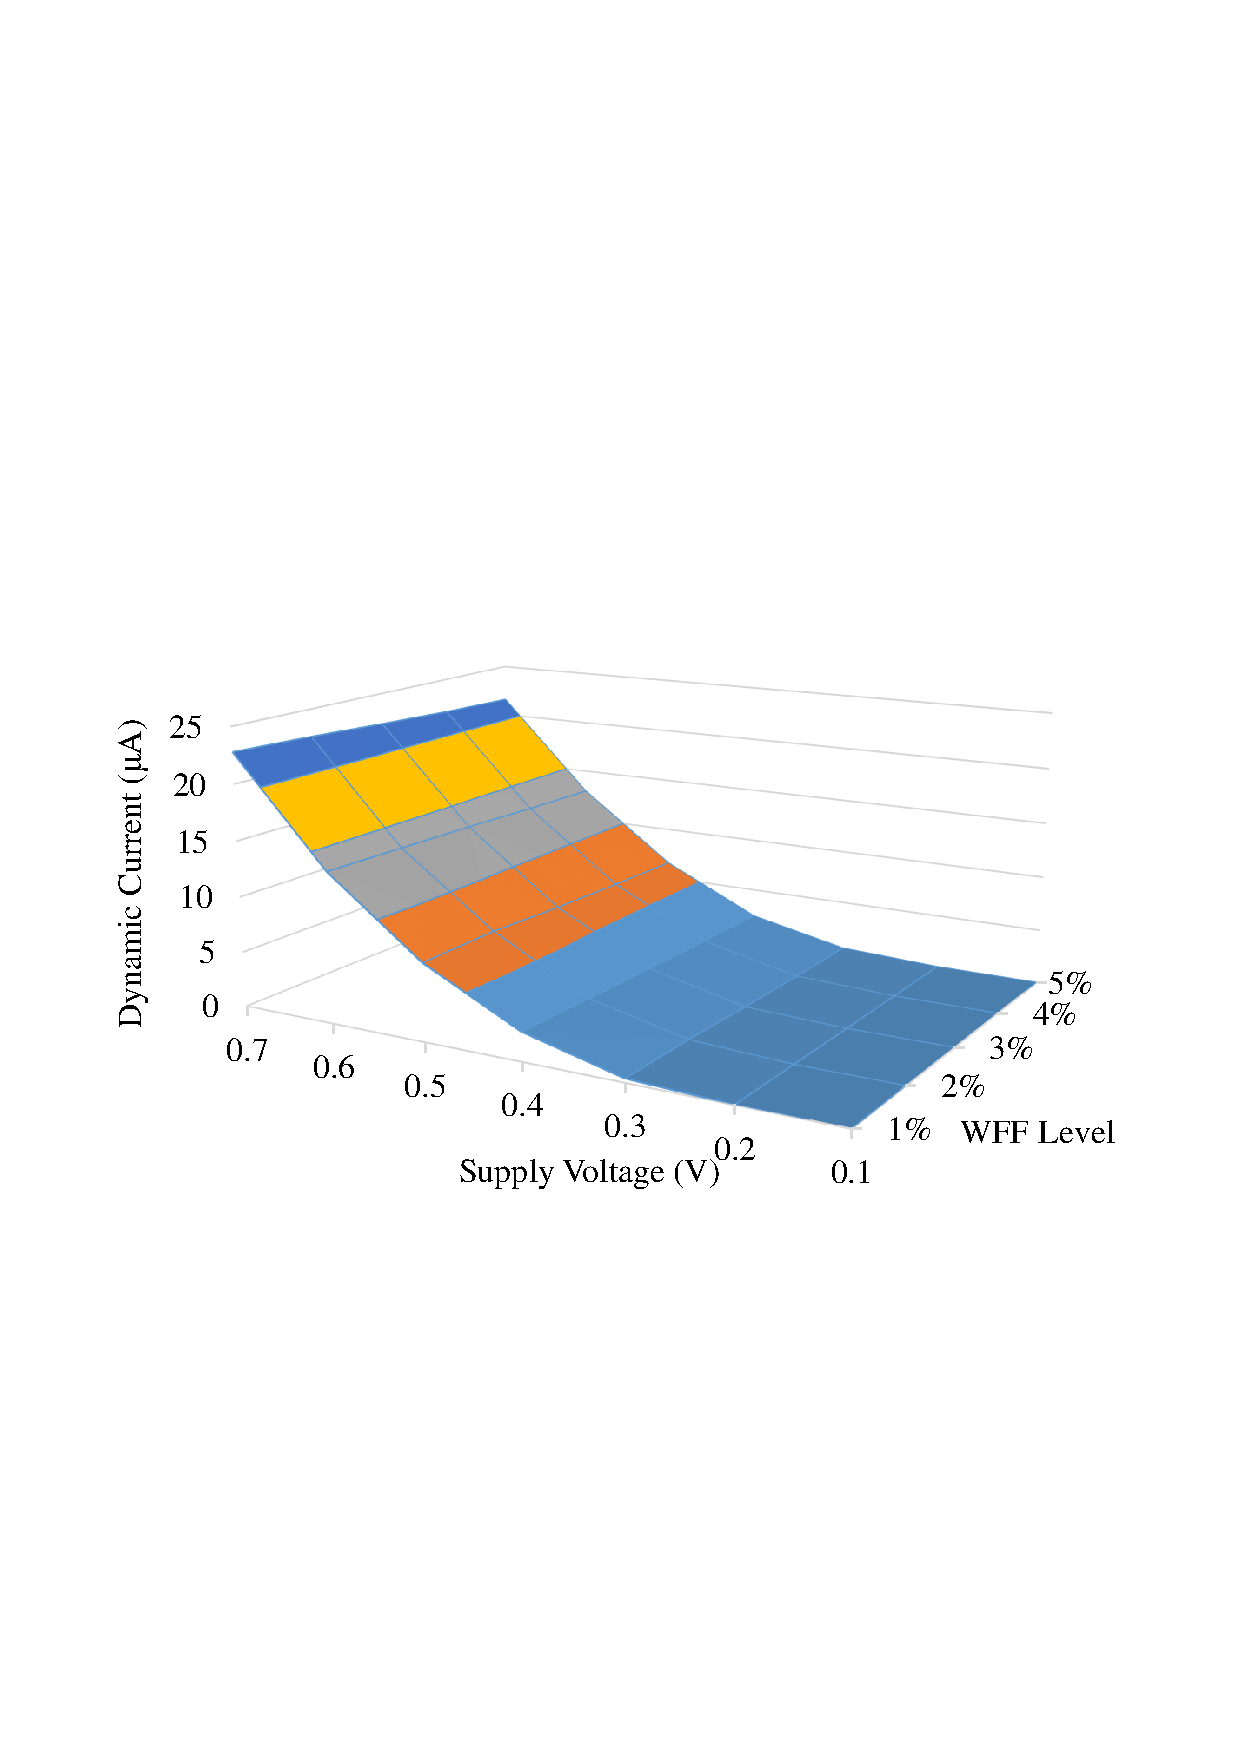
\includegraphics[width=0.85\textwidth, trim={1.25cm 9cm 2cm 11cm}, clip]{dynamicCurrAbs.pdf}
            \caption{Dynamic (on) current average measures through supply voltage and WFF scaling.}
        \label{fig:dynCurrAbs}
    \end{figure}

    \begin{figure}[]
        \centering
            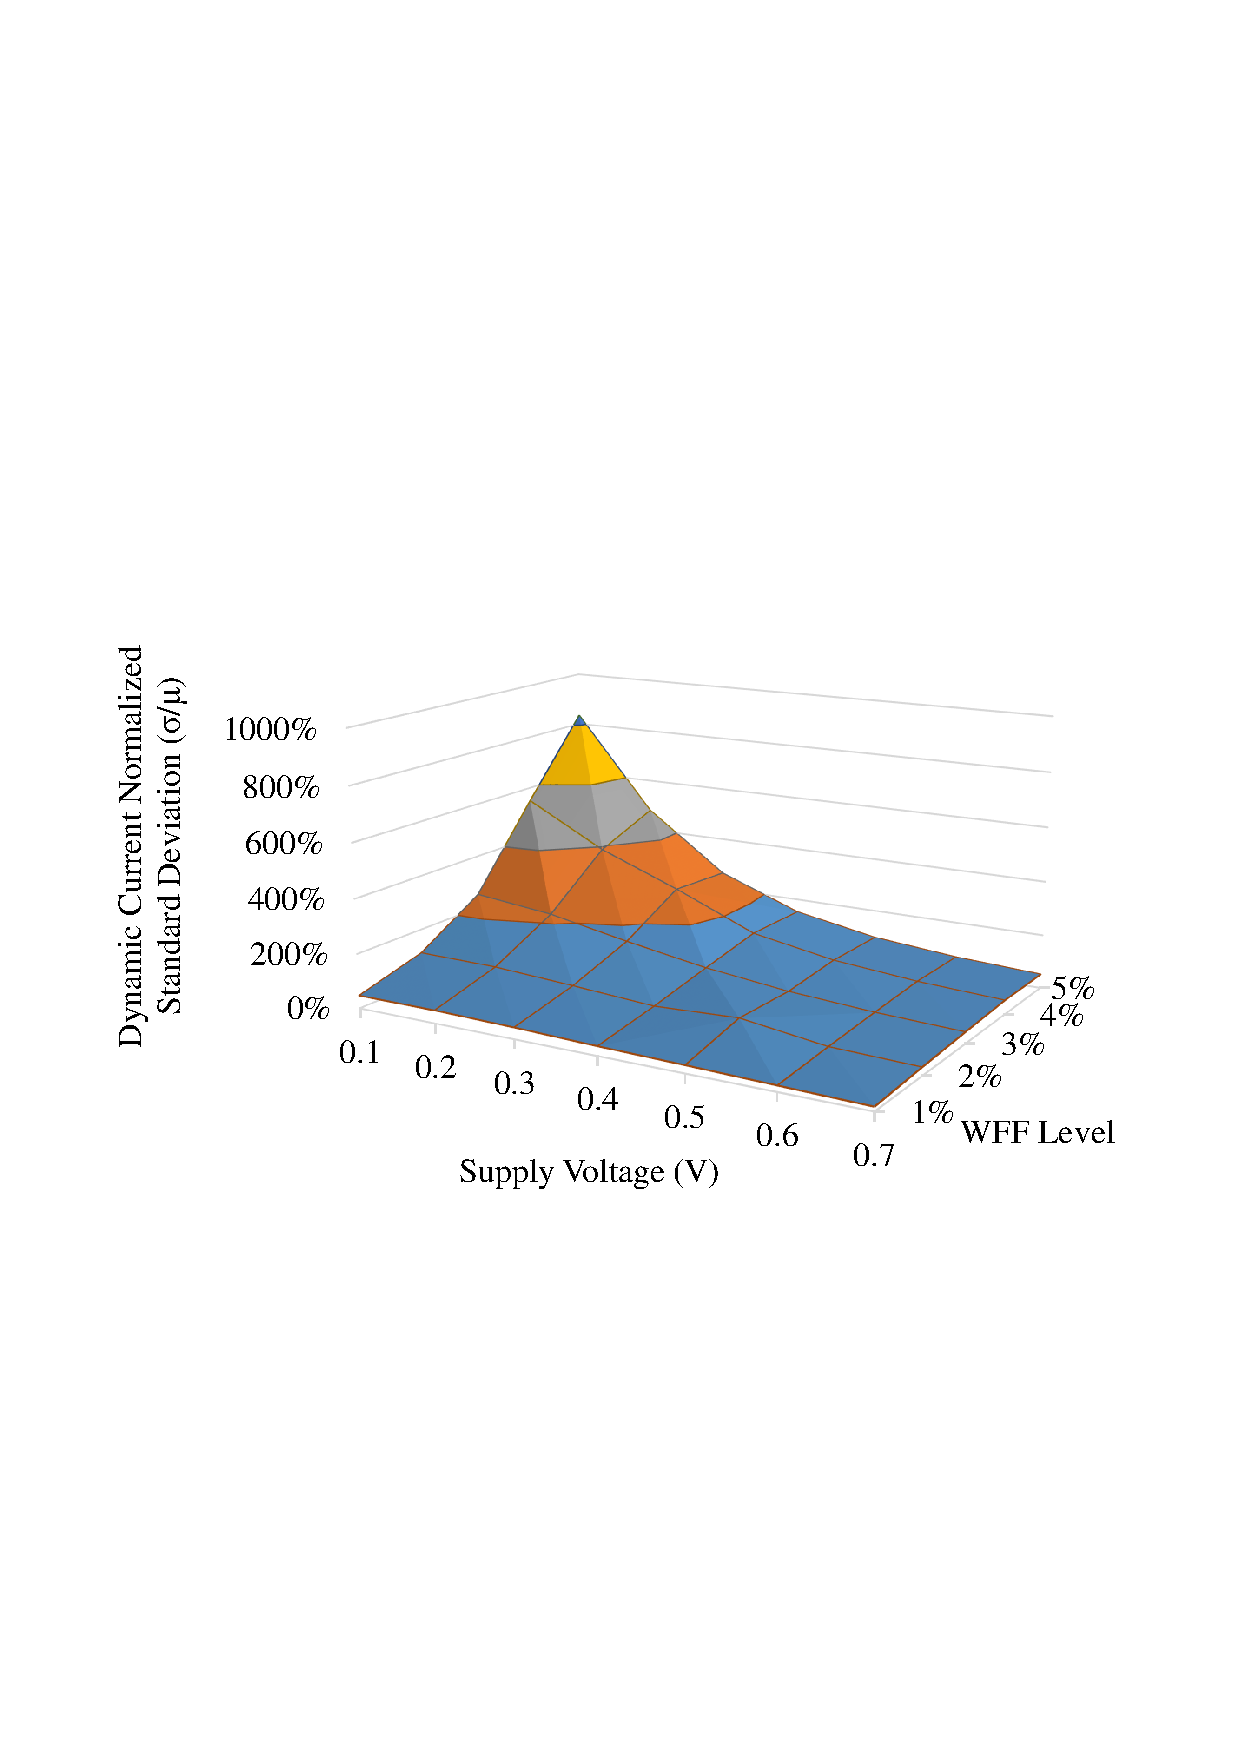
\includegraphics[width=0.85\textwidth, trim={1.25cm 9cm 2cm 10.5cm}, clip]{dynamicCurrDev.pdf}
            \caption{Dynamic (on) current normalized standard deviations through supply voltage and WFF scaling.}
        \label{fig:dynCurrDev}
    \end{figure}

Fig. \ref{fig:StatCurrAbs} and Fig. \ref{fig:StatCurrDev} present the results for the static current. The average measures will exponentially scale due to the process variability level and linearly decrease as the supply voltage scales down. The normalized standard deviations for the static current presents a linear relation with the supply voltage, with a 16\% difference between the lowest and highest average normalized deviations, and a exponential dependency over variability level, with averages doubling at each WFF level increase step.


    \begin{figure}[t]
        \centering
            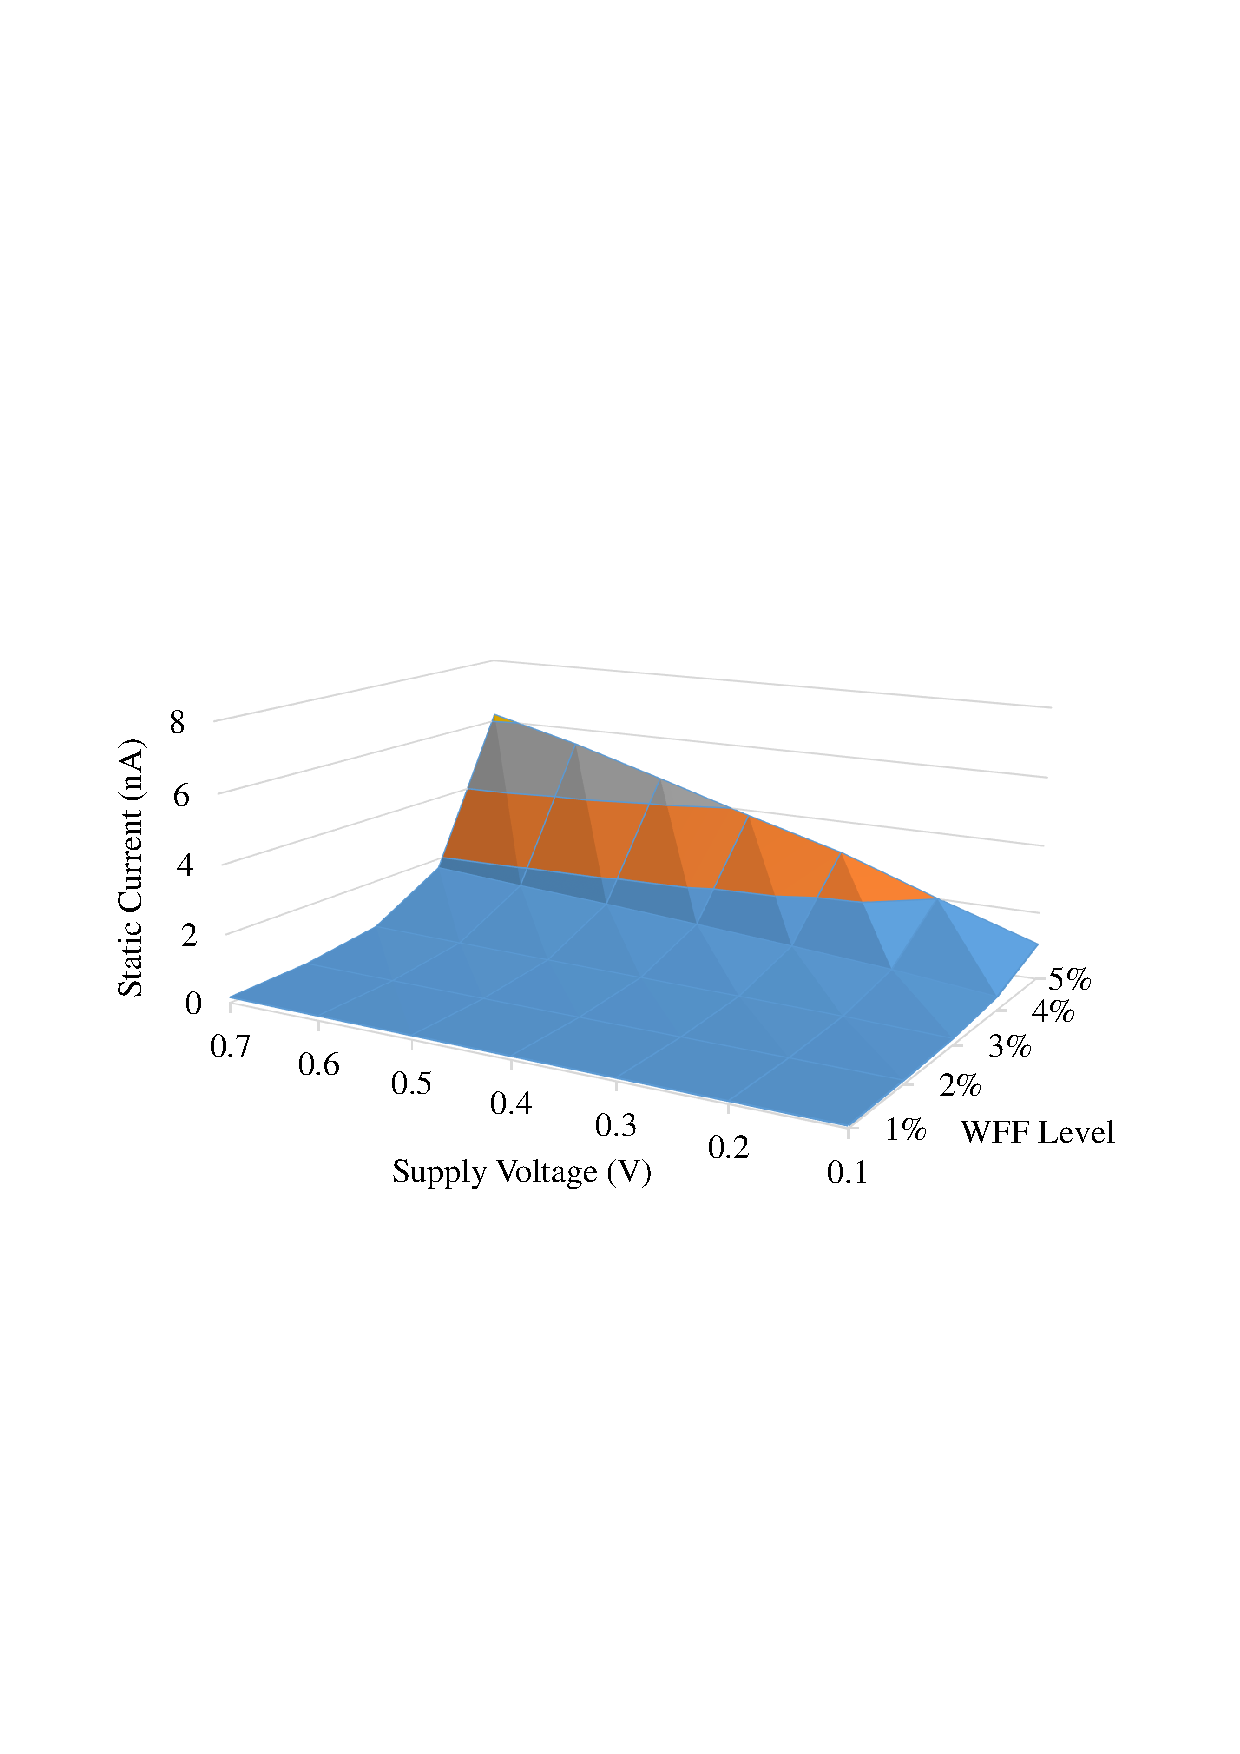
\includegraphics[width=0.85\textwidth, trim={1.25cm 9cm 2cm 11cm}, clip]{staticCurrAbs.pdf}
            \caption{Static (off) current average measures through supply voltage and WFF scaling.}
        \label{fig:StatCurrAbs}
    \end{figure}

    \begin{figure}[h]
        \centering
            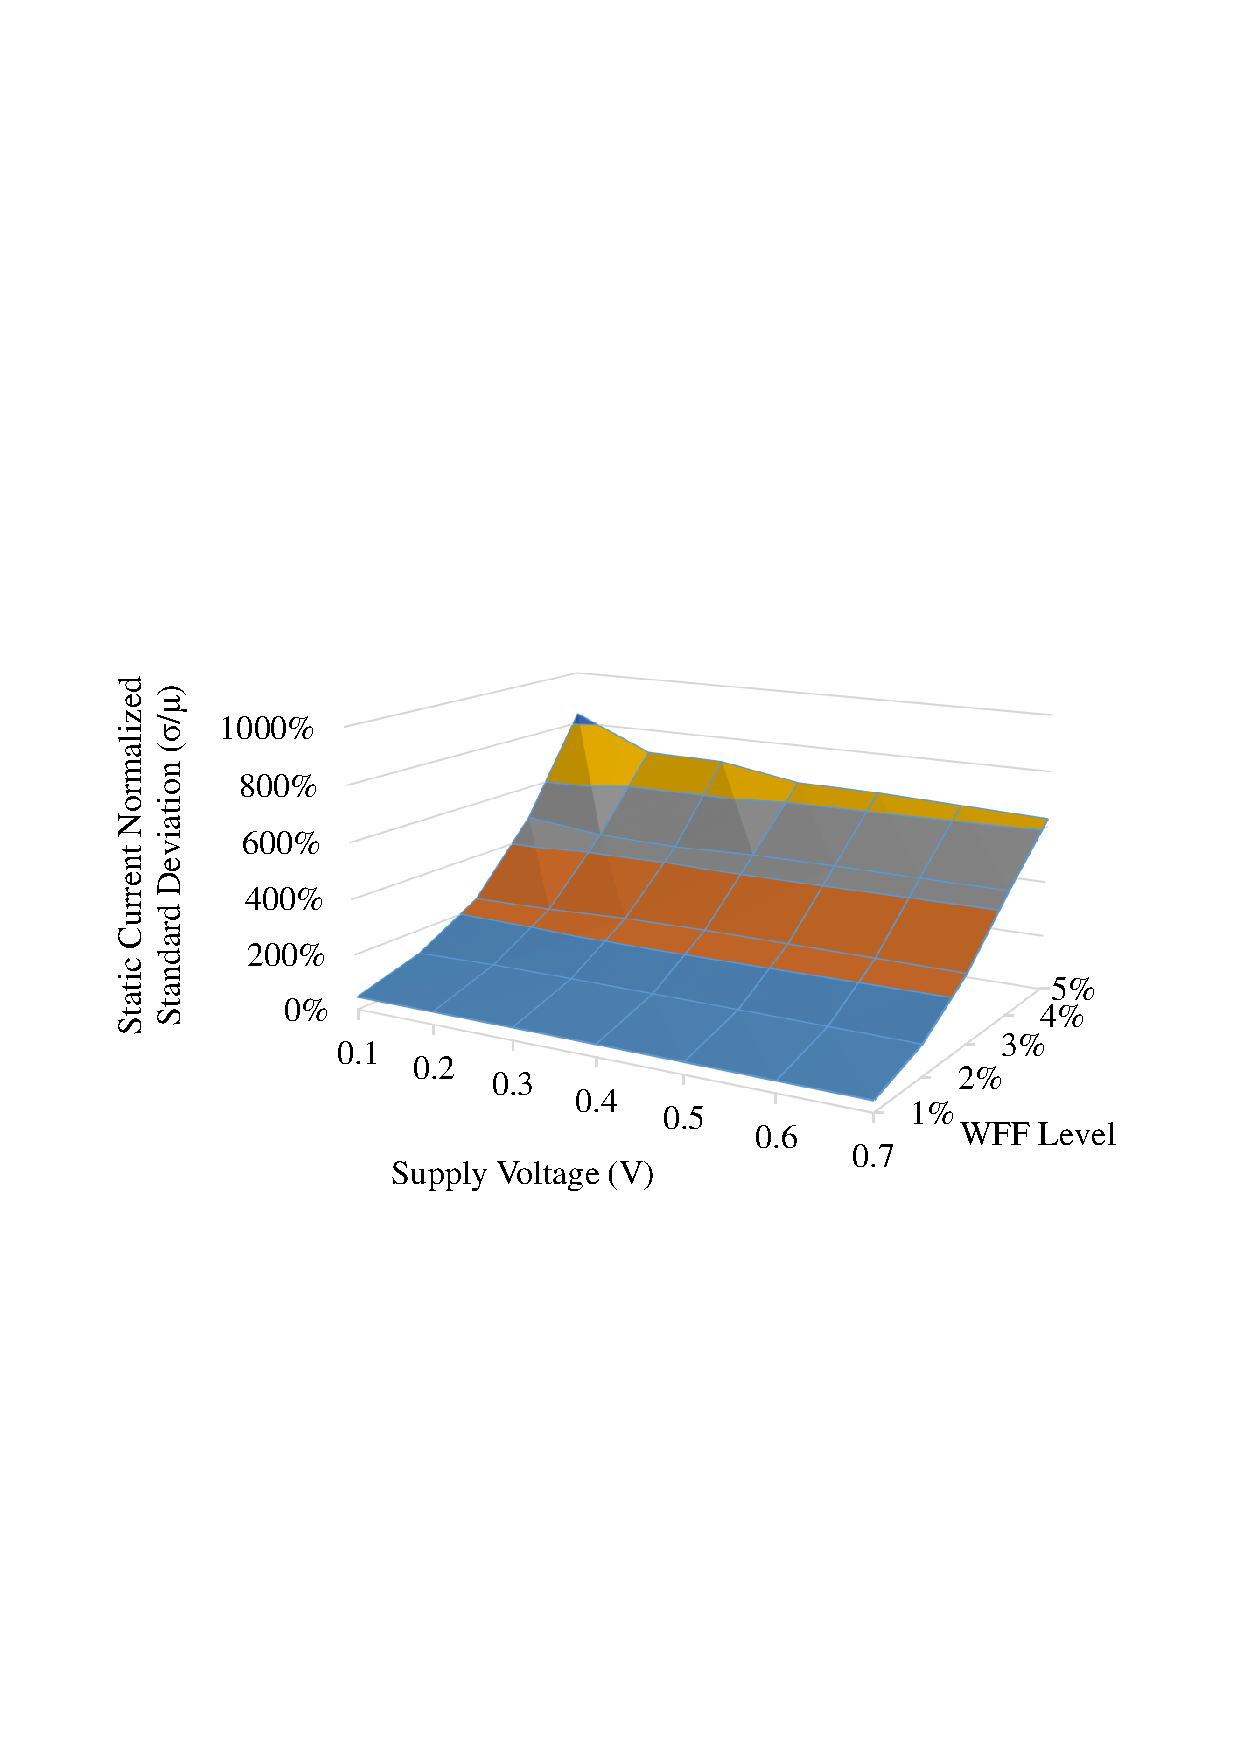
\includegraphics[width=0.85\textwidth, trim={1.25cm 9cm 2cm 11cm}, clip]{staticCurrDev.pdf}
            \caption{Static (off) current normalized standard deviations through supply voltage and WFF scaling.}
        \label{fig:StatCurrDev}
    \end{figure}



As shown in Fig. \ref{figOnOffScal}. due to the linear and exponential dependency of the dynamic and static current measures upon the variability level, the static current presents a much higher scaling factor, in comparison to its counterpart. Given so, the current ratios will present a decrease as the process variability level increases, as shown in Fig. \ref{figsCurrComp}. Comparing to the inverter, the ST, TIST 2:1, and TIST 3:1 presented, on average, 118.01\%, 600.21\%, and 468.7\% higher ratios. The SIG is the only design which presented a worsening, with a 12.53\% lower ratio. While considering deviations into the ratio due to process variability, the ST and SIG presented 11.1\% and 6.91\% lower deviations, with the TIST 2:1 and 3:1 presenting 49.57\% and 42.79\% higher deviations, respectively.

    \begin{figure}[h]
        \centering
            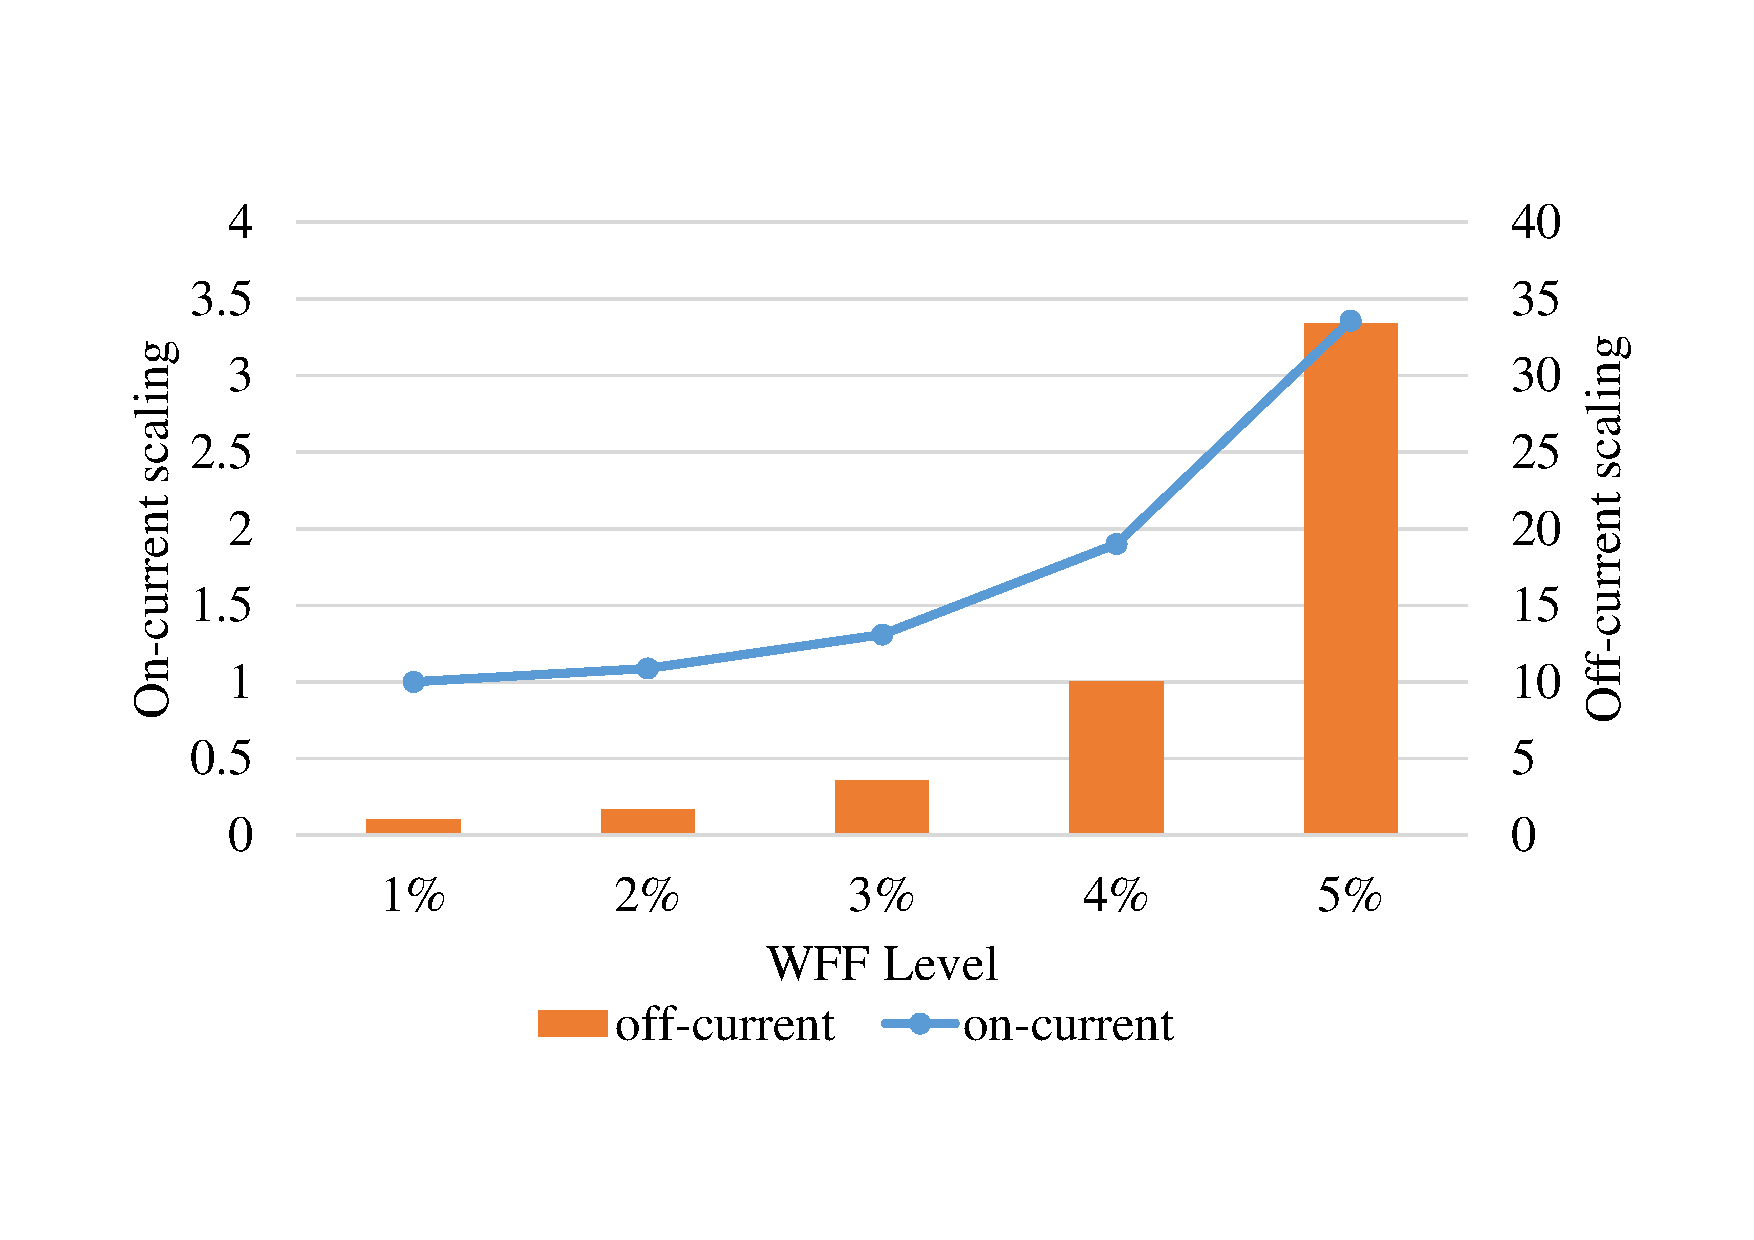
\includegraphics[width=0.85\textwidth, trim={1.25cm 3cm 2cm 3cm}, clip]{on-off-scaling2.pdf}
            \caption{Average on and off-current increase over all designs through variability scaling. The scaling is normalized in relation to the 1\% WFF level measures.}
        \label{figOnOffScal}
    \end{figure}

    \begin{figure}[H]
        \centering
            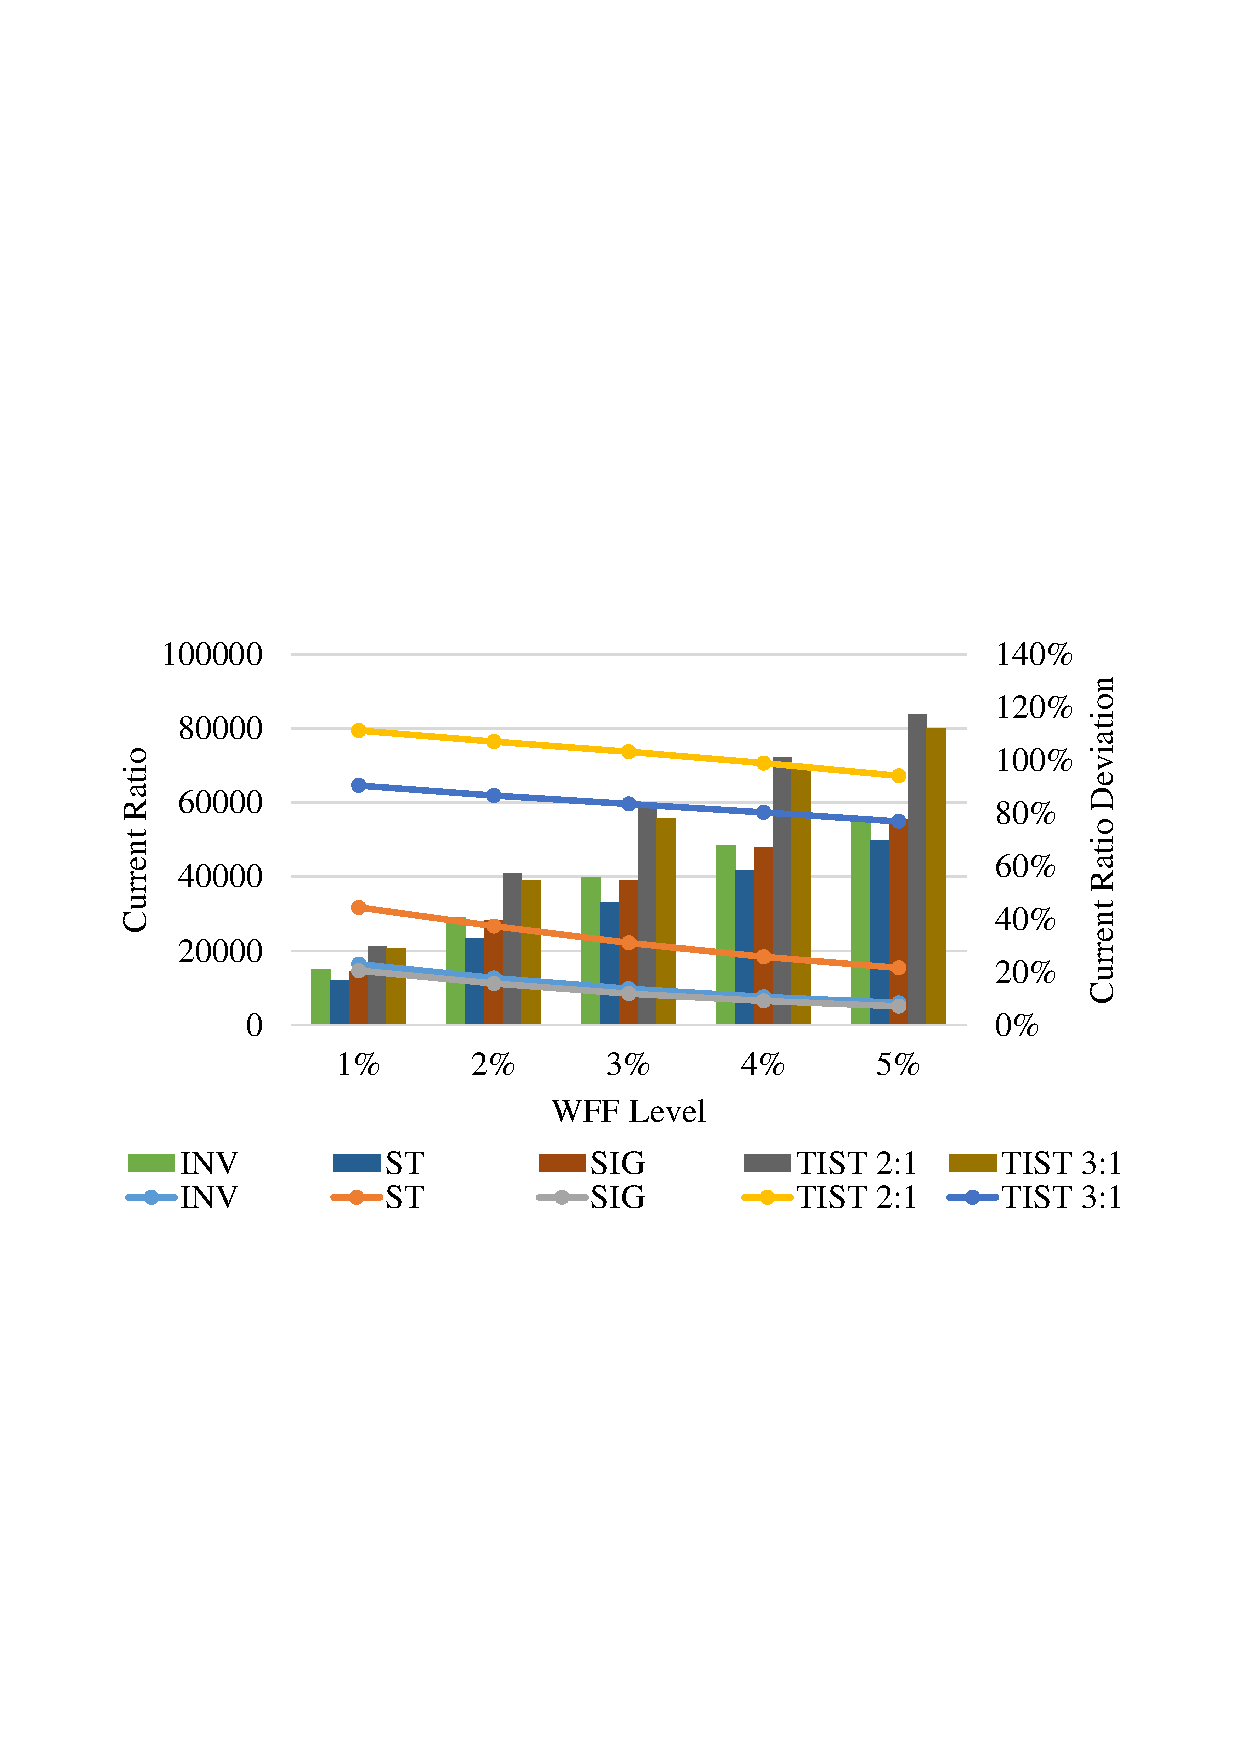
\includegraphics[width=0.85\textwidth, trim={1.25cm 9cm 2cm 10cm}, clip]{currRatioWFF.pdf}
            \caption{Current ratio (left) and current ratio deviation (right) design comparison across variability scaling.}
        \label{figsCurrComp}
    \end{figure}

When considering the ratio decrease, the TIST designs presented the lowest decrease, at 15.21\%, with the ST, inverter, and SIG presenting much higher losses with 51.44\%, 63.59\%, 65.54\%, respectively. In more depth, as shown in Fig. \ref{fig:OnOffDev}, in comparison to the inverter, for the on-current, the ST, TIST 2:1, and TIST 3:1 presented 33.63\%, 44.45\%, and 43.23\% lower normalized deviations, respectively. Meanwhile, for the off-current, the improvements were narrower with a 6.27\%, 4.89\%, and 4.37\% lower off-current normalized deviations for the ST, TIST 2:1 and, TIST 3:1, respectively. The SIG presented little to no improvement, staying below 1\% decrease on both deviations. For the off-current measures, in comparison to the inverter, the SIG and ST presented 101.03\% and 155.69\% higher currents, while the TIST 2:1 and 3:1 designs, presented 339.61\% and 438.11\% increases.

    \begin{figure}[]
        \centering
            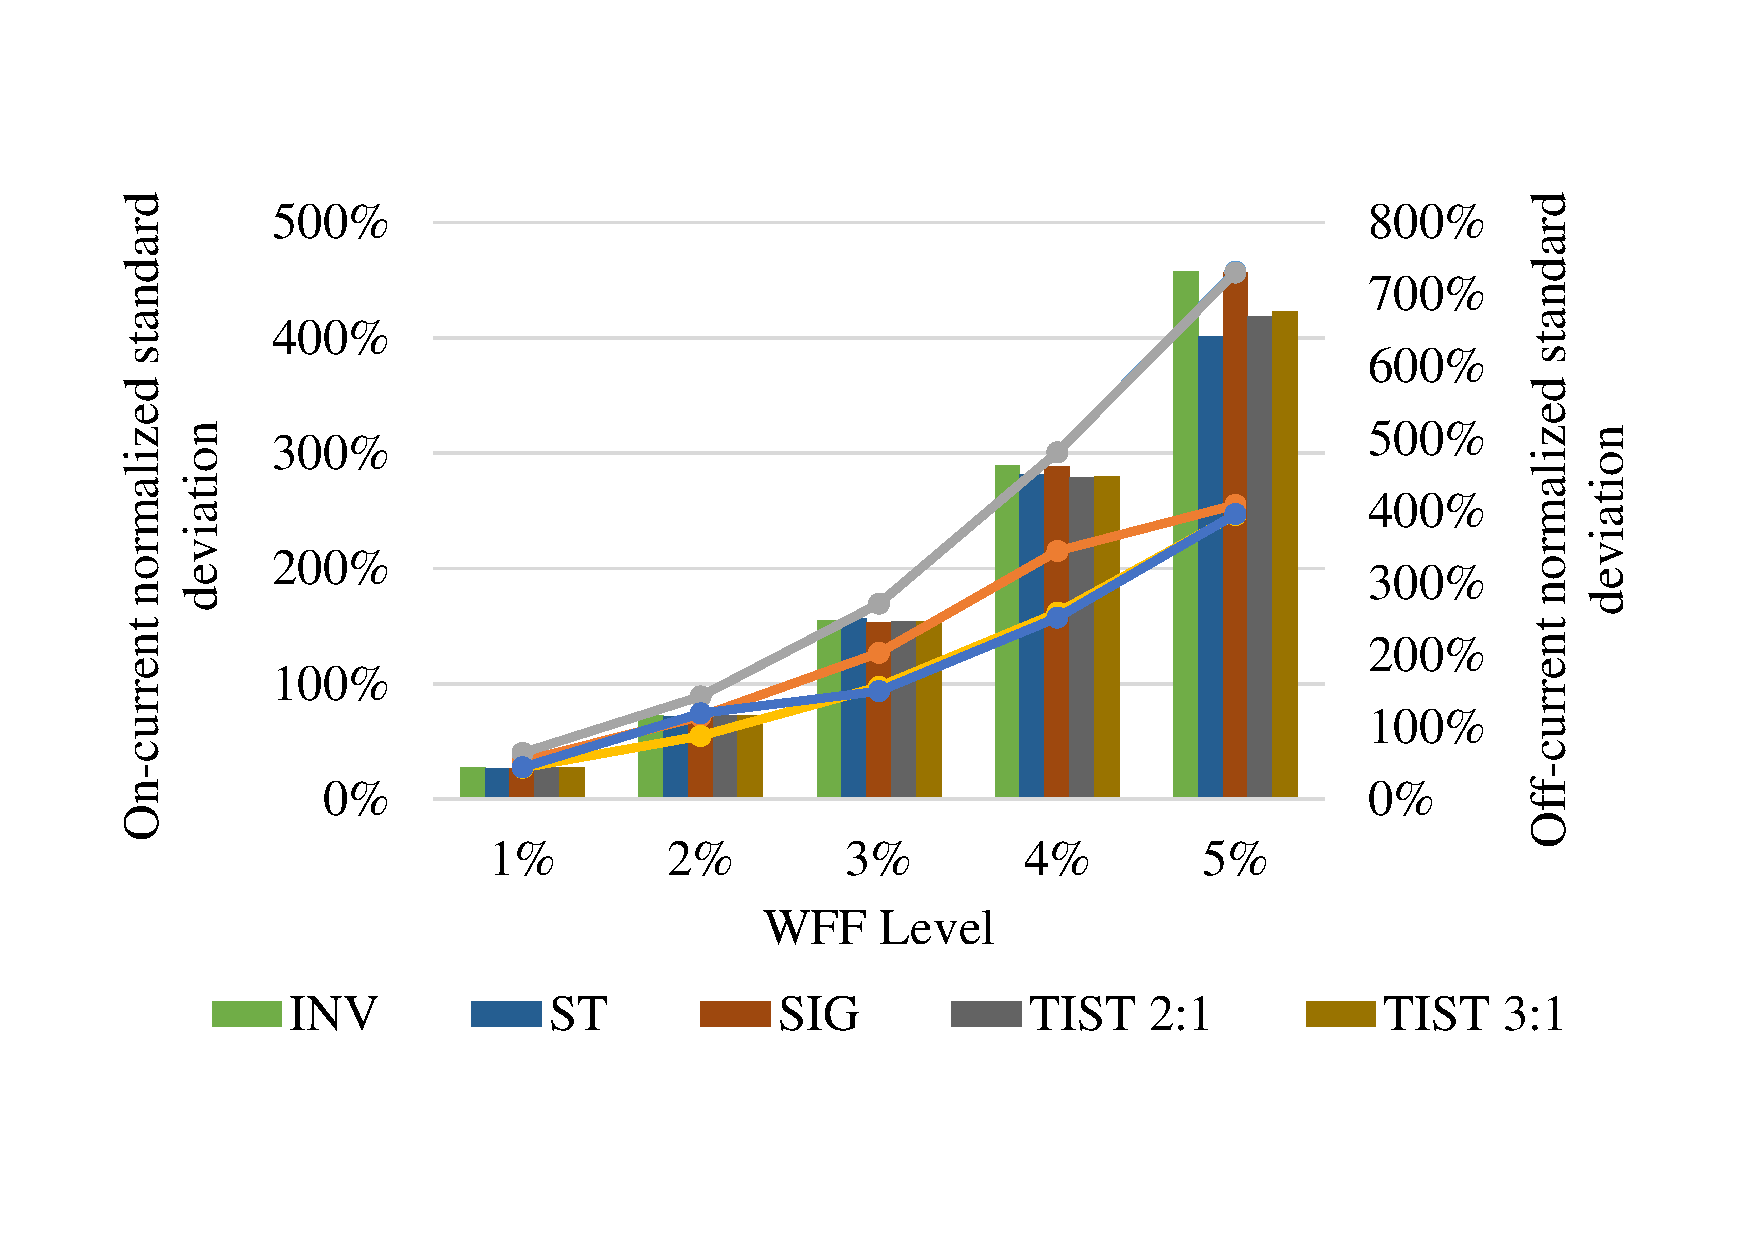
\includegraphics[width=0.9\textwidth, trim={1.25cm 1cm 2cm 3cm}, clip]{compOnOffCurr.pdf}
            \caption{Average on and off-current normalized deviation over all designs through variability scaling. The marked line is related to the on-current normalized deviations (left axis) while the bars are related to the off-curent normalized deviation (right axis).}
        \label{fig:OnOffDev}
    \end{figure}


Given all the current-related results, the TIST designs present the lowest deviations for the dynamic current, lowest ratio loss and highest current ratio. The ST showed the lowest deviations for the static current and lowest ratio deviations.




%Given so, when comparing inverter circuits, intended for decreasing the process variability impact upon metrics, it is important to achieve the highest current ratio possible. When concerning the $I_{on}$/$I_{off}$ ratios,



    %Due to the variability impact, the current ratios tend to decrease. This mainly happens due to the increase of the off-current as variability scales. This behavior is due to the effects of DIBL (Drain-Induced Barrier Lowering) and is a consequence of the short channel present on modern transistors. Due to the decreasing channel length, the depletion regions of drain and source become an increasing fraction of the whole area under the gate. Therefore, the volume of the depletion region effectively controlled by the gate decreases which can be modeled by a threshold voltage decreasing with the gate length. The charge below the gate being not only controlled by the gate but also by the drain and source regions is called the charge sharing effect. A similar effect occurs if the drain potential of the transistor increases: the pn-junction between the drain and the substrate becomes more reverse-biased, so the depletion layer grows and reduces even more the volume controlled by the gate. Given so, a drain bias-dependent threshold voltage can be assumed, as shown in Equation \ref{eqn:DIBL} \cite{henzler2006power}:

     % \begin{equation}
     %   \centering
     %   \label{eqn:DIBL}
     %   V_{th} = V_{th,0} - mV_{DS}
     %\end{equation}

    %Thus, according to Equation \ref{eqn:sub} \cite{henzler2006power}, where $I_{D,sub}$ is the subthreshold current (leakage current), the leakage current is exponentially dependent on the threshold voltage, as shown in Fig. \ref{figsOffCurrComp} for the inverter, although all designs presented the same behavior.
    %\begin{equation}
    %    \centering
    %    \label{eqn:sub}
    %    I_{D,sub} = I_0 \cdot exp\left(\frac{V_{GS} - V_{th,0} + mV_{DS}}{\eta \cdot V_T}\right)
    %\end{equation}

    %\begin{figure}[]
    %    \centering
    %        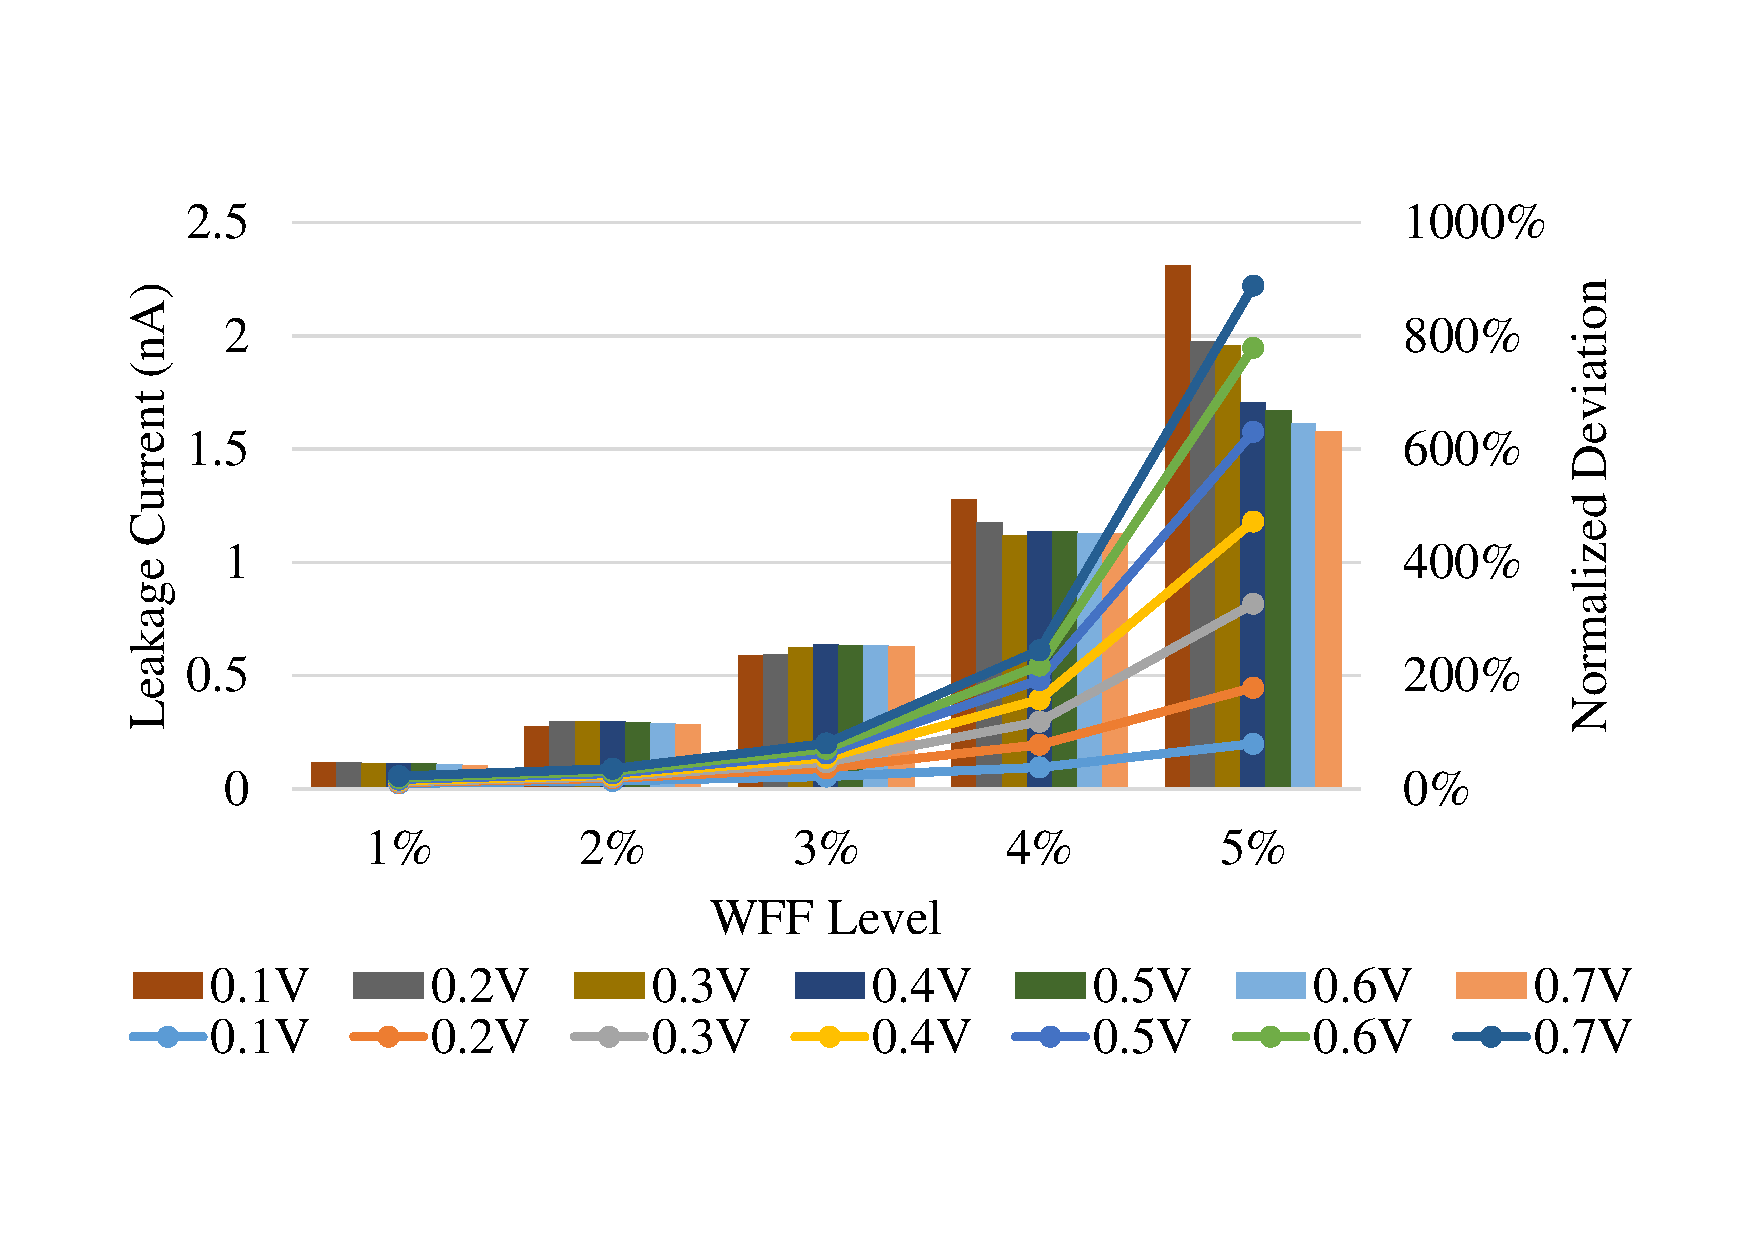
\includegraphics[width=0.9\textwidth, trim={1.25cm 3cm 2cm 3cm}, clip]{offCurrentComp.pdf}
    %        \caption{Leakage current scaling (left axis) and standard deviation (right axis) for the inverter.}
    %    \label{figsOffCurrComp}
    %\end{figure}



%Additionally, as stated in the last section, as the process variability level increases, the most recommended supply voltage, in order to achieve the highest robustness to variability effects on energy deviations, decreases.
%\vspace{0cm}

\section{Static Noise Margins}

	The SNM of a circuit should be as high as possible in order to provide more noise tolerance. The noise, is defined by any extraneous voltage amplitude added to the signal in consideration. The circuit noise tolerance is defined by the circuit ability to receive this extraneous voltage amplitude summed with the \textit{noise-free} signal without causing it output voltage to deviate from the allowable logic voltage level. In this case, the SNMs were measures considering each designs VTCs at different supply voltage levels. This characteristic becomes increasingly critical for low power devices, as supply voltage decreases and noise amplitudes which accounted for only a fraction of the device supply voltage, can now be comparable to the total value of the supply voltage.

	The evaluation of the SNMs are shown at Table \ref{tab:SNM}. The inverter and SIG presented identical SNMs. The TIST designs presented higher SNMs than the inverter and SIG at sub-threshold levels. The ST presented higher SNMs overall. In comparison to the inverter, SIG, and TIST 3:1 - which presented the same average SNM of 0.164V - the TIST 2:1 presented 2.6\% lower SNMs, while the ST showed 17.5\% higher SNMs. The ST presents the biggest differences at low supply voltages, with 41.91\% and 28.23\% higher SNMs at 0.1V and 0.2V, respectively, comparing to the inverter.

\begin{table}[H]
\centering
\caption{Static Noise Margins for each design as supply voltage scales.}
\label{tab:SNM}
\resizebox{0.9\textwidth}{!}{%
\begin{tabular}{|c|c|c|c|c|c|c|c|c|}
\hline
\multirow{2}{*}{Design} &
  \multirow{2}{*}{SNM (V)} &
  \multicolumn{7}{c|}{Supply Voltage (V)} \\ \cline{3-9}
 & & 0.1 & 0.2 & 0.3 & 0.4 & 0.5 & 0.6 & 0.7 \\ \hline
\multirow{3}{*}{INV}      & $NM_{L}$      & 0.025          & 0.074          & 0.122          & 0.171          & 0.217          & 0.253          & 0.277          \\ \cline{2-9}
		          & $NM_{H}$	  & 0.025          & 0.073          & 0.121          & 0.169          & 0.216          & 0.259          & 0.299	         \\ \cline{2-9}
		          & \textbf{Avg.} & \textbf{0.025} & \textbf{0.073} & \textbf{0.122} & \textbf{0.170} & \textbf{0.216} & \textbf{0.256} & \textbf{0.288} \\ \hline
\multirow{3}{*}{SIG}      & $NM_{L}$      & 0.025          & 0.074          & 0.122          & 0.171          & 0.217          & 0.253          & 0.277	         \\ \cline{2-9}
 	                  & $NM_{H}$      & 0.025          & 0.073          & 0.121          & 0.169          & 0.216          & 0.259          & 0.299          \\ \cline{2-9}
		          & \textbf{Avg.} & \textbf{0.025} & \textbf{0.073} & \textbf{0.122} & \textbf{0.170} & \textbf{0.216} & \textbf{0.256} & \textbf{0.288} \\ \hline
\multirow{3}{*}{ST}       & $NM_{L}$      & 0.036          & 0.111          & 0.178          & 0.244          & 0.310          & 0.376          & 0.440          \\ \cline{2-9}
 		          & $NM_{H}$      & 0.036          & 0.077          & 0.111          & 0.144          & 0.178          & 0.213          & 0.248          \\ \cline{2-9}
 		          & \textbf{Avg.} & \textbf{0.036} & \textbf{0.094} & \textbf{0.144} & \textbf{0.194} & \textbf{0.244} & \textbf{0.294} & \textbf{0.344} \\ \hline
\multirow{3}{*}{TIST 2:1} & $NM_{L}$      & 0.061          & 0.161          & 0.245          & 0.292          & 0.319          & 0.337          & 0.359          \\ \cline{2-9}
                          & $NM_{H}$      & 0.014          & 0.007          & 0.010          & 0.038          & 0.079          & 0.131          & 0.189          \\ \cline{2-9}
 			  & \textbf{Avg.} & \textbf{0.037} & \textbf{0.084} & \textbf{0.128} & \textbf{0.165} & \textbf{0.199} & \textbf{0.234} & \textbf{0.274} \\ \hline
\multirow{3}{*}{TIST 3:1} & $NM_{L}$      & 0.051          & 0.150          & 0.233          & 0.277          & 0.300          & 0.314          & 0.341          \\ \cline{2-9}
                          & $NM_{H}$      & 0.022          & 0.017          & 0.022          & 0.056          & 0.108          & 0.173          & 0.235          \\ \cline{2-9}
                          & \textbf{Avg.} & \textbf{0.036} & \textbf{0.084} & \textbf{0.128} & \textbf{0.167} & \textbf{0.204} & \textbf{0.244} & \textbf{0.288} \\ \hline
\end{tabular}%
}
\end{table}

\section{Output Gains and Slopes}

    \begin{figure}[t]
        \centering
            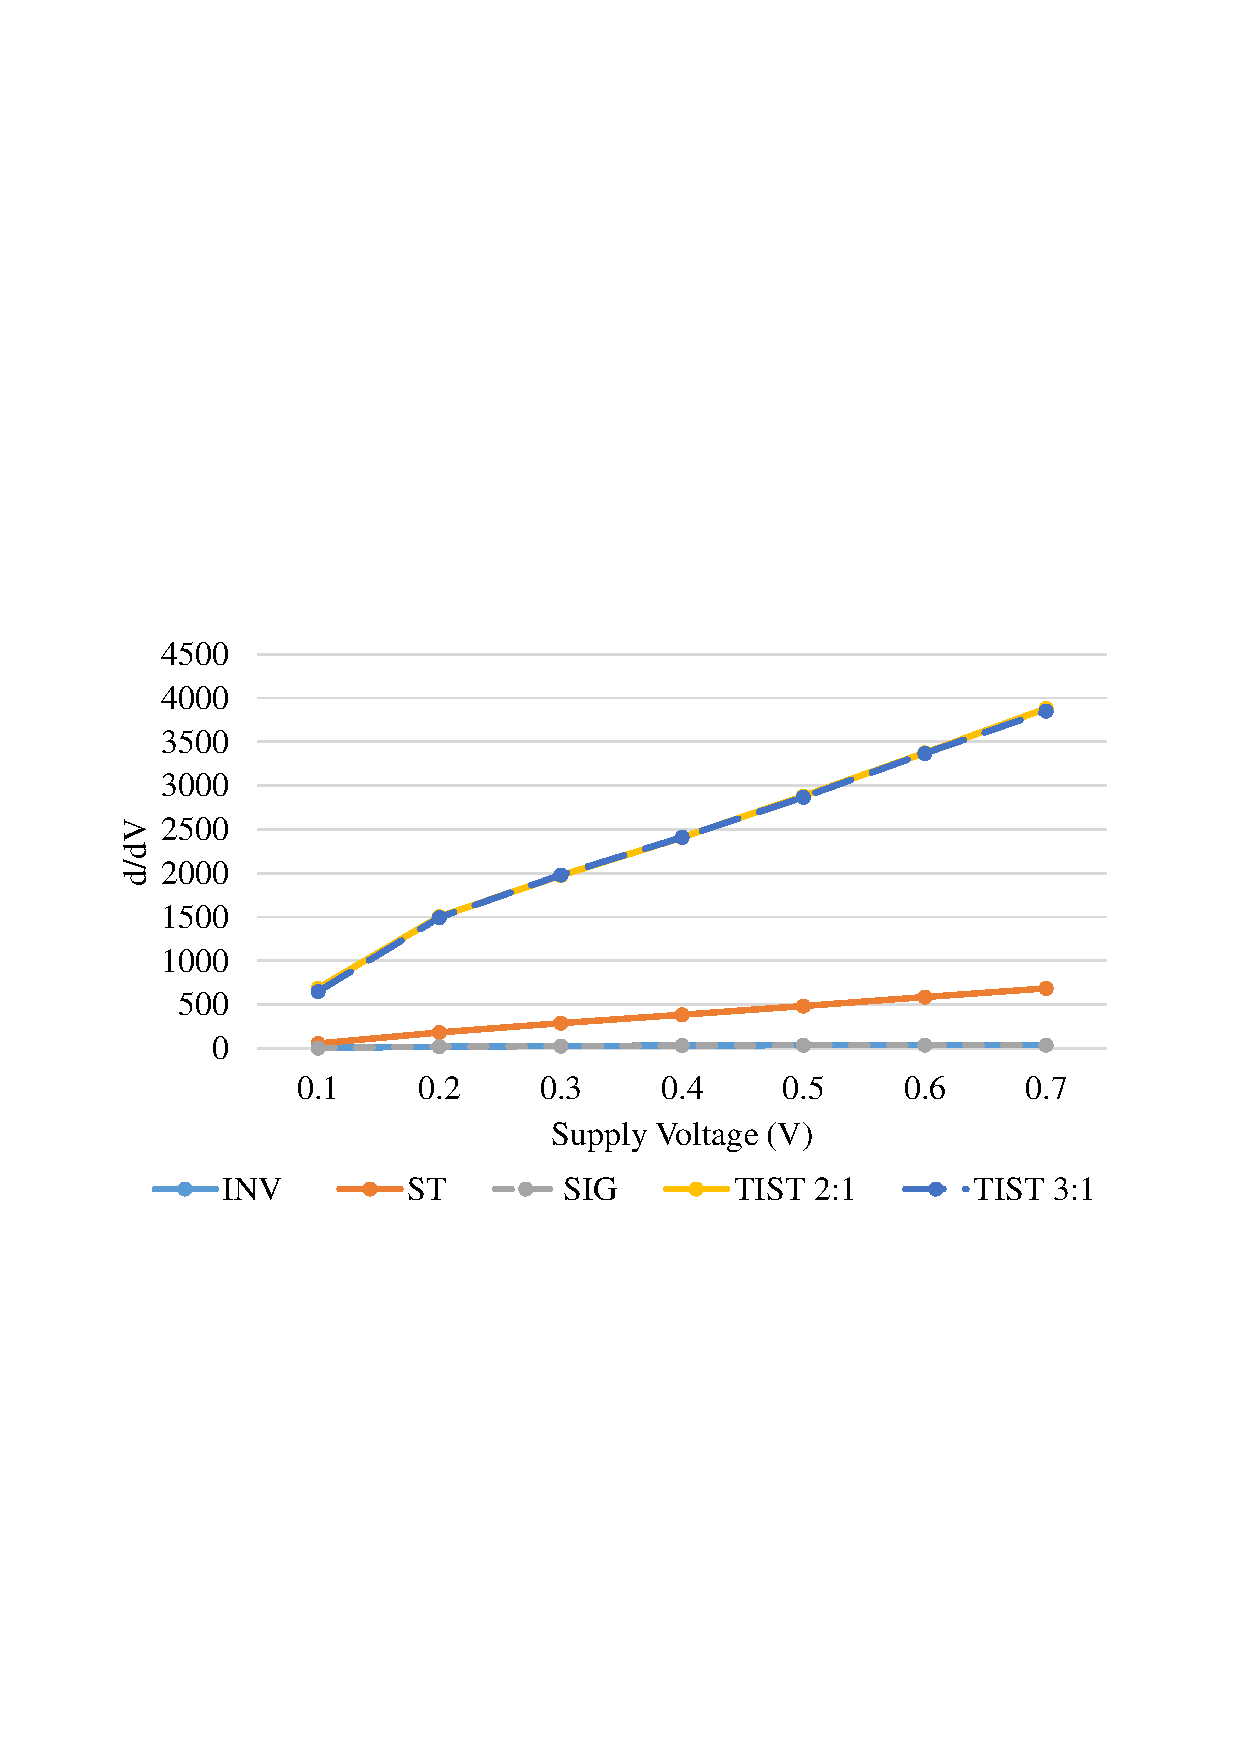
\includegraphics[width=0.8\textwidth, trim={1.25cm 9cm 2cm 10cm}, clip]{gainComp.pdf}
            \caption{Output gain value across voltage scaling.}
        \label{figsGainComp}
    \end{figure}

    \begin{figure}[h]
        \centering
            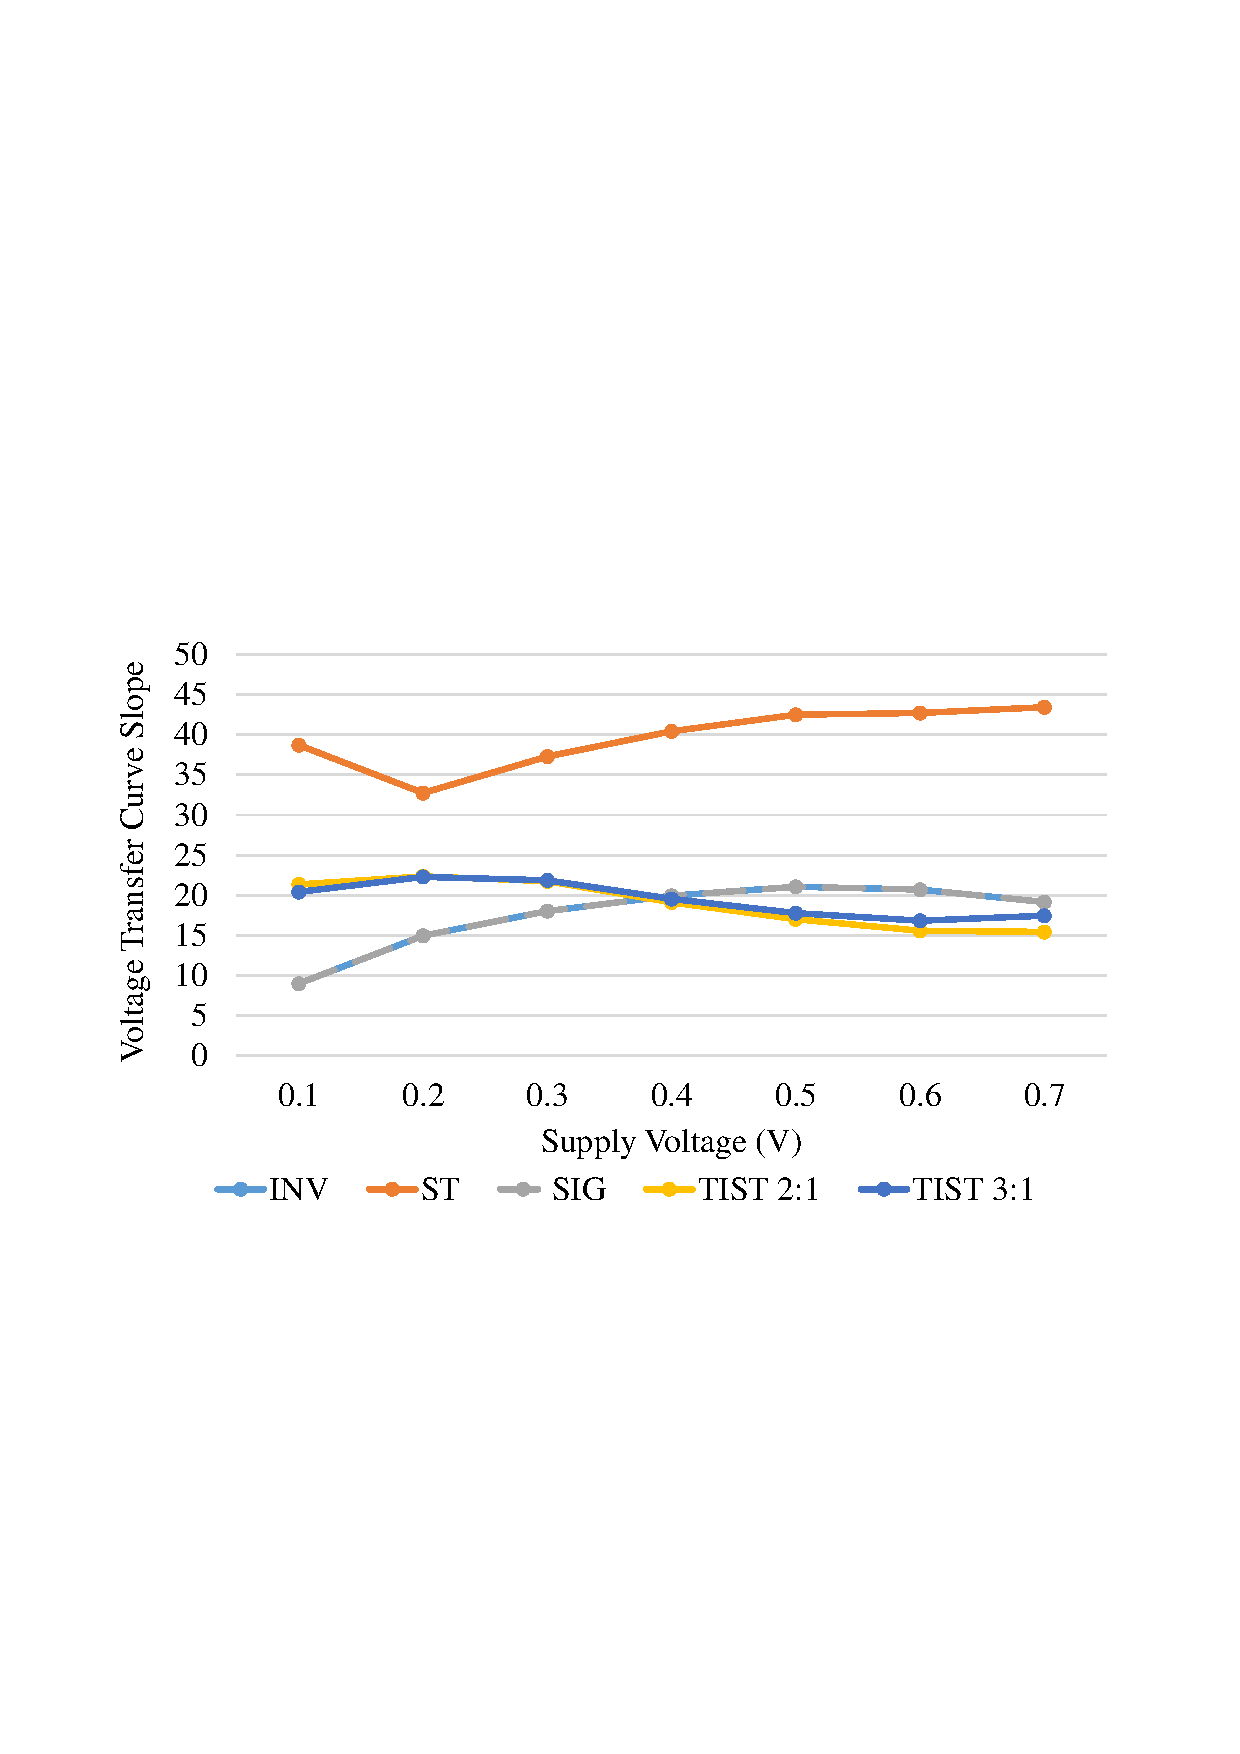
\includegraphics[width=0.8\textwidth, trim={1.25cm 9cm 2cm 10cm}, clip]{slopes.pdf}
            \caption{Voltage Transfer Curve slopes through supply voltage scaling for each design.}
        \label{fig:slopes}
    \end{figure}

The output gain and slopes will mainly determine how much and how fast the output will change and respond to changes in the intput. The gain will measure how much more the output will change its value in comparison to a small change in the input. The slopes will determine how fast the output takes to change its value. A circuit can present a high gain, which means that at a specific point in the VTC curve a small change in the input value is changing the output value drastically. Although, it can present low slope values as well, which means that the time the output takes to change its value is relatively high. In an ideal scenario, the circuit should show both high gains and slopes, making the change of its output as fast as possible, approaching its output signal to an ideal square signal.


It was considered the output gain values for each design, as show in Fig. \ref{figsGainComp}. These measures present the most broader difference across all designs. The TIST and ST designs presented, on average, values up to 8300.60\%, and 1246.50\% higher, respectively, in comparison to the inverter and SIG designs, which presented the same gains. Furthermore, the curve slope measures are shown in Fig. \ref{fig:slopes}, where lower slopes can be observed for the TIST, SIG and inverter designs in comparison to the ST. The ST and TIST designs presented 126.24\% and 9.43\% higher average slopes, respectively, in comparison to the inverter and SIG designs which showed identical measures. Figs. \ref{fig:vtcs01} and \ref{fig:vtcs07} show the VTC curves for all designs. It shows how the TIST although presenting higher gain, present lower slopes, given that it takes more time to properly discharge.


    \begin{figure}[H]
        \centering
            \includegraphics[width=1\textwidth, trim={0cm 0cm 0cm 0cm}, clip]{vtcs01.png}
            \caption{Voltage Transfer Curves for all designs at 0.1V.}
        \label{fig:vtcs01}
    \end{figure}

        \begin{figure}[H]
        \centering
            \includegraphics[width=1\textwidth, trim={0cm 0cm 0cm 0cm}, clip]{vtcs07.png}
            \caption{Voltage Transfer Curves for all designs at 0.7V.}
        \label{fig:vtcs07}
    \end{figure}
    %According to \cite{henzler2006power}

\section{Hysteresis}

The hysteresis characteristic, for the designs who present it through circuit-level methods, will improve the circuit noise margins through the insertion of upper and lower threshold voltages. The hysteresis does not improve the noise margins through enhancing the signal - by making it closer to an ideal square signal - although, through the two threshold voltages, it will make necessary higher noise amplitude in order to kickoff the value change of the output signal.

    The hysteresis ratios measures for all designs, which present hysteresis, are shown in Fig. \ref{figsHystComp}. The hysteresis ratio is the ratio between the hysteresis interval (V) and the supply voltage (V), which will result in a percentage of the current supply voltage. Given so, the TIST designs presented higher average ratios of 18.92\% and 15.95\% for the 2:1 and 3:1 designs, respectively, with the ST presenting an average ratio of 8.62\%. It is important to highlight the ratio losses as well, the TIST designs presented ratio decreases up to 14.68\% and the ST presented a better response with a 5.68\% decrease. The hysteresis curves for all designs at nominal supply voltage are shown in Fig. \ref{fig:hystCurves}. Furthermore, the hysteresis ratios in relation to the supply voltage are shown in Fig. \ref{fig:hystRatiosVdd}, it can be observed huge hysteresis intervals for the TIST designs, which are responsible for the circuit failing working at acceptable frequencies.

%por que diminui?

%since due to the variability scaling and its related increase on off-current, the ratios will tend to decrease. This result is due to the leakage current supression embedded into the ST design through the feed-back system. Therefore,
%In order to tackle this problem, further increase of the ratio between the TIST inverter and latch transistors sizes would be necessary, inserting even higher area penalties.

    \begin{figure}[H]
        \centering
            \includegraphics[width=0.8\textwidth, trim={1.25cm 9cm 2cm 10cm}, clip]{hystWFFComp.pdf}
            \caption{Design hysteresis ratio comparison (left) and hysteresis ratio normalized deviation (right), across variability scaling.}
        \label{figsHystComp}
    \end{figure}

    \begin{figure}[H]
        \centering
            \includegraphics[width=0.8\textwidth, trim={2cm 3cm 2cm 3cm}, clip]{hystGraphs.pdf}
            \caption{Hysteresis curves for all designs at nominal supply voltage.}
        \label{fig:hystCurves}
    \end{figure}

    \begin{figure}[H]
        \centering
            \includegraphics[width=0.8\textwidth, trim={2cm 3cm 2cm 3cm}, clip]{hystRatiosVdd.pdf}
            \caption{Design hysteresis ratios comparison across supply voltage scaling.}
        \label{fig:hystRatiosVdd}
    \end{figure}

    The average hysteresis ratio deviations for each design was 23.44\%, 24.83\%, and 27.30\% for the ST, TIST 2:1 and TIST 3:1. The hysteresis average ratio deviation measures did not present considerable differences between designs, although, at high variability scenarios (5\% WFF) the ST presented 16.79\% and 21.40\% lower deviations, in comparison to the TIST 2:1 and TIST 3:1, respectively.

\section{Measures Distribution}

    Fig. \ref{fig:energyDist0_2} shows the distribution of the energy metrics for the inverter over all levels of WFF for 0.2V, 0.4V, and 0.7V supply voltages. Each figure presents an histogram of the 2000 simulations with a blue line, indicating where the average energy measure is located at. The black line corresponds to a projection of the local average. For low variability and high supply voltage scenarios it can be observed a normal, or close-to-normal, distribution. At higher variability and lower supply voltages, a right skew can be noted at first, where the majority of the cases stay clustered although, there are a considerable number of cases where the energy is lower than the average. As variability rises even further, the skew direction will shift and take a hard left, with the worst scenarios showing up to 5 orders of magnitude higher than the average. Histograms and dispersion graphs for all designs, are shown in Appendix C.

     \begin{figure}[]
        \centering
            \includegraphics[width=1.5\textwidth, trim={0cm 0cm 0cm 0cm}, clip, angle=270]{dist_energy_0_2.pdf}
            \caption{Energy measures distribution for the inverter at different levels of variability and supply voltage.}
        \label{fig:energyDist0_2}
    \end{figure}

    %\begin{figure}[]
    %    \centering
    %        \includegraphics[width=1\textwidth, trim={0cm 0cm 0cm 0cm}, clip]{dist_energy_INV_0_4.pdf}
    %        \caption{Energy measures distribution for the inverter at different levels of variability at 0.4V.}
    %    \label{fig:energyDist0_4}
    %\end{figure}

    %     \begin{figure}[]
    %    \centering
    %        \includegraphics[width=1\textwidth, trim={0cm 0cm 0cm 0cm}, clip]{dist_energy_INV_0_7.pdf}
    %        \caption{Energy measures distribution for the inverter at different levels of variability at 0.7V.}
    %    \label{fig:energyDist0_7}
    %\end{figure}

\chapter{Full Adders}

%\section{Full Adders}

The results are divided into two main analyses, with the set of FAs operating at nominal and near-threshold. In both cases, simulations were performed with and without the ST technique. To better present the improvements (positive values) and drawbacks (negative values) of each ST, results also show a comparison ($\Delta$) between the normalized deviation between the traditional and the circuits with the applied technique. For the sake of simplicity the LPST and traditional 6T ST were renamed ST1 and ST2, respectively.

\section{Nominal Operation}

The results concerning propagation times at nominal levels are show in Table \ref{delayNominal}. It is possible to observe no considerable improvement over variability robustness concerning the propagation times. It can be explained due to the pass-transistor logic present in the TFA, TGA, and Hybrid given further signal degradation as a result of the area and parasitics increase. Furthermore, it can be observed only a slight improvement over the Mirror FA given its mirroring-based logic with many paths to source and ground.

For the energy results, it was observed considerable improvement over robustness in the Mirror, TFA, and TGA, as shown in Table \ref{energiaNominal}. There was a considerable worsening over the Hybrid energy robustness. It is mainly due to its number of transistors, which is comparable to the Mirror FA but it is not entirely based on complementary logic, and the four internal inverters replaced, which , further increasing its area and signal degradation. Overall, the traditional TFA presented the best performance and, by far, the lowest energy consumption and energy normalized deviation at nominal operation. However, it presented the highest delay deviations.

%\setlength\tabcolsep{2 pt}

%%DELAYS NOMINAL
\begin{table}[]
\centering
\caption{Delay measures for nominal voltage operation}
\label{delayNominal}
\resizebox{\textwidth}{!}{%
\begin{tabular}{lccccccccc}
\hline
\multirow{3}{*}{FA} & \multirow{3}{*}{ST} & \multicolumn{8}{c}{Delays} \\ \cline{3-10}
 & &  \multicolumn{4}{c}{SUM} & \multicolumn{4}{c}{CARRY OUT} \\ \cline{3-10}
 & & \textbf{$\mu$(ps)} & \textbf{$\sigma$(ps)} & \textbf{$\sigma$/$\mu$(\%)} & \textbf{$\Delta$(\%)} & \textbf{$\mu$(ps)} & \textbf{$\sigma$(ps)} & \textbf{$\sigma$/$\mu$(\%)} & \textbf{$\Delta$(\%)} \\ \hline
\multirow{3}{*}{Mirror} & - & 22.83 & 4.82 & 20.89 & - & 22.60 & 4.39 & 19.38 & - \\ \cline{2-10}
 & ST1 & 27.38 & 5.75 & 20.77 & 0.54 & 25.31 & 4.79  & 18.87 & 2.63 \\ \cline{2-10}
 & ST2 & 42.28 & 8.57 & 20.23 & 3.13 & 41.48 & 7.96 & 19.17 & 1.10 \\ \hline
\multirow{3}{*}{TFA} & - & 20.76 & 5.51 & 30.69 & - & 19.75 & 4.70 & 25.74 & - \\ \cline{2-10}
 & ST1 & 24.24 & 6.43 & 31.42 & -2.37 & 22.50 & 5.51 & 26.74 & -3.86 \\ \cline{2-10}
 & ST2 & 42.36 & 76.87 & 126.26 & -311.36 & 26.91 & 6.86 & 31.45 & -22.18 \\ \hline
\multirow{3}{*}{TGA} & - & 21.56 & 4.30 & 22.36 & - & 22.96 & 4.70  & 20.46 & - \\ \cline{2-10}
& ST1 & 25.32 & 5.36 & 26.42 & -18.16  & 26.39 & 5.41  & 20.38 & 0.37 \\ \cline{2-10}
& ST2 & 97.92 & 210.62 & 102.35 & -357.80 & 32.80 & 7.85 & 25.70 & -25.63 \\ \hline
\multirow{3}{*}{Hybrid} & - & 24.02 & 5.31 & 21.75 & - & 23.58 & 4.89  & 21.65 & - \\ \cline{2-10}
& ST1 & 60.96 & 64.91 & 92.40 & -324.90 & 42.07 & 21.84 & 34.84 & -60.90 \\ \cline{2-10}
& ST2 & 69.68 & 40.87 & 50.82 & -133.72 & 72.05 & 25.81 & 29.23 & -35.00 \\ \hline
\end{tabular}%
}
\end{table}

%%ENERGIA NOMINAL
\begin{table}[]
\centering
\caption{Energy measures for nominal voltage operation}
\label{energiaNominal}
\resizebox{\textwidth}{!}{%
\begin{tabular}{lccccccccc}
\hline
\multirow{3}{*}{FA} & \multirow{3}{*}{ST} & \multicolumn{8}{c}{Energy} \\ \cline{3-10}
 & & \multicolumn{4}{c}{SUM} & \multicolumn{4}{c}{CARRY OUT} \\ \cline{3-10}
 & & \textbf{$\mu$(fJ)} & \textbf{$\sigma$(fJ)} & \textbf{$\sigma$/$\mu$(\%)} & \textbf{$\Delta$(\%)} & \textbf{$\mu$(fJ)} & \textbf{$\sigma$(fJ)} & \textbf{$\sigma$/$\mu$(\%)} & \textbf{$\Delta$(\%)} \\ \hline
\multirow{3}{*}{Mirror} & - & 19.30 & 3.55 & 18.35 & - & 27.30 & 3.99 & 14.60 & - \\ \cline{2-10}
& ST1 & 26.80 & 4.85 & 18.10 & 1.37 & 37.20 & 5.54 & 14.87 & -1.84 \\ \cline{2-10}
& ST2 & 36.50 & 5.50 & 15.07 & 17.87 & 50.80 & 6.54 & 12.87 & 11.84 \\ \hline
\multirow{3}{*}{TFA} & - & 4.97 & 1.27 & 25.59 & - & 5.15 & 0.72 & 13.91 & - \\ \cline{2-10}
& ST1 & 10.90 & 1.46 & 13.38 & 47.70 & 10.80 & 0.98 & 9.09 & 34.68 \\ \cline{2-10}
& ST2 & 17.00 & 2.02 & 11.94 & 53.35 & 15.30 & 2.02 & 13.21 & 5.05 \\ \hline
\multirow{3}{*}{TGA} & - & 14.10 & 3.81 & 27.07 & - & 15.70 & 4.44 & 28.20 & - \\ \cline{2-10}
& ST1 & 24.90 & 6.33 & 25.46 & 5.95 & 26.40 & 4.21 & 15.94 & 43.48 \\ \cline{2-10}
& ST2 & 32.40 & 7.49 & 23.16 & 14.44 & 37.60 & 7.35 & 19.53 & 30.74 \\ \hline
\multirow{3}{*}{Hybrid} & - & 19.30 & 4.10 & 21.26 & - & 26.30 & 4.55 & 17.29 & - \\ \cline{2-10}
& ST1 & 72.50 & 37.95 & 52.34 & -146.19 & 94.60 & 48.21 & 50.94 & -194.62 \\ \cline{2-10}
& ST2 & 73.20 & 21.25 & 29.05 & -36.64 & 95.20 & 19.89 & 20.90 & -20.88 \\ \hline
\end{tabular}%
}
\end{table}

\section{Near-Threshold Operation}

 At near-threshold operation the noise margins are decreased. Given so, the designs make full use of the higher SNMs of the STs, as shown in Table \ref{delayNT}. It can be observed a superior robustness improvement with the ST2, given its smaller area, and consequently, lower signal degradation. In the case of the TFA it seems that due to its few paths to source and ground, the higher parasitic capacitance and resistance present in ST2 brings higher deviation, with the ST1 presenting better results.

 For the energy results, shown in Table \ref{energiaNT}, ST1 showed superior robustness improvement for the TFA and TGA, which can be explained by their pass-transistor based logic and the ST1 smaller parasitics, in comparison to the Mirror and Hybrid FAs which showed no improvement whatsoever.

 For the delay results, the Mirror FA showed the lowest means and normalized deviations, which is expected given it is not based on pass-transistor logic, having better driving capabilities. For the energy measures, TFA showed the lowest mean, due to its pass-transistor logic and lower number of transistors. Although, the TFA presented the highest delay normalized deviations. Overall, the TGA showed the lowest normalized deviations in energy and the highest robustness gains concerning delay and energy measures.

%%DELAYS NT
\begin{table}[]
\centering
\caption{Delay measures for near-threshold operation}
\label{delayNT}
\begin{tabular}{lccccccccc}
\hline
\multirow{3}{*}{FA} & \multirow{3}{*}{ST} & \multicolumn{8}{c}{Delays} \\ \cline{3-10}
& & \multicolumn{4}{c}{SUM} & \multicolumn{4}{c}{CARRY OUT} \\ \cline{3-10}
& & \textbf{$\mu$(ps)} & \textbf{$\sigma$(ps)} & \textbf{$\sigma$/$\mu$(\%)} & \textbf{$\Delta$(\%)} & \textbf{$\mu$(ps)} & \textbf{$\sigma$(ps)} & \textbf{$\sigma$/$\mu$(\%)} & \textbf{$\Delta$(\%)} \\ \hline
\multirow{3}{*}{Mirror} & - & 103.49 & 63.18 & 60.95 & - & 91.62 & 55.41 & 59.18 & - \\ \cline{2-10}
& ST1 & 119.98 & 67.63 & 56.09 & 7.97 & 115.50 & 73.68 & 64.11 & -8.32 \\ \cline{2-10}
& ST2 & 155.58 & 67.03 & 42.94 & 29.55 & 153.50 & 68.89 & 44.86 & 24.20 \\ \hline
\multirow{3}{*}{TFA} & - & 122.48 & 117.46 & 111.51 & - & 111.64 & 186.41 & 236.88 & - \\ \cline{2-10}
& ST1 & 142.18 & 146.61 & 97.85 & 12.25 & 118.26 & 194.03 & 242.22 & -2.26 \\ \cline{2-10}
& ST2 & 215.93 & 222.26 & 117.29 & -5.18 & 165.48 & 335.16 & 273.57 & -15.49 \\ \hline
\multirow{3}{*}{TGA} & - & 130.43 & 109.19 & 85.78 & - & 114.78 & 130.53 & 138.93 & - \\ \cline{2-10}
& ST1 & 122.99 & 98.03 & 79.75 & 7.03 & 128.98 & 101.51 & 88.48 & 36.32 \\ \cline{2-10}
& ST2 & 187.84 & 125.13 & 70.99 & 17.25 & 164.06 & 109.19 & 72.68 & 47.68 \\ \hline
\multirow{3}{*}{Hybrid} & - & 115.90 & 83.02 & 70.57 & - & 111.92 & 82.45 & 74.76 & - \\ \cline{2-10}
& ST1 & 187.36 & 143.80 & 78.99 & -11.93 & 116.02 & 71.26 & 61.00 & 18.41 \\ \cline{2-10}
& ST2 & 207.00 & 168.04 & 72.56 & -2.81 & 167.50 & 66.72 & 40.94 & 45.23 \\ \hline
\end{tabular}
\end{table}
\vspace{1em}
%ENERGIA NT

\begin{table}[]
\centering
\caption{Energy measures for near-threshold operation}
\label{energiaNT}
\begin{tabular}{lccccccccc}
\hline
\multirow{3}{*}{FA} & \multirow{3}{*}{ST} & \multicolumn{8}{c}{Energy} \\ \cline{3-10}
& & \multicolumn{4}{c}{SUM} & \multicolumn{4}{c}{CARRY OUT} \\ \cline{3-10}
& & \textbf{$\mu$(fJ)} & \textbf{$\sigma$(fJ)} & \textbf{$\sigma$/$\mu$(\%)} & \textbf{$\Delta$(\%)} & \textbf{$\mu$(fJ)} & \textbf{$\sigma$(fJ)} & \textbf{$\sigma$/$\mu$(\%)} & \textbf{$\Delta$(\%)} \\ \hline
\multirow{3}{*}{Mirror} & - & 10.10 & 3.04 & 30.12 & - & 14.10 & 2.53 & 18.00 & - \\ \cline{2-10}
& ST1 & 13.90 & 4.05 & 29.07 & 3.50 & 18.60 & 4.25 & 22.93 & -27.42 \\ \cline{2-10}
& ST2 & 18.40 & 4.34 & 23.60 & 21.64 & 25.30 & 5.73 & 22.59 & -25.53 \\ \hline
\multirow{3}{*}{TFA} & - & 2.62 & 0.83 & 31.49 & - & 2.71 & 0.37 & 13.49 & - \\ \cline{2-10}
& ST1 & 5.67 & 1.34 & 23.69 & 24.76 & 5.69 & 0.63 & 11.01 & 18.38 \\ \cline{2-10}
& ST2 & 9.69 & 2.11 & 21.74 & 30.96 & 8.80 & 2.59 & 29.40 & -117.89 \\ \hline
\multirow{3}{*}{TGA} & - & 6.87 & 1.56 & 22.68 & - & 8.11 & 2.90 & 35.70 & - \\ \cline{2-10}
& ST1 & 12.90 & 2.37 & 18.45 & 18.65 & 13.50 & 1.86 & 13.79 & 61.37 \\ \cline{2-10}
& ST2 & 16.10 & 3.09 & 19.17 & 15.48 & 17.30 & 2.57 & 14.86 & 58.38 \\ \hline
\multirow{3}{*}{Hybrid} & - & 9.66 & 3.09 & 32.02 & - & 12.80 & 3.17 & 24.77 & - \\ \cline{2-10}
& ST1 & 36.40 & 17.94 & 49.30 & -53.96 & 45.80 & 23.63 & 51.54 & -108.07 \\ \cline{2-10}
& ST2 & 35.40 & 12.72 & 35.91 & -12.14 & 46.60 & 13.84 & 29.69 & -19.86 \\ \hline
\end{tabular}
\end{table}

%\vspace{-1.5em}

\section{Penalties}

Overviews for metrics measurements and variability sensitivities are shown in Figs. \ref{fig:avgDelayNominal}, \ref{fig:avgEnergyNominal}, \ref{fig:avgDelayNT}, and \ref{fig:avgEnergyNT}. Since it is considered a technique where a single inverter (2 transistors) by ST1/ST2 (4/6 transistors). It is expected penalties concerning delay, energy and area metrics. For the delays, it was observed an average 30\% and 97\% increase for the ST1 and ST2, respectively. Additionally, for the energy, there was a 123\% and 176\% average increase for the ST1 and ST2, respectively.

Concerning area penalties, the ST1 increased the FAs area by 157.71\%, on average, while the ST2 increased by 52.20\%. The ST1 higher increase in area is due to the necessity to use TAP-Cells, which is a technology restriction, in order to explicitly connect the transistor's bulk to specific points of the circuit or source/ground making the ST1 cell more prominent than expected. The ST2 does not apply specific bulk connections, although it was necessary the use of METAL3 for cell routing, increasing parasitic capacitance and resistance.

Considering all scenarios, there can be observed no delay robustness improvement at nominal operation with the ST1 and ST2 showing, on average, 50\% and 115.2\% worsening on delay robustness, respectively. For energy robustness, at nominal operation, the ST2 presented a considerable average improvement of 11.18\% while the ST1 showed an average worsening of 25\%. For near-threshold operation, ST1 and ST2 showed 7.79\% and 18.173\% higher delay robustness. For energy robustness, the ST2 showed a 4.13\% improvement while the ST1 presented a worsening of 4.5\%.

%\vspace{-3.65em}

\begin{figure}[]
  \centering
    \includegraphics[width=0.85\textwidth, trim={2cm 10cm 2cm 10.5cm}, clip]{averageDelayNominal.pdf}
     \caption{Average delay measures for nominal operation and their respective normalized deviation (variability sensitivity).}
  \label{fig:avgDelayNominal}
\end{figure}

%\vspace{1em}

\begin{figure}[]
  \centering
    \includegraphics[width=0.85\textwidth, trim={3.5cm 3cm 2cm 3.5cm}, clip]{averageEnergyNominal.pdf}
     \caption{Average energy measures for nominal operation and their respective normalized deviation (variability sensitivity).}
  \label{fig:avgEnergyNominal}
\end{figure}

%\vspace{1em}

\begin{figure}[]
  \centering
    \includegraphics[width=0.85\textwidth, trim={3.5cm 3cm 2cm 3.5cm}, clip]{averageDelayNT.pdf}
     \caption{Average delay measures for near-threshold operation and their respective normalized deviation (variability sensitivity).}
  \label{fig:avgDelayNT}
\end{figure}

%\vspace{1em}

\begin{figure}[]
  \centering
    \includegraphics[width=0.85\textwidth, trim={3.5cm 3cm 2cm 3.5cm}, clip]{averageEnergyNT.pdf}
     \caption{Average energy measures for near-threshold operation and their respective normalized deviation (variability sensitivity).}
  \label{fig:avgEnergyNT}
\end{figure}

\chapter{Conclusions}

The ongoing trend of IoT devices was enabled by two key technology improvements: battery lifetime through capacity improvement, and node scaling. Although, for specific applications, battery maintenance and charging through the power grid is not possible. Given so, IoT devices have been constrained with tight energy consumption metrics, and adapted with self-sufficient mechanisms in order to produce energy through external sources. The node scaling, that enabled IoT devices, comes not short of inherent challenges, with process variability being the major one. New transistor technologies have been proposed such as FinFETs, although even such devices, at deep submicron nodes (e.g. 7-nm), present considerable deviation in its metrics. Such deviations are not appropriate for such sensible devices working at narrow constraints (with energy consumption being a priority).

Given so, an analysis over multiple scenarios considering several levels of process variability, supply voltages, and transistor sizing was performed in order to identify the adequate fin number and supply voltage for various kinds of inverter circuits prioritizing energy consumption and the minimization of deviations. Furthermore, the impact of the replacement of Full Adders internal inverters was analyzed considering two types of Schmitt Trigger and four types of Full Adders.

An overview for the inverter designs analysis is shown in Table \ref{tab:overview}, where the designs with the highest average and normalized standard deviations for each metric are presented. On performance, the inverter presented the lowest propagation times, and lowest frequency loss due to variability impact. Although, it presented the higher propagation deviations than the ST and SIG designs. The ST and SIG designs presented the lowest frequencies, but lowest propagation times deviations as well. The TIST 2:1 designs presented frequencies on average lower to the ST and SIG designs, and higher deviations, second only to the 3:1 designs which presented higher frequencies, apart from the inverter, than all of the designs. Given so, it can be observed the higher impact of variability on the TIST designs which present the lowest average frequencies (for the 2:1 TISTs) and second highest frequencies (for the 3:1 TISTs) and still presented considerable higher propagation deviations in comparison to all designs.

% Please add the following required packages to your document preamble:
% \usepackage{multirow}
% \usepackage{graphicx}
\begin{table}[]
\centering
\caption{Overall results overview for all designs.}
\label{tab:overview}

\resizebox{0.75\textwidth}{!}{%
\begin{tabular}{|c|c|c|c|}
\hline
Metric                            &         & Average     & Deviations \\ \hline
\multirow{2}{*}{Delays}           & Highest & TIST 2:1     & TIST 3:1   \\ \cline{2-4}
                                  & Lowest  & INV          & SIG        \\ \hline
\multirow{2}{*}{Energy}           & Highest & TIST 2:1     & TIST 2:1   \\ \cline{2-4}
                                  & Lowest  & INV          & INV        \\ \hline
\multirow{2}{*}{SNMs}             & Highest & ST           & -          \\ \cline{2-4}
                                  & Lowest  & TIST 2:1     & -          \\ \hline
\multirow{2}{*}{Current Ratios}   & Highest & TIST 2:1     & TIST 2:1   \\ \cline{2-4}
                                  & Lowest  & SIG          & ST         \\ \hline
\multirow{2}{*}{Gain}             & Highest & TIST         & -          \\ \cline{2-4}
                                  & Lowest  & INV/SIG      & -          \\ \hline
\multirow{2}{*}{Slope}            & Highest & ST           & -          \\ \cline{2-4}
                                  & Lowest  & TIST/INV/SIG & -          \\ \hline
\multirow{2}{*}{Hysteresis Ratio*} & Highest & TIST 2:1     & TIST 3:1   \\ \cline{2-4}
                                  & Lowest  & ST           & ST         \\ \hline
\end{tabular}%
}
\legend{*The inverter and SIG designs do not present a hysteresis characteristic.}
\end{table}

Trying to detect the most adequate values for the supply voltage and sizing variables for each type of application, low energy consumption, high robustness, and cost-benefit, a subset of solutions was chosen considering each level of variability. For the low energy applications, the inverter, ST, and SIG remained tightly together while the TIST designs presented way higher energy consumption. The high robustness application stayed favorable for the TIST designs, although not being directly comparable since it utilizes 2 to 3 times higher number of fins, and a higher supply voltage, to maintain such results. Putting the TIST designs aside, the ST design presents lower deviation, at the cost of much higher energy consumption for low variality scenarios. Therefore the SIG presents itself as an alternative, showing lower deviations and energy consumption similar to the inverter in the remaining cases. Although, it is important to highlight that the maximum energy deviation presented for this type of application was approximately 10\%.

Lastly, for the cost-benefit applications, the TIST designs maintained the lowest deviations, 73\% to 30\% lower than the inverter, at the cost of roughly 3.5 to 4.8 times higher energy consumption in comparison to the inverter. The SIG presented similar energy consumption (20\% higher) with a slight decrease on the deviations (8\%) in comparison to the inverter. Therefore, the inverter and SIG designs are still good alternatives, with the TIST designs tending more to a high robustness application with no to little restraints into energy consumption. The EDP over all chosen layouts, for each considered application, is shown at Table \ref{tab:edpApp}.

\begin{table}[]
\centering
\caption{EDP for each chosen design for the considered applications.}
\label{tab:edpApp}
\resizebox{0.7\textwidth}{!}{%
\begin{tabular}{|c|c|c|c|}
\hline
\multirow{2}{*}{Design} & \multicolumn{3}{c|}{EDP}                    \\ \cline{2-4}
                        & Low Energy & High Robustness & Cost Benefit \\ \hline
INV                     & 0.155      & 0.029           & 0.027        \\ \hline
ST                      & 0.124      & 0.112           & 0.053        \\ \hline
SIG                     & 0.114      & 0.037           & 0.031        \\ \hline
TIST 2:1                & 0.273      & 0.096           & 0.076        \\ \hline
TIST 3:1                & 0.214      & 0.113           & 0.086        \\ \hline
\end{tabular}%
}
\end{table}


When considering the current measures and deviations, the TIST designs presented the highest ratio, which is directly related to their transistor proportions. The ST presented a ratio more than two times higher than the inverter and SIG designs, while still maintaining a 1:1 transistor ratio and presenting the lowest ratio deviations. Due to the higher increase in the leakage in comparison to the dynamic current, all designs presented current ratio decreases over variability level scaling. The TIST designs presented lower decreases with the other considered designs presenting over 3x higher ratio declines. Over each specific current the ST and TIST designs presented considerably lower deviations on the dynamic current and minor improvements over leakage current deviations.

Concerning reliability over signals, the ST and TIST designs presented similar results at low supply voltages with widening differences as the supply voltage scaled up, with the ST presenting the highest noise margins and the TIST designs leveling up with the SIG and inverter designs which presented identical results through all supply voltage values. The TIST designs presented much higher gains, although presenting signal slopes comparable to the SIG and inverter designs, with the ST showing the highest signal slopes. Lastly, over the hysteresis ratios, the TIST designs presented a broad difference in comparison to the ST, although with higher deviations in most cases. Considering the hysteresis ratio scaling in comparison to the supply voltage, the TIST designs keep showing higher ratios (mainly at the lowest supply voltages), although due to higher ratios at near-threshold voltages the TIST circuits did not work properly at those specific levels of supply.

The impact of the ST1 and ST2 replacement of Full Adders internal inverters showed overall no improvement over delay deviations at nominal levels with a worsening up to 199.08\%, on average. On the contrary, for the energy measures the pass-transistor logic based Full Adders presented improvements up to 43.12\%, on average. At near-threshold operation, almost all designs take advantage of the gain improvement characteristic of the STs and showed a maximum of 36.07\% and 44.78\% lower deviations on the delays and energy metrics, respectively. Such results show that the more apropriate application of the technique is at near-threshold operating circuits and that, depending of the logic of which the Full Adder is based, it will present better or worse results with the area and transistor count having an influence as well, where the Hybrid Full Adder, one the of the biggest design with one of the highest transistor counts, presented almost no improvement.

Table \ref{tab:overallFAs} shows the best and worst cases concerning the metrics, and the two levels of supply voltage considered in the experiments. It can be observed the presence of the TFA at nominal level, presenting most of the lowest measures, which comes along with the TFA also presenting the smallest transistor count of all considered designs, making it the most apropriate Full Adder at nominal operation. On the other side, the Hybrid presented the worst results and has the biggest area overall, making it not very suitable, not only for nominal operation but for near-threshold operation as well. At near-threshold the TFAST2 presents itself with the highest delays and delay variations. Although, for the energy measures, its traditional version presents the lowest energy consumption and acceptable variations, although now as low as the TGAST1. Into the performance, the Mirror presented the best results.

\begin{table}[]
\centering
\caption{Best and worst cases considering all metrics and the two types of operation considered in the experiments.}
\label{tab:overallFAs}
\resizebox{0.95\textwidth}{!}{%
\begin{tabular}{|c|c|c|c|c|c|}
\hline
\multicolumn{2}{|c|}{\multirow{2}{*}{Operation}} & \multicolumn{2}{c|}{Delay} & \multicolumn{2}{c|}{Energy} \\ \cline{3-6}
\multicolumn{2}{|c|}{}             & Absolute  & Deviation & Absolute  & Deviation \\ \hline
\multirow{2}{*}{Nominal} & Highest & HYBRIDST2 & TFAST2    & HYBRIDST2 & HYBRIDST1 \\ \cline{2-6}
                         & Lowest  & TFA       & MirrorST2 & TFA       & TFAST1    \\ \hline
\multirow{2}{*}{NT}      & Highest & TFAST2    & TFAST2    & HYBRIDST1 & HYBRIDST1 \\ \cline{2-6}
                         & Lowest  & Mirror    & MirrorST2 & TFA       & TGAST1    \\ \hline
\end{tabular}%
}
\end{table}

Additionally, since when considering just one variable much of the impact of other variables are put aside, Table \ref{tab:edpddp} shows the layouts which presented the highest and lowest Measure Deviation Products (MDP), where the absolute value of the measures and its deviation are multiplied. This further analysis permits to consider not only one separable variable (e.g. only the absolute value or the deviation) but the impact of several measures into one index. Furthermore, in order to give the most overall apropriate layout, considering energy and delay measures and deviations, the MDP for energy (Energy Deviation Product - EDP) and delays (Delay Deviation Product - DDP) were multiplied as well. These results show that the original TFA presents best energy and overall results, while the Mirror Full Adder shows improved delays results. Again, the Hybrid Full Adder, with the ST1 applied on it, presented for the energy and overall the worst resutls, mainly due to its area and higher transistor count.

\begin{table}[]
\centering
\caption{Overall results considering the EDP and DPP for each metric and the product between those.}
\label{tab:edpddp}
\resizebox{\textwidth}{!}{%
\begin{tabular}{|c|c|c|c|c|}
\hline
\multicolumn{2}{|c|}{\multirow{2}{*}{Operation}} & \multicolumn{2}{c|}{Measure Deviation Product} & \multirow{2}{*}{DDP and EDP Product} \\ \cline{3-4}
\multicolumn{2}{|c|}{}             & Delay  & Energy    &           \\ \hline
\multirow{2}{*}{Nominal} & Highest & TGAST2 & HYBRIDST1 & HYBRIDST1 \\ \cline{2-5}
                         & Lowest  & MIRROR & TFA       & TFA       \\ \hline
\multirow{2}{*}{NT}      & Highest & TFAST2 & HYBRIDST1 & HYBRIDST1 \\ \cline{2-5}
                         & Lowest  & MIRROR & TFA       & TFA       \\ \hline
\end{tabular}%
}
\end{table}


\section{Future Works}

For future works, it is should be interesting for a similar analysis to be made considering the TIST design at a different technology node (FD-SOI 28nm) at sub-100mV in order to achieve ultra low-power circuits capable of enhancing the circuits robustness to noise and to decrease the impact of process variability.

\section{Publications}

\subsection{Published}
\nobibliography*

\bibentry{moraes2018evaluation}

\bibentry{moraes2019exploring}

\bibentry{moraes2019minimum}

\subsection{Co-author}

\bibentry{reis2020circuit}

\subsection{Submitted and Accepted}

\bibentry{moraes2020iscas}

\subsection{Book Chapter (to be published)}

\bibentry{moraeslivrovlsi}
%\citep{moraeslivrovlsi}

\subsection{In Proceedings}

\bibentry{moraes2019wcas}

\bibentry{moraes2018wcas}

\bibentry{moraes2018sim}



\bibliographystyle{abntex2-alf}

\bibliography{biblio}

\annex
\chapter{Inverter Designs Layouts}

\begin{figure}[]
\centering
\includegraphics[width=\textwidth,height=\textheight,keepaspectratio]{INV1F.png}
\caption{1 fin inverter layout. Height (H): 270nm, Width (W): 162nm, Area (A): 43,740nm².}
\label{fig:INV1F}
\legend{Source: From the author.}
\end{figure}

\begin{figure}[]
\centering
\includegraphics[width=\textwidth,height=\textheight,keepaspectratio]{INV2F.png}
\caption{2 fins inverter layout. H: 270nm, W: 162nm, A: 43,740nm².}
\label{fig:INV2F}
\legend{Source: From the author.}
\end{figure}

\begin{figure}[]
\centering
\includegraphics[width=\textwidth,height=\textheight,keepaspectratio]{INV3F.png}
\caption{3 fins inverter layout. H: 270nm, W: 162nm, A: 43,740nm².}
\label{fig:INV3F}
\legend{Source: From the author.}
\end{figure}

\begin{figure}[]
\centering
\includegraphics[width=\textwidth,height=\textheight,keepaspectratio]{INV4F.png}
\caption{4 fins inverter layout. H: 324nm, W: 162nm, A: 52,488nm².}
\label{fig:INV4F}
\legend{Source: From the author.}
\end{figure}

\begin{figure}[]
\centering
\includegraphics[width=\textwidth,height=\textheight,keepaspectratio]{INV5F.png}
\caption{5 fins inverter layout. H: 378nm, W: 162nm, A: 61,236nm².}
\label{fig:INV5F}
\legend{Source: From the author. }
\end{figure}








\begin{figure}[]
\centering
\includegraphics[width=\textwidth,height=\textheight,keepaspectratio]{ST1F.png}
\caption{1 fin ST layout. H: 270nm, W: 378nm, A: 102,060nm².}
\label{fig:ST1F}
\legend{Source: From the author. }
\end{figure}

\begin{figure}[]
\centering
\includegraphics[width=\textwidth,height=\textheight,keepaspectratio]{ST2F.png}
\caption{2 fins ST layout. H: 270nm, W: 378nm, A: 102,060nm².}
\label{fig:ST2F}
\legend{Source: From the author.}
\end{figure}

\begin{figure}[]
\centering
\includegraphics[width=\textwidth,height=\textheight,keepaspectratio]{ST3F.png}
\caption{3 fins ST layout. H: 270nm, W: 378nm, A: 102,060nm².}
\label{fig:ST3F}
\legend{Source: From the author. }
\end{figure}

\begin{figure}[]
\centering
\includegraphics[width=\textwidth,height=\textheight,keepaspectratio]{ST4F.png}
\caption{4 fins ST layout.  H: 324nm, W: 378nm, A: 122,472nm².}
\label{fig:ST4F}
\legend{Source: From the author.}
\end{figure}

\begin{figure}[]
\centering
\includegraphics[width=\textwidth,height=\textheight,keepaspectratio]{ST5F.png}
\caption{5 fins ST layout. H: 378nm, W: 378nm, A: 142,884nm².}
\label{fig:ST5F}
\legend{Source: From the author. }
\end{figure}






\begin{figure}[]
\centering
\includegraphics[width=\textwidth,height=\textheight,keepaspectratio]{SIG1F.png}
\caption{1 fin SIG layout. H: 270nm, W: 378nm, A: 102,060nm².}
\label{fig:SIG1F}
\legend{Source: From the author.}
\end{figure}

\begin{figure}[]
\centering
\includegraphics[width=\textwidth,height=\textheight,keepaspectratio]{SIG2F.png}
\caption{2 fins SIG layout. H: 270nm, W: 378nm, A: 102,060nm².}
\label{fig:SIG2F}
\legend{Source: From the author.}
\end{figure}

\begin{figure}[]
\centering
\includegraphics[width=\textwidth,height=\textheight,keepaspectratio]{SIG3F.png}
\caption{3 fins SIG layout. H: 270nm, W: 378nm, A: 102,060nm².}
\label{fig:SIG3F}
\legend{Source: From the author.}
\end{figure}

\begin{figure}[]
\centering
\includegraphics[width=\textwidth,height=\textheight,keepaspectratio]{SIG4F.png}
\caption{4 fins SIG layout. H: 324nm, W: 378nm, A: 122,472nm².}
\label{fig:SIG4F}
\legend{Source: From the author.}
\end{figure}

\begin{figure}[]
\centering
\includegraphics[width=\textwidth,height=\textheight,keepaspectratio]{SIG5F.png}
\caption{5 fins SIG layout. H: 378nm, W: 378nm, A: 142,884nm².}
\label{fig:SIG5F}
\legend{Source: From the author.}
\end{figure}







\begin{figure}[]
\centering
\includegraphics[width=\textwidth,height=\textheight,keepaspectratio]{TIST2F1F.png}
\caption{2 fin max., proportion 2:1 TIST layout. H: 270nm, W: 270nm, A: 72,900nm².}
\label{fig:TIST1F}
\legend{Source: From the author.}
\end{figure}

\begin{figure}[]
\centering
\includegraphics[width=\textwidth,height=\textheight,keepaspectratio]{TIST3F1F.png}
\caption{3 fin max., proportion 3:1 TIST layout. H: 270nm, W: 270nm, A: 72,900nm².}
\label{fig:TIST2F}
\legend{Source: From the author.}
\end{figure}

\begin{figure}[]
\centering
\includegraphics[width=\textwidth,height=\textheight,keepaspectratio]{TIST4F2F.png}
\caption{4 fin max., proportion 2:1 TIST layout. H: 324nm, W: 270nm, A: 87,480nm².}
\label{fig:TIST3F}
\legend{Source: From the author.}
\end{figure}

\begin{figure}[]
\centering
\includegraphics[width=\textwidth,height=\textheight,keepaspectratio]{TIST6F2F.png}
\caption{6 fin max., proportion 3:1 TIST layout. H: 432nm, W: 270nm, A: 116,640nm².}
\label{fig:TIST4F}
\legend{Source: From the author.}
\end{figure}

\begin{figure}[]
\centering
\includegraphics[width=\textwidth,height=\textheight,keepaspectratio]{TIST6F3F.png}
\caption{6 fin max., proportion 2:1 TIST layout. H: 432nm, W: 270nm, A: 116,640nm². }
\label{fig:TIST5F}
\legend{Source: From the author.}
\end{figure}





\chapter{Full Adders}

\begin{figure}[]
\centering
\includegraphics[width=1.5\textwidth, angle =90]{CMOS.png}
\caption{Traditional Mirror Full Adder layout. The image is rotated 90º anti-clockwise.}
\label{fig:CMOS}
\legend{Source: From the author.}
\end{figure}

\newpage
\begin{figure}[]
\centering
\includegraphics[width=1.5\textwidth, angle =90]{CMOSST1.png}
\caption{Mirror Full Adder layout with internal inverters replaced by ST1. The image is rotated 90º anti-clockwise.}
\label{fig:CMOSST1}
\legend{Source: From the author.}
\end{figure}

\newpage
\begin{figure}[]
\centering
\includegraphics[width=1.5\textwidth, angle =90]{CMOSST2.png}
\caption{Mirror Full Adder layout with internal inverters replaced by ST2. The image is rotated 90º anti-clockwise.}
\label{fig:CMOSST2}
\legend{Source: From the author.}
\end{figure}





\newpage
\begin{figure}[]
\centering
\includegraphics[width=1.5\textwidth, angle =90]{TFA.png}
\caption{Traditional Transmission Full Adder layout. The image is rotated 90º anti-clockwise.}
\label{fig:TFA}
\legend{Source: From the author.}
\end{figure}

\newpage
\begin{figure}[]
\centering
\includegraphics[width=1.5\textwidth, angle =90]{TFAST1.png}
\caption{Transmission Full Adder layout with internal inverters replaced by ST1. The image is rotated 90º anti-clockwise.}
\label{fig:TFAST1}
\legend{Source: From the author.}
\end{figure}

\newpage
\begin{figure}[]
\centering
\includegraphics[width=1.5\textwidth, angle =90]{TFAST2.png}
\caption{Transmission Full Adder layout with internal inverters replaced by ST2. The image is rotated 90º anti-clockwise.}
\label{fig:TFAST2}
\legend{Source: From the author.}
\end{figure}






\newpage


\begin{figure}[]
\centering
\includegraphics[width=1.5\textwidth, angle =90]{TGA.png}
\caption{Traditional Transmission Gate Adder layout. The image is rotated 90º anti-clockwise.}
\label{fig:TGA}
\legend{Source: From the author.}
\end{figure}

\newpage
\begin{figure}[]
\centering
\includegraphics[width=1.5\textwidth, angle =90]{TGAST1.png}
\caption{Transmission Gate Adder layout with internal inverters replaced by ST1. The image is rotated 90º anti-clockwise.}
\label{fig:TGAST1}
\legend{Source: From the author.}
\end{figure}

\newpage
\begin{figure}[]
\centering
\includegraphics[width=1.5\textwidth, angle =90]{TGAST2.png}
\caption{Transmission Gate Adder layout with internal inverters replaced by ST2. The image is rotated 90º anti-clockwise.}
\label{fig:TGAST2}
\legend{Source: From the author.}
\end{figure}





\newpage


\begin{figure}[]
\centering
\includegraphics[width=1.5\textwidth, angle =90]{HYBRID.png}
\caption{Traditional Hybrid Full Adder layout. The image is rotated 90º anti-clockwise.}
\label{fig:HYBRID}
\legend{Source: From the author.}
\end{figure}

\newpage
\begin{figure}[]
\centering
\includegraphics[width=1.5\textwidth, angle =90]{HYBRIDST1.png}
\caption{Hybrid Full Adder layout with internal inverters replaced by ST1. The image is rotated 90º anti-clockwise.}
\label{fig:HYBRIDST1}
\legend{Source: From the author.}
\end{figure}

\newpage
\begin{figure}[]
\centering
\includegraphics[width=1.5\textwidth, angle =90]{HYBRIDST2.png}
\caption{Hybrid Full Adder layout with internal inverters replaced by ST2. The image is rotated 90º anti-clockwise.}
\label{fig:HYBRIDST2}
\legend{Source: From the author.}
\end{figure}


\chapter{Energy measures distributions}

\addtolength{\oddsidemargin}{-.875in}
\addtolength{\evensidemargin}{-.875in}
\addtolength{\textwidth}{1.75in}

\begin{figure}[]
\centering
\includegraphics[width=\textwidth]{dist_energy_INV_0_2.pdf}
\caption{Inverter energy measures distribution operating at 0.2V.}
\label{fig:hyst_INV_2}
\legend{Source: From the author.}
\end{figure}

\begin{figure}[]
\centering
\includegraphics[width=\textwidth]{dist_energy_INV_0_4.pdf}
\caption{Inverter energy measures distribution operating at 0.4V.}
\label{fig:hyst_INV_4}
\legend{Source: From the author.}
\end{figure}

\begin{figure}[]
\centering
\includegraphics[width=\textwidth]{dist_energy_INV_0_7.pdf}
\caption{Inverter energy measures distribution operating at 0.7V.}
\label{fig:hyst_INV_7}
\legend{Source: From the author.}
\end{figure}
%%%%%%%%%%%%%
\begin{figure}[]
\centering
\includegraphics[width=\textwidth]{dist_disp_INV_0_2.pdf}
\caption{Inverter energy measures dispersion operating at 0.2V.}
\label{fig:hyst_INV_2}
\legend{Source: From the author.}
\end{figure}

\begin{figure}[]
\centering
\includegraphics[width=\textwidth]{dist_disp_INV_0_4.pdf}
\caption{Inverter energy measures dispersion operating at 0.4V.}
\label{fig:hyst_INV_4}
\legend{Source: From the author.}
\end{figure}

\begin{figure}[]
\centering
\includegraphics[width=\textwidth]{dist_disp_INV_0_7.pdf}
\caption{Inverter energy measures dispersion operating at 0.7V.}
\label{fig:hyst_INV_7}
\legend{Source: From the author.}
\end{figure}
%%%%%%%%%%%%%%%%%%%%%%%%%%%%%%%%
%%%%%%%%%%%%%%%%%%%%%%%%%%%%%%%%
%%%%%%%%%%%%%%%%%%%%%%%%%%%%%%%%
\begin{figure}[]
\centering
\includegraphics[width=\textwidth]{dist_energy_ST_0_2.pdf}
\caption{ST energy measures distribution operating at 0.2V.}
\label{fig:hyst_ST_2}
\legend{Source: From the author.}
\end{figure}

\begin{figure}[]
\centering
\includegraphics[width=\textwidth]{dist_energy_ST_0_4.pdf}
\caption{ST energy measures distribution operating at 0.4V.}
\label{fig:hyst_ST_4}
\legend{Source: From the author.}
\end{figure}

\begin{figure}[]
\centering
\includegraphics[width=\textwidth]{dist_energy_ST_0_7.pdf}
\caption{ST energy measures distribution operating at 0.7V.}
\label{fig:hyst_ST_7}
\legend{Source: From the author.}
\end{figure}
%%%%%%%%%%%%%
\begin{figure}[]
\centering
\includegraphics[width=\textwidth]{dist_disp_ST_0_2.pdf}
\caption{ST energy measures dispersion operating at 0.2V.}
\label{fig:hyst_ST_2}
\legend{Source: From the author.}
\end{figure}

\begin{figure}[]
\centering
\includegraphics[width=\textwidth]{dist_disp_ST_0_4.pdf}
\caption{ST energy measures dispersion operating at 0.4V.}
\label{fig:hyst_ST_4}
\legend{Source: From the author.}
\end{figure}

\begin{figure}[]
\centering
\includegraphics[width=\textwidth]{dist_disp_ST_0_7.pdf}
\caption{ST energy measures dispersion operating at 0.7V.}
\label{fig:hyst_ST_7}
\legend{Source: From the author.}
\end{figure}
%%%%%%%%%%%%%%%%%%%%%%%%%%%%%%%%
%%%%%%%%%%%%%%%%%%%%%%%%%%%%%%%%
%%%%%%%%%%%%%%%%%%%%%%%%%%%%%%%%
\begin{figure}[]
\centering
\includegraphics[width=\textwidth]{dist_energy_SIG_0_2.pdf}
\caption{SIG energy measures distribution operating at 0.2V.}
\label{fig:hyst_SIG_2}
\legend{Source: From the author.}
\end{figure}

\begin{figure}[]
\centering
\includegraphics[width=\textwidth]{dist_energy_SIG_0_4.pdf}
\caption{SIG energy measures distribution operating at 0.4V.}
\label{fig:hyst_SIG_4}
\legend{Source: From the author.}
\end{figure}

\begin{figure}[]
\centering
\includegraphics[width=\textwidth]{dist_energy_SIG_0_7.pdf}
\caption{SIG energy measures distribution operating at 0.7V.}
\label{fig:hyst_SIG_7}
\legend{Source: From the author.}
\end{figure}
%%%%%%%%%%%%%
\begin{figure}[]
\centering
\includegraphics[width=\textwidth]{dist_disp_SIG_0_2.pdf}
\caption{SIG energy measures dispersion operating at 0.2V.}
\label{fig:hyst_SIG_2}
\legend{Source: From the author.}
\end{figure}

\begin{figure}[]
\centering
\includegraphics[width=\textwidth]{dist_disp_SIG_0_4.pdf}
\caption{SIG energy measures dispersion operating at 0.4V.}
\label{fig:hyst_SIG_4}
\legend{Source: From the author.}
\end{figure}

\begin{figure}[]
\centering
\includegraphics[width=\textwidth]{dist_disp_SIG_0_7.pdf}
\caption{SIG energy measures dispersion operating at 0.7V.}
\label{fig:hyst_SIG_7}
\legend{Source: From the author.}
\end{figure}
%%%%%%%%%%%%%%%%%%%%%%%%%%%%%%%%
%%%%%%%%%%%%%%%%%%%%%%%%%%%%%%%%
%%%%%%%%%%%%%%%%%%%%%%%%%%%%%%%%
\begin{figure}[]
\centering
\includegraphics[width=\textwidth]{dist_energy_6F3F_0_2.pdf}
\caption{TIST 2:1 energy measures distribution operating at 0.2V.}
\label{fig:hyst_6F3F_2}
\legend{Source: From the author.}
\end{figure}

\begin{figure}[]
\centering
\includegraphics[width=\textwidth]{dist_energy_6F3F_0_4.pdf}
\caption{TIST 2:1 energy measures distribution operating at 0.4V.}
\label{fig:hyst_6F3F_4}
\legend{Source: From the author.}
\end{figure}

\begin{figure}[]
\centering
\includegraphics[width=\textwidth]{dist_energy_6F3F_0_7.pdf}
\caption{TIST 2:1 energy measures distribution operating at 0.7V.}
\label{fig:hyst_6F3F_7}
\legend{Source: From the author.}
\end{figure}
%%%%%%%%%%%%%
\begin{figure}[]
\centering
\includegraphics[width=\textwidth]{dist_disp_6F3F_0_2.pdf}
\caption{TIST 2:1 energy measures dispersion operating at 0.2V.}
\label{fig:hyst_6F3F_2}
\legend{Source: From the author.}
\end{figure}

\begin{figure}[]
\centering
\includegraphics[width=\textwidth]{dist_disp_6F3F_0_4.pdf}
\caption{TIST 2:1 energy measures dispersion operating at 0.4V.}
\label{fig:hyst_6F3F_4}
\legend{Source: From the author.}
\end{figure}

\begin{figure}[]
\centering
\includegraphics[width=\textwidth]{dist_disp_6F3F_0_7.pdf}
\caption{TIST 2:1 energy measures dispersion operating at 0.7V.}
\label{fig:hyst_6F3F_7}
\legend{Source: From the author.}
\end{figure}
%%%%%%%%%%%%%%%%%%%%%%%%%%%%%%%%
%%%%%%%%%%%%%%%%%%%%%%%%%%%%%%%%
%%%%%%%%%%%%%%%%%%%%%%%%%%%%%%%%
\begin{figure}[]
\centering
\includegraphics[width=\textwidth]{dist_energy_6F2F_0_2.pdf}
\caption{TIST 3:1 energy measures distribution operating at 0.2V.}
\label{fig:hyst_6F2F_2}
\legend{Source: From the author.}
\end{figure}

\begin{figure}[]
\centering
\includegraphics[width=\textwidth]{dist_energy_6F2F_0_4.pdf}
\caption{TIST 3:1 energy measures distribution operating at 0.4V.}
\label{fig:hyst_6F2F_4}
\legend{Source: From the author.}
\end{figure}

\begin{figure}[]
\centering
\includegraphics[width=\textwidth]{dist_energy_6F2F_0_7.pdf}
\caption{TIST 3:1 energy measures distribution operating at 0.7V.}
\label{fig:hyst_6F2F_7}
\legend{Source: From the author.}
\end{figure}
%%%%%%%%%%%%%
\begin{figure}[]
\centering
\includegraphics[width=\textwidth]{dist_disp_6F2F_0_2.pdf}
\caption{TIST 3:1 energy measures dispersion operating at 0.2V.}
\label{fig:hyst_6F2F_2}
\legend{Source: From the author.}
\end{figure}

\begin{figure}[]
\centering
\includegraphics[width=\textwidth]{dist_disp_6F2F_0_4.pdf}
\caption{TIST 3:1 energy measures dispersion operating at 0.4V.}
\label{fig:hyst_6F2F_4}
\legend{Source: From the author.}
\end{figure}

\begin{figure}[]
\centering
\includegraphics[width=\textwidth]{dist_disp_6F2F_0_7.pdf}
\caption{TIST 3:1 energy measures dispersion operating at 0.7V.}
\label{fig:hyst_6F2F_7}
\legend{Source: From the author.}
\end{figure}

\end{document}
